%%%%%%%%%%%%%%%%%%%% book.tex %%%%%%%%%%%%%%%%%%%%%%%%%%%%%
%
% sample root file for the chapters of your "monograph"
%
% Use this file as a template for your own input.
%
%%%%%%%%%%%%%%%% Springer-Verlag %%%%%%%%%%%%%%%%%%%%%%%%%%


% RECOMMENDED %%%%%%%%%%%%%%%%%%%%%%%%%%%%%%%%%%%%%%%%%%%%%%%%%%%
\documentclass[envcountsame,envcountchap]{svmono}

% choose options for [] as required from the list
% in the Reference Guide, Sect. 2.2

\usepackage{makeidx}         % allows index generation
\usepackage{graphicx}        % standard LaTeX graphics tool
                             % when including figure files
\usepackage{multicol}        % used for the two-column index
\usepackage[bottom]{footmisc}% places footnotes at page bottom
% etc.
% see the list of further useful packages
% in the Reference Guide, Sects. 2.3, 3.1-3.3


\usepackage{amssymb}% ams math fonts
\usepackage{amsmath}
\usepackage{xcolor}
%\usepackage{eepic}
\usepackage{tikz}
\usetikzlibrary{calc}

\usepackage{enumerate}


%\usepackage{authorindex}


\makeindex             % used for the subject index
                       % please use the style svind.ist with
                       % your makeindex program


%%%%%%%%%%%%%%%%%%%%%%%%%%%%%%%%%%%%%%%%%%%%%%%%%%%%%%%%%%%%%%%%%%%%%

\usepackage{hyperref}
\hypersetup{
    colorlinks,
    linkcolor={blue!80!black},
    citecolor={blue!75!black},
    urlcolor={blue!80!black}
}

\usepackage[american,greek]{babel}

%\usepackage{draftwatermark}
%% see package documentation for further configuration options
%\SetWatermarkText{draft}
%%\SetWatermarkLightness{0.85}
%\SetWatermarkScale{12}
%\SetWatermarkAngle{90}
%\SetWatermarkColor[rgb]{1,0.9,0.9}



\begin{document}
\selectlanguage{american}

\author{Karl Svozil}
\title{Physical [A]Causality
\\
Determinism, Randomness and Uncaused Events
\\
{\small SPIN Springer's internal project number, if known}}
\subtitle{Springer series on ``Fundamental Theories of Physics''}
\maketitle

%%%%%%%%%%%%%%%%%%%%%% chapter.tex %%%%%%%%%%%%%%%%%%%%%%%%%%%%%%%%%
%
% sample chapter
%
% Use this file as a template for your own input.
%
%%%%%%%%%%%%%%%%%%%%%%%% Springer-Verlag %%%%%%%%%%%%%%%%%%%%%%%%%%

\chapter*{Overview}
\label{2016-pu-book-proposal-Overview}

According to the contemporary physical worldview, there are events which happen in a (pre-)determined, predictable, lawful, causal way,
as well as events which seem to occur spontaneously and without any known cause.
This book concentrates on the latter.

Some of the questions one could ask are the following:
As all our knowledge is self-reflexive, and we cannot rely on any direct access to truth,
what remains are the operational means of empirical perception.
Is this means relativity reflected in our models?

Under what circumstances does chance kick in?

Is chance in physics merely epistemic -- that is, do we simply not know enough, or use too crude levels of description for our predictions?
Or are certain events ``truly,'' that is, irreducibly, random?
In the latter case, in scholastic terminology, {\it creatio continua(ta)}
stands for a universe which is continuously created by events {\it ex nihilo}.

How can we even speak of, or formally define, irreducible randomness?

The book tries to answer some of these questions by first introducing intrinsic observers, which have no external perspective,
but are bound to  means which are operational within the very systems in which they are embedded.
Relative to extrinsic, outside, observers,
such intrinsic agents and means are restricted in their cognitive as well as expressive capacities.
In particular, they can neither be omniscient nor omnipotent.

In the second part provable unknowns are introduced; that is, observables and processes or tasks which are
certified (relative to the assumptions) to be unknowable or undoable.

The third part is a (somewhat iconoclastic) review of quantum mechanics, inspired by quantum logic.
Postulated quantum (un-)knowables are reviewed.

The fourth part is dedicated to more exotic unknowns, originating in the assumption of classical continua,
and finite automata and generalized urn models.

This is followed by a final, fifth part discussing miracles and dualistic interfaces in an otherwise deterministic universe.
This latter part is inspired by Philipp Frank's 1932 book  {\it The Law of Causality and its Limits}~\cite{frank,franke}.


\chapter*{Marketing}
\label{2016-pu-book-proposal-Marketing}

The topic of randomness in  physics has gained increasing importance also
in the cryptographic community
with the advent of new, mostly quantum based, types of physical random number generators.

Physical (in)determinism has always been of great interest in philosophy of science, as well as in physics proper.

Some of the material of this book are accessible and of interest also to theology, and the public at large.
After all, it should concern a greater audience what are the contemporary scientific narratives regarding
determinism and chance.

\chapter*{Promotion}
\label{2016-pu-book-proposal-Promotion}

If possible, this book might be eligible for publication via EU {\it openair} open access initiative applicable through the  EU-FP7 IRSES project ``RANPHYS.''
The author has been project coordinator and beneficiary of RANPHYS.

\chapter*{Competing Books}
\label{2016-pu-book-proposal-CompetingBooks}

This book continues the tradition of, and has been inspired by, Philipp Frank's 1932 book  {\it The Law of Causality and its Limits}~\cite{frank,franke}.

In 1993 the author has published a book {\it Randomness and Undecidability in Physics} with World Scientific,
https://www.amazon.de/Randomness-Undecidability-Physics-K-Svozil/dp/981020809X
but the field has developed greatly in the intervening 23 years.

\chapter*{About the Author}
\label{2016-pu-book-proposal-AbouttheAuthor}

\newcommand{\firstname}[1]{\textbf{#1}}
\newcommand{\familyname}[1]{\textbf{#1}}
\newcommand{\address}[1]{\textbf{#1}}
\newcommand{\titlecv}[1]{\textbf{#1}}
\newcommand{\mobile}[1]{\textbf{#1}}
\newcommand{\phone}[1]{\textbf{#1}}
\newcommand{\fax}[1]{\textbf{#1}}
\newcommand{\emailcv}[1]{\textbf{#1}}
\newcommand{\homepagecv}[1]{\textbf{#1}}
\newcommand{\cventry}[1]{\textbf{#1}$\quad$}

\firstname{Karl}
\familyname{Svozil}        \\
%\titlecv{Curriculum Vit\ae}               % optional, remove the line if not wanted
\address{Institute for theoretical Physics \\
Vienna University of Technology \\ Wiedner Hauptstra{\ss}e 8-10/136\\1040 Vienna, Austria, Europe}\\    % optional, remove the line if not wanted
\mobile{mobile: +43-660-5710788}              \\    % optional, remove the line if not wanted
\phone{phone: +43-1-58801x13614}             \\       % optional, remove the line if not wanted
\fax{fax: +43-1-58801x13699}               \\         % optional, remove the line if not wanted
\emailcv{email: svozil@tuwien.ac.at}         \\           % optional, remove the line if not wanted
\homepagecv{homepage: http://tph.tuwien.ac.at/{\textasciitilde}svozil}     \\           % optional, remove the line if not wanted
\homepagecv{Orcid ID: orcid.org/0000-0001-6554-2802, \\URL {http://orcid.org/0000-0001-6554-2802}}

\section{Personal data}
\cventry{18. 12. 1956}{born in Vienna, Austria;}{}{Austrian (EU) nationality}{}{}   \\
\cventry{ }{two children}{}{ (Anna, 20, Alexander, 24)}{}  {}     \\
\cventry{ }{Roman Catholic}{}{}{}  {}
%\cventry{ }{Austrian nationality}{}{}{}  {}

\section{Education}
\cventry{1975--1981}{PhD} {University of Vienna, studied at Universities of Vienna and Heidelberg}{}{}\\ % arguments 3 to 6 can be left empty
\cventry{1982--1983}{Visiting Scholar}{ at the University of California at Berkeley and at the Lawrence Berkeley Laboratory,}{ Berkeley}{through The Rotary Foundation of Rotary International}{}   \\
\cventry{12. 3. 1988}{Dozentur} {Vienna University of Technology,}{ Vienna}{} {}% arguments 3 to 6 can be left empty


\section{Experience}
\subsection{Vocational}
\cventry{1984--1990}{Staff scientist,}{ Austrian Ministry for Science \& Research}{Vienna}{} {}     \\
\cventry{1990--1997}{Permanent researcher,}{ Vienna  University of Technology}{Vienna}{} {}           \\
\cventry{1997--present}{A.o. Universit\"atsprofessor,}{ Institute for Theoretical Physics of the Vienna  University of Technology,}{ Vienna}{}  {}

\subsection{Academic and organizational}
\cventry{1984--present}{Scientific visits: }{Various prolonged visits in academic institutions; among them research centers in the USA, Canada, New Zealand, Germany, Russia, Italy, Denmark, Malaysia and India}  {} {} {}\\
\cventry{1994--present}{Editoral duties: }{Associated Editor of journals in Physics and Computer Science}                    {} {} {}                                                                                      \\
\cventry{2003--present}{(Co-)organizer: }{Organizer and co-organizer of various scientific conferences in Physics and Computer Science}    {} {} {}                                                                        \\
\cventry{2010--present}{Panel Member: }{Fonds Wetenschappelijk Onderzoek - Vlaanderen, Bergium}                                                 {} {} {}                                                                   \\
\cventry{2011--present}{Honorary Appointment: }{Centre for Discrete Mathematics and Theoretical Computer Science, of The University of Auckland in New Zealand}  {} {} {}                                                  \\
\cventry{2011--present}{PhD school: }{Co-organizer of a PhD program in Physics and Computer Science at the Vienna University of Technology}           {} {} {}                                                              \\
\cventry{2012--2014}{President, }{International Quantum Structure Association (2014-2016 Vice President)}           {} {} {}
%\cventry{2013}{R.~R.~Hawkins Award} {The American Publishers Awards for Professional and Scholarly Excellence) for co-authoring the book
%{Alang Turing: His Work and Impact}, Elsevier, 2013}          {} {} {}
















\chapter*{List of Chapters}
\label{2016-pu-book-proposal-ListofChapters}

For a list of book chapters, as well as for some chapter summaries and incomplete chapter samples, please see below.



%\chapter*{Chapter-by-Chapter Summaries}
%\label{2016-pu-book-proposal-Chapter-by-ChapterSummaries}


%\chapter*{Sample Chapters}
%\label{2016-pu-book-proposal-SampleChapters}




\frontmatter%%%%%%%%%%%%%%%%%%%%%%%%%%%%%%%%%%%%%%%%%%%%%%%%%%%%%%


%%%%%%%%%%%%%%%%%%%%%%% dedic.tex %%%%%%%%%%%%%%%%%%%%%%%%%%%%%%%%%
%
% sample dedication
%
% Use this file as a template for your own input.
%
%%%%%%%%%%%%%%%%%%%%%%%% Springer-Verlag %%%%%%%%%%%%%%%%%%%%%%%%%%

\thispagestyle{empty}
\vspace*{3.5cm}
\begin{flushright}

% write your text here
{\large This book is dedicated to Immanuel Kant\\
(1724-1804 in K\"onigsberg, Prussia)\\
``Sapere aude!''}

\end{flushright}




%%%%%%%%%%%%%%%%%%%%%% pref.tex %%%%%%%%%%%%%%%%%%%%%%%%%%%%%%%%%%%%%
%
% sample preface
%
% Use this file as a template for your own input.
%
%%%%%%%%%%%%%%%%%%%%%%%% Springer-Verlag %%%%%%%%%%%%%%%%%%%%%%%%%%

\preface

%% Please write your preface here Here come the golden words

Our perception of what is knowable and what is unknown,
and, in particular,
our viewpoint on randomness,
lies at the metaphysical core of our worldview.
This view has been shaped by the narratives created and provided by the experts through various sources --
rational, effable and (at least subjectively) ineffable ones.

There are, and always have been, canonical narratives by the orthodox mainstream.
Often orthodoxy delights itself in personal narcissism, which is administered and mediated by the attention economy,
which in turn is nurtured by publicity and the desire of audiences ``to know'' --
to attain ``truth'' in a final rather than in a procedural, preliminary sense.
Alas, science is not in the position to provide final answers.

Alternatively, the narrative is revisionistic.
Already Emerson noted~\cite{Emerson-sr}, {\em ``whoso would be a man must be a nonconformist. $\ldots$
Nothing is at last sacred but the integrity of your  own mind.''}
But although iconoclasm, criticism and nonconformism seems to be indispensable for progress,
they bear the danger of diverting effort and attention to unworthy ``whacky'' attempts and degenerative research programs.

Both orthodoxy as well as iconoclasts are indispensable elements of progress, and different sides of the same coin.
They define themselves through the respective other, and their interplay and interchange facilitates the possibility to obtain knowledge about Nature.

And so it goes on and on; one is reminded of Nietzsche's {\it eternal recurrence}\footnote{German original: ewige Wiederkunft~\cite{Nietzsche-EcceHomo}}.
It might always be like that; at least there is not the slightest indication that our theories settle and become canonized even
for a human life span; let alone indefinitely.
Indeed, any canonization might indicate a dangerous situation and be detrimental to science.
Our universe seems to foster instability and change; indeed, volatility and compound interest is a universal feature of it.

Physical and other unknowns might be systemic and inevitable, and actually quite enjoyable, features of science and human cognition.
The sooner we learn how to perceive and handle them, the sooner we shall be able to exploit their innovative capacities.

But there is more practical, pragmatic utility to randomness and indeterminism than just this epistemological joy.
I shall try to explain this with two examples.
Suppose that you want to construct a bridge, or some building of sorts.
As you try to figure out the supporting framework, you might end up with the integral of some function
which has no analytic solution you can figure out.
Or even worse: the function is the result of some computation and has no closed analytic form which you know of.
So, all you can do is to try to compute this function numerically.

But this might be deceptive because the algorithm for numerical integration has to be ``atypical'' with respect to the function
in the sense that all parts of the function are treated  ``unbiased.''
Suppose, for instance, that the function shows some periodicity.
Then, if the integration would evaluate the function only at points which are in sync with that functional periodicity,
this would result in a strong bias toward those functional values which fall within a particular
sync period; and hence a bad approximation of the integral.

Of course, if, in the extreme case, the function is almost constant, any kind of sampling of points -- even very concentrated ones (even a single point),
or periodic ones yield reasonable approximations.
But ``random'' sampling alone guarantees that all kinds of functional scenarios are treated well, and thus yield good approximations.

Other examples for the utility of randomness are in politics.
Random selection plays a role in a {\it Gedankenexperiment} in which one is asked
to sketch a theory of justice and appropriation of wealth if a veil of ignorance is kept over one's own status and destiny;
or if one imagines being born into randomly selected families~\cite{Rawls-1971}.

And as far as the ancient Greeks are concerned,
those who practiced their form of democracy have been (unlike us) quite aware that sooner or later, democracies deteriorate into oligarchies.
This is almost inevitable:
because of mathematical mechanisms related to compound interest {\it et cetera},
an uninhibited growth tends to increase and accumulate wealth and political as well as economic power into fewer and fewer entities
and individuals.
We can see those aggregations of wealth and powers in action on all political scales,
local and global.
Two immediate consequences are misappropriations of all kinds of assets and means, as well as corruption.
%even in democratic republics:
%take for instance, the succession of presidency within a few families in the USA.
%This is a particular form of corruption which is also fostered by networks of people who change roles as time goes by
%-- thereby often causing conflicts of interest:
%government ministers  working as controllers and bank supervisors, and even  presidents of the European Commission, turn into bank employees;
%high ranking military personnel such as generals turn into defence contractors,
%and so on.

As the ancient Athenians watched similar tendencies in their times they came up with two solutions to neutralize the danger of
tyranny by compounded power:
one was ostracism, and the other one was sortition,
the widespread random selection of official ministry
as a remedy to curb corruption~\cite[p.~77]{Headlam-ebtliA}.
%{\em ``knowledge [[of public
%procedure or  acquaintance with official forms]]
%was spread over the whole city,
%because every one was at some time an official, and
%so the worst kind of legal cruelty, which results
%when the forms of law are used to give to oppression
%the appearance of justice, was prevented. Injustice
%there was of course; but it was usually unorganised;
%a few criminals were left unexecuted, a few innocent
%men were punished, a few paid too heavy taxes, a
%few made a little money out of their public duties;
%but systematic oppression and organised fraud were
%impossible''}.
As Aristotle noted,
{\em ``the appointment of
magistrates by lot is thought to be democratic, and the
election of them oligarchical''}~\cite[Politics~IV,~$1294^b8$, pp.~4408-4409]{barnes-aristotle}.
The ancient Greeks used fairly sophisticated random selection procedures, algorithms and machines
called \textgreek{klhrwt'hrion} {\it (kleroterion)}  for, say, the selection of lay judges~\cite{dow_aristotlekleroteria_1939,Demont-2003}.
\index{kleroterion}
Then and now accountable and certified ``randomized'' selection procedures have been of great importance for the public affairs.




This book has been greatly inspired by, and intends to be an ``update''
of, Philipp Frank's 1932 {\it The Law of Causality and its Limits}~\cite{frank,franke}.
It is written in the spirit of the Enlightenment and scientific rationality.
One of its objective is to give a {\em status quo} of the situation regarding physical indeterminism.
Another is the recognition that certain things are provable unknowable;
but that does not mean that they need to be ``irreducibly random.''

As a result the book is not in praise of what is often pronounced as ``discovery of indeterminism and chance in the natural sciences,''
but rather attempts two objectives: on the one hand, it locates and scrutinizes claims of absolute randomness and irreducible indeterminism.
On the other hand, it enumerates the means relative limits of expressing truth by finite formal systems.

It is amazing that, when it comes to the perception of chance {\it versus} determinism, people, in particular, scientists,
become very emotional~\cite{2002-cross} and seem to driven by ideologies and evangelical agendas
and furors which sometimes are hidden even to themselves.
Consequently there is an issue that we need to be aware of when discussing such matters at all times.
Already Freud advised analysts
to adopt a contemplative strategy of {\em evenly-suspended attention}~\cite{Freud-1912,Freud-1912-e};
\index{evenly-suspended attention}
and, in particular,  to be aware of the dangers
caused by {\em
``$\ldots$~the temptation of projecting outwards
some of the peculiarities of his own personality,
which he has dimly perceived, into the field of science,
as a theory having universal validity; he will bring the psycho-analytic method into discredit, and lead the inexperienced astray.''}~\cite{Freud-1912-e}\footnote{
German original~\cite{Freud-1912}: {\em ``Er wird leicht in die Versuchung geraten,
was er in dumpfer Selbstwahrnehmung von den Eigent\"umlichkeiten seiner eigenen Person erkennt,
als allgemeing\"ultige Theorie in die Wissenschaft hinauszuprojizieren,
er wird die psychoanalytische Methode in Misskredit bringen und Unerfahrene irreleiten.''}}
And the late Jaynes warns and disapproves of
the {\em Mind Projection Fallacy}~\cite{jaynes-89,jaynes-90,Powers596},
\index{Mind Projection Fallacy}
pointing out that
{\em ``we are all under an ego-driven temptation to project our private
thoughts out onto the real world, by supposing that the creations of one's own imagination are real
properties of Nature, or that one's own ignorance signifies some kind of indecision on the part of
Nature.''}

Let me finally acknowledge the help I got from friends and colleagues.

I have learned a lot from many colleagues, from their publications, from
their discussions and encouragements, from their co-operation. I warmly thank
Alastair Abbott,
Herbert Balasin, John Barrow, Douglas Bridges,
Ad\'an Cabello,  Cristian S. Calude,  Elena Calude, Kelly James Clark, John
Casti, Gregory Chaitin, Michael Dinneen,
Monica Dumitrescu, Jeffrey Koperski,
Andrei Khrennikov,
Frederick W. Kroon,
Jos\'{e} R. Portillo,
Jose Maria Isidro San Juan,
Ludwig Staiger,
Johann Summhammer,
Michiel van Lambalgen,
Udo Wid,
and  Noson Yanofsky.


This work was supported in part by the European Union, Research Executive Agency (REA),
Marie Curie FP7-PEOPLE-2010-IRSES-269151-RANPHYS grant.
In particular, I kindly thank  Pablo de Castro from the
Open Access Project of
LIBER - Ligue des Biblioth\`eques Europ\'eennes de Recherche
for his kind guidance and help with regards to the open access rendition of this book.

Last, but not least, I reserve a big thank you to Angela Lahee  from Springer-Verlag, Berlin, for a most pleasant and
efficient co-operation.


%% Please "sign" your preface
\vspace{1cm}
\begin{flushright}\noindent
Vienna, Zell am Moos \& Auckland,\hfill {\it Karl Svozil}\\
September 2017\hfill {\it }\\
\end{flushright}





\tableofcontents


\mainmatter%%%%%%%%%%%%%%%%%%%%%%%%%%%%%%%%%%%%%%%%%%%%%%%%%%%%%%%
\include{2016-pu-book-part1}
%%%%%%%%%%%%%%%%%%%%% chapter.tex %%%%%%%%%%%%%%%%%%%%%%%%%%%%%%%%%
%
% sample chapter
%
% Use this file as a template for your own input.
%
%%%%%%%%%%%%%%%%%%%%%%%% Springer-Verlag %%%%%%%%%%%%%%%%%%%%%%%%%%



\chapter{Intrinsic and extrinsic observation mode}
\label{2016-pu-book-chapter-inex} % Always give a unique label

This chapter introduces some important epistemology.
Without epistemology
any inroad into the subject of (un)decidability and (in)determinism
may result in confusion and incomprehensibility.

Thereby, and although this book in mainly concerned with physics, we shall not restrict ourselves to the physical universe,
but also consider virtual realities and simulations.
After all, from a purely algorithmic perspective, is there any difference between physics and a simulacrum thereof?



\section{Pragmatism by ``fappness''}
\label{2016-pu-book-chapter-eo-fapp}
\index{fapp}
\index{for all practical purposes}
\index{means relativity}

Throughout the book, the term {\em ``fapp''} is taken as an abbreviation for {\em ``for all practical purposes''}~\cite{bell-a}.
This term refers to exactly what it says: although a statement may or may not be strictly correct,
it is corroborated, or taken, or believed, or conjectured, to be true pragmatically {\em relative to particular means.}
Such means may, for instance, be technological, experimental, formal, or financial.

A typical example is the possibility to undo a typical ``irreversible'' measurement in quantum mechanics:
while it may be possible to reconstruct a wave function after some ``measurement,''
in most cases it is impossible to do so fapp~\cite{engrt-sg-I,engrt-sg-II};
just as in this great 1870 collection of {\em Mother Goose's Nursery Rhymes and Nursery Songs}
by James William Elliott~\cite[p.~30]{Elliott-1870}:
{\em ``Humpty Dumpty sat on a wall, Humpty Dumpty had a great fall: All the king's horses, and all the king's men, Couldn't put Humpty together again.''}

Another example is the fapp irreversibility in classical statistical mechanics, and the fapp validity of the second law of thermodynamics~\cite{Myrvold2011237}:
Although in principle and at the most fundamental, microscopic level of description -- that is, by taking the particles individually -- reversibility rules,
this reversible level of description mostly remains inaccessible fapp.
In Maxwell's words~\cite[p.~279]{Maxwell-1878}, {\em ``The truth of the second law is therefore a statistical,
not a mathematical, truth, for it depends on the fact that
the bodies we deal with consist of millions of molecules,
and that we never can get hold of single molecules.''}

Another, ironic example is the (incorrect) physical ``proof'' that ``all nonzero natural numbers are primes,''
graphically depicted in Figure~\ref{2016-pu-book-chapter-eo-figure-prime}.
This sarcastic anecdote should emphasize the epistemic incompleteness and transitivity of all of our constructions,
suspended ``in free thought;''  and, in particular, the preliminarity of scientific findings.
\begin{figure}
\begin{center}
\includegraphics[width=5cm,angle=0]{2016-pu-book-chapter-eo-figure-primes}
\end{center}
\caption{
(Wrong) physical proof that all nonzero natural numbers are primes.
\label{2016-pu-book-chapter-eo-figure-prime}
}
\end{figure}

\section{Level of description}
\index{level of description}


At first glance it seems that physics, and the sciences in general, are organized in a layered manner.
Every layer, or level of description,  has its own phenomenology, terminology, and theory.
These layers are interconnected and ordered by methodological reductionism.

Methodological reductionism
\index{reductionism}
proposes that earlier and less precise levels of (physical) descriptions can be reduced to, or derived from, more fundamental levels of physical description.

For example, thermodynamics should be grounded in statistical physics.
And classical physics should be derivable from quantum physics.


Also, it seems that a situation can only be understood if it is possible to isolate and acknowledge
the fundamentals from the complexities of collective motion;
and, in particular,
to solve a big problem which one cannot solve immediately by dividing it into smaller parts which one can solve,
like subroutines in an algorithm.

Already Descartes mentioned this method in his
{\it Discours de la m{\'e}thode pour bien conduire sa raison et chercher la verit{\'e} dans les sciences}~\cite{Descartes-Discourse}
(English translation: {\em Discourse on the Method of Rightly Conducting One's Reason and of Seeking Truth}) stating that (in a newer translation \cite{Descartes-CW1})
{\em
``[Rule Five:]
The whole method consists entirely in the ordering and arranging of the
objects on which we must concentrate our mind's eye if we are to
discover some truth . We shall be following this method exactly if we first
reduce complicated and obscure propositions step by step to simpler
ones, and then, starting with the intuition of the simplest ones of all, try
to ascend through the same steps to a knowledge of all the rest.
$\ldots$
[Rule Thirteen:]
If we perfectly understand a problem we must abstract it from every
superfluous conception, reduce it to its simplest terms and, by means of
an enumeration, divide it up into the smallest possible parts.''
}

A typical example for a successful application of Descartes' fifth and thirteenth rule is the method of
separation of variables for solving differential equations~\cite{Evans98}.
For instance, Schr\"odinger,
by his own account~\cite{ANDP:ANDP19263840404} with the help of Weyl,
obtained the complete solutions of the Schr\"odinger equation for the hydrogen atom by separating the angular from the radial parts, solving them individually,
and finally multiplying the separate solutions.

So it seems that more fundamental microphysical theories should always be preferred over phenomenological ones.

Yet, good arguments exist that this is not always a viable strategy.
Anderson, for instance, points out~\cite{anderson:73} that
{\em ``the ability to reduce everything to simple fundamental laws does not imply the ability to start from those laws and reconstruct the universe.
$\ldots$
The constructionist hypothesis breaks
down when confronted with the twin
difficulties of scale and complexity. The
behaviour of large and complex aggregates
of elementary particles, it turns
out, is not to be understood in terms
of a simple extrapolation of the properties
of a few particles. Instead, at
each level of complexity entirely new
properties appear, and the understanding
of the new behaviours requires research
which I think is as fundamental
in its nature as any other.'' }


One pointy statement of Maxwell was related to his particular treatment of gas dynamics, in particular
by taking only the mean values of quantities involved, as well as
his implicit assumption that the distribution of velocities of gas molecules is continuous~\cite[p.~422]{garber}:
{\em ``But I carefully abstain from asking the
molecules which enter where they last started from. I only count them and
register their mean velocities, avoiding all personal enquiries which would
only get me into trouble.''}

Pattee argues that a
{\em hierarchy theory}
\index{hierarchy theory}
with at least two levels of description might be necessary to represent these conundra~\cite[p.~117]{Pattee2012}:
\label{2016-pu-book-chapter-eo-pattee}
{\em ``This is the same conceptual problem that has troubled physicists for so long with
respect to irreversibility. How can a dynamical system governed deterministically
by time-symmetric equations of motion exhibit irreversible behaviour? And of course
there is the same conceptual difficulty in the old problem of free will: How can we
be governed by inexorable natural laws and still choose to do whatever we wish?
These questions appear paradoxical only in the context of single-level descriptions.
If we assume one dynamical law of motion that is time reversible, then there is no
way that elaborating more and more complex systems will produce irreversibility
under this single dynamical description. I strongly suspect that this simple fact is at
the root of the measurement problem in quantum theory, in which the reversible
dynamical laws cannot be used to describe the measurement process.
This argument is also very closely related to
the logician's argument that any description of the truth of a symbolic statement
must be in a richer metalanguage (i.e., more alternatives) than the language in which
the proposition itself is stated.''}

St\"oltzner and Thirring~\cite{stoeltzner-Thirring-94,Stoeltzner-1995,thirring-97},
in discussing Heisenberg's {\it Urgleichung}, which today is often referred to as {\em Theory of Everything}~\cite{barrow-TOE},
at the top level of a ``pyramid of laws,''
suggest three theses related to a ``brakdown'' to lower, phenonenologic, levels:
{\em ``(i) The laws of any lower level $\ldots$ are not
completely determined by the laws of the upper level though they do not
contradict them. However, what looks like a fundamental fact at some
level may seem purely accidental when looked at from the upper level.
(ii) The laws of a lower level depend more on the circumstances they refer
to than on the laws above. However, they may need the latter to resolve
some internal ambiguities.
(iii) The hierarchy of laws has evolved together with the evolution of the
universe. The newly created laws did not exist at the beginning as laws
but only as possibilities.''}
In particular, the last thesis (iii) is in some proximity (but not sameness) to laws emerging from chaos in Chapter~\ref{2016-pu-book-chapter-pu-ch-emlaws}
(p.~\pageref{2016-pu-book-chapter-pu-ch-emlaws}), as it refers also to spantaneous symmetry breaking.

General reductionism as well as
determinism does not necessarily imply predictability.
Indeed, by reduction to the halting problem
\index{halting problem}
(and also related to the busy beaver function)
\index{busy beaver function}
certain structural consequences and behaviours
may become unpredictable (cf. Section~\ref{2016-pu-book-chapter-up-dnip} on page~\pageref{2016-pu-book-chapter-up-dnip}).
As expressed by Suppes~\cite[p.~246]{suppes-1993},
{\em ``such simple discrete elementary mechanical devices as Turing machines already have behaviour in general that is unpredictable.''}



\section{Arguments for and against measurement}
\label{2016-pu-book-chapter-eo-measurement}
\index{measurement}

With regards to obtaining knowledge of physical or algorithmic  universes,
I encourage the reader to contemplate the notion of observation and measurement: what constitutes an observation,
and how can we conceptualize measurement?


In general terms measurement and observation
can be understood as some kind of information transmission from some ``object'' to some ``observer.''
Thereby the ``observer'' obtains knowledge about the ``object.''
The quotation marks stand for the arbitrariness and conventionality of what constitutes an ``object'' and an ``observer.''
These quotation marks will be omitted henceforth.

Suppose that the observer is some kind of mechanistic or algorithmic agent,
and not necessarily equipped with consciousness.

\subsection{Distinction between observer and object}

In order to transmit information any observation needs to draw a {\em distinction} between the observed object and the observer.
Because if there is no distinction, there cannot be any information transfer, no external world, and hardly any common object to speak about among individuals.
(I am not saying that such distinction is absolutely necessary, but rather suggestive as a pragmatic approach.)


Thereby, information is transferred back and forth through some hypothetical interface,
\index{interface}
forming a
(Cartesian) cut;
\index{Cartesian cut}
\index{cut}
see Figure~\ref{2016-pu-book-chapter-eo-figure-measurement} for a graphical depiction.
\begin{figure}
\begin{center}
\includegraphics[width=5cm,angle=10]{2016-pu-book-chapter-eo-figure-measurement}
\end{center}
\caption{
A distinction is made between the observer, represented by a symbolic eye and
 the object, represented by a symbolic square;
The interface or cut between observer and object is drawn by a wavy vertical line.
\label{2016-pu-book-chapter-eo-figure-measurement}
}
\end{figure}
Any such interface may comprise several layers of representation and abstraction.
It could be symbolic or describable by information exchange.
And yet, any such exchange of symbols and information, in order to take place is some universe,  be it virtual or physical,
has to ultimately take place as some kind of virtual or physical process.

\subsection{Conventionality of the cut between observer and object}

As we shall see, in many situations this view is purely conventional -- say, by denoting the region on one side of the interface as ``object,''
and the region on the other side of the interface as ``observer.''

{\it A priori} it is not at all clear what meaning should be given to such a process of ``give and take;''
in particular, if the exchange and thus the information flow tends to be symmetric.
In such cases, the observer-object may best be conceived in a holistic manner; and not subdivided as suggested by the interface.
The situation will be discussed in section~\ref{2016-pu-book-nesting} (p.~\pageref{2016-pu-book-nesting})
on {\em nesting}
\index{nesting}
later.


\subsection{Relational encoding}

Another complication regarding the observer-object distinction
arises if information of object-observer or object-object systems
does not reside in the ``local'' properties of the individual constituents, but
is solely
{\em relationally} encoded by {\em correlations} between their joint properties.
The term ``solely'' here refers to the fact that there exist  states
of multi-particle systems
which are so densely (or rather, scarcely) coded that the only information which can be extracted from them
is in terms of correlations among the particles.
Thereby the state contains no information about single-particle properties.

A typical example for this is quantum entanglement:  there is no
separate existence and apartness of certain entities (such as quanta of light)
``tightly bundled together'' by entanglement.
Indeed, the entire state of multiple quanta
could be expressed completely, uniquely and solely in terms
of correlations (joint probability distributions)~\cite{Bergia1980,mermin:753},
or, by another term, relational properties~\cite{zeil-99},
among observables belonging to the subsystems;
irrespective of their relativistic spatio-temporal locations~\cite{Seevinck:2010eb}.

Consequently, as expressed by Bennett~\cite{Bennett-IBM-03.05.2016},
one has {\em ``a complete knowledge
of the whole without knowing the state of any one part. That a thing can be in a definite
state, even though its parts were not.
[[$\ldots$]]
It's not a complicated idea but
it's an idea that nobody would ever think of. From the human experience that we all
have; and that is that a completely perfectly, orderly whole can have disorderly parts.''}

Schr\"odinger was the first physicist (indeed, the first individual) pointing this out. His German term was {\it Verschr\"ankung}~\cite[p.~827,844]{schrodinger};
his English denomination {\em entanglement}~\cite{CambridgeJournals:1737068}:
{\em ``When two systems, of which we know the states by their respective representatives,
enter into temporary physical interaction due to known forces between
them, and when after a time of mutual influence the systems separate again, then
they can no longer be described in the same way as before, viz. by endowing each
of them with a representative of its own. I would not call that one but rather the
characteristic trait of quantum mechanics, the one that enforces its entire
departure from classical lines of thought. By the interaction the two representatives
(or $\psi$-functions) have become entangled.''}


Conversely, if in a two-particle entanglement situation  a single particle property is observed on one particle,
this measurement entails both a complete knowledge of the respective property on the other particle
-- but at the price of
a complete destruction of the original entanglement~\cite[p.~844]{schrodinger}.

It is important to note that Schr\"odinger already pointed out that there is a trade--off between (maximal) knowledge of relational or conditional properties
(German {\it Konditionals\"atze})
on the one hand, and single particle properties on the other hand:
for certain such systems one can only realize one of them, but not both at the same time.

This has far-reaching consequences.

If the observer obtains ``knowledge'' about, say, a constituent of an entangled pair of particles
whilst at the same time being unaware of the other constituent of that pair, this ``knowledge''
cannot relate to any definite property of the part observed.
This is simply so because, from the earlier quotation,
its parts are not in a definite state.

This gets even more viral if one takes into account the possibility
that {\em any} measured ``property'' might not reflect a definite property of the state of that particle prior to measurement.
Because there is no ``on site'' criterion guaranteeing that the object observed is not entangled with some other object out there --
in principle it could be in a relative, definite state with some other object thousands of light years away.

Worse still, this entanglement may come about {\it a posteriori}; that is {\em after}
--
in the relativistic sense lying ``inside'' the future light cone originating from the space-time point of the measurement
--
a situation often referred to as {\em delayed choice}.
\index{delayed choice}

Surely, classical physics is not affected by such qualms:
there, any definite state of a multipartite system can be composed from definite states of the subsystems.
Therefore, if the subsystems are in a definite state it makes sense to talk about a definite property thereof.
No complications arise from the fact that a classical system could actually serve as a subsystem of a larger physical state.





\section{Inset: how to cope with perplexities}

Already at this stage perplexity and frustration might emerge.
This is entirely common; and indeed some of the most renown and knowledgeable physicists have suggested
-- you would not guess it: to look the other way.

For instance, Feynman stated that anybody asking~\cite[p.~129]{feynman-law} {\em ``But how can it be like that?'' will be dragged
``~`down the drain', into a blind alley from which nobody has yet escaped.''}

Two other physicists emphasize in their programmatic paper~\cite{fuchs-peres} entitled
{\em ``Quantum theory needs no `Interpretation'~''
}
not to seek any semantic interpretation of the formalism of quantum mechanics.

These are just two of many similar suggestions. Bell~\cite{bell-a} called them the
{\em `why bother?'ers}, in allusion to Dirac's suggestion
\index{Dirac}
{\em ``not be bothered with them too much''}~\cite{dirac-noworries}.

Of course, people, in particular scientists, will never stop ``making sense'' out of the universe.
(But of course they definitely have stopped talking about angels \& demons~\cite{Harris-1974}, or gods~\cite{Veyne-Greek-Mythology}
as causes for many events.)

Other eminent quantum physicists like Greenberger are proclaiming that {\em ``quantum mechanics is magic.''}

So, the insight that others have also struggled with similar issues may not come as great consolation.
But it may help to adequately assess the situation.

%with the Socratic paradox {\em ``I know one thing: that I know nothing.''}


\section{Extrinsic observers}
\index{extrinsic observers}

When it comes to the perception of systems -- physical and virtual alike --
there exist two modes of observations:
The first, {\em extrinsic} mode, peeks at the system without interfering with the system.

In terms of interfaces, there is only a one-way flow from the object toward the observer; nothing is exchanged in the other direction.
This situation is depicted   in Figure~\ref{2016-pu-book-chapter-eo-figure-extrinsic}.
\begin{figure}
\begin{center}
\includegraphics[width=5cm,angle=2]{2016-pu-book-chapter-eo-figure-extrinsic}
\end{center}
\caption{
The extrinsic observation mode is characterized by a one-way information flow from the object toward the observer
\label{2016-pu-book-chapter-eo-figure-extrinsic}
}
\end{figure}

This mode can, for instance, be imagined as a non-interfering glance at the observed system ``from the outside.''
That is, the observe is so ``remote'' that the disturbance from the observation is nil (fapp).

This extrinsic mode is often associated with an asymmetric classical situation: a ``weighty object'' is observed with a ``tiny force or probe.''
Thereby, fapp this weighty object is not changed at all, whereas the behaviour of the tiny probe can be used as a criterion for measurement.
For the sake of an example, take an apple falling from a tree; thereby signifying the presence of a huge mass (earth)
receiving very little attraction from the apple.

\section{Intrinsic observers}
\index{intrinsic observers}

The second {\em intrinsic} observation mode considers embedded observers
bound by operational means accessible within the very system these observers inhabit.

One of its features is the two-way flow of information across the interface between observer and object.
This is  depicted   in Figure~\ref{2016-pu-book-chapter-eo-figure-intrinsic}.
\begin{figure}
\begin{center}
\includegraphics[width=5cm,angle=2]{2016-pu-book-chapter-eo-figure-intrinsic}
\end{center}
\caption{
The intrinsic observation mode is characterized by a two-way information flow between the object and the observer.
Both observer and object are embedded in the same system.
\label{2016-pu-book-chapter-eo-figure-intrinsic}
}
\end{figure}

This mode is characterized by the limits of such agents, both with respect to operational performance,
as well as with regards to the (re)construction of theoretical models of representation
serving as ``explanations'' of the observed phenomenology.

\section{Nesting}
\index{nesting}
\label{2016-pu-book-nesting}

Nesting~\cite{sep-qm-everett,Barrett-16} essentially amounts to  wrapping up, or putting everything (the object-cut-observer) into,  a bigger (relative to the original object) box and consider that box as the new object.
It
was  put forward by von Neumann and Everrett in the context of measurement problem of quantum mechanics~\cite{everett}
but later became widely known as
{\em Wigner's friend}~\cite{wigner:mb}:
\index{Wigner's friend}
Every extrinsic observation mode can be transformed into an intrinsic observation mode
by ``bundling'' or ``wrapping up''
the object with the observer, thereby also including the interface;
see Figure~\ref{2016-pu-book-chapter-eo-figure-nesting} for a graphical depiction.
\begin{figure}
\begin{center}
\includegraphics[width=5cm,angle=10]{2016-pu-book-chapter-eo-figure-nesting}
\end{center}
\caption{
Nesting
\label{2016-pu-book-chapter-eo-figure-nesting}
}
\end{figure}

Nesting can be iterated {\it ad infinitum} (or rather, {\it ad nauseam}), like a Russian doll of arbitrary depth,
to put forward the idea that somebody's observer-cut-object conceptualization can be another agent's object.
This can go on forever; until such time as one is convinced that, from the point of view of nesting,
measurement is purely conventional; and suspended in a never-ending sequence of observer-cut-object layers of description.


The thrust of nesting lies in the fact that it demonstrates quite clearly that extrinsic observers
are purely fictional and illusory, although they may fapp exist.

Moreover, irreversibility  can only fapp emerge
if the observer and the object are subject to uniform reversible motion.
Strictly speaking, irreversibility is (provable) impossible for uniformly one-to-one evolutions.
This (yet not fapp) eliminates the principle possibility for ``irreversible measurement'' in quantum mechanics.
Of course, it is still possible to obtain strict irreversibility through the addition of some many-to-one process,
such as nonlinear evolution: for instance, the function $f(x) = x^2$ maps both $x$ and $-x$ into the same value.


\section{Reflexive (self-)nesting}
\index{reflexive nesting}
\label{2016-pu-book-refl_nesting}

\subsection{Russian doll nesting}

A particular, ``Russian doll'' type nesting is obtained if one attempts to self-represent a structure.

One is reminded of two papers by Popper~\cite{popper-50i,popper-50ii}
discussing Russell's paradox of
Tristram Shandy~\cite{sterne}:
\index{Tristram Shandy}
In volume 1, chapter 14, Shandy finds that he could publish
two volumes of his life every year,
covering a time span far shorter than the time it took him to write
these volumes. This de-synchronization, Shandy concedes,
will rather increase than diminish as he advances; one may thus have serious doubts about
whether he will ever complete his autobiography.  Hence Shandy will never ``catch up.''
In Popper's own words~\cite[p.~174]{popper-50ii},
{\em ``Tristram Shandy tries to write a very full
story of his own life, spending more time on the description of the
details of every event than the time it took him to live through it.
Thus his autobiography, instead of approaching a state when it may
be called reasonably up to date, must become more and more hopelessly
out of date the longer he can work on it, i.e. the longer he lives.''}


For a similar argument Szangolies~\cite{Szangolies:2015:1611-8812:169}
employs the attempt to create a perfectly faithful map of an island; with the map being part of this very island --
resulting in an infinite ``Russian doll-type'' regress from self-nesting,
as depicted in Figure~\ref{2016-pu-book-chapter-eo-figure-refl_nesting}.
The origin of this map metaphor has been a sign in a  shopping mall depicting a map of the mall with a
``you are here'' arrow~\cite{Szangolies-email-2017}.

Note that the issue of complete self-representation by any infinite regress only is present in the intrinsic case -- the map being located within the bounds of,
and being part of, the island.
Extrinsically -- that is, if the map is located outside of the island it purports to represent --
no self-reflexion, and no infinite regress and the associated issue of complete self-description  occurs.

Note also that Popper's and  Szangolies's metaphors are different in that in Popper's case the situation expands,
whereas Szangolies's example requires higher and higher resolutions as the iteration covers ever tinier regions.
In both cases the metaphor breaks down for physical reasons -- that is, for finite resolution, size or precision of
the physical entities involved.

\begin{figure}
\begin{center}
\includegraphics[width=5cm,angle=10]{2016-pu-book-chapter-eo-figure-refl_nesting}
\end{center}
\caption{
Reflexive nesting
\label{2016-pu-book-chapter-eo-figure-refl_nesting}
}
\end{figure}

\subsection{Droste effect}

Reflexive nesting has been long used in art.
It is nowadays called the {\em Droste effect}
\index{Droste effect} after an advertisement for the cocoa powder  of a Dutch brand  displaying a nurse carrying a
serving tray with a box with the same image.

There are earlier examples.
Already  Giotto (di Bondone) in the 14th century used reflexivity in his Stefaneschi Triptych
\index{Giotto di Bondone}
\index{Stefaneschi Triptych}
which on its front side portrays a priest presenting an image of itself (the Stefaneschi Triptych) to a saint.

The 1956 lithograph ``Prentententoonstelling'' (``Print Gallery'') by  Escher
depicts a young
man standing in an exhibition gallery, viewing a print
of some seaport -- thereby the print blends or morphs with the viewer's (exterior) surroundings.
The presentation of reflexivity is incomplete: instead of an iteration of self-images
it contains a
circular
white patch with
Escher's monogram and signature.
A ``completion'' has been suggested~\cite{deSmit-2003} by filling this lacking area of the lithograph with reflexive content.

For a more recent installation, see Hofstadter's video camera~\cite[p.~490]{hofstadter:80}
which records a video screen picture of its own recording.

\section{Chaining}
\index{chaining}
\label{2016-pu-book-chaining}

A variant of nesting is {\em chaining}; that is, the serial composition of successive objects.
In this case the cut between  observer and object is placed between the ``outermost, closest'' object and an observer,
as depicted in Figure~\ref{2016-pu-book-chapter-eo-figure-chaining}.
\begin{figure}
\begin{center}
\includegraphics[width=5cm,angle=10]{2016-pu-book-chapter-eo-figure-chaining}
\end{center}
\caption{
Chaining
\label{2016-pu-book-chapter-eo-figure-chaining}
}
\end{figure}

Chaining has been used by von Neumann~\cite[Chapter~VI]{v-neumann-49,v-neumann-55}
to demonstrate that interface or cut can be shifted arbitrarily.



\chapter{Embedded observers and self-expression}
\label{2016-pu-book-chapter-eo} % Always give a unique label
% use \chaptermark{}
% to alter or adjust the chapter heading in the running head



Empirical evidence  can solely be drawn from operational
procedures accessible to embedded observers.
Embeddedness means that intrinsic observers have to somehow inspect and thus interact with the object,
thereby altering both the observer as well as the object inspected.

Physics shares this feature with computer science as well as the formalist,
axiomatic approach to mathematics.
There, consistency requirements result in limits of self-expressivity
relative to the axioms~\cite{Lawvere1969,Yanofsky-BSL:9051621} (if the formal expressive capacities are ``great enough'').
Indeed, as expressed by
G\"odel (cf. Ref.~\cite[p.~55]{v-neumann-66} and \cite[p.~554]{fef-84}),
{\em ``a complete epistemological description
 of a language $A$ cannot be given in the same language $A$, because
 the concept of truth of sentences of $A$ cannot be defined in $A$. It
 is this theorem which is the true reason for the existence of
 undecidable propositions in the formal systems containing arithmetic.''}

A generalized version of Cantor's theorem suggests that non-trivial
(that is, non-degenerate, with more than one property)
systems cannot intrinsically express all of its properties.
For the sake of a formal example~\cite[p.~363]{Yanofsky-BSL:9051621},
take any set $\textsf{\textbf{S}}$ and some (non-trivial, non-degenerate) ``properties'' $\textsf{\textbf{P}}$ of $\textsf{\textbf{S}}$.
Then there is no onto function $\textsf{\textbf{S}} \longrightarrow \textsf{\textbf{P}}^\textsf{\textbf{S}}$,
whereby~\footnote{An equivalent function is $\textsf{\textbf{S}} \times \textsf{\textbf{S}} \longrightarrow \textsf{\textbf{P}}$.
Every function
$f: \textsf{\textbf{S}} \longrightarrow \textsf{\textbf{P}}^\textsf{\textbf{S}}$
can be converted into an equivalent function $g$,
with
$g: \textsf{\textbf{S}} \times \textsf{\textbf{S}} \longrightarrow \textsf{\textbf{P}}$,
such that $g(a_1,a_2) = [f (a_2)](a_1) \in \textsf{\textbf{P}}$.
One may think of
$a_2$ as some ``index'' running over all functions $f$.

A typical example is taken from Cantor's proof that the (binary) reals are non-denumerable:
Identify $\textsf{\textbf{S}}= {\mathbb N}$ and $\textsf{\textbf{P}}=\{0,1\}$, then $\{0,1\}^{\mathbb N}$ can be identified with the
binary reals in the interval $[0,1]$.
Any function $f(n) =  r_n$ with $n \in {\mathbb N}$ and $r_n \le \in [0,1]$
representable in index notation as $r_n=0.r_{n,1}r_{n,2}\cdots r_{n,k} \cdots $
can be rewritten as $[f(n)](k) = g(n,k) = r_{n,k}$.
}
$\textsf{\textbf{P}}^\textsf{\textbf{S}}$ represents the set of functions from $\textsf{\textbf{S}}$ to $\textsf{\textbf{P}}$.
Stated differently, suppose some (nontrivial, non-degenerate) properties; then
the set of all conceivable and possible functional images or ``expressions'' of those properties
is strictly greater than the domain or ``description'' thereof.

For the sake of construction of a ``non-expressible description'' relative to the set of
all functions $f: \textsf{\textbf{S}} \longrightarrow \textsf{\textbf{P}}^\textsf{\textbf{S}}$,
let us closely follow Yanofsky's scheme~\cite{Yanofsky-BSL:9051621}:
suppose that, for some non-trivial set of properties $\textsf{\textbf{P}}$ we can define (that is, there exists)
a ``diagonal-switch'' function
$\delta: \textsf{\textbf{P}} \longrightarrow \textsf{\textbf{P}}$
without a fixed point,
such that, for all $p\in \textsf{\textbf{P}}$, $\delta (p)\neq p$.
Then we may construct a non-$f$-expressible function $u: \textsf{\textbf{S}} \longrightarrow \textsf{\textbf{P}}^\textsf{\textbf{S}}$ by forming
\begin{equation}
u(a) = \delta(g(a,a)),
\end{equation}
with $g(a,a) = [f(a)](a)$.

Because, in a proof by contradiction, suppose that some function $h$ expresses $u$;
that is,  $u(a_1) = h(a_1,a_2)$.
But then, by identifying $a=a_1=a_2$, we would obtain
$h(a,a)=\delta(h(a,a))$,
thereby contradicting our property of $\delta$.
In summary, there is a limit to self-expressibility as long as one deals with
systems of sufficiently rich expressibility.

\chapter{Reflexive measurement}
\label{2016-pu-book-chapter-rm}

The vision that self-reflexivity may, through self-intervention amounting to paradoxical situations,
impose some restrictions on the performance and the capacity of physical agents
to know their own states, is a challenging one.
It has continued to present a source of inspiration.

Before beginning a brief review of the subject,
let me recall an anecdote of {\it Bocca della Verit\'a},
the {\em Mouth of Truth}, a marble mask in the portico of Rome's {\em Santa Maria in the Cosmedin} church.
According to Rucker's own account~\cite[p.~178]{rucker},
{\em ``Legend has it that God himself has decreed that
anyone who sticks a hand in the mouth slot and then utters a false statement will never be able to pull the hand back out. But I have been
there, and I stuck my hand in the mouth and said, ``I will not be able to
pull my hand back out.'' (May God forgive me!)''}

\section{General framework}
\label{2016-pu-book-chapter-rm-gf}

In a very similar manner as discussed earlier in chapter~\ref{2016-pu-book-chapter-eo}
one can identify $\textsf{\textbf{S}}$ with measurements $\textsf{\textbf{M}}$,
and $\textsf{\textbf{P}}$ with the set of possible outcomes $\textsf{\textbf{O}}$ of these measurements.
Alternatively, one may associate a physical state with $\textsf{\textbf{P}}$.

For the sake of construction of a ``non-measurable self-inspection'' relative to
all operational capacities
let us again closely follow the scheme involving the non-existence of fixed points.
In particular, let us assume that it is not possible to measure properties without changing them.
This can be formalized by
introducing a {\em disturbance function}
$\delta : \textsf{\textbf{O}} \longrightarrow \textsf{\textbf{O}}$
without a fixed point,
such that, for all $o\in \textsf{\textbf{O}}$, $\delta (o)\neq o$.
Then we may construct a non-operational measurement
$u: \textsf{\textbf{M}} \longrightarrow \textsf{\textbf{O}}^\textsf{\textbf{M}}$
by forming
\begin{equation}
u(m) = \delta(g(m,m)),
\end{equation}
with $g(m,m) = [f(m)](m)$.

Again, because, in a proof by contradiction, suppose that some operational measurement $h$ could express $u$;
that is,  $u(m_1) = h(m_1,m_2)$.
But then, by identifying $m=m_1=m_2$, we would obtain
$h(m,m)=\delta(h(m,m))$,
thereby again clearly contradicting our definition of $\delta$.

In summary, there is a limit to self-inspection, as long as one deals with
systems of sufficiently rich phenomenology.
One of the assumptions has been that there is no empirical self-exploration and self-examination without
changing the sub-system to be measured. Because in order to measure a subsystem, one has to interact with it;
thereby destroying at least partly its original state.
This has been formalized by the introduction of a ``diagonal-switch'' function
$\delta: \textsf{\textbf{P}} \longrightarrow \textsf{\textbf{P}}$
without a fixed point.

In classical physics one could argue that, at least in principle, it would be possible
to push this kind of disturbance to arbitrary low levels,
thereby effectively and for all practical purposes (fapp)
eliminating the constraints on, and limits from, self-observation.
One way of modelling this would be a double pendulum; that is,  two coupled oscillators,
one of them (the subsystem associated with the ``observed object'') with a ``very large'' mass,
and the other one of them (the subsystem associated with the ``observer'' or the ``measurement apparatus'')
with a ``very small'' mass.

In quantum mechanics,
unless the measurement is a perfect replica of the preparation, or unless the measurement is not eventually erased,
this possibility is blocked by the discreteness of the exchange of at least one single quantum of action.
Thus there is an insurmountable quantum limit to the resolution of measurements,
originating in self-inspection.


\section{Earlier and more recent attempts}
\label{2016-pu-book-chapter-rm-ea}

Several authors have been concerned about reflexive measurements, and,
in particular,
possible restrictions and consequences from reflexivity.
Their vision has been to obtain a kind of inevitable, irreducible indeterminism;
because determinate states might be provable inconsistent.

Possibly the earliest speculative note on intrinsic limits to
 self-perception is obtained in von Neumann's book on the {\em Mathematical Foundations of Quantum Mechanics,}
just one year after the publication of G\"odel's centennial paper~\cite{godel1} on the incompleteness of formal systems.
Von Neumann notes that~\cite[Section~VI.3, p.~438]{v-neumann-55}
{\em "$\ldots$~the state of
information of the observer regarding his own state could
have  absolute limitations, by the laws of nature.''}\footnote{
German original~\cite[Section~VI.3, p.~233]{v-neumann-49},
{\em ``$\ldots$~die Informiertheit des Beobachters
\"uber den eigenen Zustand k\"onnte naturgesetzliche Schranken haben.''}}
It is unclear if he had recursion theoretic incompleteness in mind when talking about
``laws of nature.''
Yet, von Neumann immediately dismissed this idea as a source of indeterminism in quantum mechanics
and rather proceeded with the value indefiniteness of the state of individual parts of a system
-- comprising the object and the measurement apparatus combined --  in (what Schr\"odinger later called) an entangled state
(cf. the later Sections~\ref{2016-pu-book-chapter-qm-cre}  and~\ref{2016-pu-book-chapter-qm-oot}).

Probably the next author discussing similar issues was Popper
who, in a two-part article on {\em indeterminism in quantum physics and in classical physics}~\cite{popper-50i,popper-50ii}
mentions that, like quantum physics, even classical physics {\em ``knows a similar kind of indeterminacy, also
due to `interference from within.'~''}

In what follows I shall just cite a view attempts and survey articles with no claim of completeness.
Indeed it seems that many authors had similar ideas independently; without necessarily being aware of each other.
This is then reflected by a wide variety of
publications and references.
Many of the following references have already been discussed and listed in my previous
reviews of that subject~\cite{svozil-93,svozil-07-physical_unknowables}.

Zwick's {\em quantum measurement and {G}\"odel's proof}~\cite{zwick-78}, cites, among other authors, Komar~\cite{komar}
and Pattee~\cite[p.~117]{Pattee2012} (cf. the quote on page~\pageref{2016-pu-book-chapter-eo-pattee}) as well as Lucas~\cite{Lucas_1961}
(although the latter did only discuss related issues regarding minds-as-machines).

According to his own draft notes written on a {TWA} in-flight paper on Feb.~4--6, 1974~\cite{wheeler-74}
Wheeler imagined adding {\em ``~``participant'' to ``undecidable propositions'' to arrive at physics.''}
Alas, by various records (cf. from Bernstein~\cite[p.~140-141]{bernstein}
and Chaitin~\cite[p.~112]{svozil-93},  including this Author's private conversation with Wheeler),
G\"odel himself has been not very enthusiastic with regards to attempts to relate quantum indeterminism,
and, in particular, with regards to quantum measurements, with logical incompleteness.


More recently, Breuer has published a series of articles~\cite{Breuer1995,Breuer1996,Breuer1999}
on the impossibility of accurate self-measurements.
Lately
Mathen~\cite{Mathen-2011,Mathen-2017}
as well as Szangolies~\cite{Szangolies:2015:1611-8812:169,Szangolies-16}
have taken up this topic again.





\chapter{Intrinsic self-representation}
\label{2016-pu-book-chapter-isr}

Having  explored the limits and the ``negative'' effects of the type of self-exploration and self-examination
embedded observers are bound to we shall now examine the ``positive'' side of self-description.
In particular, we shall prove that, at least for ``nontrivial''
deterministic systems (in the sense of recursion theory and,
by the Church-Turing thesis, capable of universal computation),
it is possible to represent a complete theory
or ``blueprint''
of itself within these very systems.

Von Neumann created a cellular automaton model~\cite{v-neumann-66}
which does exactly that: it is both capable of universal communication;
as well as of containing a ``blueprint'' or code of itself,
as well as of ``self-reproduction'' based on this blueprint.
Later such cellular automaton examples include Conway's {\em Game of Life},
\index{Game of Life}
or Wolfram's examples~\cite{wolfram-2002}.


To avoid any confusion one must differentiate between determinism and predictability~\cite{Myrvold2011237}.
As has already been pointed out by Suppes~\cite{suppes-1993}, any embodiment of a Turing machine,
such as in ballistic $n$-body computation~\cite{svozil-2007-cestial}
\index{n-body problem}
is deterministic; and yet, due to the recursive undecidability of the halting problem,
certain aspects of its behaviour, or phenomenology, are unpredictable.

The possibility of a complete formal representation of a non-trivial system (capable of universal computation)
within that very system is a consequence of the recursion theorem~\cite{Yanofsky-BSL:9051621}
and Kleene's s-m-n theorem:
Denote the partial function $g$ that is computed by the Turing-machine
program with description $i$ by $\varphi_i$.

Suppose that $f: {\mathbb N} \longrightarrow {\mathbb N}$ is a total (defined on its entire domain) computable function.
Then there exists an $n_0 \in {\mathbb N}$ such that $\varphi_{f(n_0)}=\varphi_{n_0}$.
For a proof, see Yanofsky~\cite{Yanofsky-BSL:9051621}.

The s-m-n theorem states that every partial recursive function $\varphi_i (x,y)$
can be represented by a total recursive function $r(i,x)$ such that
$\varphi_i (x,y)= \varphi_{r(i,x)} (y)$,
thereby hard-wiring the input argument $x$ of $\varphi_i (x,y)$ into the index of $\varphi_{r(i,x)}$.


Now we are ready to state that
a complete formal representation or description of a non-trivial system (capable of universal computation)
is given by the number ${n_0}$ of the computable function $\varphi_{n_0}$ which always (that is,
for all input $x$) outputs its own description; that is, $\varphi_{n_0} (x) = {n_0}$.

For the sake of a proof, suppose
that $p: {\mathbb N} \times {\mathbb N}  \longrightarrow {\mathbb N}$ is the projection function
$p(m,n)= m$.
By the s-m-n theorem there exists a totally computable function $r$ such that
$\varphi_{r(y)}(x) = p(y,x)=y$.
And by the recursion theorem,
there exists a complete description
${n_0}$ such that $\varphi_{n_0}(x)=\varphi_{r({n_0})}= p({n_0},x)= {n_0}$.


\include{2016-pu-book-part2}
%%%%%%%%%%%%%%%%%%%%% chapter.tex %%%%%%%%%%%%%%%%%%%%%%%%%%%%%%%%%
%
% sample chapter
%
% Use this file as a template for your own input.
%
%%%%%%%%%%%%%%%%%%%%%%%% Springer-Verlag %%%%%%%%%%%%%%%%%%%%%%%%%%

\chapter{On what is entirely hopeless}
\label{2016-pu-book-chapter-pu} % Always give a unique label
% use \chaptermark{}
% to alter or adjust the chapter heading in the running head

According to his own narrative, the
Baron M\"unchhausen pulled himself (and his horse) out of a mire by his own hair~\cite[Chapter~4]{Buerger-Muenchhausen}. (This story is not contained in
Raspe's earlier collections~\cite{raspe-1877}).
In the following we shall be concerned with the question exactly why it is entirely hopeless to pursue the strategy
suggested by the Baron M\"unchhausen; and why should one be concerned about this.
More generally, is it (im)plausible to attempt to reach out into some external domain with purely intrinsic means;
that is, by operational (from the point of view of intrinsic, embedded observers) capacities
and means which cannot include any ``extrinsic handle,'' or Archimedean point?

Most likely everyone pursuing that kind of strategy -- with the sole exception of the Baron M\"unchhausen  -- has drowned.
But maybe something general can be learned from this flawed attempt of self-empowerment?
And M\"unchhausen's vain attempt to lift himself entirely (and not only parts of himself, such as his hair
)
indicates that some internal means -- tactics which rely entirely on operations referring to, and movements within himself,
with rare exceptions\footnote{
Interesting though that if, instead of on a horse, M\"unchhausen would have ridden a loaded cannon, then by firing the cannon ball towards the ground might have helped.
} --
are useless.

Epistemic issues resembling this metaphor have been called
{\em M\"unchhausen trilemma}
\index{M\"unchhausen trilemma}:
as Albert has pointed out that, {\em ``if one wants a justification for {\em everything}, then one must also require a justification
for those findings and premises which one has used to derive and justify the
respective reasoning -- or the relevant statements.''}\footnote{
German original~\cite[Chapter~2, p.~15]{albert-traktat-68}: {\em ``Wenn man f\"ur {\em alles} eine Begr\"undung verlangt, muss man auch
f\"ur die Erkenntnisse, auf die man jeweils die zu begr\"undende Auffassung -- bzw. die betreffende Aussagen-Menge --
zur\"uck gef\"uhrt hat, wieder eine Begr\"undung verlangen.''}}
% https://en.wikipedia.org/wiki/Hans_Albert
% https://books.google.de/books?id=RlDjHpWPg1QC&pg=PR3&hl=de&source=gbs_selected_pages&cad=2#v=onepage&q=M%C3%BCnchhausen&f=false

With regards to the {trilemma} there seem to be only three alternatives or attempts of resolutions:  either
(i) an infinite regress in which each proof requires a further proof, {\it ad infinitum}; or
(ii) circularity in which theory and proof support each other; very much like the {\em ouroboros} symbol,
\index{ouroboros}
 serpent or dragon eating its own tail; or
(iii) a termination of justification at an arbitrary point of settlement by the introduction of axioms.

When compared with the original goal of omni-justification of everything all three alternatives  appear not very satisfactory.
% https://en.wikipedia.org/wiki/M%C3%BCnchhausen_trilemma
This is well in line with ancient scepticism, and Albert's three ``resolutions'' of the M\"unchhausen trilemma
can be related to the {\em tropes}
\index{trope}
or {\em Five Modes}
\index{Five Modes}
enumerated by Sextus Empiricus, in his {\em Outlines of Pyrrhonism}.
These are in turn attributed to Diogenes Laertius and ultimately to Agrippa.
These tropes are~\cite{sep-skepticism-ancient}
(i) dissent and  disagreement of conflicting arguments, such that conflict cannot be decided;  as well as uncertainty about arguments;
(ii) infinite regress ;
(iii) mean and relation dependence, relativity of arguments;
(iv) assumption about the truth of axioms without providing argument; as well as
(v) circularity - The truth asserted involves a vicious circle.

% https://en.wikipedia.org/wiki/Agrippa_the_Skeptic


If one pursues the axiomatic approach --
by holding to some (at least preliminary)
{\em theory of everything},
then what can and what cannot be expressed and formally proven is (means) relatives to the assumptions and axioms and derivation rules made.
Once a formal framework is fixed, this framework constitutes a universe of expressions.
If such a framework is ``strong'' or ``sophisticated enough'' it includes self-expressibility by its capacity to encode the terms occurring within it,
and by substituting and applying these terms into functions which themselves are encodable.
While there is nothing wrong with self-expressibility
-- actually it has been argued in Chapter~\ref{2016-pu-book-chapter-eo} that physics is bound to reflexivity --
some conceivable expressions are paradoxical, and need to be excluded for ``security reasons;'' in particular,
to avoid contradictions.
This results in provable limits to self-expressibility,
limits which are even quantifiable~\cite{chaitin-ACM,Chaitin199283}.

This is very different from revelations about numbers, such as Srinivasa Ramanujan's inspirations.
In such cases, no bounds to expressibility can be given.
Indeed, expressibility by intuition may be unlimited.
It cannot be ruled out that some agents, such as human minds, have a more direct access to truth than, say, an automated proof system.

But trusting such claims is very problematic.
The claims are not correct with respect to any axioms and derivation rules which one might have agreed upon as being valid,
and therefore cannot be checked and found (in-)correct relative to the latter.

Of course, one might say, that ultimately there has to be trust involved.
Because also in the traditional, axiomatic ways, the axioms and derivation rules have to be trusted.
(Ramsey theory might be an exception.)




\chapter{Forecasting and unpredictability}
\label{2016-pu-book-chapter-up}

While -- depending on one's subjective optimism or pessimism often, sometimes or rarely -- it is possible to predict the future,
certain forecasting tasks, in particular, when it comes to self-reference, are provable unattainable, and will remain so forever.
Why? Because some forecasting tasks would result in the following situation, frugally explained by
Aaronson~\cite{aaronson-blog}
{\em ``Turing imagined that there was a special machine that could solve the Halting Problem.
Then he showed how we could have this machine analyse itself,
in such a way that it has to halt if it runs forever, and run forever if it halts.
Like a hound that finally catches its tail and devours itself, the mythical machine vanishes in a fury of contradiction.
(That's the sort of thing you don't say in a research paper.)''}

\section{Reduction from logical incompleteness}
\label{2016-pu-book-chapter-up-red}

Given two problems A and B. Let us say that if ``a reduction from problem A (in)to problem B'' exists
\index{reduction}
(or ``problem A is reducible to problem B'')  then the
solution to problem B can be used to solve problem A. Indeed,
one may think of B as some ``oracle'' or ``subroutine''
which can be used to solve A.
Thereby, reduction from A into B is an algorithm for transforming problem A into another problem B.
Therefore, when problem A is reducible to problem B, then a solution of problem A cannot be
harder than a solution to problem B, since a solution to B
provides a solution to A.
Hence, a reduction from  problem A to another problem B
can be used to show that problem B is at least as difficult as problem A.


More specifically, reduction (aka ``algorithmic translation'') from some unsolvable problem A (in particular, the halting problem)
to problem B means
the demonstration that the problem B in question
is unsolvable by showing that the unsolvable problem A (in particular, the halting problem) can
be reduced to it:
that is,  by showing that if we could compute a solution to problem B
in question, we could use this solution to get a computable method for solving the
unsolvable problem A (in particular, the halting problem)~\cite[\S~2.1, pp.~34]{rogers1}.
But there cannot exist such a computable method of solving A.
Therefore problem B must be unsolvable as well.


In what follows we shall follow previous reviews  of that subject~\cite{svozil-93,svozil-07-physical_unknowables};
mostly in the context of classical mechanics.
Thereby the standard method is a reduction
from  some form of recursion theoretic incompleteness (in particular, the halting problem)
into some physical entity or decision problem.
Here the term {\em reduction} also refers to the method
to link physical undecidability by reducing it to logical undecidability.
Logical undecidability, in turn, can be related to ancient
antinomies -- for instance ``the liar:''  already the
Bible's Epistle to Titus 1:12, states that
{\em ``one of Crete's own prophets has said it: `Cretans are always liars, evil brutes, lazy gluttons.' He has surely told the truth.''} --
as well as antinomies plaguing Cantor's naive set theory.


A typical example for this strategy is the embedding of a Turing machine, or any type of computer capable of
universal computation, into a physical system.
As a consequence, the physical system inherits
any type of unsolvability derivable for universal computers such as the
unsolvability of the halting problem:
because the computer or recursive agent is embedded within that physical system,
so are its behavioural patterns.

Refs.~\cite{wolfram84,kanter,moore,wolfram85b,dc-d91a,dc-d91b,suppes-1993,svozil-93,1994IJTP...33.1085H,casti:94-onlimits_book,casti:96-onlimits,barrow-impossibilities,Eisert-PhysRevLett.108.260501,cubit-15,cubit-15-marketing}.
contain concrete examples.
The author used a similar reduction technique in the context of a universal ballistic computational model to argue that
the {\em $n$-body problem}~\cite{weierstrass-1885,poincare14,Diacu96-ce}
\index{n-body problem}
may perform in an undecidable manner; that is, some observables may not be computable.
Consequently, the associated series solutions~\cite{Sundman12,Wang91,Wang01} might not have computable rates of convergence; just like Chaitin's $\Omega$~\cite{s00032-006-0064-2,chaitin3,rtx100200236p}, the
halting probability for prefix-free algorithms on universal computers~\cite{2002-glimpseofran,calude-dinneen06}.


Of course, at some point this method or metaphor becomes problematic, as universal computation
requires  the arbitrary allocation of time and -- depending of the computational model -- computational and/or memory) space;
that is,  a potentially infinite totality.
This is never achievable in realistic physical situations~\cite{bridgman52,bridgman36,bridgman,gandy1,gandy2}.


\section{Determinism does not imply predictability}
\label{2016-pu-book-chapter-up-dnip}

One immediate consequence of reduction is the fact that,
at least for sufficiently complex systems allowing the implementation of Peano arithmetic or universal computation,
determinism does not imply predictability~\cite{suppes-1993,svozil-93}.
This may sound counterintuitive at first but is quite easy to understand in terms of
the behaviour, the temporal evolution or phenomenology of a device or subsystem capable of universal computation.

Let us, for the sake of a more explicit (but not formal and in a rather algorithmic way) demonstration what could happen,
consider a supposedly and hypothetically {\em universal predictor}.
We shall, by a {\em  proof by contradiction}
\index{proof by contradiction}
show, that the assumption of such a universal predictor (and some ``innocent'' side constructions)
yields a complete contradiction.
Therefore, if we require consistency, our only consolation -- or rather our sole option -- is
to abandon the assumption of the existence of a universal predictor.

\subsection{Unsolvability of the halting problem}
\index{halting problem}

The scheme of the proof by contradiction is as follows:
the existence of a hypothetical halting algorithm
capable of solving universal prediction will be {\em assumed.}
More specifically, it will be (wrongly) assumed that
a ``universal predictor'' exists which can forecast whether or not any particular program halts on any particular input.
This could, for instance, be a subprogram of some suspicious super-duper macro library
that takes the code of an arbitrary program as input and outputs 1 or 0,
depending on whether or not the respective program halts.
One may also think of it as a sort of oracle or black box analysing an arbitrary
program in terms of its symbolic code and outputting one of two symbolic states, say, 1 or 0,
referring to termination or nontermination of the input program, respectively.

On the basis of this {\em hypothetical halting algorithm}
one constructs another {\em diagonalization program} as follows:
on receiving some arbitrary {\em input program} code (including its input code) as input, the {diagonalization program}
consults the {\em hypothetical halting algorithm} to find out whether or not this
{input program} halts.  Upon receiving the answer, it does the exact {\em opposite} consecutively:
If  the   hypothetical halting algorithm  decides that the   input program  {\em halts,}
the   diagonalization program  does {\em not halt} (it may do so easily by entering an infinite loop).
Alternatively, if  the   hypothetical halting algorithm  decides that the  input program  does {\em not halt,}
the {diagonalization program} will {\em halt} immediately.

The {diagonalization program} can be forced to execute a paradoxical task by
receiving {\em its own program code} as input.
This is so because, by considering the {diagonalization program,}
the {hypothetical halting algorithm} steers the {diagonalization program} into
{\em halting} if it discovers that it {\em does not halt;}
conversely,  the {hypothetical halting algorithm} steers the {diagonalization program} into
{\em not halting} if it discovers that it {\em halts.}


The contradiction obtained in applying the {diagonalization program} to its own code proves that this program
and, in particular, the {hypothetical halting algorithm} as the single and foremost nontrivial step in the execution, cannot exist.
A slightly revised form of the proof using quantum diagonalization operators
holds for quantum diagonalization \cite{1612095},
as quantum information could be in a fifty-fifty fixed-point halting state.
Procedurally, in the absence of any fixed-point halting state,
the aforementioned task might turn into a nonterminating
alteration of oscillations between halting and nonhalting states \cite{Kauffman198753}.

\subsection{Determinism does not imply predictability}
\label{2016-pu-book-chapter-up-dnip-rice}

A very general result about the incomputability of nontrivial functional properties is  {\em Rice's theorem}
\index{Rice's theorem}  (Cf. the Appendix Sect.~\ref{2016-pu-book-chapter-ranform-rp} on page~\pageref{2016-pu-book-chapter-ranform-rp})
stating that,  given an algorithm, all functional properties
(that is, some ``nontrivial'' input/output behavior which neither is true for every program, nor true for no program
that is, some programs show this behaviour, and others don't)
of that algorithm are undecidable.
Stated differently,  given a program,
there is no general algorithm predicting or determining whether the function it computes has or has  not
some property (which some programs have, and others do not have).

% https://www.youtube.com/watch?v=xbr9K-u0wmE

One proof is by reduction to the halting problem; that is, a proof by contradiction:
we construct a decicion problem about functional properties by overlaying it with a primary halting problem.
A the primary halting problem will in general be undecidable,
so will be the compounded decision problem about function properties.

Suppose (wrongly) that there exists a program predicting or determining
whether or not, for any given program,
the function it computes has or has  not
some particular property (which some programs have, and others do not have).

Then we construct another program which first solves the halting program from some other arbitrary but definite program,
then clears the  memory, and after that, in a third step, runs a program which has the property which we are interested in.
Now we apply this new program to the predictor.
Suppose the other arbitrary but definite program terminates, then the predictor could in principle predict that
the new program satisfies the preperty.

Alas, if the other arbitrary but definite program does not halt (but for instance goes into an infinite loop),
then our predictor will never be able to execute the two final steps of the new program
-- that is, clearing the memory and running the program with the property we are interested in.
Therefore, predicting the functional property for the new three-step program constructed amounts to deciding
the halting problem for the other arbitrary but definite program.
This task is in general undecidable for arbitrary other but definite programs.


% https://www.youtube.com/watch?v=F5tQ7DlkNf8

\section{Quantitative estimates in terms of the busy beaver function}

More quantitatively one can interpret this unpredictability in terms of the busy beaver function~\cite{rado,chaitin-ACM,dewdney,brady},
\index{busy beaver function} also discussed in Appendix~\ref{2016-pu-book-chapter-ranform-s-bb}, which can be defined as a sort of ``worst case scenario'' as follows: suppose one considers all  programs (on a particular computer)
up to length (in terms of the number of symbols) $n$.
What is the {\em largest number} producible by such a program before halting?
(Note that non-halting programs, possibly producing an infinite number, e.g., by a non-terminating loop, do not apply.)
This number may be called the {\em  busy beaver function} of $n$.


Consider a related question: what is the upper bound of running time  --  or,
alternatively, recurrence time  --  of a program of length $n$ bits before
terminating  or, alternatively, recurring?
An answer to this question will explain just how long we have to
wait for the most time-consuming program of length $n$ bits to
halt. That, of course, is a worst-case scenario. Many programs of
length $n$ bits will have halted long  before the maximal halting time.
We mention without proof~\cite{chaitin-ACM,chaitin-bb}  that
this bound can be represented by the busy beaver function.

Knowledge of the maximal halting time would solve the halting
problem quantitatively
because if the maximal halting time were known
and bounded by any computable function of the program size of $n$ bits,
one would have to wait
just a little longer than the maximal halting time to make sure
that every program of length $n$  --  also this particular program, if it is destined for termination  --
has terminated.
Otherwise, the program would run forever.
Hence, because of the recursive unsolvability of the halting problem
the maximal halting time cannot be a computable function.
Indeed, for large values of $n$, the maximal halting time ``explodesunbounded by computability;''
thereby
growing faster than any computable function  of $n$ (such as the Ackermann function).


By reduction, upper bounds for the recurrence of any kind of physical behaviour can be obtained;
for deterministic systems representable by $n$ bits,
the maximal recurrence time grows faster than any computable number
of $n$.
This bound from below for possible behaviours may be interpreted quite generally
as a measure
of the impossibility to predict and forecast such behaviours by algorithmic means.


\chapter{Induction by rule inference}
\label{2016-pu-book-chapter-ri}

Induction is the inference of general rules
``causing'' and ``generating'' (in an algorithmic interpretation) physical behaviours from these very behaviours (without any extra assumptions) alone.
Thus induction is ``bottom up:'' given the phenomena and how observers perceive them operationally, these observers somehow obtain the causes and rules
which supposedly underlie these phenomena.
Thereby we shall restrict ourselves to algorithmic methods of induction; others, such as intuition, guesses or oracles, or means other than intrinsic.


Again it can be shown that for any deterministic system strong enough to support Peano arithmetic or
universal computation, the  induction problem for general algorithms (laws) or behaviours (phenomenology)
is provable unsolvable.
Induction is thereby reduced to the unsolvability of
the rule inference problem \cite{go-67,blum75blum,angluin:83,ad-91,li:92}.
This is the task to identify a rule or law reproducing the behaviour of a deterministic system
by observing its input-output performance by purely algorithmic means
(not by oracles or intuition).

Informally, the algorithmic idea of the proof is to take any sufficiently powerful
rule or method of induction and, by using it, to define some
functional behaviour which is not identified by it.
This amounts to a sort of diagonalization; that is,
the construction of an algorithm which
(passively)
fakes the guesser by simulating some particular function
until the guesser
pretends to be able to guess the function correctly.
In a second,  diagonalization step, the faking algorithm then switches to a different
 functional behaviour to invalidate the guesser's guess.

%
%More formally, assume two (universal) computers $U$ and $U'$.
%Suppose that the second computer $U'$ executes an arbitrary
%algorithm $p$ unknown to computer $U$, the ``guesser.''
% The task of $U$,
% which is called the rule inference problem,
% is to conjecture the ``law'' or algorithm $p$ by analysing the
% behavior of $U'(p)$.
% The recursive unsolvability of the rule inference problem \citep{go-67} states that this task cannot be
% performed by any effective computation.
%
%For the sake of contradiction, assume \citep{li:92}
%that there exists a ``perfect guesser'' $U$ which can identify
%all total recursive functions (wrong).
%Then it is possible to construct a function $\varphi^\ast:{\Bbb N} \rightarrow
%\{0,1\}$, such that the guesses of $U$ are wrong infinitely often,
%thereby contradicting the above assumption.
%
%Define $\varphi^\ast (0)=0$.
%One may construct $\varphi^\ast $ by simulating $U$. Suppose the values
%$\varphi^\ast (0)$, $\varphi^\ast (1)$, $\varphi^\ast (2)$, $\cdots$,
%$\varphi^\ast (n-1)$ have already been constructed. Then, on input $n$,
%simulate $U$, based on the previous series
%$
%\{0, \varphi^\ast (0)\}$,
%$
%\{1, \varphi^\ast (1)\}$,
%$
%\{2, \varphi^\ast (2)\},
%\cdots ,
%\{n-1, \varphi^\ast (n-1)\}$,
% and define
%$\varphi^\ast (n)$ equal to 1 plus the guess of $U$ of
%$\varphi^\ast (n)$ mod 2. In this way, $U$ can never guess
%$\varphi^\ast $ correctly; thereby making an infinite number of mistakes.

One can also relate this result to the recursive
unsolvability of the halting problem, or in turn interpret it quantitatively in terms of  the {\em busy beaver} function:
\index{busy beaver function}
there is no recursive bound on the
time the guesser has to wait  to make sure that the guess is
correct.
More generally, one could relate induction also to
the problem of {\em functional equivalence,}
\index{functional equivalence}
\index{equivalence, functional}
which is perovable undecidable~\cite[\S~2.1, pp.~33,34]{rogers1}
do two or more algorithms compute the same function?
Two algorithms $\varphi$ and $\psi$ are equivalent if  and only if
they share a common domain (and image), and  for any argument $x$ of the domain,
they are  conditionally equal  $\varphi (x) = \psi (x)$;
that is, both sides are meaningful at the same time and, if meaningful, they assume the same value.



\chapter{Other types of recursion theoretic unknowables}
\label{2016-pu-book-chapter-otrtu}


The following theorems of recursive  analysis~\cite{aberth-80,Weihrauch} have some
implications for theoretical physics.

\begin{itemize}
\item
{Specker's theorem of recursive analysis:}
There exist recursive monotone bounded sequences of rational numbers
whose limit is no computable number~\cite{Specker49}.

A concrete example of such a number is Chaitin's Omega number~\cite{chaitin3,calude:02,calude-dinneen06},
also discussed in Appendix~\ref{2016-pu-book-chapter-ranform-Omega},
the halting probability for a computer (using prefix-free code),
which can be defined by a sequence of rational numbers
with no computable rate of convergence.


\item
{Specker's other theorem of recursive analysis:}
There exist a recursive real function which has its maximum in the unit interval
at no recursive real number~\cite{specker57}.
This has implications for the principle of least action~\cite{kreisel}.


\item
{Wang's theorem of recursive analysis:}
The predicate ``there exists a real number $r$ such that whether or not $G(r) = 0$'' is recursively undecidable for $G(x)$
in a class of functions which involves polynomials and the sine function~\cite{wang}.
This, again, has some bearing on  the principle of least action.


\item
{Uncomputable sulutions of differential equations:}
There exist uncomputable solutions of the wave equations for computable initial values~\cite{pr1,bridges1}.

\item
{Ubiquity and pervasiveness of undecidability:}
On the basis of theorems of recursive analysis~\cite{Scarpellini-63,richardson68}
many questions in dynamical systems theory are provable undecidable~\cite{1985cfd..book.....F,dc-d93,Stewart-91,calude:037103}.


\end{itemize}

\chapter{What if there are no laws? Emergence of laws}
\label{2016-pu-book-chapter-pu-ch-emlaws}
\index{emergence}

The following speculations resemble Darwin's and also Turing's ``inversion of reason'' -- that is, ``competence without comprehension'' --
forcefully put forward by  the atheistic philosopher Daniel Dennett in his phrase
{\em ``delere Auctorem Rerum Ut Universum Infinitum Noscas; aka DARW(=UU)IN:  destroy the author of things in order to know the universe''}.

%https://www.ft.com/content/96187a7a-fce5-11e6-96f8-3700c5664d30

%http://williamsrecord.com/2009/10/06/philosopher-dennett-recasts-darwins-legacy/

\section{Mythological roots}

The idea that the universe is lawless and grounded in Chaos, or a structureless void can be found in many mythologies and cosmogonies.
For instance,
in Chinese cosmogony {\em hundun} \index{hundun} is identified with primordial chaos.

In Greek mythology and cosmogony, \textgreek{q'aoc} -- {\em chaos} (or {\em chasm}, ``gap, yawning''~\cite[p.~3]{gantz-earlyGreekMyth}) has been considered
\index{chaos}
the primordial ``nonform'' of the universe.
In particular, Hesiod's \textgreek{Theogonia} -- {\it Theogony}  \index{Theogony}
{\em ``(not necessarily Hesiod's title) offers a brief
account of the origins of the cosmos as preface to the extolling of Zeus' rule''},
thereby contrasting the ``lawful'' organization of the
world of the gods {\em ``with the absence of such order in previous times''}~\cite[p.~1]{gantz-earlyGreekMyth}:
{\em ``From the beginning, tell me which of these was first to come.
Chasm it was, in truth, who was the very first''}~\cite[115-116]{hesiod+700};
or, in a different translation,
{\em ``In truth, first of all Chasm came to be''}~\cite[115-116]{hesiod+700-2}.
The latter author remarks in Footnote~7:
{\em ``Usually [[Chasm is]] translated as ``Chaos''; but that suggests to us, misleadingly,
a jumble of disordered matter, whereas Hesiod's term
indicates instead a gap or opening.''}

Two centuries after Hesiod, Plato's {\em Tomaeus} \index{Tomaeus} stated
that the god-demiurge {\em ``found everything visible
in a state of turmoil, moving in a discordant and chaotic
manner (prior to the intervention of the
demiurge, there is chaos), so he led it from chaos to order, which he regarded
as in all ways better''}~\cite[p.~18,127; 30a]{plato-Timaeus}
% unordered motion


Also the Bible's {\em Genesis} [1.2] states that, after its creation by God {\em ``the earth was without form and void.''}

\section{Physical indeterminism in Vienna at the dawn of quantum mechanics}
\label{2016-pu-book-chapterpu-vi}

Probably the first researcher speculating that {\em all} physical laws are not exact but emerge from, and
are subject to, microphysical indeterminism, was Exner
\index{Exner}
in {\it fin de si\`ecle} Vienna: in his
inaugural lecture {\em ``On Laws in Science and Humanities''} as rector of the University of
Vienna, held on Oktober 15th, 1908, Exner suggests~\cite[p.~18]{Exner-1908}
that there are no exact laws of nature; or, as Hanle puts it~\cite{Hanley-1979},
{\em ``laws do not exist in nature but are formulated by man.''}
In Exner's own words~\cite{Exner-1908},
{\em ``$\ldots$~in the region of the small, in time as in space, the physical
laws are probably invalid
$\ldots$
Therefore we have to perceive all so-called exact laws  as probabilistic which are not valid with absolute certainty;
but the more individual processes are involved the higher the certainty
All physical laws can be traced back to random processes on the  molecular level,
and from them the result follows according to the laws of probability theory$\ldots$''}\footnote{
German original~\cite{Exner-1908}
{\em ``$\ldots$~im kleinen, der Zeit wie dem Raume nach,
gelten die physikalischen Gesetze voraussichtlich nicht
$\ldots$
So m\"ssen wir also alle sogenannten exakten Gesetze
nur als Durchschnittsgesetze auffassen die nicht
mit absoluter Sicherheit gelten, wohl aber mit um so
gr\"o{\ss}erer Wahrscheinlichkeit aus je mehr Einzelvorg\"angen
sie sich ergeben. Alle physikalischen Gesetze
gehen zur\"uck auf molekulare Vorg\"ange zuf\"alliger Natur
und aus ihnen folgt das Resultat nach den Gesetzen
der Wahrscheinlichkeitsrechnung$\ldots$''}}

Indeed, Exner speculated, it could well be that the statistical laws do not necessitate nonprobabilistic,
deterministic laws on the microlevel -- it could well be that, in particular, on the microscopic level for individual particles,
irreducible random events occur, giving rise to statistical macrolevel descriptions.
This has already suggested by Exner even for classical physics such as collisions~\cite{Exner-1908}.
Exner also explicitly mentiones Boltzmann's methods of statistucal physics;
\index{Boltzmann}
ane Schr\"odinger mentions the second law of thermodynamics.



Egon von Schweidler, a collegue of Exner at the University of Vienna,
might have been the first to interpret single
radiactive decays irreducible random~\cite{schweidler-1905} (cf. Section~\ref{2016-pu-book-chapter-radec}, p.~\pageref{2016-pu-book-chapter-radec}).
And Schr\"odinger, the ``scientific apprentice'' of both Schweidler \& Exner, later in his Z\"urich inaugural lecture
(Antrittsrede an der Universit\"at Z\"rich, 9. Dezember 1922~\cite{schrodinger-1929}; English translation in~\cite[Chapter~VI, p-107-118]{book:16081}),
referred to Exner's indeterminism.
So, essentially, both Exner's 1909  inaugural address as {\it Rektor}
of the University of Vienna,  as well as Schr\"odinger's 1922 inaugural address as chair professor
for theoretical physics at the University of Z\"urich
suggest the following: it is at least possible, if not preferable, to assume that
all physical laws, classical and quantum alike, are emergent and correct only statistically and for large groups of outcomes,
and at the microlevel are grounded in irreducible random individual events.
As far as I know, these inaugural lectures are in German only and unavailable in their entirety in English;
for excerpts and reviews see Refs.~\cite{Hanley-1979,Stoeltzner-1999,Stoeltzner-2000,Stoeltzner-2003}.


\section{Contemporary representations}

Let us, for the sake of exposing an extreme position, contemplate on an infinite universe
consisting of random bits -- that is, these collection of bits are not only ``lawless''
in the sense that there does not exist any algorithm generating them,
but they are, in a strictly formal way~\cite{ml:70,chaitin-99,calude:02}, also algorithmically incompressible.
That is, its behaviour cannot be ``compressed'' by any algorithm or rule.
One model of such a universe would be a single random real.
We assume that the algorithmic incompressibility of encoded microphysical structures
might be a quite appropriate formalization of primordial chaos.

There are two ways how pseudo-lawfulness might be ``revealed'' to intrinsic observers:
\begin{enumerate}[(i)]

\item Lawful substructures:
It might be the case that these observers might have only restricted operational access to the entire random string,
and merely perceive an orderly partial sequence (string) --
that is, they accidentally live in a substructure of the random real which appears to be algorithmically compressible.
Any such compression might be interpreted as a ``law'' governing this particular section of the universe.

Calude, Meyerstein and Salomaa discuss universes which are lawless~\cite{calude-meyerstein,lawless}
and mention the possibility that
we might be riding on a huge but finite segment of a random string which, to its inhabitants, appears to be lawful:
{\em ``As our direct information
refers to finite experiments, it is not out of question to discover local rules, functioning
on large, but finite scales, even if the global behaviour of the process is truly random''}~\cite[p.~1077]{calude-meyerstein}.

These considerations are based on the finding that, {\em ``almost all real numbers, when expressed in any base,
contain every possible digit or possible string of digits''}~\cite[Theorem~6.1, p.~148]{calude:02} -- even entire deterministic universes.
There appear ``spurious correlations'' in the following sense: {\em ``very large databases have to contain arbitrary correlations.
These correlations appear only due to the size, not the nature, of data''}~\cite{Calude2016}.

Yanofsky~\cite{Yanofsky-chaos} has discussed related scenarios, and has heuristically investigated the {\em ``extracted order that can be found in the chaos''} by
considering large matrices and finding patterns therein:
Suppose, instead of a matrix, a long string (one might say a  $1 \times n$ matrix)
whose entries of are filled randomly and independently with decimal digits.
The expected number of times  any particular substring of $m$ digits, say ``$123\ldots m$,'' occurs
within this larger string of length $n$ is $(n-m+1) (1/10)^m$.

% http://math.stackexchange.com/questions/220521/expected-number-of-times-random-substring-occurs-inside-of-larger-random-string
% http://math.stackexchange.com/questions/726168/how-many-times-can-a-word-appear-in-a-random-phrase?rq=1


\item  Emergence:
The laws of nature might actually be ``emergent'' in a Ramsey-theory type way.
Because just as  {\em ``one cannot not communicate''}~\cite[\S~2.24, p.~51]{Watzlawick-1967}
Ramsey theory~\cite{Ramsey-GRS-90,landman+robertson2004,Soifer} reveals that there exist  properties
and correlations for {\em any} kind of data, which do not depend on the way these date are generated or structured.
This would also (but is not limited to) include \textgreek{q'aoc}; that is, universes
which are not ``lawful'' and generated by intent; and consisting of data which cannot be algorithmically compressed.
Such inevitable correlations might be ``interpreted'' as ``laws'' in any data:
any sufficiently large structure inevitably
contains orderly substructures which can be conjectured to be ``lawful''  -- just as the Elders looked up into the skies and
``found'' animal constellations there~\cite{GS-90}.

Unlike the lawful substructures scenario, emergence does not presume local non-typicality.

\end{enumerate}



\section{Provable impossibility to prove (in)determinism}

Every absolute claim of both irreducible determinism and indeterminism remains speculative and metaphysical.
Because, due to the recursive undecidability of induction (the rule inference),
one can never be sure if a phenomenology identified as deterministic -- with a particular law or ``theory of everything''~\cite{barrow-TOE} --
 ``switches its course'' and behaves differently, thereby disproving such claims.
This is ultimately due to the fact that no recursive upper (algorithmic space/memory and runtime) bound exists for such an assertion.

Conversely, any claim of absolute, irreducible indeterminism
falls short of a proof that no laws exist relative to the phenomenology,
for various reasons.
Suppose the physical phenomena are coded into bit strings; then these bit strings are necessarily finite (there is no infinite operational precision).
For finite bit strings always laws exist -- think of a simple enumeration.
One may also argue that, due to reduction from the halting problem,
it cannot be guaranteed that no algorithmic compression exists -- in general this bound will also be proportional to
the worst-case scenario, which is a busy beaver \index{busy beaver function}
type behaviour~\cite{chaitin-bb} -- and thus nonrecursive in the length of the bit string.
And finally, and also connected with worst-case space/memory and runtime --
not all laws can in principle be enumerated (because there exist a potential infinity of them);
and those few analized cannot be recursively asserted to not yield that particular bit string encoding the aforementioned phenomenology.


\section{Potential misperceptions by over-interpretation}
\label{2016-pu-book-chapter-pu-pmboi}

Square-integrable functions can be approximated by a variety of rather different complete
systems of {\em orthogonal functions}~\cite[Section~10.4, p.~649]{arfken05},
\index{orthogonal functions}
such as, for instance, trigonometric functions, (Legendre) polynomials,
or, more generally, due to the spectral theorem
\index{spectral theorem}
the system of eigenfunctions of certain normal operators.
Are we thus justified to infer that such a particular function, because it can be written in these various forms,
is actually ``composed of,'' say, vibrations and oscillations  in the case of Fourier analysis,
or, alternatively, polynomials, or any other such complete set of orthogonal functions?
At first sight it might be tempting to assume just that.
But a second thought reveals that these choices of functional sets (and thus of normal operators) are purely conventional.
They might, from the practical point of view, be convenient or suitable for the particular purpose,
but they cannot justify any ``deep'' truth or ontology.
They are just particular formal representations of a functional entity.



As has been noted already in the preface, Freud advised analysts
to adopt a contemplative strategy of {\em evenly-suspended attention}~\cite{Freud-1912,Freud-1912-e}
\index{evenly-suspended attention}; and, in particular,  to be aware of the dangers
caused by {\em
``$\ldots$~the temptation of projecting outwards
some of the peculiarities of his own personality,
which he has dimly perceived, into the field of science,
as a theory having universal validity; he will bring the psycho-analytic method into discredit, and lead the inexperienced astray.''}~\cite{Freud-1912-e}\footnote{
German original~\cite{Freud-1912}: {\em ``Er wird leicht in die Versuchung geraten,
was er in dumpfer Selbstwahrnehmung von den Eigent\"umlichkeiten seiner eigenen Person erkennt,
als allgemeing\"ultige Theorie in die Wissenschaft hinauszuprojizieren,
er wird die psychoanalytische Methode in Misskredit bringen und Unerfahrene irreleiten.''}}
And the late Jaynes warns and disapproves of
the {\em Mind Projection Fallacy}~\cite{jaynes-89,jaynes-90},
\index{Mind Projection Fallacy}
pointing out that
{\em ``we are all under an ego-driven temptation to project our private
thoughts out onto the real world, by supposing that the creations of one's own imagination are real
properties of Nature, or that one's own ignorance signifies some kind of indecision on the part of
Nature.''}

For a recent neurophysiological finding corroborating
the possibility to induce halucinations by perceptual priors and expectations see Ref.~\cite{Powers596}.


So, it may not be entirely unreasonable to speculate that our own universe might be grounded in
\textgreek{q'aoc} --  chaos (or  chasm, ``gap, yawning''~\cite[p.~3]{gantz-earlyGreekMyth}).
Those ``laws'' which we purport to ``discover'' might be spurious reflections of our own minds,
desperately attempting to ``make sense'' of the phenomena.

One is reminded of Fritz Lang's remark in Godard's movie {\em Le m\'epris (Contempt)}, approximately 14 minutes into that movie:
{\em ``Jerry, don't forget. The gods have not created man. Man has created gods.''}
And Schr\"odinger,   in  {\em Nature and the Greeks},
\index{Schr\"odinger}
quotes fragments of Xenophanes \index{Xenophanes} as follows~\cite[p.~71]{schroed:natgr}:
{\em ``(Fr. 15) Yes, and if the oxen or horses or lions had hands
and could paint with their hands, and produce works of art
as men do, horses would paint the forms of the gods like
horses, and oxen like oxen and make their bodies in the
image of their several kinds.
(Fr. 16) The Ethiopians make their gods black and snubnosed;
the Thracians say theirs have blue eyes and red hair.''}

For the sake of a bold demonstration take some recent findings in machine learning.
\index{machine learning}
In particular, consider
the interpretation of photographic images by neural networks,
also called {\em deep dreaming}.
\index{deep dreaming}
Depending of the class of objects the network has handled and has been trained in the past,
it ``projects'' or interprets images presented to it according to its expectations and (trained) knowledge.
Thereby,
{\em ``even a relatively simple neural network can be used to over-interpret an image,
just like as children we enjoyed watching clouds and interpreting the random shapes''}~\cite{google-deepdreaming-over}.
An ironic and less sophisticated example is
graphically depicted in Figure~\ref{2016-pu-book-chapter-pu-figure-deepdreaming}.
\begin{figure}
\begin{center}
\includegraphics[width=5cm,angle=0]{2016-pu-book-chapter-pu-figure-deepdreaming}
\end{center}
\caption{
Ironic example of an over-interpretation of an image.
\label{2016-pu-book-chapter-pu-figure-deepdreaming}
}
\end{figure}


\include{2016-pu-book-part3}
%%%%%%%%%%%%%%%%%%%%% chapter.tex %%%%%%%%%%%%%%%%%%%%%%%%%%%%%%%%%
%%%%%%%%%%%%%%%%%%%%% chapter.tex %%%%%%%%%%%%%%%%%%%%%%%%%%%%%%%%%
%
% sample chapter
%
% Use this file as a template for your own input.
%
%%%%%%%%%%%%%%%%%%%%%%%% Springer-Verlag %%%%%%%%%%%%%%%%%%%%%%%%%%



\chapter{``Shut up and calculate''}

One of the biggest dangers in presenting quantum unknowns is {\em sophism};
\index{sophism}
a wasteful exercise in fruitless scholasticism
and mysticism~\cite{zeil-05_nature_ofQuantum}; on a par with magic~\cite[p.~631]{zeil-99}.
Thereby the current quantum mechanical formalism is presented as incomprehensible~\cite[p.~129]{feynman-law} and, as Jaynes put it, as~\cite{jaynes-90},
{\em ``a peculiar mixture describing
in part realities of Nature, in part incomplete human information about Nature -- all scrambled up
by Heisenberg and Bohr into an omelette that nobody has seen how to unscramble.''}
Even Einstein conceded to Schr\"odinger,
{\em ``$\ldots$~the main point was, so to speak, buried by the erudition.''}\footnote{
German original~\cite[p.~537]{Meyenn-2011}: {\em ``$\ldots$~die Hauptsache ist sozusagen durch Gelehrsamkeit versch\"uttet.''}
}
-- and that was about his own co-authored ``EPR''--paper~\cite{epr}
which he did not write, and was
unhappy with the way it turned out~\cite[p.~175]{Howard1985171}!
\index{EPR}

What is even more dicomforting, in this author's opinion, is the reaction:
whereas quantum sophism presents the theory as a sort of deep {\it ``hocus pocus''}~\cite{svozil-2016-quantum-hokus-pokus},
there is an alternative perception of quantum mecanics as a  sort of shallow ``nothing-burger;''
thereby disallowing or at least discouraging
semantical questions about the meaning, as well as about the epistemology and ontology  of the quantum formalism.
In this way quantum theory is reduced to
an almost trivial execution of functional analysis.

The latter approach has a long tradition.
Already in 1989 Mermin stated~\cite{mermin-1989-shutup,mermin-2004-shutup}
% http://www.physicsandmore.net/resources/Shutupandcalculate.pdf
{\em ``If I were forced to sum up in one
sentence what the Copenhagen interpretation
says to me, it would be
"Shut up and calculate!'~''}Well in line with this witticism are articles entitled
{\em ``Quantum theory needs no `Interpretation'~\cite{fuchs-peres},''}
or
{\em ``Interpretations of quantum theory: A map of madness~\cite{Cabello-2015-madness},''}
or assurances that {\em ``Quantum theory is a well-defined local theory with a clear interpretation.
No ``measurement problem'' or any other foundational matters are waiting to be settled~\cite{Englert2013}.''}
Dirac  suggested
\index{Dirac}
{\em ``not be bothered with them too much''}~\cite{dirac-noworries}.

Indeed, already Sommerfeld had warned his students not to get
into these issues,
and
Feynman~\cite[p.~129]{feynman-law}
predicted the  {\em ``perpetual torment that results
from [[the question]], `But how can it be like that?' which
is a reflection of uncontrolled but utterly vain desire to see
[[quantum mechanics]] in terms of an analogy with something familiar.''}
Therefore he advised
his audience, {\em
``Do not keep saying to yourself, if you can possibly avoid it,
`But how can it be like that?'
because you will get `down the drain', into a blind alley from which nobody has yet
escaped.''}

But heresy has continued.
Clauser [of the Clauser-Horne-Shimony-Holt (CHSH) inequalities~\cite{chsh}],
in a noteworthy paper~\cite{clauser-talkvie},
pointed out the dogmatism of {\em ``evangelical theoreticians
$\ldots$
their ecumenical leadership, and especially given
Bohr's strong leadership, the net legacy of their arguments is that the overwhelming
majority of the physics community accepted Bohr's ``Copenhagen''
interpretation as gospel, and totally rejected Einstein's viewpoint.''}
t some point Clauser got thrown out of the office by the impatient Feynman
(who often liked to market himself as ``cool'').
{\em ``A very powerful $\ldots$ stigma began to develop within the physics
community towards anyone who sacrilegiously was critical of quantum theory's
fundamentals. $\ldots$  The net impact of this stigma was
that any physicist who openly criticized or even seriously questioned these
foundations (or predictions) was immediately branded as a `quack.'~''}
Clauser continues by noticing,
{\em ``To be sure, there, remained alive a minority of the theory's founders
(notably Einstein, Schr\"odinger, and de Broglie) who were still critical of the
theory's foundations. These men were obviously not quacks. Indeed, they
all had Nobel Prizes! Instead, gossip among physicists branded these men
`senile.'~''}

As time passed by, another, more optimistic phase of the perception of quantum foundations followed,
which, however, might not have sufficiently and critically reflected
the previous evangelical  theoreticians' orthodoxy.
On the contrary, quantum mechanics has been marketed to the public and to policy makers alike as a
hocus-pocus type capacity~\cite{svozil-2016-quantum-hokus-pokus}.

This author believes~\cite{svozil-2002-noiq}
that interpretation is to the formalism
what a scaffolding in architecture and
building construction is to the completed building.
Very often the scaffolding has to be erected because
it is an indispensable part of the building process.
Once the completed building is in place, the scaffolding is torn down and
the opus stands in its own full glory.
No need for auxiliary scaffold any more.
But beware of those technicians who claim to be able to erect
skyscrapers
without any of those poles and planks!

In addition, when it comes to claims of applicability of the formalism,
and its ontological commitments, the suppression of semantic content in favour of mere syntax makes
us vulnerable:
in many ways the formalism could be extended to domains in which it cannot be applied properly.
Thereby, the resulting certifications, alleged capacities and predictions could be wrong.
Hence, if it comes to utilize the formalism, interpretation serves not only as scaffolding, but also provides
guiding principles and precautionary methods of evaluation and application.


\chapter{Evolution by permutation}
\label{2016-pu-book-chapter-ebp} % Always give a unique label


In what follows we shall give a very brief account of reversible evolution and, in particular, reversible computation by permutation.
We shall follow Mermin's account~\cite{mermin-07} (also available as his {\em Lecture Notes on Quantum Computation}~\cite{mermin-04})
and introduce reversible computation in terms of vector spaces: Thereby the computational states, and the state evolution
are represented as elements of Cartesian standard bases, and permutation matrices acting on these base vectors, respectively.

\section{Representation entities by vectors and matrices}

Let us  repeat and rehearse some conventions involving the representation and creation of state related entities.

A {\em ket vector}
$\vert {\bf x}\rangle$
\index{ket vector}
can be represented by a column vector, that is, by vertically arranged tuples of scalars,
or, equivalently, as $n \times 1$ matrices; that is,
\begin{equation}
\vert {\bf x}\rangle
\equiv \begin{pmatrix}
x_1,
x_2,
\ldots ,
x_n
\end{pmatrix}^\intercal
=
\begin{pmatrix}
x_1\\
x_2\\
\vdots \\
x_n
\end{pmatrix}
.
\end{equation}
Their linear span is a one--dimensional subspace


A bra vector $\langle {\bf x}\vert$  from the dual space
\index{bra vector}
can be represented by a row vector, that is, by horizontally arranged tuples of scalars,
or, equivalently, as $1 \times n$ matrices; that is,
\begin{equation}
\langle {\bf x}   \vert =
\left( \vert {\bf x}\rangle \right )^\dagger
\equiv
\begin{pmatrix}
\overline{x_1},
\overline{x_2},
\ldots ,
\overline{x_n}
\end{pmatrix}
.
\end{equation}

Their linear spans
\begin{equation}
\begin{split}
{\frak M} = \textrm{span} (\vert {\bf x}\rangle )
=
\left\{
\vert {\bf y}\rangle
\mid
\vert {\bf y}\rangle    = \lambda \vert {\bf x}\rangle , \vert {\bf x}\rangle  \in {\frak V}, \lambda \in {\Bbb R}\textrm{ or } {\Bbb C}
\right\}
,\\
\textrm{span} (\langle {\bf x}   \vert  )
=
\left\{
\langle {\bf y}   \vert
\mid
\langle {\bf y}   \vert     = \lambda \langle {\bf x}   \vert  ,  \langle {\bf x}   \vert  \in {\frak V}^\ast, \lambda \in {\Bbb R}\textrm{ or } {\Bbb C}
\right\}
\end{split}
\end{equation}
are one-dimensional subspaces
of the base space ${\frak V}$ and the dual space ${\frak V}^\ast$, respectively.

If $\vert {\bf x}\rangle $ is a unit vector,
the associated orthogonal projection  $\textsf{\textbf{E}}_{\bf x}$ of   ${\frak V}$ onto  ${\frak M}$
can be written as the
{\em dyadic product}, or {\em tensor product}, or {\em outer product}
\index{outer product}
\index{dyadic product}
\index{tensor product}
\begin{equation}
\begin{split}
\textsf{\textbf{E}}_{\bf x} =   \vert{\bf x}\rangle \langle {\bf x}\vert
\equiv
\begin{pmatrix}
x_1\\
x_2\\
\vdots \\
x_n
\end{pmatrix}
\begin{pmatrix}\overline{x_1},\overline{x_2},\ldots ,\overline{x_n}\end{pmatrix}\\
\\
=
\begin{pmatrix}
x_1\begin{pmatrix}\overline{x_1},\overline{x_2},\ldots ,\overline{x_n}\end{pmatrix}\\
x_2\begin{pmatrix}\overline{x_1},\overline{x_2},\ldots ,\overline{x_n}\end{pmatrix}\\
\vdots  \\
x_n\begin{pmatrix}\overline{x_1},\overline{x_2},\ldots ,\overline{x_n} \end{pmatrix}
\end{pmatrix}
=
\begin{pmatrix}
x_1\overline{x_1}&x_1\overline{x_2}& \cdots&x_1\overline{x_n}\\
x_2\overline{x_1}&x_2\overline{x_2}& \cdots&x_2\overline{x_n}\\
\vdots & \vdots & \vdots &\vdots \\
x_n\overline{x_1}&x_n\overline{x_2}& \cdots&x_n\overline{x_n}
\end{pmatrix}
\end{split}
\end{equation}
is the projection
associated with $\vert {\bf x}\rangle $.

If the vector ${\bf x}$ is not normalized,
then the associated projection is
$
\textsf{\textbf{E}}_{\bf x} =  \vert{\bf x}\rangle \langle {\bf x}\vert / \left(\langle {\bf x}\vert {\bf x}\rangle \right)
$.


The product (state) of two ket vectors
$\vert {\bf x}\rangle
\equiv
\begin{pmatrix}
x_1,
x_2,
\ldots ,
x_n
\end{pmatrix}^\intercal
$
and
$\vert {\bf y}\rangle
\equiv
\begin{pmatrix}
y_1,
y_2,
\ldots ,
y_n
\end{pmatrix}^\intercal
$
is, up to normalization,
\begin{equation}
\begin{split}
 \vert {\bf x}\rangle  \vert {\bf y}\rangle
%\equiv \vert {\bf x}\rangle  \otimes \vert {\bf y}\rangle
\equiv \vert {\bf y} {\bf x}\rangle
%\equiv  \\
\equiv
\begin{pmatrix}
x_1\\
x_2\\
\vdots \\
x_n
\end{pmatrix}
\otimes
 \begin{pmatrix}
y_1\\
y_2\\
\vdots \\
y_n
\end{pmatrix}
=
\begin{pmatrix}
x_1
\begin{pmatrix}
y_1\\
y_2\\
\vdots \\
y_n
\end{pmatrix}
\\
x_2
\begin{pmatrix}
y_1\\
y_2\\
\vdots \\
y_n
\end{pmatrix} \\
\vdots          \\
x_n  \begin{pmatrix}
y_1\\
y_2\\
\vdots \\
y_n
\end{pmatrix}
\end{pmatrix}
=\begin{pmatrix}
x_1y_1\\
x_1y_2\\
\vdots \\
x_1y_n  \\
x_2 y_1\\
x_2y_2\\
\vdots \\
x_2y_n  \\
\vdots \\
x_ny_1\\
x_ny_2\\
\vdots \\
x_ny_n
\end{pmatrix} .
\end{split}
\end{equation}




The product (state) of two bra vectors
$\langle   {\bf x}  \vert
\equiv
\begin{pmatrix}
x_1,
x_2,
\ldots ,
x_n
\end{pmatrix}
$
and
$\langle   {\bf y}  \vert
\equiv
\begin{pmatrix}
y_1,
y_2,
\ldots ,
y_n
\end{pmatrix}
$
is, up to normalization,
\begin{equation}
\begin{split}
\langle   {\bf x}  \vert  \langle   {\bf y}  \vert
\equiv \langle {\bf y} {\bf x}\vert
%\equiv  \\
\equiv
\begin{pmatrix}
x_1,
x_2,
\ldots ,
x_n
\end{pmatrix}
\otimes
 \begin{pmatrix}
y_1,
y_2,
\ldots ,
y_n
\end{pmatrix}
=\\
=
\begin{pmatrix}
x_1
\begin{pmatrix}
y_1,
y_2,
\ldots ,
y_n
\end{pmatrix}
,
x_2
\begin{pmatrix}
y_1,
y_2,
\ldots ,
y_n
\end{pmatrix} ,
\ldots          ,
x_n  \begin{pmatrix}
y_1,
y_2,
\ldots ,
y_n
\end{pmatrix}
\end{pmatrix}
=\\
=
\begin{pmatrix}
x_1y_1,
x_1y_2,
\ldots ,
x_1y_n  ,
x_2 y_1,
x_2y_2,
\ldots ,
x_2y_n  ,
x_ny_1,
x_ny_2,
\ldots ,
x_ny_n
\end{pmatrix} .
\end{split}
\end{equation}



\section{Reversibility by permutation}
\label{2016-pu-book-chapter-permut} % Always give a unique label
\label{2016-pu-book-chapter-rp} % Always give a unique label

A more restricted universe than a quantized one would be rendered by {\em real}
finite dimensional Hilbert spaces ${\Bbb R}^n$, and by the permutations
-- more precisely, orthonormal (orthogonal) transformations; that is,  a one-to-one (injective) transformation of identical (co)domains ${\Bbb R}^n$
preserving the scalar product therein.
An even greater restriction comes with a discretization of states as elements of Cartesian standard bases and the use of permutation matrices.

Recall that a {\em function} $f(x)=y$
\index{function}
from a set $X$ to a set $Y$ maps inputs (or arguments)
\index{input}
\index{functional input}
\index{argument}
$x$ from $X$ into outputs (or values)
\index{output}
\index{functional output}
\index{value}
$y$ from $Y$ such that each element of $X$ has a {\em single} and thus {\em  unique output.}
$X$ is called the
{\em domain}
\index{domain}
and $Y$ is called the
{\em codomain}.
\index{codomain}
The
{\em image}
\index{image}
$f(X)$ of the entire domain $X$  is a subset of the codomain $Y$.


A function $f$ is
{\em one-to-one}
\index{one-to-one}
or
{\em  injective}
\index{injective}
if different functional outputs originate from different functional inputs; that is,
if ``$f(x)=f(y)$ implies $x=y$,''
which is logically equivalent to the contrapositive
``$x\neq y$ implies $f(x)\neq f(y)$''
 -- that is, if different functional inputs result in different functional outputs.

As a consequence, if $f$ is one-to-one it can be ``inverted'' (and thus its action ``undone'') by another function $f^{-1}$
from its image $f[X]$ into its domain $X$ such that
$f^{-1}(y)=x$ if $f(x)=y$. Therefore, the functional mapping can be inverted through
$
x
\stackrel{f}{\mapsto}
y
\stackrel{f^{-1}}{\mapsto}
x
$;
%\label{2016-ou-ch-qm-otoinv}
in particular,  $f^{-1}(f(x))=x$.

A function $f$ is
{\em onto}
\index{onto},
or
{\em surjective}
\index{surjective}
if every element $y$ in its codomain $Y$ corresponds to some (not necessarily unique) element $x$ of its domain, such that $y=f(x)$.
In this case, the functional image is the codomain.


A function $f$ is
{\em bijective}
\index{bijective},
or a
{\em one-to-one correspondence}
\index{one-to-one correspondence}
if it is both one-to-one (injective) and onto (surjective).

A function $f$ is
a {\em permutation}
\index{permutation}
if it is a one-to-one correspondence (bijective), and if the domain $X$ is identical with the codomain $Y=X$.

Usually, the (co)domain is a finite set.
The {\em symmetric group}
\index{symmetric group}
$\textrm{S}(n)$ on a finite set of $n$ elements (or symbols)
is the group whose elements are all the permutations of the $n$ elements,
and whose group operation is the composition of such permutations.
The identity is the identity permutation.
The {\em permutations} are bijective functions from the set of elements onto itself.
\index{permutation}
The order (number of elements) of $\textrm{S}(n)$ is $n!$.

\index{Cayley's theorem}
{\em Cayley's theorem}~\cite{Rotman} states that every group ${\frak G}$ can be imbedded as
--
equivalently, is isomorphic to -- a subgroup
of the symmetric group; that is, it is a isomorphic with some permutation group.
In particular, every finite group ${\frak G}$ of order $n$  can be imbedded as
--
equivalently, is isomorphic to -- a subgroup
of the symmetric group $\textrm{S}(n)$.

Stated pointedly: permutations exhaust the possible structures of (finite) groups.
The study of subgroups of the symmetric groups is no less general than the study of all groups.


A particular case where the codomain needs not to be finite is quantum mechanics.
In quantum mechanics, the (co)domain will be identified with the Hilbert spaces.
We will restrict our attention to {\em complex} finite dimensional Hilbert spaces ${\Bbb C}^n$ with the Euclidean scalar product.
In one of the axioms of quantum mechanics the evolution
is identified with some {\em isometric permutation} preserving the scalar product (or, equivalently, preserving the norm,
or mapping one orthomodular basis into another one); that is, with unitary transformations $\textsf{\textbf{U}}$,
for which the adjoint (the conjugate transpose) is the inverse; that is,
$\textsf{\textbf{U}}^\ast=\textsf{\textbf{U}}^\dagger=\textsf{\textbf{U}}^{-1}$.




We shall now turn our attention to an even more restricted type of universe whose evolution is based upon permutations~\cite{permutationcity}
on {\em countable} or even finite (co)domains~\cite{mermin-07}.
Thereby we shall identify these (co)domains with very particular sets of unit vectors in ${\Bbb R}^n$:
The Cartesian standard bases
\index{Cartesian standard basis};
namely all those ket (that is, column) vectors $\vert {\bf x}\rangle$
with a single coordinate being one, and all other components zero.


Suppose further that elements of the set  $\{1,2, \ldots , n\}$ of natural numbers
are identified with the elements of the Cartesian standard bases
$\mathfrak{B}=\left\{ \vert {\bf e}_1 \rangle , \vert {\bf e}_2 , \ldots , \vert {\bf e}_n \rangle \right\}$
by $i \equiv  \vert {\bf e}_i\rangle$.



The symmetric group $\textrm{S}(n)$ of all permutations of $n$ basis elements of $\mathfrak{B}$
can then be represented by the set of all $(n \times n)$ permutation matrices
carrying only a single ``$1$'' in all rows and columns; all other entries vanish.

\subsection{Representation as a sum of dyadic products}

For the sake of an example, consider the two-dimensional case with $n=2$,
\begin{equation}
1 \equiv \vert 1 \rangle = \begin{pmatrix}1\\0\end{pmatrix}
\textrm{, and }
2 \equiv \vert 2 \rangle = \begin{pmatrix}0\\1\end{pmatrix}.
\end{equation}
Then there exist only two permutation matrices, interpretable as the identity and the not matrix, respectively:
\begin{equation}
{\Bbb I}_2  = \vert 1 \rangle \langle 1 \vert + \vert 2 \rangle \langle 2 \vert = \begin{pmatrix}1&0\\0&1\end{pmatrix}
\textrm{, and }
\textsf{\textbf{X}}  = \vert 1 \rangle \langle 2 \vert + \vert 2 \rangle \langle 1 \vert = \begin{pmatrix}0&1\\1&0\end{pmatrix}
.
\end{equation}
Note that the way these matrices are constructed follows the scheme
of defining unitary transformations in terms of sums of basis state changes~\cite{Schwinger.60}.
Indeed, all the $n!$ permutation matrixes transforming the $n$ basis elements of the Cartesian standard basis
$\mathfrak{B}=\left\{ \vert {\bf e}_1 \rangle , \vert {\bf e}_2 , \ldots , \vert {\bf e}_n \rangle \right\}$
in $n$ dimensions can be constructed by  varying the sums of such basis state changes.
More explicitly,
consider in Cauchy's two-line notation
the $j$th permutation $\sigma_j =  \begin{pmatrix}1&2&\ldots&n \\ \sigma_j (1)&\sigma_j (2)&\ldots&\sigma_j (n)\end{pmatrix}$
so that the input $i$ is mapped into $\sigma_j (i)$, with $1\le i\le n$; then the $j$th permutation matrix can be defined by
\begin{equation}
\textsf{\textbf{P}}_j
=
\sum_{i=1}^n \vert {\bf e}_i \rangle \langle {\bf e}_{\sigma_j (i)} \vert
=
\sum_{i=1}^n \vert {\bf e}_{\sigma_j (i)} \rangle \langle {\bf e}_i \vert
.
\label{2016-pu-book-chapter-qm-pmg}
\end{equation}

\subsection{No coherent superposition and entanglement}

Permutations cannot give rise to coherent superposition and entanglement -- the latter one being just particular,
non-factorizable superpositions
in the multiple particle context.
Syntactically this is due to the fact that, for a finite number of bits, permutation matrices contain only a single entry in each row and each column.




\subsection{Universality with respect to Boolean functions}

The following question arises naturally: is the set of permutations for arbitrary large-dimensional computationally
universal in the sense of Turing; that is:
can such a system of permutations compute all recursively enumerable functions~\cite{bennett-73,toffoli77,fred-tof-82}?


The three-bit
{\em Fredkin gate}
\index{Fredkin gate}
is {\em universal} with respect to the class of
{\em Boolean functions};
\index{Boolean functions}
that is, functions of binary inputs with binary output.
Universality here means that any Boolean function can be constructed by the serial composition Fredki gates.
Its permutation matrix
$\textsf{\textbf{P}}_F = \textrm{diag}\begin{pmatrix}1,1,1,1,1,\textsf{\textbf{X}},1\end{pmatrix}$ is almost diagonal.
Thereby ``$\textrm{diag} (\lambda_1 , \lambda_2 , \ldots , \lambda_n)$'' stands for the diagonal matrix with
entries $\lambda_1 , \lambda_2 , \ldots , \lambda_n$ in the main diagonal.

Based on the permutation $\sigma_F =  \begin{pmatrix}1&2&3&4&5&6&7&8 \\ 1&2&3&4&5&7&6&8\end{pmatrix}$
this gate can be represented in terms of the sum decomposition~(\ref{2016-pu-book-chapter-qm-pmg})
by $\textsf{\textbf{P}}_F =
\sum_{i=1}^5 \vert {\bf e}_i \rangle \langle {\bf e}_i \vert +
\vert {\bf e}_6 \rangle \langle {\bf e}_7 \vert +
\vert {\bf e}_7 \rangle \langle {\bf e}_6 \vert +
\vert {\bf e}_8 \rangle \langle {\bf e}_8 \vert
$.


Likewise, the three-bit
{\em Toffoli gate}
\index{Toffoli gate}
is {\em universal} with respect to the class of
Boolean functions.
Its permutation matrix is
$\textsf{\textbf{P}}_T = \textrm{diag}\begin{pmatrix}1,1,1,1,1,1,\textsf{\textbf{X}}\end{pmatrix}$.
Based on the permutation $\sigma_T =  \begin{pmatrix}1&2&3&4&5&6&7&8 \\ 1&2&3&4&5&6&8&7\end{pmatrix}$
this gate can be represented in terms of the sum decomposition~(\ref{2016-pu-book-chapter-qm-pmg})
by $\textsf{\textbf{P}}_T =
\sum_{i=1}^6 \vert {\bf e}_i \rangle \langle {\bf e}_i \vert +
\vert {\bf e}_7 \rangle \langle {\bf e}_8 \vert +
\vert {\bf e}_8 \rangle \langle {\bf e}_7 \vert
$.

Indeed, the Fredkin and the Toffoli gates are equivalent up to permutations;
and so is any quasi-diagonal matrix with one entry in  $2\times 2$ matrix block form $\textsf{\textbf{X}}$, and all other entries $1$ in the diagonal.

\subsection{Universal Turing computability from Boolean functions}

This author is not aware of any concrete, formal derivation of Turing universality from universality with respect to Boolean functions.
Indeed, how could input-output circuits encode the kind of substitution and self-reference encountered in recursion theory~\cite{smullyan-92,Smullyan1993-SMURTF,book:486992}?
One could conjectured that, of one allows an arbitrary {\em sequence} of Boolean functions, then this would entail
universal Turing computability~\cite{Borodin-1977,Nishimura-2009}, but this is still a far cry from coding, say, the
Ackermann function
\index{Ackermann function}
in terms of reversible gates.


\subsection{$d$-ary information beyond bits}

While it is true that, at least in principle, Leibniz's binary atoms of information suffice for the construction of higher-dimensional entities,
it is not entirely unreasonable to consider $3$-ary, $4$-ary, and, in general $d$-ary atoms of information.
One conjecture would be that the set of universal operations with respect to $d$-ary generalisations of binary functions --
that is, functions $f(x_1,\ldots ,x_k) \in \{ 1 ,\ldots , d \}$ with $k$ $d$-ary inputs $x_i \in \{ 1 ,\ldots , d \}$
with a $d$-ary output --
are representable by a set of generalized Toffoli gates
$\textsf{\textbf{P}}_{T'} = \textrm{diag}\begin{pmatrix}1,1,1,1,1,1,\textsf{\textbf{P}}_d\end{pmatrix}$,
where $\textsf{\textbf{P}}_d$ varies over all permutations of $\{1, \ldots ,d\}$.


\subsection{Roadmap to quantum computing}

Quantum computing is about generalized states, which can be in a superposition of classical states; and about generalized permutations;
that is, about bijections in complex vector spaces.
For this it is sufficient to consider classical reversible computation, ``augmented'' with
gates producing coherent superpositions of a classical bit  (such as the Hadamard gate
or quantum Fourier transforms)~\cite{Shi:2003:BTC:2011508.2011515,Montanaro:2016:npjqi.2015.23}.











\chapter{Quantum mechanics in a nutshell}
\label{2016-pu-book-chapter-qmian} % Always give a unique label


\section{The quantum canon}

At the moment, there exists a loosely bundled canon of quantum rules subsumed under the term {\em quantum mechanics}
 or {\em quantum theory}.
As already von Neumann~\cite{v-neumann-49,v-neumann-55}
and later
Everett~\cite{everett,sep-qm-everett,sep-qm-manyworlds} noted,
there cannot be any irreversible measurement process
nested in a ubiquitous uniformly reversible evolution of the quantum state.
Both von Neumann and Everett called the former, irreversible, discontinuous change  the {\em ``process 1''};
\index{process 1}
and the latter, reversible, continuous, deterministic  change  the {\em ``process 2,''} respectively.
\index{process 2}
Stated differently,
there cannot exist
any irreversible many-to-one measurement scenario (other than pragmatic fappness) in a reversible one-to-one environment.

Hence, if one wants to maintain irreversible measurements, then (at least within the quantum formalism) one is faced with the following alternative:
either quantum mechanics must be augmented with some irreversible, many-to-one state evolution, thereby spoiling the ubiquitous, universal
reversible one-to-one state evolution;
or the assumption of the co-existence of a ubiquitous, uniform reversible one-to-one state evolution
on the one hand
with some irreversible many-to-one
``wave function collapse,''
\index{wave function collapse}
(by another wording,
``reduction of the state vector'')
\index{reduction of the state vector}
throughout measurement on the other hand, yields a complete contradiction.

How is such a situation handled in other areas?
Every system of logic which is self-contradictory (inconsistent) -- such that a proposition as well as its negation is postulated;
or can derived from the postulates
-- in particular,
in a formal axiomatic system, is  detrimental and disastrous.
Because by the {\em principle of explosion} (Latin: {\it ex falso quodlibet})
\index{principle of explosion}
any invocation of a statement as well as of its negation yields every proposition true.
This can be motivated by supposing that both  ``$P$'' as well as ``$\texttt{not }P$'' are true.
Then the proposition ``$P \texttt{ or }\textrm{anything}$'' is true (because at least  ``$P$'' is true).
Now suppose that also  ``$\texttt{not }P$'' holds. But then, in order for ``$P \texttt{ or }\textrm{anything}$''
to be true, ``$\textrm{anything}$'' needs to be true.
However, if anything is derivable, then such a system lacks any descriptive or predictive capacity.
In this respect it is quite convenient that quantum mechanics does not represent a formal system in the strict logical sense.

With regards to the persistence and scientific reception of inconsistencies within theoretical domains
one is reminded of Cantorian ``naive'' set theory~\cite{cantor-set,cantor-set2};
whereby a set, or aggregate, was defined as follows~\cite[p.~85]{cantor-set-engl}:
{\em ``By an "aggregate" {\em (Menge)} we are to understand
any collection into a whole {\em (Zusammenfassung  zu
einem Ganzen)} $M$ of definite and separate objects $m$
of our intuition or our thought. These objects are
called the ``elements'' of $M$.''}
Despite its well known inconsistencies (e.g.,
{Russell's paradox},
\index{Russell's paradox}~\cite{sep-russell-paradox}
defining a
{\em ``set of all sets that are not members of themselves''}), it
was embraced by researchers of the time with unabated enthusiasm. Hilbert, for instance, stated that
{\em ``Wherever there is any hope of salvage, we will carefully investigate
fruitful definitions and deductive methods. We will nurse them,
strengthen them, and make them useful. No one shall drive us out
of the paradise which Cantor has created for us.''}
Indeed, the different forms of (un)countable infinities  still present a marvel of early ``naive'' set theory.

Another source of perplexity remains irreversibility in statistical physics~\cite{Norton201643}; in particular,
issues related to the second law of thermodynamics~\cite{Myrvold2011237}
in view of microphysical irreversibility.
As already pointed out in Sect.~\ref{2016-pu-book-chapter-eo-fapp}, for the second law of thermodynamics to hold Maxwell advised to avoid~\cite[p.~422]{garber}:
{\em ``all personal enquiries [[of Molecules]] which would only get me into trouble.''}
A recent discussion~\cite{Bub2001569,DAbramo-2012,Norton-Demon-13,Rex-2017} on the exorcism of Maxwell's demon~\cite{Earman1998435,Earman19991,maxwell-demon2}
is witness of the ongoing debate.

Many practitioners either tend to look the other way, or take a pragmatic stance expressed quite voluptuously by
Heaviside~\cite[\S~225]{heaviside-EMT}:
{\em
``I suppose all workers
in mathematical physics have noticed how the mathematics
seems made for the physics, the latter suggesting the former, and
that practical ways of working arise naturally. $\ldots$ But then the
rigorous logic of the matter is not plain! Well, what of that?
Shall I refuse my dinner because I do not fully understand the
process of digestion? No, not if I am satisfied with the result.
Now a physicist may in like manner employ unrigorous processes with satisfaction and usefulness if he, by the application
of tests, satisfies himself of the accuracy of his results. At
the same time he may be fully aware of his want of infallibility,
and that his investigations are largely of an experimental character, and may be repellent to unsympathetically
constituted mathematicians accustomed to a different kind
of work.''
}





\section{Assumptions of quantum mechanics}

%But let us come back to quantum mechanics.
As suggested by Dirac~\cite{dirac} and explored by von Neumann~\cite{v-neumann-49,v-neumann-55},
quantum mechanics has been formalized in terms of Hilbert spaces.

Many researchers have attempted to at least partially derive this kind of quantum formalism from other principles,
mostly informational (cf., e.g., Refs.~\cite{wheeler-89,zeil-99}, and \cite[Part~II]{Chiribella-Spekkens-2016}, to name but a few).
Indeed, as Lakatos has pointed out~\cite{lakatosch},
the contemporary researchers cannot know which ideas will prevail, and will ultimately result in progressive research programs.
Therefore it appears prudent to pursue varied research programs in parallel.


In the following we shall present a very brief, somewhat revisionist, view on quantum mechanics.
It is based on pure {\em quantum states} representable as dichotomic value assignments on, equivalently, a (normalized) system of orthonormal basis  vectors,
the associated set of projection operators, or the associated set of subspaces of a Hilbert space. (A Hilbert space is a vector space with a scalar product.)
Vector spaces are needed for the manipulation of vectors, such as vector additions and superpositions.
(For the rest of this chapter, suppose that we are ``riding'' a single vector of a high dimensional Hilbert space,
thereby qualifying as ``members of the church of the larger Hilbert space.'')

By the spectral theorem, {\em observables} can be represented by the weighted spectral sums of such pure quantum states as well.
Any non-degenerate spectral sum represents a maximal measurement.
We may call this, or rather the set of  orthogonal projection operators in the spectral sum, a {\em context.}
\index{context}

Quantum {\em complementarity} is the feature that two different contexts cannot be directly measured simultaneously.

Scalar products are needed for defining the relational property of vectors, such as orthogonality and collinearity.
They allow projections of vectors onto arbitrary non-zero subspaces.
Thereby they grant a particular view on the quantum state, as seen from another quantum state -- or, equivalently, the proposition represented by
the respective vector or associated projection operator.


Ultimately, scalar products facilitate the definition of frame functions which can be interpreted as {\em quantum probabilities.}
This is necessary because, at least from dimension three onwards, the tight intertwining (pasting) of such maximal views or contexts
\index{intertwine}
\index{paste}
does not allow quantum probabilities to be defined by the convex sum of two-valued measures.
These two-valued measures could, if they existed, be interpreted as non-contextual truth assignments.
As it turns out, relative to reasonable side assumptions, any such classical strategy fails,
simply because, from dimension three onwards, such two-valued measures do not exist for more than {\em a single} context.



\section{Representation of states}
\label{2016-pu-book-chapter-qm-ros}

Suppose we are given a Hilbert space of sufficient dimension.
That is, its dimension coincides with the maximal number of mutually
exclusive outcomes of any experiment we wish to formalize.

It is ``reasonable'' to define  a physical state of an object
by the {\em maximal empirical (information) content}
in principle accessible to an observer
by any sort of operational means available to this observer.
In Dirac's words~\cite[pp.~11,12]{dirac},
{\em ``A state of a system may be defined as an undisturbed motion that
is restricted by as many conditions or data as are theoretically
possible without mutual interference or contradiction. In practice
the conditions could be imposed by a suitable preparation of the
system, consisting perhaps in passing it through various kinds of
sorting apparatus, such as slits and polarimeters, the system being
left undisturbed after the preparation.''}

Schr\"odinger, in his  {\em Generalbeichte}~\cite[Footnote~1, p.~845]{schrodinger} (general confession) of 1935,
pointed out that~\cite[\S~6, p.~328]{schrodinger-en-10.2307/986572} {\em ``Actually [[in truth]]---so they say---there is intrinsically only awareness, observation, measurement.
If through them I have procured at a given moment the best knowledge
of the state of the physical object that is possibly attainable in accord with natural laws,
then I can turn aside as meaningless any further questioning about the ``actual state,''
inasmuch as I am convinced that no further observation can extend my knowledge of it---at least,
not without an equivalent diminution in some other respect
(namely by changing the state, see below).''}\footnote{
German original~\cite[\S~6, p.~823]{schrodinger}
{\em
``Wirklich -- so sagt
man -- sind ja eigentlich nur Wahrnehmung,
Beobachtung, Messung. Habe ich mir durch sie
in einem gegebenen Augenblick die bestm\"ogliche
Kenntnis vom Zustande des physikalischen Objekts
verschafft, die naturgesetzlich erlangbar ist,
so darf ich jede dar\"uber hinausgehende Frage nach
dem ``wirklichen Zustand'' als gegenstandslos abweisen,
sofern ich \"uberzeugt bin, dass keine weitere
Beobachtung meine Kenntnis davon erweitern
kann -- wenigstens nicht, ohne sie in anderer
Hinsicht um ebensoviel zu schm\"alern (n\"amlich
durch Ver\"anderung des Zustandes, s. w. u.).''}}


No further justification is given here.

A {\em quantum state}
\index{quantum state}
\index{state}
is thus
identified with a maximal co-measurable (or co-prepareable) entity.
This is based on
{\em complementarity}:
\index{complementarity}
not all conceivable quantum physical properties
are co-measurable.
(For classical models of complementarity, see, for instance,
Moore's discrete-valued automaton analogue
of the Heisenberg uncertainty principle~\cite{e-f-moore,svozil-93,schaller-96},
as well as Wright's generalized urn model~\cite{wright}, and partition logics in general~\cite{svozil-2008-ql}.)


In the Hilbert space formulation of quantum mechanics a state is thus equivalently
formalized by two entities; some structural elements, and a measure on these elements~\cite{svozil-2013-omelette}:
\begin{enumerate}[(I)]
\item  equivalently,
\begin{enumerate}[(i)]
\item
an orthonormal basis of Hilbert space;
\item
a set of mutually orthogonal projection operators corresponding to an orthonormal basis called
{\em context};
\item
a maximal observable, or maximal operator, or maximal transformation
\index{maximal operator}
\index{maximal transformation}
%(cf. Eq.~(\ref{2016-pu-book-chapter-qm-fdvst-mo}) on page~\pageref{2016-pu-book-chapter-qm-fdvst-mo})
whose spectral sum contains the set of mutual orthogonal projection operators from the aforementioned basis;
\index{context}
\item
a maximal Boolean subalgebra~\cite{greechie:71,kalmbach-83,nav:91,pulmannova-91} of the quantum logic also called  a
{\em block};
\index{block}
\end{enumerate}
\item     as well as
a two-valued ($0-1$) measure
\index{two-valued measure}
\index{valuation}
\index{truth assignment}
(or, used synonymously, {\em valuation,} or {\em truth assignment})
on all the aforementioned entities,
singling out or selecting one of them
such that this measure is one on exactly one of them, and zero on all the others.
\end{enumerate}

Another way of formalizing a state would be to single out a particular vector of
the basis referred to earlier
--
the one which is actually ``true;''
that is, whose measurement (deterministically)
indicates that the system is in this state.

However, one cannot ``not measure'' the accompanying context of a particular set of orthogonal vectors which,
together with the state vector, completes a basis.
One can deny it, or look the other way, but the permutation quantum evolution presented below presents
no way for ``blissful ignorance:'' any ``beam dump'' is fapp irreversible and
only fapp taking partial traces, whereas in principle the information about the rest of the context remains intact.


\section{Representation of observables}

A non-degenerate {\em quantum observable}
\index{quantum observable}
\index{observable}
is identified with all properties of a state, less the two-valued measure, and formalized by
\begin{enumerate}[(i)]
\item
an orthonormal basis of Hilbert space;
\item
a set of mutually orthogonal projection operators corresponding to an orthonormal basis called
{\em context};
\item
a maximal observable, or maximal operator, or maximal transformation
\index{maximal operator}
\index{maximal transformation}
%(cf. Eq.~(\ref{2016-pu-book-chapter-qm-fdvst-mo}) oa page~\pageref{2016-pu-book-chapter-qm-fdvst-mo})
whose spectral sum contains the set of mutual orthogonal projection operators from the aforementioned basis;
\index{context}
\item
a maximal Boolean subalgebra~\cite{greechie:71,kalmbach-83,nav:91,pulmannova-91} of the quantum logic also called
{\em block}.
\index{block}
\end{enumerate}


This correspondence (ex measure) between a quantum state and a quantum observable is reflected in the formalism itself:
Any maximal observable can be decomposed into a spectral sum, with the orthogonal projection operators
forming a corresponding orthonormal basis, or, synonymously, by a context or a block.

\section{Dynamical Laws by isometric state permutations}
\label{2016-pu-book-chapter-qm-dlisp}

The {\em isometric state permutation rule} postulates that
the quantum state evolves in a deterministic way by isometric (length preserving) state permutation.
This can be equivalently understood
as a linear transformation preserving the inner product, or as
as change of orthonormal bases/contexts/blocks~\cite[\S~74]{halmos-vs} (see also~\cite{Schwinger.60}).
The formalization is in terms of unitary operators.
%(cf~Section~\ref{2014-m-ch-fdvs-unitary}, page~\pageref{2014-m-ch-fdvs-unitary}).

%http://www.socsci.uci.edu/~jabarret/bio/publications/typicality%20probability%20paper%2021%20nov%202016.pdf

Suppose that the quantum mechanical (unitary) permutation is ubiquitous and thus valid universally.
Then, stated pointedly, ``reversibility rulez.''

This assumption is strongly supported by a nesting argument~\cite{sep-qm-everett,Barrett-16}
first put forward by Everrett, and later by Wigner~\cite{wigner:mb}
(cf. Section~\ref{2016-pu-book-nesting} on page~\pageref{2016-pu-book-nesting}).
Because it is quite reasonable that any observing agent, when combined with the object this agent observes (including the cut/interface),
should form a system that is quantized again; therby implying a time evolution which is governed by isometric state permutation.


\section{Disallowed irreversible processes}

With the assumption of uniform validity of state the quantum evolution by isometric permutativity,
many-to-one processes are excluded.
In particular, formation of mixed states from pure states, as well as
irreversible measurements, and the associated
``state reduction'' (or ``wave function collapse'') contradict the
isometric state permutation rule cannot take place in this regime.

\subsection{Disallowed state reduction}

Usually a ``state reduction''
\index{state reduction}
\index{wave function collapse}
occurs during an irreversible measurement.
It is associated with a transition from a state which is in a non-trivial coherent (or, by an equivalent term, linear)
superposition --
\index{coherent superposition}
\index{linear superposition}
that is, a linear combination --
 a multiplicity of more than one states
$
\sum_{i=1}^{n>1} \alpha_i \vert i \rangle
$ with normalization
$
\sum_{i=1}^{n>1} \; \vert \alpha_i \vert^2=
\sum_{i=1}^{n>1} \; \overline{\alpha_i} \alpha_i
=1
$
into a {\em a single} state
$
\vert k \rangle
$, $1\le k\le n$
with probability  $\vert \alpha_k \vert^2=
\overline{\alpha_k} \alpha_k $.
 No  one-to-one process such as a permutation can produce  this $n$-to-$1$ transition.

\subsection{Disallowed partial traces}
Again any ``generation'' of a mixed state from pure states by ``tracing out'' certain components of the state is disallowed, since this
amounts to a loss of information, and does not correspond to any invertible (reversible) transformation.
Conversely,
one could ``purify'' any mixed state,
\index{purification}
%(cf. Section~\ref{2015-m-ch-fdvs-purification} on page~\ref{2015-m-ch-fdvs-purification})
but this process is nonunique.


\section{Superposition of states -- quantum parallelism}
\index{superposition}

Already Dirac referred to the {\em principle of superposition of states}~\cite[p.~11,12]{dirac},
{\em ``whenever the
system is definitely in one state we can consider it as being partly
in each of two or more other states.
The original state must be
regarded as the result of a kind of {\em superposition} of the two or more
new states, in a way that cannot be conceived on classical ideas.''}

The superposition principle can be formalized by linear combinations as follows: suppose two states, which can be formally represented by orthonormal bases
$\mathfrak{B}=\left\{ \vert {\bf e}_1 \rangle , \vert {\bf e}_2 , \ldots , \vert {\bf e}_n \rangle \right\}$
and
$\mathfrak{B}'=\left\{ \vert {\bf f}_1 \rangle , \vert {\bf f}_2 , \ldots , \vert {\bf f}_n \rangle \right\}$.
Then each member $ \vert {\bf e}_i \rangle$ of the first basis
can be represented as a
{\em linear combination}
or
{\em coherent superposition}
or
{\em superposition}  of elements of the second basis by
\begin{equation}
\vert {\bf e}_i \rangle =
\sum_{j=1}^n  \alpha_{ij} \vert {\bf f}_j \rangle
;
\end{equation}
and {\em vice versa}.


For normalization reasons which are motivated by probability interpretations, the absolute squares of the coefficients
$\alpha_{ij}$ must add up to $1$; that is,
\begin{equation}
\sum_{j=1}^n  \vert \alpha_{ij} \vert ^2  =
\sum_{j=1}^n  \overline{\alpha_{ij}} \alpha_{ij}   = 1
.
\end{equation}
With this normalization, the dyadic (tensor) product of $\vert {\bf e}_i \rangle$ is always of trace class one; that is,
\begin{equation}
\begin{split}
\textrm{Tr}(\vert {\bf e}_i \rangle  \langle   {\bf e}_i    \vert) =
\textrm{Tr}\left[
\left(\sum_{j=1}^n  \alpha_{ij} \vert {\bf f}_j \rangle \right)
\left(\sum_{k=1}^n  \overline{\alpha_{ik}}  \langle {\bf f}_k \vert \right)
\right]   =\\
=
\sum_{l=1}^n  \langle {\bf f}_l \vert
\left(\sum_{j=1}^n  \alpha_{ij} \vert {\bf f}_j \rangle \right)
\left(\sum_{k=1}^n  \overline{\alpha_{ik}} \langle {\bf f}_k \vert \right)
\vert {\bf f}_l \rangle   =\\
=
\sum_{l,j,k=1}^n  \alpha_{ij} \overline{\alpha_{ik}}  \delta_{lj}  \delta_{kl} =
\sum_{l=1}^n  \alpha_{il} \overline{\alpha_{il}}  =1
.
\end{split}
\end{equation}


Superpositions of pure states -- resulting in a pure state -- should not be confused with mixed states, such as, for instance,
\begin{equation}
\rho = \sum_{j=1}^n  \rho_{ij} \vert {\bf f}_i \rangle  \langle   {\bf f}_j    \vert
,
\end{equation}
which are the linear combination of dyadic (tensor) products $\vert {\bf f}_i \rangle  \langle   {\bf f}_j    \vert$ of pure states $\vert {\bf f}_i \rangle  $
and  $\vert {\bf f}_j \rangle  $
such that  $\textrm{Tr}(\rho  )= 1$ and  $\textrm{Tr}(\rho^2  )< 1$.


\section{Composition rules and entanglement}
\label{2016-pu-book-chapter-qm-cre}
\index{entanglement}

In classical physics any compound system -- the whole -- can be composed from its parts by separation and specification of the parts individually.

This ``factoring'' of states of multiple constituent parts into products of individual single particle states need no longer be possible in quantum mechanics
(although it is not excluded in particular quasi-classical cases): in general,
any strategy to obtain the entire state of the whole system of many particles by considering the states of the individual particles fails.

This is a consequence of the quantum mechanical possibility to {\em superpose states of multiple particles;}
that is, to add together arbitrarily weighted (subject to normalization) products of single particle states to form a new, valid, state.
Classically, these states are ``unreachable'' by reversible evolutions-by-permutation, but quantum mechanically it is quite
straightforward to create such a superposition through unitary transformations.
Arguably the most prominent one is a Hadamard transformation corresponding to a 50:50 beam splitter.
\index{Hadamard transformation}
\index{beam splitter}

\subsection{Relation properties about versus individual properties of parts}

Probably the first to discuss this quantum feature (in the context of the measurement process)
was von Neumann,
stating  that,
{\em ``If
$I$ is in the state $\varphi ( q )$ and $II$ in the state $\xi ( r )$,
then $I + II$ is in the state $\Phi ( q, r ) = \varphi ( q ) \xi ( r )$.
If on
the other hand $I + II$ is in a state $\Phi ( q, r )$ which is
not a product $\varphi ( q ) \xi ( r )$, then $I$ and $II$ are mixtures
and not states, but $\Phi$ establishes a one-to-one correspondence
between the possible values of certain quantities in
$I$ and in $II$.~\cite[Section~VI.2, pp~436-437]{v-neumann-55} }
{\em  $\ldots$~all ``probability dependencies'' which may
exist between the two systems disappear as the information
is reduced to the sole knowledge of $\ldots$
the separated systems $I$ and $II$. But if one knows the
state of $I$ precisely, as also that of $II$, ``probability
questions'' do not arise, and then $I + II$, too, is precisely known.~\cite[Section~VI.2, p~426]{v-neumann-55}''}\footnote{
German original:
{\em ``Ist $I$ im
Zustande $\varphi (q)$ und $II$ im Zustande $\xi (r)$, so ist $I + II$ im Zustande
$\Phi (q , r)  = \varphi (q) \xi (r)$. Ist dagegen $I + II$ in einem Zustande $\Phi (q , r)$, der
kein Produkt $\varphi (q) \xi (r)$ ist, so sind $I$ und $II$ Gemische, aber $\Phi$ stiftet
eine ein-eindeutige Zuordnung zwischen den m\"oglichen Werten gewisser
Gr\"o\ss en in $I$ und in $II$.~\cite[Section~VI.2, p~232]{v-neumann-55} }
{\em  $\ldots$~bei alleiniger Kenntnis $\ldots$ der getrennten
Systeme $I$ und $II$, gehen alle ``Wahrscheinlichkeitsabh\"angigkeiten'',
die zwischen denn beiden Systemen noch bestehen k\"onnen, verloren.
Wenn man aber sowohl den Zustand von $I$ als auch denjenigen von $II$
genau kennt, kommen ``Wahrscheinlichkeitsabh\"angigkeiten'' nicht in
Frage, und man kennt auch $I + II$ genau.~\cite[Section~VI.2, p~227]{v-neumann-55}''}
}
Unfortunately the translation uses the two English phrases ``probability dependencies'' as well as ``probability questions''
for von Neumann's German expression ``Wahrscheinlichkeitsabh\"angigkeit.''
Maybe it would be better to translate these by ``probabilistic correlations.''

In a series of German~\cite{schrodinger} and English~\cite{CambridgeJournals:2027212,CambridgeJournals:1737068} papers
Schr\"odinger
emphasized that~\cite[\S~10, p.~332]{schrodinger-en-10.2307/986572}
{\em ``The whole is in a definite state, the parts taken individually are not.''}\footnote{
German original~\cite[\S~10, p.~827]{schrodinger} {\em ``Das Ganze ist in einem bestimmten Zustand,
die Teile f\"ur sich genommen nicht.''}
}

Both von Neumann and Schr\"odinger thought of this as a sort of a zero-sum game, very much like complementary observables:
due to the scarcity and fixed amount of information which merely gets permuted during state evolution,
one can either have total knowledge of the individual parts; with zero relational  knowledge of the correlations and relations among the parts;
or conversely
one can  have total knowledge of the correlation and relations among the parts; but know nothing about the properties of the individual parts.
Stated differently, any kind of mixture between the two extremes can be realized for a ensemble of multiple particles or parts:
\begin{enumerate}[(i)]
\item
either the properties of the individual parts are totally determined; in this case the relations and correlations among the parts remain indeterminate,
\item
or the relations and correlations among the parts are totally determined; but then the properties of the individual parts remain indeterminate.
\end{enumerate}
For classical particles only the first case can be realized.
The latter case is a genuine quantum mechanical feature.


Everett expressed this by saying that, in general (that is, with the exception of quasi-classical states)~\cite{everett},
{\em ``a constituent subsystem cannot be said to be in
any single well-defined state, independently of the remainder
of the composite system.''}
The entire state of multiple quanta
can be expressed completely in terms
of {\em correlations} or {\em joint probability distributions}~\cite{wootters-1990-localaccOQStates,mermin:753},
\index{correlations}
\index{joint probability distribution}
or, by another term, {\em relational properties}~\cite{Zeilinger-97,zeil-99},
\index{relational property}
among observables belonging to the subsystems.
As pointedly stated by Bennett~\cite{Bennett-IBM-03.05.2016}
in quantum physics the possibility exists {\em ``that you have a complete knowledge
of the whole without knowing the state of any one part. That a thing can be in a definite
state, even though its parts were not.~$\ldots$
It's not a complicated idea but
it's an idea that nobody would ever think of.''}

Schr\"odinger called such states in German
{\em verschr\"ankt},
\index{Verschr\"ankung}
and in English
{\em entangled}.
\index{entanglement}
In the context of  multiple particles
the formal criterion for entanglement is that an entangled state of
multiple particles (an entangled multipartite state)
cannot be represented as a product of states of single particles.


\subsection{``Breathing'' in and out of entanglement and individuality}

The  sort of  ``zero-sum game'' mentioned earlier is complementary
with regards to encoding information into relations-correlations {\it versus} individual properties:
due to the scarcity and fixed amount of information which merely gets permuted during state evolution,
one can either have total knowledge of the individual parts; with zero relational  knowledge of the correlations and relations among the parts;
or conversely
one can  have total knowledge of the correlation and relations among the parts; but then one learns nothing about the properties of the individual parts.
Stated differently, any kind of mixture between the following two extremes can be realized for a ensemble of multiple particles or parts:
\begin{enumerate}[(i)]
\item
individuality: either the properties of the individual parts are totally determined; in this case the relations and correlations among the parts remain indeterminate;
in probability theory one may say that the parts are
{\em independent}~\cite[\S~45]{Halmos-MeasureTheory}
\index{independence}
\item
entanglement: or the relations and correlations among the parts are totally determined; but then the properties of the individual parts remain indeterminate.
\end{enumerate}
For classical particles only the first, individual, case can be realized.
The latter, entangled, case is a genuine quantum mechanical feature.

Thereby, interaction entangles any formerly individual parts at the price of losing their individuality,
and measurements on individual parts destroys entanglement and ``enforces value-definiteness'' of the individual constituent parts.
Suppose one starts out with a factorable case. Then an entangled state is obtained by a unitary transformation of the factorable state.
Its inverse transformation leads back from the entangled state to the factorable state;
through a continuum of non-maximal entangled intermedium states.
This may go back and forth -- from individuality to entanglement and then back to individuality -- an arbitrary number of times.




In purely formal terms; that is, on the syntactic level,
this can be quite well understood: a pure state of, say, $k$ particles with $n$ states per particle can, be written as

\begin{equation}
\sum_{i_1,\ldots ,i_k=1}^n \alpha_{i_1,\ldots ,i_k} \vert \psi_{1,i_1} \rangle  \ldots    \vert \psi_{k,i_k}\rangle =
\sum_{i_1,\ldots ,i_k=1}^n \alpha_{i_1,\ldots ,i_k} \vert \psi_{1,i_1}   \ldots      \psi_{k,i_k}\rangle
,
\end{equation}
and not
\begin{equation}
\sum_{i_1,\ldots ,i_k=1}^n a_{1,i_1} \cdots a_{k,i_k} \vert \psi_{1,i_1} \rangle  \ldots    \vert \psi_{k,i_k}\rangle =
\sum_{i_1,\ldots ,i_k=1}^n a_{1,i_1} \cdots a_{k,i_k}  \vert \psi_{1,i_1}   \ldots      \psi_{k,i_k}\rangle .
\end{equation}
In particular, this is only valid if $\alpha_{i_1,\ldots ,i_k}  = a_{1,i_1} \cdots a_{k,i_k}$.



For the sake of a concrete demonstration~\cite[Section~1.5]{mermin-07},
consider a a general state in four-dimenional Hilbert space.
It can be written as a vector in ${\Bbb C}^4$, which can be parameterized by
\begin{equation}
\begin{pmatrix}\alpha_1,\alpha_2,\alpha_3,\alpha_4\end{pmatrix}^\intercal , \textrm{ with } \alpha_1,\alpha_3,\alpha_3,\alpha_4 \in {\Bbb C},
\label{2012-m-ch-fdvs-dectp-gf}
\end{equation}
and suppose (wrongly)  (\ref{2012-m-ch-fdvs-dectp-gf}) that all such states can be written in terms of a tensor product of two quasi-vectors in  ${\Bbb C}^2$
\begin{equation}
\begin{pmatrix}a_1,a_2\end{pmatrix}^T\otimes \begin{pmatrix}b_1,b_2\end{pmatrix}^\intercal
\equiv \begin{pmatrix}a_1b_1, a_1 b_2,a_2b_1,a_2b_2\end{pmatrix}^\intercal , \textrm{ with } a_1,a_2,b_1,b_2\in {\Bbb C}.
\label{2012-m-ch-fdvs-dectp-gftp}
\end{equation}
A comparison of the coordinates in
(\ref{2012-m-ch-fdvs-dectp-gf})
and
(\ref{2012-m-ch-fdvs-dectp-gftp})
yields
\begin{equation}
\begin{split}
\alpha_1=a_1b_1,\quad
\alpha_2=a_1b_2,\quad
\alpha_3=a_2b_1,\quad
\alpha_4=a_2b_2.
\end{split}
\label{2012-m-ch-fdvs-dectp-gftp-a}
\end{equation}
By taking the quotient of the two first and the two last equations, and by equating these quotients, one obtains
\begin{equation}
\begin{split}
\frac{\alpha_1}{\alpha_2}=\frac{b_1}{b_2}
=\frac{\alpha_3}{\alpha_4},\textrm{ and thus }
{\alpha_1}{\alpha_4}={\alpha_2}{\alpha_3}.
\end{split}
\label{2012-m-ch-fdvs-dectp-gftp-fr}
\end{equation}





\label{bellstate1}
How can we imagine this?
As in many cases, states in the Bell basis, and, in particular, the Bell state,
serve as a sort of
{\em Rosetta Stone}
\index{Rosetta Stone}
for an understanding of this quantum feature.
The {\em Bell state}
\index{Bell state}
$\vert \Psi^- \rangle$ is a typical example of an entangled state;
or, more generally, states in the
{\em Bell basis}
\index{Bell basis} can be defined and,
with
$\vert  0 \rangle =  \begin{pmatrix}1,0\end{pmatrix}^\intercal$
and
$\vert  1 \rangle =  \begin{pmatrix}0,1\end{pmatrix}^\intercal$,
  encoded by
\begin{equation}
\begin{split}
\vert \Psi^\mp \rangle = \frac{1}{\sqrt{2}}\left(\vert 0   1 \rangle \mp \vert 1   0 \rangle  \right)= \begin{pmatrix}0\\ 1\\ \mp 1\\ 0\end{pmatrix},
\vert \Phi^\mp \rangle = \frac{1}{\sqrt{2}}\left(\vert 0   0 \rangle \mp \vert 1   1 \rangle  \right)= \begin{pmatrix}1\\ 0\\ 0\\ \mp 1\end{pmatrix} .
\end{split}
\label{2014-m-ch-fdvs-bellbasis2}
\end{equation}
For instance, in the case of $\vert \Psi^- \rangle$ a comparison of coefficient yields
\begin{equation}
\begin{split}
\alpha_1=a_1b_1=0, \quad
\alpha_2=a_1b_2=\frac{1}{\sqrt{2}},\\
\alpha_3=a_2b_1-\frac{1}{\sqrt{2}}, \quad
\alpha_4=a_2b_2=0;
\end{split}
\label{2012-m-ch-fdvs-BellSCC}
\end{equation}
and thus
entanglement, since
\begin{equation}
{\alpha_1}{\alpha_4}=0 \neq {\alpha_2}{\alpha_3}=\frac{1}{2}.
\end{equation}
This shows that  $\vert \Psi^- \rangle$ cannot be considered as a two particle product state.
Indeed, the state can only be characterized by considering the {\em relative properties}
of the two particles --
in the case of  $\vert \Psi^- \rangle$ they are associated with the statements~\cite{zeil-99}:
``the quantum numbers (in this case ``$0$'' and ``$1$'') of the two particles are different in (at least) two orthogonal directions.''


The Bell basis symbolizing entanglement and non-individuality can, in an {\it ad hoc} manner, be generated from a non-entangled,
individual state
symbolized by elements of the Cartesian standard basis
in $4$-dimensional real space ${\Bbb R}^4$
\begin{equation}
\begin{split}
\vert {\bf e}_1 \rangle = \begin{pmatrix}1\\ 0\\ 0\\ 0\end{pmatrix},\quad
\vert {\bf e}_2 \rangle = \begin{pmatrix}0\\ 1\\ 0\\ 0\end{pmatrix},\quad
\vert {\bf e}_3 \rangle = \begin{pmatrix}0\\ 0\\ 1\\ 0\end{pmatrix},\quad
\vert {\bf e}_4 \rangle = \begin{pmatrix}0\\ 0\\ 0\\ 1\end{pmatrix}.
\end{split}
\label{2016-m-fdvs-csb4}
\end{equation}
by arranging the coordinates~(\ref{2014-m-ch-fdvs-bellbasis2})
of the Bell basis as row or column vectors, thereby forming the respective unitary transformation
\begin{equation}
\begin{split}
\textsf{\textbf{U}} =
\vert \Psi^- \rangle \langle {\bf e}_1  \vert  +
\vert \Psi^+ \rangle \langle {\bf e}_2  \vert  +
\vert \Phi^- \rangle \langle {\bf e}_3  \vert  +
\vert \Phi^+ \rangle \langle {\bf e}_4  \vert
=
\\
=
\begin{pmatrix}
\vert \Psi^- \rangle ,
\vert \Psi^+ \rangle ,
\vert \Phi^- \rangle ,
\vert \Phi^+ \rangle  \end{pmatrix}
=   \frac{1}{\sqrt{2}}
\begin{pmatrix}
0 & 0 &   1 &   1 \\
1 & 1 &   0 &   0 \\
-1& 1 &   0 &   0 \\
0 & 0 &  -1 &   1
 \end{pmatrix}
.
\end{split}
\label{2014-m-ch-fdvs-bellbasis2m}
\end{equation}
% Eigensystem[(1/Sqrt[2]) {{0, 0, 1, 1}, {1, 1, 0, 0}, {-1, 1, 0, 0}, {0, 0,1,  -1}}]
Successive application of  $\textsf{\textbf{U}}$ and its inverse $\textsf{\textbf{U}}^\intercal$ transforms an individual,
non-entangled state from the Cartesian basis back and forth
into an entangled, non-individual state from the Bell basis.
For the sake of another demonstration,
consider the following perfectly cyclic evolution  which permutes all (non-)entangled  states
corresponding to the Cartesian \&  Bell bases:
\begin{equation}
\begin{split}
\vert {\bf e}_1 \rangle
\stackrel{\textsf{\textbf{U}}}{\mapsto}
\vert \Psi^- \rangle
\stackrel{\textsf{\textbf{V}}}{\mapsto}
\vert {\bf e}_2 \rangle
\stackrel{\textsf{\textbf{U}}}{\mapsto}
\vert \Psi^+ \rangle
\stackrel{\textsf{\textbf{V}}}{\mapsto}
\vert {\bf e}_3 \rangle
\stackrel{\textsf{\textbf{U}}}{\mapsto}
\vert \Phi^- \rangle
\stackrel{\textsf{\textbf{V}}}{\mapsto}
\vert {\bf e}_4 \rangle
\stackrel{\textsf{\textbf{U}}}{\mapsto}
\vert \Phi^+ \rangle
\stackrel{\textsf{\textbf{V}}}{\mapsto}
\vert {\bf e}_1 \rangle
.
\end{split}
\label{2017-m-pu-book-chapter-qm-baf}
\end{equation}
This evolution is facilitated by $\textsf{\textbf{U}}$
of Eq.~(\ref{2014-m-ch-fdvs-bellbasis2m}), as well as by the following additional unitary transformation~\cite{Schwinger.60}:
\begin{equation}
 \begin{split}
%\textsf{\textbf{U}} =
%\vert \Psi^- \rangle \langle {\bf e}_1  \vert  +
%\vert \Psi^+ \rangle \langle {\bf e}_2  \vert  +
%\vert \Phi^- \rangle \langle {\bf e}_3  \vert  +
%\vert \Phi^+ \rangle \langle {\bf e}_4  \vert  ,\\
\textsf{\textbf{V}} =
\vert {\bf e}_2 \rangle \langle  \Psi^-  \vert  +
\vert {\bf e}_3 \rangle \langle  \Psi^+  \vert  +
\vert {\bf e}_4 \rangle \langle  \Phi^-  \vert  +
\vert {\bf e}_1 \rangle \langle  \Phi^+  \vert
=
\\
=
\begin{pmatrix}
 \langle \Phi^+ \vert \\
 \langle \Psi^- \vert \\
 \langle \Psi^+ \vert \\
 \langle \Phi^- \vert  \end{pmatrix}
=   \frac{1}{\sqrt{2}}
\begin{pmatrix}
1 & 0 &   0 &   1 \\
0 & 1 &   -1 &   0 \\
0& 1 &   1 &   0 \\
1 & 0 &  0 &  -1
 \end{pmatrix}
.
\end{split}
\label{2017-m-pu-book-chapter-qm-baf-uo}
\end{equation}

% Eigensystem[(1/Sqrt[2]) {{1, 0, 0, 1}, {0, 1, -1, 0}, {0, 1, 1,  0}, {1, 0, 0, -1}}]

One of the ways thinking of this kind of  ``breathing in and out of individuality{\&}entanglement'' is in terms of
sampling and scrambling information,
as quoted from Chiao~\cite[p.~27]{green-horn-zei} (reprinted in~\cite{Macchiavello-2001}):
{\em ``Nothing has really been erased here, only scrambled!''}
Indeed, mere re-coding or ``scrambling,''
and not erasure or creation of information, is tantamount to,
and an expression and direct consequence of,
the unitary evolution of the quantum state.



\section{Quantum probabilities}
\label{2016-pu-book-chapter-qp} % Always give a unique label

So far, quantum theory lacks probabilities. These will be introduced and compared to classical probabilities next.
Indeed, for the sake of appreciating the novel features of quantum probabilities and correlations, as well as the (joint) expectations
of quantum observables, a short excursion into classical probability theory is useful.



\subsection{Boole's conditions of possible experience}
\label{2017-b-eh}



Aleady George Boole, although better known for his symbolic logic calculus of propositions aka {\em Laws of Thought}~\cite{Boole},
pointed out that the  probabilities of certain events,
as well as their (joint) occurrence  are subject to linear
constraints~\cite{Boole,Boole-62,Frechet1935,Hailperin-1965,Hailperin-86,Ursic1984,Ursic:1986:GFL:3023712.3023752,Ursic1988,Beltrametti-1991,Pykacz-1991,Pulmannova-1992,Beltrametti-1993,Beltrametti-1994,DvurLaen-1994,Beltrametti1995,Beltrametti-1995,Noce-1995,Laenger1995,DvurLaen-1995,DvurLaen-1995b,Beltrametti-1996,Pulmannova-2002}.
A typical problem considered by Boole was the following~\cite[p.~229]{Boole-62}:
{\em ``Let $p_1, p_2,\ldots , p_n$ represent the probabilities given in the data. As
these will in general not be the probabilities of unconnected events, they will be subject
to other conditions than that of being positive proper fractions,~$\ldots$.
Those other conditions will, as will hereafter be shown, be capable of expression by
equations or inequations reducible to the general form
$a_1 p_1 + a_2p_2 + \cdots + a_n p_n +a \ge 0$,
$a_1, a_2, \ldots , a_n, a$ being numerical constants which differ for the different conditions in
question. These~$\ldots$ may be termed the conditions of possible
experience.''}
\index{conditions of possible experience}

Independently,
Bell~\cite{bell} derived some bounds on classical joint probabilities
which relate to quantized systems insofar as they can be tested and falsified in the quantum regime by measuring subsets
of compatible observables
(possibly by Einstein-Podolsky-Rosen type~\cite{epr} counterfactual inference) -- one at a time --
on different subensembles
prepared in the same state.
Thereby, in hindsight, it appears to be a bitter turn of history of thought that Bell, a staunch classical realist, who
found wanting~\cite{bell-66} previous attempts~\cite{v-neumann-49,v-neumann-55},
created one of the most powerful theorems used against (local) hidden variables.
The present form of the ``Bell inequalities'' is due to Wigner~\cite{wigner-70} (cf. Sakurai~\cite[p.~241-243]{Sakurai-1994} and  Pitowsky~\cite[Footnote~13]{pitowsky-89a}.
Fine~\cite{Fine-82} later pointed out that deterministic hidden variables
just amount to suitable joint probability functions.

In referring to a later paper by Bell~\cite{Bell-71}, Froissart~\cite{froissart-81,cirelson}
proposed a general constructive method to produce all ``maximal'' (in the sense of tightest)
constraints on classical probabilities and correlations for arbitrary physical configurations.
This method uses all conceivable types of classical correlated outcomes, represented as matrices (or higher dimensional objects)
which are the vertices~\cite[p.~243]{froissart-81}  {\em ``of a polyhedron which is their convex hull.
Another way of describing this convex polyhedron is to view it as an intersection
of half-spaces, each one corresponding to a face. The points of the
polyhedron thus satisfy as many inequations as there are faces. Computation
of the face equations is straightforward but tedious.''}
That is, certain ``optimal'' Bell-type inequalities can be interpreted as
defining half-spaces (``below-above,'' ``inside-outside'')
which represent the faces of a convex correlation polytope.

Later Pitowsky pointed out that any Bell-type inequality can be interpreted as
Boole's condition of possible experience~\cite{pitowsky-86,pitowsky,pitowsky-89a,Pit-91,Pit-94,2000-poly}.
Pitowsky  does not quote Froissart but mentions~\cite[p.~1556]{pitowsky-86} that he
had been motivated by a (series of) paper(s) by Garg and Mermin~\cite{Garg1984}
(who incidentally did not mention Froissart either)
on  {\em Farkas' Lemma}.
\index{Farkas' Lemma}
Their concerns were linear constraints on pair distributions, derivable from the existence of higher-order distributions;
constraints which turn out to be Bell-type inequalities; derivable as facets of convex correlation polytopes.
The Garg and Mermin paper is important because it concentrates on the ``inverse'' problem:
rather than finding high-order distributions
from low-order ones,  they consider the
question of whether or not those high-order distributions could return random variables with first order distributions as
marginals. One of the examples mentioned~\cite[p.~2]{Garg1984}
are {\em ``three dichotomic
variables each of which assumes either the value $1$ or $-1$ with equal
probability, and all the pair distributions vanish unless the members of the
pair have different values, then any third-order distribution would have to
vanish unless all three variables had different values. There can therefore be
no third-order distribution.''}
(I mention this also because of the similarity with Specker's parable of three boxes~\cite{specker-60,svozil-2016-s}.)
A very similar question had also been pursued by Vorob'ev~\cite{Vorobev-1962} and Kellerer~\cite{Kellerer-1964,Kellerer-1984},
who inspired Klyachko~\cite{Klyachko-2008},
as neither one of the previous authors are mentioned.
[To be fair, in the reference section of an unpublished previous paper~\cite{Klyachko-2002} Klyachko
mentions Pitowsky two times; one reference not being cited in the main text.]


\subsection{Classical strategies: probabilities from convex sum of truth assignments and the convex polytope method}
\label{2017-b-chm}

The gist of the classical strategy is to obtain all conceivable probabilities by a
convex polytope method:
any classical probability distribution can be written as a convex sum of all of the conceivable ``extreme'' cases.
These ``extreme'' cases can be interpreted as classical truth assignments; or, equivalently,
as two-valued states. A two-valued state is a function on the propositional structure of elementary observables,
assigning any proposition the values ``$0$'' and ``$1$'' if they are (for a particular ``extreme'' case)
``false'' or ``true,'' respectively.
``Extreme'' cases are subject to  criteria defined later in Section~\ref{2017-b-admissability}.
The first explicit use~\cite{svozil-2001-cesena,svozil-2001-eua,svozil-2008-ql,svozil-2016-s}
(see Pykacz~\cite{Pykacz1989} for an early use of two-valued states)
of the polytope method for deriving bounds using two-valued states on logics with intertwined contexts
seems to have been for the pentagon logic, discussed in Sect.~\ref{2017-b-kcbsi}) and cat's cradle logic
(also called ``K\"afer,'' the German word for ``bug,'' by Specker), discussed in Sect.~\ref{2017-b-speckerbug}.


More explicitly, suppose that there be as many, say, $k$, ``weights'' $\lambda_1, \ldots ,\lambda_k$ as there are two-valued states
(or ``extreme'' cases, or truth assignments, if you prefer this denominations).
Then convexity demands that all of these weights are positive and sum up to one; that is,
\begin{equation}
\begin{split}
\lambda_1, \ldots , \lambda_k  \ge 0
\text{, and }
\\
\lambda_1 + \ldots + \lambda_k   = 1
.
\label{2017-b-convexity}
\end{split}
\end{equation}


Suppose further that for any particular, say, the $i$th, two-valued state
(or the $i$th ``extreme'' case, or the $i$th truth assignment, if you prefer this denomination),
all the, say, $m$, ``relevant'' terms
--
relevance here merely means that we want them to contribute to the linear bounds
denoted by Boole as conditions of possible experience, as discussed in Sect.\ref{2017-b-wtmeccp} -- are ``lumped'' or combined together
and identified as vector components of a vector $\vert {\bf x}_i\rangle $
in an $m$-dimensional vector space $\mathbb{R}^m$; that is,
\begin{equation}
\begin{split}
\vert {\bf x}_i\rangle
=
\begin{pmatrix}
x_{i_1},
x_{i_2},
\ldots .
x_{i_m}
\end{pmatrix}^\intercal
.
\label{2017-b-vivector}
\end{split}
\end{equation}
Note that any particular convex [see Eq.~(\ref{2017-b-convexity})] combination
\begin{equation}
\begin{split}
\vert {\bf w} ( \lambda_1 ,\ldots , \lambda_k ) \rangle
=
\lambda_1 \vert  {\bf x}_1 \rangle  + \cdots + \lambda_k \vert  {\bf x}_k \rangle
\label{2017-b-cow}
\end{split}
\end{equation}
of the $k$ weights $\lambda_1, \ldots ,\lambda_k$
yields a valid -- that is consistent, subject to the criteria defined later in Section~\ref{2017-b-admissability} --
classical probability distribution, characterized by the vector $\vert {\bf w} ( \lambda_1 ,\ldots , \lambda_k ) \rangle  $.
These $k$ vectors
$\vert  {\bf x}_1 \rangle , \ldots , \vert  {\bf x}_k \rangle$
can be identified with
{\em vertices} or {\em extreme points}
\index{vertex}
\index{extreme point}
(which cannot be represented as convex combinations of other vertices  or   extreme points),
 associated with the $k$ two-valued states  (or ``extreme'' cases, or truth assignments).
Let
$
%\begin{equation}
%\begin{split}
V
=
\left\{
\vert  {\bf x}_1 \rangle , \ldots , \vert  {\bf x}_k \rangle
\right\}
%\label{2017-b-vsoav}
%\end{split}
%\end{equation}
$
be the set of all such vertices.

For any such subset $V$ (of  vertices  or   extreme points)
of $\mathbb{R}^m$, the {\em convex hull}
\index{convex hull}
is defined as the smallest convex set in $\mathbb{R}^m$
containing $V$~\cite[Sect.~2.10, p.~6]{Fukuda-techrep}.
Based on its vertices a convex ${\cal V}$-polytope can be defined as the subset of $\mathbb{R}^m$ which is the convex hull of a finite set of
vertices or extreme points
$V
=
\left\{
\vert  {\bf x}_1 \rangle , \ldots , \vert  {\bf x}_k \rangle
\right\}$ in $\mathbb{R}^m$:
\begin{equation}
\begin{split}
P=\text{Conv}(V) =
\\=\Big\{
\sum_{i=1}^k   \lambda_i \vert  {\bf x}_i \rangle
\Big|
\lambda_1, \ldots , \lambda_k  \ge 0 ,
\;
\sum_{i=1}^k   \lambda_i   = 1   ,
\;
\vert  {\bf x}_i \rangle \in V
\Big\}
.
\label{2017-b-V-polytope}
\end{split}
\end{equation}

%cf. Refs.~\cite[p.~29]{ziegler}, \cite{Henk-Ziegler-polytopes}, \cite{gruenbaum-2003}, and~\cite[Sect.~2.10, pp.~6,7]{Fukuda-techrep}),
A convex ${\cal H}$-polytope can also be defined as the intersection of a finite set of half-spaces,
that is, the solution set of a finite system of $n$ linear inequalities:
\begin{equation}
\begin{split}
P=P(A,b) =\Big\{
 \vert  {\bf x} \rangle \in \mathbb{R}^m
\Big|
\textsf{\textbf{A}}_i \vert {\bf x} \rangle   \le  \vert {\bf b} \rangle \text{ for } 1 \le i \le  n
\Big\}
,
\label{2017-b-H-polytope}
\end{split}
\end{equation}
with the condition that the set of solutions is bounded, such that there is a constant $c$ such that $\| \vert {\bf x} \rangle  \| \le c$ holds for
all $\vert {\bf x} \rangle  \in P$.   $\textsf{\textbf{A}}_i$ are matrices and $ \vert {\bf b} \rangle$ are  vectors with real  components, respectively.
Due to the Minkoswki-Weyl ``main'' representation theorem~\cite{ziegler,Henk-Ziegler-polytopes,Avis:1997:GCH:280651.280652,mcmullen-71,Schrijver,gruenbaum-2003,Fukuda-techrep}
every ${\cal V}$-polytope has a description  by a finite set of inequalities.
Conversely,
every ${\cal H}$-polytope is the convex hull of a finite set of points.
Therefore the  ${\cal H}$-polytope representation in terms of inequalities  as well as the ${\cal V}$-polytope representation in terms of vertices,
are equivalent, and  the term convex polytope can be used for both and interchangeably.
A $k$-dimensional
convex polytope has  a variety of {\em faces} which are again convex polytopes of various dimensions between
0 and $k - 1$. In particular, the 0-dimensional faces are called {\em vertices}, the 1-dimensional faces
are called {\em edges}, and the $k - 1$-dimensional faces are called {\em facets}.



The solution of the  {\em hull problem}, or the
\index{hull problem}
{\em convex hull computation,}
is the determination of the convex hull for a given finite set of
$k$ extreme points $V = \{ \vert  {\bf x}_1 \rangle  , \ldots , \vert  {\bf x}_k \rangle \}$ in $\mathbb{R}^m$
(the generall hull problem would also tolerate points inside the convex polytope);
in particular, its representation as the intersection of half-spaces defining the facets of this polytope
-- serving as criteria of what lies ``inside'' and ``outside'' of the polytope -- or,
more precisely, as a set of solutions to a minimal system of linear inequalities.
As long as the polytope has a non-empty interior and is full-dimensional
(with respect to the vector space into which it is imbedded)
 there are only inequalities;
otherwise, if the polytope lies on a hyperplane one obtains also equations.


For the sake of a familiar example, consider the regular 3-cube,
which is the convex hull of the 8 vertices in  $\mathbb{R}^3$  of
$V= \big\{
\begin{pmatrix}0, 0, 0\end{pmatrix}^\intercal$,   $
\begin{pmatrix}0, 0, 1\end{pmatrix}^\intercal$,   $
\begin{pmatrix}0, 1, 0\end{pmatrix}^\intercal$,   $
\begin{pmatrix}1, 0, 0\end{pmatrix}^\intercal$,   $
\begin{pmatrix}0, 1, 1\end{pmatrix}^\intercal$,   $
\begin{pmatrix}1, 1, 0\end{pmatrix}^\intercal$,   $
\begin{pmatrix}1, 0, 1\end{pmatrix}^\intercal$,   $
\begin{pmatrix}1, 1, 1\end{pmatrix}^\intercal
\big\}
$.
The cube has 8 vertices, 12 edges, and 6 facets.
The half-spaces defining the  regular 3-cube can be written in terms of the 6 facet inequalities
$0 \le x_1,x_2,x_3 \le 1$.



Finally the {\em correlation polytope} can be defined
as the convex hull of all the vertices or extreme points
$\vert  {\bf x}_1 \rangle , \ldots , \vert  {\bf x}_k \rangle$
in $V$
representing the ($k$ per two-valued state) ``relevant'' terms  evaluated for all the two-valued states
(or ``extreme'' cases, or truth assignments); that is,
\begin{equation}
\begin{split}
\text{Conv}(V) =\Big\{
\vert {\bf w} ( \lambda_1 ,\ldots , \lambda_k ) \rangle
\Big| \\   \Big|
\vert {\bf w} ( \lambda_1 ,\ldots , \lambda_k ) \rangle
=
\lambda_1 \vert  {\bf x}_1 \rangle  + \cdots + \lambda_k \vert  {\bf x}_k \rangle  \;  ,
\\     \;
\lambda_1, \ldots , \lambda_k  \ge 0 ,
\;
\lambda_1 + \ldots + \lambda_k   = 1   ,
\;
\vert  {\bf x}_i \rangle \in V
\Big\}
.
\label{2017-b-correlationpolytope}
\end{split}
\end{equation}

The convex ${\cal H}$-polytope -- associated with the convex ${\cal V}$-polytope in~(\ref{2017-b-correlationpolytope}) --
which is the intersection of a finite number of half-spaces,  can be identified with Boole's conditions of possible
experience.


A similar argument can be put forward for bounds on expectation values, as
the expectations of dichotomic $E   \in \{-1,+1\}$-observables can be considered as affine transformations
of two-valued states $v  \in \{0,1\}$; that is, $E = 2 v - 1$.
One might even imagine such bounds on arbitrary values of observables, as long as affine transformations are applied.
Joint expectations from products of probabilities transform non-linearly, as,
for instance  $E_{12}= (2v_1-1)(2v_2-1)= 4 v_1v_2 - 2(v_1+v_2)-1$.
So, given some bounds on (joint) expectations; these can be translated into bounds on (joint) probabilities
by substituting $2 v_i - 1$ for expectations $E_i$.
The converse is also true:  bounds on (joint) probabilities can be translated into bounds on (joint)
expectations by $v_i = (E_i +1)/2$.

This method of finding classical bounds must fail if,  such as for  Kochen-Specker configurations, there are no or ``too few''
(such that there exist two or more atoms which cannot be distinguished by any two-valued state)
two-valued states.
In this case one my ease the assumptions; in particular, abandon admissibility, arriving at what has been called
non-contextual inequalities~\cite{cabello:210401}.

\subsection{Context and Greechie orthogonality diagrams}
\label{2017-b-cagod}

Henceforth a context will be any Boolean (sub-)algebra of experimentally observable propositions.
\index{context}
The terms {\em block} or {\em classical mini-universe} will be used synonymously.
\index{block}
\index{classical mini-universe}

In classical physics there is only one context -- and that is the entire set of observables.
There exist models such as partition logics~\cite{dvur-pul-svo,svozil-2001-eua,svozil-2008-ql}
-- realizable by Wright's generalized urn model~\cite{wright} or automaton logic~\cite{schaller-92,svozil-93,schaller-95,schaller-96},
-- which are still quasi-classical but have more than one, possibly intertwined, contexts.
Two contexts are intertwined if they share one or more common elements.
In what follows we shall only consider contexts which, if at all,  intertwine at a single atomic proposition.

For such configurations Greechie has proposed a kind of {\em orthogonality diagram}~\cite{greechie:71,kalmbach-83,svozil-tkadlec}
in which
\begin{enumerate}
\item
entire contexts (Boolean subalgebras, blocks) are drawn as smooth lines,  such as straight (unbroken) lines, circles or ellipses;
\item
the atomic propositions of the context are drawn as circles; and
\item
contexts intertwining at a single atomic proposition are represented as non-smoothly connected lines, broken at that proposition.
\end{enumerate}

In Hilbert space realizations,
the straight lines or smooth curves depicting contexts represent orthogonal bases (or, equivalently, maximal observables, Boolean subalgebras or blocks),
and points on these straight lines or smooth curves represent elements of these bases;
that is, two points  on the same straight line or smooth curve represent two orthogonal basis elements.
From dimension three onwards, bases may intertwine~\cite{Gleason} by possessing common elements.

\subsection{Two-valued measures, frame functions and admissibility of probabilities and truth assignments}
\label{2017-b-admissability}

In what follows we shall use notions of ``truth assignments'' on elements of logics which carry different names for related concepts:
\begin{enumerate}
\item
The quantum logic community uses the term {\em two-valued state;} or, alternatively, {\em valuation}
\index{two-valued state}
\index{valuation}
for a {\em total} function $v$ on all elements of some logic $L$  mapping
$v: L \rightarrow [0,1]$  such that~\cite[Definition~2.1.1, p.~20]{pulmannova-91}
\begin{enumerate}
\item
$v (\mathbb{I}) = 1$,
\item
if $\{ a_i, i \in \mathbb{N}\}$ is a sequence of mutually orthogonal elements in $L$ -- in particular,  this applies to
atoms within the same context (block, Boolean subalgebra) --
then the two-valued state is additive on those elements $a_i$;  that is, additivity holds:
\begin{equation}
v\left( \bigvee_{i \in \mathbb{N}} \right) = \sum_{i \in \mathbb{N}} v(a_i).
\label{2017-ch-pu-qlff}
\end{equation}
\end{enumerate}

\item
Gleason has used the term {\em frame function}~\cite[p.~886]{Gleason}
\index{frame function}
of weight $1$ for a separable Hilbert space $\mathfrak{H}$ as a
total,
real-valued (not necessarily two-valued) function $f$ defined on the (surface of the)
unit sphere of $\mathfrak{H}$  such that if
$\{ a_i, i \in \mathbb{N}\}$ represents an orthonormal basis  of  $\mathfrak{H}$, then  additivity
\begin{equation}
 \sum_{i \in \mathbb{N}} f(a_i) = 1.
\label{2017-ch-pu-glff}
\end{equation}
holds for all orthonormal bases
(contexts, blocks) of the logic based on  $\mathfrak{H}$.


\item
A dichotomic total function $v: L \rightarrow [0,1]$  will be called   {\em strongly admissible}
\index{strong admissibility}
if
\begin{enumerate}
\item      within every context $C = \{ a_i, i \in \mathbb{N}\}$, a single atom $a_j$ is assigned the value one: $v(a_j)=1$;
and
\item    all other atoms in that context are assigned the value zero: $v(a_i\neq a_j )=0$.
Physically this amounts to only one elementary proposition being true; the rest of them are false.
(One may think of an array of mutually exclusively firing detectors.)
\item     Non-contextuality, stated explicitly]:
The value of any observable, and, in particular, of an atom in which two contexts intertwine, does not depend on the context. It is context-independent.
\end{enumerate}

\item
In order to cope with value indefiniteness (cf. Section~\ref{2017-b-c-eokst}),
a weaker form of admissibility has been proposed~\cite{Abbott:2010uq,2012-incomput-proofsCJ,PhysRevA.89.032109,2015-AnalyticKS}
which is no total function but rather is a {\em partial} function which may remain undefined (indefinite) on some elements of $L$:
A dichotomic partial function  $v: L \rightarrow [0,1]$  will be called
{\em admissible}
\index{admissibility}
if  the following two conditions hold for every context $C$ of $L$:
\begin{enumerate}
\item     if there exists a $a\in C$ with $v(a)=1$, then $v(b)=0$ for all $b\in C\setminus\{a\}$;
\item    if there exists a $a\in C$ with $v(b)=0$ for all $b\in C\setminus\{a\}$, then $v(a)=1$;
\item     the value assignments of all other elements of the logic not covered by, if necessary, successive application of the admissibility rules,
are undefined and thus the atom remains value indefinite.
\end{enumerate}
\end{enumerate}

Unless otherwise mentioned (such as for contextual value assignments or admissibility discussed in Section~\ref{2017-b-c-eokst})
the quantum logical~(I), Gleason type~(II), strong admissibility~(III) notions of two-valued states will be used.
Such two valued states (probability measures) are interpretable as (pre-existing) truth assignments; they are
sometimes also referred to as {\em a Kochen-Specker value assignment}~\cite{PhysRevLett.108.030402}.



\subsection{Why classical correlation polytopes?}
\label{2017-b-wccp}

A {\em caveat} seems to be in order from the very beginning:
in what follows correlation polytopes arise from classical (and quasi-classical)
situations.
The considerations are relevant for quantum mechanics only insofar as the quantum probabilities could violate classical bounds;
that is, if the quantum tests violote those bounds by ``lying outside'' of the classical correlation polytope.

There exist at least two good reasons to consider (correlation) polytopes for bounds on classical probabilities, correlations and expectation values:
\begin{enumerate}
\item   they represent a systematic way of enumerating the probability distributions and deriving constraints --
Boole's conditions of possible experience -- on them;
\item    one can be sure that these constraints and bounds are {\em optimal} in the sense that they are guaranteed to yield inequalities which
are best criteria for classicality.
\end{enumerate}

It is not evident to see why, with the methods by which they have been obtained, Bell's original inequality~\cite{bell-66,Bell-71}
or the Clauser-Horne-Shimony-Holt inequality~\cite{chsh} should be ``optimal'' at the time they were presented.
Their derivation involve estimates which appear {\em ad hoc}; and it is not immediately obvious that bounds based on these estimates
could not be improved.
The correlation polytope method, on the other hand, offers a conceptually clear framework for a derivation of all all classical bounds on
higher-order distributions.

\subsection{What terms may enter classical correlation polytopes?}
\label{2017-b-wtmeccp}


What can enter as terms in such correlation polytopes?
To quote Pitowsky~\cite[p.~38]{pitowsky-89a},
{\em ``Consider $n$ events $A_1 , A_2, \ldots ,A_n$, in a classical event
space~$\ldots$
Denote
$p_i = \text{probability} (A_i)$,
$p_{ij} = \text{probability} (A_i \cap A_j)$,
and more generally
$p_{{i_1}{i_2}\cdots {i_k}} = \text{probability} \left (   A_{i_1} \cap A_{i_2} \cap \cdots  \cap  A_{i_k} \right)$,
whenever $1 \le i_1 < i_2 < \ldots < i_k \le n$.
We assume no particular relations among the events. Thus $A_1 ,  \ldots ,A_n$ are not
necessarily distinct, they can be dependent or independent, disjoint or non-disjoint
etc.''}

However, although the events $A_1 , \ldots ,A_n$ may be in any  relation to one another, one has to make sure that
the respective probabilities, and, in particular, the extreme cases -- the two-valued states interpretable as truth assignments
 --
properly encode the logical or empirical relations among events. In particular, when it comes to an enumeration of cases, consistency must be retained.
For example, suppose one considers the following three
propositions:
$A_1$: ``it rains in Vienna,''
$A_3$: ``it rains in Vienna or it rains in Auckland.''
It cannot be that $A_2$ is less likely than $A_1$;
therefore, the two-valued states interpretable as truth assignments must obey
$p(A_2) \ge p(A_1)$, and in particular, if $A_1$ is true, $A_2$ must be true as well.
(It may happen though that $A_1$ is false while $A_2$ is true.)
Also, mutually exclusive events cannot be true simultaneously.



These admissibility and consistency requirements are considerably softened in the case of non-contextual inequalities~\cite{cabello:210401},
where subclassicality
-- the requirement that among a complete (maximal) set of mutually exclusiver observables only one is true and all others are false
(equivalent to one important criterion for Gleason's frame function~\cite{Gleason})
--
is abandoned.
To put it pointedly, in such scenarios, the simultaneous existence of inconsistent events such as
$A_1$: ``it rains in Vienna,''
$A_2$: ``it does not rain in Vienna''
are allowed; that is,
$p(\text{``it rains in Vienna''}) = p(\text{``it does not rain in Vienna''}) =1$.
The reason for this rather desperate step is that, for Kochen-Specker type configurations,
there are no classical truth assignments satisfying the classical admissibility rules;
therefore the latter are abandoned.
(With the admissibility rules goes the classical Kolmogorovian probability axioms even within classical Boolean subalgebras.)


It is no coincidence that most calculations are limited -- or rather limit themselves because there is no formal reasons to go to higher orders
--
to the joint probabilities or expectations of just two observables:
there is no easy ``workaround'' of quantum complementarity.
The Einstein-Podolsky-Rosen setup~\cite{epr}
offers one for just two complementary contexts at the price of counterfactuals,
but there seems to be no generalization to three or more complementary contexts in sight~\cite{schimpf-svozil}.


\subsection{General framework for computing Boole's conditions of possible experience}
\label{2017-b-gfcbcpe}

As pointed out earlier, Froissart and  Pitowsky, among others such as  Tsirelson, have
sketched a very precise algorithmic framework for constructively finding all conditions of possible experience.
In particular,
Pitowsky's later method~\cite{pitowsky,pitowsky-89a,Pit-91,Pit-94,2000-poly},
with slight modifications for very general non-distributive propositional structures
such as the pentagon logic~\cite{svozil-2001-eua,svozil-2008-ql,svozil-2016-s}, goes like this:
\begin{enumerate}
\item
define the terms which should enter the bounds;


\item
\begin{enumerate}
\item
if the bounds should be on the probabilities: evaluate all two-valued measures interpretable as truth assignments;

\item
if the bounds should be on the expectations: evaluate all value assignments of the observables;

\item
if (as for non-contextual inequalities) the bounds should be on some pre-defined quantities: evaluate all value definite pre-assigned quantities;
\end{enumerate}

\item
arrange these terms into vectors whose components are all evaluated for a fixed two-valued state, one state at a time;
one vector per two-valued state (truth assignment), or (for expectations)
per value assignments of the observables, or (for non-contextual inequalities) per value-assignment;

\item
consider the set of all obtained vectors as vertices of a convex polytope;

\item
solve the convex hull problem \index{hull problem} by computing the convex hull, thereby
finding the smallest convex polytope containing all these vertices.
The solution can be represented as
the half-spaces (characterizing the facets of the polytope) formalized by (in)equalities --
(in)equalities which  can be identified with  Boole's conditions of possible experience.


\end{enumerate}

Froissart~\cite{froissart-81} and Tsirelson~\cite{cirelson} are not much different;
they arrange joint probabilities for two random variables into matrices instead of ``delineating'' them as vectors;
but this difference is notational only. We shall explicitly apply the method to various configurations next.






\subsection{Some examples}
\label{2017-b-se}

In what follows we shall enumerate several (non-)trivial -- that is, non-Boolean in the sense of pastings~\cite{greechie:71,kalmbach-83,nav:91,pulmannova-91}
of Boolean subalgebras. Suppose some points or vertices in $\mathbb{R}^n$ are given.
The convex hull problem
of finding the smallest convex polytope containig all these points or vertices, given the latter,
will be solved evaluated with Fukuda's {\em cddlib package cddlib-094h}~\cite{cdd-pck} (using GMP~\cite{gmplib})
implementing the {\em double description method}~\cite{FP96,Avis:1997:GCH:280651.280652,Avis-2002}.
\index{double description method}


\subsubsection{Trivial cases}
\label{2017-b-trivc}



\subsubsection*{Bounds on the probability of one observable}

The case of a single variable has two extreme cases: false$\equiv 0$ and true$\equiv 1$,
resulting in the two vertices $\begin{pmatrix} 0\end{pmatrix}$
as well as $\begin{pmatrix} 1\end{pmatrix}$, respectively. The corresponding hull problem yields a probability ``below $0$'' as well as ``above $1$,''
respectively; thus solution this rather trivial hull problem yields
$0\le p_1 \le 1$.  For dichotomic expectation values $\pm 1$   a similar argument yields   $-1\le E_1 \le 1$.

%In such a case -- and also for an arbitrary number
%of separated (not intertwined) contexts with two atoms, such as in Sect.~\ref{2017-b-chshc1} -- the valuations $v (\theta )$,
%depending on some angular parameter $0\le \theta < 2\pi$,
%and assumed to obey collinearity $v( \theta )= v(\theta+\pi )$,
%as well as additivity
%$v(\theta ) +v(\theta + \pi /2) = 1$ among single contexts
%$\{ a_\theta , a_{\theta + \pi /2} \}$,
%can be explicitly parameterized~\cite{delrajan-visser-2017}
%in a distributional (linear functional) sense by
%\begin{equation}
%\begin{split}
%v( \theta ) = g( \theta )  H ( \theta ) H(  \frac{\pi}{2}  -  \theta )
%                +  \left[ 1 - g \left( \theta - \frac{\pi}{2} \right) \right]  H ( \theta -   \frac{\pi}{2}  ) H(  \pi  -  \theta ) \\
%                +  g( \theta -\pi )  H ( \theta -\pi ) H(  \frac{3\pi}{2}  -  \theta )
%               +  \left[ 1 - g \left( \theta - \frac{3\pi}{2} \right) \right]  H ( \theta -   \frac{3\pi}{2}  ) H(  \pi  -  2\theta )
%\end{split}
%\end{equation}
%for some arbitrary, not necessarily smooth, binary function $g : [0,\frac{\pi}{2} ) \mapsto \{0,1\}  $.
%Let $H$ stand for the (Heaviside) unit step function.
%\index{Heaviside function $H$}
%If $\varphi$ is some internal angular parameter characterizing a (pure) state,
%then the type of behavior is classical, quantized, or stronger-than-quantized, if  $g$ is of a ``linear form''
%such as  $g_c ( \theta ) = H\left( 1-2 (\theta -\varphi) /\pi \right)$
%(cf. Appentix section~\ref{2017-b-ch-appe-cts-class}),
%``square of a triginonometric function form'' such as $g_q ( \theta ) =H\left(\cos^2 (\theta-\varphi)\right)$
%(or a more general expression~\cite{Gleason}),
%or of a ``constant form'' such as $g_s ( \theta ) = H( \theta - \varphi )$~\cite{svozil-krenn}, respectively.
%(More general forms of $g$ are possible.)

\subsubsection*{Bounds on the (joint) probabilities and expectations of two observables}

The next trivial case is just two dichotomic (two values) observables and their joint probability.
The respective logic is generated by the pairs   (overline indicates negation)
$a_1a_2$,
$a_1\bar{a}_2$,
$\bar{a}_1a_2$,
$\bar{a}_1\bar{a}_2$,
representable by a single Boolean algebra $2^4$, whose atoms are these pairs:
$a_1a_2,a_1\bar{a}_2,\bar{a}_1a_2,\bar{a}_1\bar{a}_2$.
For single Boolean algebras with $k$ atoms, there are $k$ two-valued measures; in this case $k=4$.

For didactive purposes this case has been covered {\em ad nauseam} in Pitowsky's introductions~\cite{pitowsky-86,pitowsky,pitowsky-89a,Pit-91,Pit-94,2000-poly};
so it is just mentioned without further discussion:
take the probabilities two observables $p_1$ and $p_2$, and a their joint variable $p_{12}$
and ``bundle'' them together into  a vector
$\begin{pmatrix} p_1, p_2, p_1\wedge p_2 \equiv p_{12}=p_1p_2\end{pmatrix}^\intercal$
of three-dimensional vector space.
Then enumerate all
four extreme cases -- the two-valued states interpretable as truth assignments --
involving two observables $p_1$ and $p_2$, and a their joint variable $p_{12}$
very explicitly false-false-false,  false-true-false, true-false-false, and true-true-true,
or by numerical encoding, 0-0-0, 0,1,0, 1,0,0, and 1-1-1,
yielding the four vectors
\begin{equation}
\begin{split}
\vert v_1 \rangle = \begin{pmatrix} 0, 0, 0\end{pmatrix}^\intercal,
\vert v_2 \rangle =\begin{pmatrix} 0, 1, 0\end{pmatrix}^\intercal,    \\
\vert v_3 \rangle =\begin{pmatrix} 1, 0, 0\end{pmatrix}^\intercal,
\vert v_4 \rangle =\begin{pmatrix} 1, 1, 1\end{pmatrix}^\intercal.
\label{2017-b-t-2-jpv}
\end{split}
\end{equation}
Solution of the hull problem for the polytope
\begin{equation}
\begin{split}
  \Big\{
\lambda_1 \vert v_1 \rangle  +
\lambda_2 \vert v_2 \rangle  +
\lambda_3 \vert v_3 \rangle  +
\lambda_4 \vert v_4 \rangle  \Big|    \qquad
\\  \Big|
\lambda_1    +
\lambda_2    +
\lambda_3    +
\lambda_4  =1,
\lambda_1,
\lambda_2,
\lambda_3,
\lambda_4\ge 0
\Big\}
\label{2017-b-t-2-jpcp}
\end{split}
\end{equation}
yields the ``inside-outside'' inequalities of the half-spaces corresponding to the four facets of this polytope:
\begin{equation}
\begin{split}
p_1 + p_2 - p_{12}  \le  1,  \\
0\le p_{12}  \le  p_1 ,  p_2
.
\end{split}
\label{2017-b-1-2-p-c}
\end{equation}

For the expectation values  of two dichotomic observables  $\pm 1$   a similar argument yields
\begin{equation}
\begin{split}
  E_1 + E_2  - E_{12} \le 1 ,     \\
 -E_1 +E_2 +E_{12}   \le 1  ,     \\
  E_1  -E_2 + E_{12}    \le 1,    \\
 -E_1  -E_2  -E_{12}    \le 1.
\end{split}
\label{2017-b-1-2-E-c}
\end{equation}

\subsubsection*{Bounds on the (joint) probabilities and expectations of three observables}

Very similar calculations, taking into account three observables and their joint probabilities and expectations,
yield
\begin{equation}
\begin{split}
  p_1 +p_2 +p_3  -p_{12}  -p_{13}  -p_{23} +p_{123}  \le   1 ,\\
  -p_1   +p_{12} +p_{13}     -p_{123}  \le     0             ,\\
      -p_2    +p_{12}    +p_{23}  -p_{123}    \le    0       ,\\
         -p_3    +p_{13} +p_{23}  -p_{123}    \le    0        ,\\
    p_{12},p_{13},p_{23} \ge p_{123} \ge 0
.
\end{split}
\label{2017-b-1-3-p-i}
\end{equation}
and
\begin{equation}
\begin{split}
- E_{12}- E_{13}- E_{23}  \le  1
\\
- E_{12}+ E_{13}+ E_{23}  \le  1,
\\
 E_{12}- E_{13}+ E_{23}  \le  1,
\\
 E_{12}+ E_{13}- E_{23}  \le  1,
\\
-1\le E_{123}  \le 1
.
\end{split}
\label{2017-b-1-3-e-i}
\end{equation}



\subsubsection{Einstein-Podolsky-Rosen type ``explosion'' setups of joint distributions without intertwined contexts}

The first non-trivial (in the sense that quantum probabilities and expectations violate the classical bounds) instance
occurs for four observables in an Einstein-Podolski-Rosen type ``explosion'' setup~\cite{epr},
where $n$ observables are measured on both sides, respectively.

\subsubsection*{Clauser-Horne-Shimony-Holt case: 2 observers, 2 measurement configurations per observer}
\label{2017-b-chshc1}

If  just two observables are measured on the two sides,
the facets of the polytope
are
the Bell-Wigner-Fine (in the probabilistic version)
as well as the Clauser-Horne-Shimony-Holt (for joint expectations)  inequalities;
that is, for instance,
\begin{equation}
\begin{split}
0\le   p_{1} +p_{4}  -p_{13}  -p_{14}  +p_{23}  -p_{24}       \le   1,\\
-2 \le   E_{13} + E_{14} + E_{23} - E_{24}        \le       2   .
\end{split}
\label{2017-b-2-2-e-p}
\end{equation}

To obtain a feeling, Fig.~\ref{2017-ql-f-2-2}(a)  depicts the Greechie orthogonality diagram of the 2 particle 2 observables per particle situation.
Fig.~\ref{2017-ql-f-2-2}(b) enumerates all two-valued states thereon.

\begin{figure}
\begin{center}
\begin{tabular}{c}
% This is a LaTeX picture output by TeXCAD.
% File name: [1.pic].
% Version of TeXCAD: 4.3
% Reference / build: 30-Jun-2012 (rev. 105)
% For new versions, check: http://texcad.sf.net/
% Options on the following lines.
%\grade{\off}
%\emlines{\off}
%\epic{\off}
%\beziermacro{\on}
%\reduce{\on}
%\snapping{\off}
%\quality{0.200}
%\graddiff{0.010}
%\snapasp{1}
%\zoom{8.0000}
%\unitlength 1mm % = 2.845pt
\linethickness{2pt}
\unitlength 0.5mm
%\allinethickness{2pt}
\ifx\plotpoint\undefined\newsavebox{\plotpoint}\fi % GNUPLOT compatibility
\begin{picture}(90,100)(-20,-10)
%
\put(0,60){\color{red}\line(1,0){50}}
\put(0,40){\color{green}\line(1,0){50}}
\put(0,20){\color{orange}\line(1,0){50}}
\put(0,0){\color{blue}\line(1,0){50}}
%
\put(0,60){\color{red}\circle*{4}}
\put(0,60){\color{red}\circle*{2}}
\put(50,60){\color{red}\circle*{4}}
\put(50,60){\color{red}\circle*{2}}
%
\put(0,40){\color{green}\circle*{4}}
\put(0,40){\color{green}\circle*{2}}
\put(50,40){\color{green}\circle*{4}}
\put(50,40){\color{green}\circle*{2}}
%
%
\put(0,20){\color{orange}\circle*{4}}
\put(0,20){\color{orange}\circle*{2}}
\put(50,20){\color{orange}\circle*{4}}
\put(50,20){\color{orange}\circle*{2}}
%
\put(0,0){\color{blue}\circle*{4}}
\put(0,0){\color{blue}\circle*{2}}
\put(50,0){\color{blue}\circle*{4}}
\put(50,0){\color{blue}\circle*{2}}
%
\put(-10,60){\makebox(0,0){$a_1$}}
\put(60,60){\makebox(0,0){$a_1'$}}
\put(-10,40){\makebox(0,0){$a_2$}}
\put(60,40){\makebox(0,0){$a_2'$}}
\put(-20,20){\makebox(0,0){$a_3\equiv b_1$}}
\put(70,20){\makebox(0,0){$a_3'\equiv b_1'$}}
\put(-20,0){\makebox(0,0){$a_4\equiv b_2$}}
\put(70,0){\makebox(0,0){$a_4'\equiv b_2'$}}
%
\end{picture}
\\
(a)
\\
%
%
%   1
%
%
% This is a LaTeX picture output by TeXCAD.
% File name: [1.pic].
% Version of TeXCAD: 4.3
% Reference / build: 30-Jun-2012 (rev. 105)
% For new versions, check: http://texcad.sf.net/
% Options on the following lines.
%\grade{\off}
%\emlines{\off}
%\epic{\off}
%\beziermacro{\on}
%\reduce{\on}
%\snapping{\off}
%\quality{0.200}
%\graddiff{0.010}
%\snapasp{1}
%\zoom{8.0000}
%\unitlength 1mm % = 2.845pt
\linethickness{2pt}
\unitlength 0.2mm
%\allinethickness{1pt}
\ifx\plotpoint\undefined\newsavebox{\plotpoint}\fi % GNUPLOT compatibility
\begin{picture}(90,100)(-20,-10)
%
\put(0,60){\color{red}\line(1,0){50}}
\put(0,40){\color{green}\line(1,0){50}}
\put(0,20){\color{orange}\line(1,0){50}}
\put(0,0){\color{blue}\line(1,0){50}}
%
 \put(0,60){\circle*{9}}
%\put(50,60){\circle*{9}}
%
 \put(0,40){\circle*{9}}
%\put(50,40){\circle*{9}}
%
%
 \put(0,20){\circle*{9}}
%\put(50,20){\circle*{9}}
%
 \put(0,0){\circle*{9}}
%\put(50,0){\circle*{9}}
%
\end{picture}
%
%
%
%  2
%
%
% This is a LaTeX picture output by TeXCAD.
% File name: [1.pic].
% Version of TeXCAD: 4.3
% Reference / build: 30-Jun-2012 (rev. 105)
% For new versions, check: http://texcad.sf.net/
% Options on the following lines.
%\grade{\off}
%\emlines{\off}
%\epic{\off}
%\beziermacro{\on}
%\reduce{\on}
%\snapping{\off}
%\quality{0.200}
%\graddiff{0.010}
%\snapasp{1}
%\zoom{8.0000}
%\unitlength 1mm % = 2.845pt
\linethickness{2pt}
\unitlength 0.2mm
%\allinethickness{1pt}
\ifx\plotpoint\undefined\newsavebox{\plotpoint}\fi % GNUPLOT compatibility
\begin{picture}(90,100)(-20,-10)
%
\put(0,60){\color{red}\line(1,0){50}}
\put(0,40){\color{green}\line(1,0){50}}
\put(0,20){\color{orange}\line(1,0){50}}
\put(0,0){\color{blue}\line(1,0){50}}
%
 \put(0,60){\circle*{9}}
%\put(50,60){\circle*{9}}
%
 \put(0,40){\circle*{9}}
%\put(50,40){\circle*{9}}
%
%
 \put(0,20){\circle*{9}}
%\put(50,20){\circle*{9}}
%
%\put(0,0){\circle*{9}}
 \put(50,0){\circle*{9}}
%
\end{picture}
%
%
%
%   3
%
%
% This is a LaTeX picture output by TeXCAD.
% File name: [1.pic].
% Version of TeXCAD: 4.3
% Reference / build: 30-Jun-2012 (rev. 105)
% For new versions, check: http://texcad.sf.net/
% Options on the following lines.
%\grade{\off}
%\emlines{\off}
%\epic{\off}
%\beziermacro{\on}
%\reduce{\on}
%\snapping{\off}
%\quality{0.200}
%\graddiff{0.010}
%\snapasp{1}
%\zoom{8.0000}
%\unitlength 1mm % = 2.845pt
\linethickness{2pt}
\unitlength 0.2mm
%\allinethickness{1pt}
\ifx\plotpoint\undefined\newsavebox{\plotpoint}\fi % GNUPLOT compatibility
\begin{picture}(90,100)(-20,-10)
%
\put(0,60){\color{red}\line(1,0){50}}
\put(0,40){\color{green}\line(1,0){50}}
\put(0,20){\color{orange}\line(1,0){50}}
\put(0,0){\color{blue}\line(1,0){50}}
%
 \put(0,60){\circle*{9}}
%\put(50,60){\circle*{9}}
%
 \put(0,40){\circle*{9}}
%\put(50,40){\circle*{9}}
%
%
%\put(0,20){\circle*{9}}
 \put(50,20){\circle*{9}}
%
\put(0,0){\circle*{9}}
 %\put(50,0){\circle*{9}}
%
\end{picture}
%
%
%
%  4
%
%
% This is a LaTeX picture output by TeXCAD.
% File name: [1.pic].
% Version of TeXCAD: 4.3
% Reference / build: 30-Jun-2012 (rev. 105)
% For new versions, check: http://texcad.sf.net/
% Options on the following lines.
%\grade{\off}
%\emlines{\off}
%\epic{\off}
%\beziermacro{\on}
%\reduce{\on}
%\snapping{\off}
%\quality{0.200}
%\graddiff{0.010}
%\snapasp{1}
%\zoom{8.0000}
%\unitlength 1mm % = 2.845pt
\linethickness{2pt}
\unitlength 0.2mm
%\allinethickness{1pt}
\ifx\plotpoint\undefined\newsavebox{\plotpoint}\fi % GNUPLOT compatibility
\begin{picture}(90,100)(-20,-10)
%
\put(0,60){\color{red}\line(1,0){50}}
\put(0,40){\color{green}\line(1,0){50}}
\put(0,20){\color{orange}\line(1,0){50}}
\put(0,0){\color{blue}\line(1,0){50}}
%
 \put(0,60){\circle*{9}}
%\put(50,60){\circle*{9}}
%
 \put(0,40){\circle*{9}}
%\put(50,40){\circle*{9}}
%
%
%\put(0,20){\circle*{9}}
 \put(50,20){\circle*{9}}
%
% \put(0,0){\circle*{9}}
\put(50,0){\circle*{9}}
%
\end{picture}
\\
%
%
%   5
%
%
% This is a LaTeX picture output by TeXCAD.
% File name: [1.pic].
% Version of TeXCAD: 4.3
% Reference / build: 30-Jun-2012 (rev. 105)
% For new versions, check: http://texcad.sf.net/
% Options on the following lines.
%\grade{\off}
%\emlines{\off}
%\epic{\off}
%\beziermacro{\on}
%\reduce{\on}
%\snapping{\off}
%\quality{0.200}
%\graddiff{0.010}
%\snapasp{1}
%\zoom{8.0000}
%\unitlength 1mm % = 2.845pt
\linethickness{2pt}
\unitlength 0.2mm
%\allinethickness{1pt}
\ifx\plotpoint\undefined\newsavebox{\plotpoint}\fi % GNUPLOT compatibility
\begin{picture}(90,100)(-20,-10)
%
\put(0,60){\color{red}\line(1,0){50}}
\put(0,40){\color{green}\line(1,0){50}}
\put(0,20){\color{orange}\line(1,0){50}}
\put(0,0){\color{blue}\line(1,0){50}}
%
 \put(0,60){\circle*{9}}
%\put(50,60){\circle*{9}}
%
% \put(0,40){\circle*{9}}
\put(50,40){\circle*{9}}
%
%
 \put(0,20){\circle*{9}}
%\put(50,20){\circle*{9}}
%
 \put(0,0){\circle*{9}}
%\put(50,0){\circle*{9}}
%
\end{picture}
%
%
%
%  6
%
%
% This is a LaTeX picture output by TeXCAD.
% File name: [1.pic].
% Version of TeXCAD: 4.3
% Reference / build: 30-Jun-2012 (rev. 105)
% For new versions, check: http://texcad.sf.net/
% Options on the following lines.
%\grade{\off}
%\emlines{\off}
%\epic{\off}
%\beziermacro{\on}
%\reduce{\on}
%\snapping{\off}
%\quality{0.200}
%\graddiff{0.010}
%\snapasp{1}
%\zoom{8.0000}
%\unitlength 1mm % = 2.845pt
\linethickness{2pt}
\unitlength 0.2mm
%\allinethickness{1pt}
\ifx\plotpoint\undefined\newsavebox{\plotpoint}\fi % GNUPLOT compatibility
\begin{picture}(90,100)(-20,-10)
%
\put(0,60){\color{red}\line(1,0){50}}
\put(0,40){\color{green}\line(1,0){50}}
\put(0,20){\color{orange}\line(1,0){50}}
\put(0,0){\color{blue}\line(1,0){50}}
%
 \put(0,60){\circle*{9}}
%\put(50,60){\circle*{9}}
%
% \put(0,40){\circle*{9}}
\put(50,40){\circle*{9}}
%
%
 \put(0,20){\circle*{9}}
%\put(50,20){\circle*{9}}
%
%\put(0,0){\circle*{9}}
 \put(50,0){\circle*{9}}
%
\end{picture}
%
%
%
%   7
%
%
% This is a LaTeX picture output by TeXCAD.
% File name: [1.pic].
% Version of TeXCAD: 4.3
% Reference / build: 30-Jun-2012 (rev. 105)
% For new versions, check: http://texcad.sf.net/
% Options on the following lines.
%\grade{\off}
%\emlines{\off}
%\epic{\off}
%\beziermacro{\on}
%\reduce{\on}
%\snapping{\off}
%\quality{0.200}
%\graddiff{0.010}
%\snapasp{1}
%\zoom{8.0000}
%\unitlength 1mm % = 2.845pt
\linethickness{2pt}
\unitlength 0.2mm
%\allinethickness{1pt}
\ifx\plotpoint\undefined\newsavebox{\plotpoint}\fi % GNUPLOT compatibility
\begin{picture}(90,100)(-20,-10)
%
\put(0,60){\color{red}\line(1,0){50}}
\put(0,40){\color{green}\line(1,0){50}}
\put(0,20){\color{orange}\line(1,0){50}}
\put(0,0){\color{blue}\line(1,0){50}}
%
 \put(0,60){\circle*{9}}
%\put(50,60){\circle*{9}}
%
% \put(0,40){\circle*{9}}
\put(50,40){\circle*{9}}
%
%
%\put(0,20){\circle*{9}}
 \put(50,20){\circle*{9}}
%
\put(0,0){\circle*{9}}
% \put(50,0){\circle*{9}}
%
\end{picture}
%
%
%
%  8
%
%
% This is a LaTeX picture output by TeXCAD.
% File name: [1.pic].
% Version of TeXCAD: 4.3
% Reference / build: 30-Jun-2012 (rev. 105)
% For new versions, check: http://texcad.sf.net/
% Options on the following lines.
%\grade{\off}
%\emlines{\off}
%\epic{\off}
%\beziermacro{\on}
%\reduce{\on}
%\snapping{\off}
%\quality{0.200}
%\graddiff{0.010}
%\snapasp{1}
%\zoom{8.0000}
%\unitlength 1mm % = 2.845pt
\linethickness{2pt}
\unitlength 0.2mm
%\allinethickness{1pt}
\ifx\plotpoint\undefined\newsavebox{\plotpoint}\fi % GNUPLOT compatibility
\begin{picture}(90,100)(-20,-10)
%
\put(0,60){\color{red}\line(1,0){50}}
\put(0,40){\color{green}\line(1,0){50}}
\put(0,20){\color{orange}\line(1,0){50}}
\put(0,0){\color{blue}\line(1,0){50}}
%
 \put(0,60){\circle*{9}}
%\put(50,60){\circle*{9}}
%
% \put(0,40){\circle*{9}}
\put(50,40){\circle*{9}}
%
%
%\put(0,20){\circle*{9}}
 \put(50,20){\circle*{9}}
%
% \put(0,0){\circle*{9}}
\put(50,0){\circle*{9}}
%
\end{picture}
\\
%
%
%   9
%
%
% This is a LaTeX picture output by TeXCAD.
% File name: [1.pic].
% Version of TeXCAD: 4.3
% Reference / build: 30-Jun-2012 (rev. 105)
% For new versions, check: http://texcad.sf.net/
% Options on the following lines.
%\grade{\off}
%\emlines{\off}
%\epic{\off}
%\beziermacro{\on}
%\reduce{\on}
%\snapping{\off}
%\quality{0.200}
%\graddiff{0.010}
%\snapasp{1}
%\zoom{8.0000}
%\unitlength 1mm % = 2.845pt
\linethickness{2pt}
\unitlength 0.2mm
%\allinethickness{1pt}
\ifx\plotpoint\undefined\newsavebox{\plotpoint}\fi % GNUPLOT compatibility
\begin{picture}(90,100)(-20,-10)
%
\put(0,60){\color{red}\line(1,0){50}}
\put(0,40){\color{green}\line(1,0){50}}
\put(0,20){\color{orange}\line(1,0){50}}
\put(0,0){\color{blue}\line(1,0){50}}
%
% \put(0,60){\circle*{9}}
\put(50,60){\circle*{9}}
%
 \put(0,40){\circle*{9}}
%\put(50,40){\circle*{9}}
%
%
 \put(0,20){\circle*{9}}
%\put(50,20){\circle*{9}}
%
 \put(0,0){\circle*{9}}
%\put(50,0){\circle*{9}}
%
\end{picture}
%
%
%
%  10
%
%
% This is a LaTeX picture output by TeXCAD.
% File name: [1.pic].
% Version of TeXCAD: 4.3
% Reference / build: 30-Jun-2012 (rev. 105)
% For new versions, check: http://texcad.sf.net/
% Options on the following lines.
%\grade{\off}
%\emlines{\off}
%\epic{\off}
%\beziermacro{\on}
%\reduce{\on}
%\snapping{\off}
%\quality{0.200}
%\graddiff{0.010}
%\snapasp{1}
%\zoom{8.0000}
%\unitlength 1mm % = 2.845pt
\linethickness{2pt}
\unitlength 0.2mm
%\allinethickness{1pt}
\ifx\plotpoint\undefined\newsavebox{\plotpoint}\fi % GNUPLOT compatibility
\begin{picture}(90,100)(-20,-10)
%
\put(0,60){\color{red}\line(1,0){50}}
\put(0,40){\color{green}\line(1,0){50}}
\put(0,20){\color{orange}\line(1,0){50}}
\put(0,0){\color{blue}\line(1,0){50}}
%
% \put(0,60){\circle*{9}}
\put(50,60){\circle*{9}}
%
 \put(0,40){\circle*{9}}
%\put(50,40){\circle*{9}}
%
%
 \put(0,20){\circle*{9}}
%\put(50,20){\circle*{9}}
%
%\put(0,0){\circle*{9}}
 \put(50,0){\circle*{9}}
%
\end{picture}
%
%
%
%   11
%
%
% This is a LaTeX picture output by TeXCAD.
% File name: [1.pic].
% Version of TeXCAD: 4.3
% Reference / build: 30-Jun-2012 (rev. 105)
% For new versions, check: http://texcad.sf.net/
% Options on the following lines.
%\grade{\off}
%\emlines{\off}
%\epic{\off}
%\beziermacro{\on}
%\reduce{\on}
%\snapping{\off}
%\quality{0.200}
%\graddiff{0.010}
%\snapasp{1}
%\zoom{8.0000}
%\unitlength 1mm % = 2.845pt
\linethickness{2pt}
\unitlength 0.2mm
%\allinethickness{1pt}
\ifx\plotpoint\undefined\newsavebox{\plotpoint}\fi % GNUPLOT compatibility
\begin{picture}(90,100)(-20,-10)
%
\put(0,60){\color{red}\line(1,0){50}}
\put(0,40){\color{green}\line(1,0){50}}
\put(0,20){\color{orange}\line(1,0){50}}
\put(0,0){\color{blue}\line(1,0){50}}
%
% \put(0,60){\circle*{9}}
\put(50,60){\circle*{9}}
%
 \put(0,40){\circle*{9}}
%\put(50,40){\circle*{9}}
%
%
%\put(0,20){\circle*{9}}
 \put(50,20){\circle*{9}}
%
\put(0,0){\circle*{9}}
% \put(50,0){\circle*{9}}
%
\end{picture}
%
%
%
%  12
%
%
% This is a LaTeX picture output by TeXCAD.
% File name: [1.pic].
% Version of TeXCAD: 4.3
% Reference / build: 30-Jun-2012 (rev. 105)
% For new versions, check: http://texcad.sf.net/
% Options on the following lines.
%\grade{\off}
%\emlines{\off}
%\epic{\off}
%\beziermacro{\on}
%\reduce{\on}
%\snapping{\off}
%\quality{0.200}
%\graddiff{0.010}
%\snapasp{1}
%\zoom{8.0000}
%\unitlength 1mm % = 2.845pt
\linethickness{2pt}
\unitlength 0.2mm
%\allinethickness{1pt}
\ifx\plotpoint\undefined\newsavebox{\plotpoint}\fi % GNUPLOT compatibility
\begin{picture}(90,100)(-20,-10)
%
\put(0,60){\color{red}\line(1,0){50}}
\put(0,40){\color{green}\line(1,0){50}}
\put(0,20){\color{orange}\line(1,0){50}}
\put(0,0){\color{blue}\line(1,0){50}}
%
% \put(0,60){\circle*{9}}
\put(50,60){\circle*{9}}
%
 \put(0,40){\circle*{9}}
%\put(50,40){\circle*{9}}
%
%
%\put(0,20){\circle*{9}}
 \put(50,20){\circle*{9}}
%
% \put(0,0){\circle*{9}}
\put(50,0){\circle*{9}}
%
\end{picture}
\\
%
%
%   13
%
%
% This is a LaTeX picture output by TeXCAD.
% File name: [1.pic].
% Version of TeXCAD: 4.3
% Reference / build: 30-Jun-2012 (rev. 105)
% For new versions, check: http://texcad.sf.net/
% Options on the following lines.
%\grade{\off}
%\emlines{\off}
%\epic{\off}
%\beziermacro{\on}
%\reduce{\on}
%\snapping{\off}
%\quality{0.200}
%\graddiff{0.010}
%\snapasp{1}
%\zoom{8.0000}
%\unitlength 1mm % = 2.845pt
\linethickness{2pt}
\unitlength 0.2mm
%\allinethickness{1pt}
\ifx\plotpoint\undefined\newsavebox{\plotpoint}\fi % GNUPLOT compatibility
\begin{picture}(90,100)(-20,-10)
%
\put(0,60){\color{red}\line(1,0){50}}
\put(0,40){\color{green}\line(1,0){50}}
\put(0,20){\color{orange}\line(1,0){50}}
\put(0,0){\color{blue}\line(1,0){50}}
%
% \put(0,60){\circle*{9}}
\put(50,60){\circle*{9}}
%
% \put(0,40){\circle*{9}}
\put(50,40){\circle*{9}}
%
%
 \put(0,20){\circle*{9}}
%\put(50,20){\circle*{9}}
%
 \put(0,0){\circle*{9}}
%\put(50,0){\circle*{9}}
%
\end{picture}
%
%
%
%  14
%
%
% This is a LaTeX picture output by TeXCAD.
% File name: [1.pic].
% Version of TeXCAD: 4.3
% Reference / build: 30-Jun-2012 (rev. 105)
% For new versions, check: http://texcad.sf.net/
% Options on the following lines.
%\grade{\off}
%\emlines{\off}
%\epic{\off}
%\beziermacro{\on}
%\reduce{\on}
%\snapping{\off}
%\quality{0.200}
%\graddiff{0.010}
%\snapasp{1}
%\zoom{8.0000}
%\unitlength 1mm % = 2.845pt
\linethickness{2pt}
\unitlength 0.2mm
%\allinethickness{1pt}
\ifx\plotpoint\undefined\newsavebox{\plotpoint}\fi % GNUPLOT compatibility
\begin{picture}(90,100)(-20,-10)
%
\put(0,60){\color{red}\line(1,0){50}}
\put(0,40){\color{green}\line(1,0){50}}
\put(0,20){\color{orange}\line(1,0){50}}
\put(0,0){\color{blue}\line(1,0){50}}
%
% \put(0,60){\circle*{9}}
\put(50,60){\circle*{9}}
%
% \put(0,40){\circle*{9}}
\put(50,40){\circle*{9}}
%
%
 \put(0,20){\circle*{9}}
%\put(50,20){\circle*{9}}
%
%\put(0,0){\circle*{9}}
 \put(50,0){\circle*{9}}
%
\end{picture}
%
%
%
%  15
%
%
% This is a LaTeX picture output by TeXCAD.
% File name: [1.pic].
% Version of TeXCAD: 4.3
% Reference / build: 30-Jun-2012 (rev. 105)
% For new versions, check: http://texcad.sf.net/
% Options on the following lines.
%\grade{\off}
%\emlines{\off}
%\epic{\off}
%\beziermacro{\on}
%\reduce{\on}
%\snapping{\off}
%\quality{0.200}
%\graddiff{0.010}
%\snapasp{1}
%\zoom{8.0000}
%\unitlength 1mm % = 2.845pt
\linethickness{2pt}
\unitlength 0.2mm
%\allinethickness{1pt}
\ifx\plotpoint\undefined\newsavebox{\plotpoint}\fi % GNUPLOT compatibility
\begin{picture}(90,100)(-20,-10)
%
\put(0,60){\color{red}\line(1,0){50}}
\put(0,40){\color{green}\line(1,0){50}}
\put(0,20){\color{orange}\line(1,0){50}}
\put(0,0){\color{blue}\line(1,0){50}}
%
% \put(0,60){\circle*{9}}
\put(50,60){\circle*{9}}
%
% \put(0,40){\circle*{9}}
\put(50,40){\circle*{9}}
%
%
%\put(0,20){\circle*{9}}
 \put(50,20){\circle*{9}}
%
\put(0,0){\circle*{9}}
% \put(50,0){\circle*{9}}
%
\end{picture}
%
%
%
%  16
%
%
% This is a LaTeX picture output by TeXCAD.
% File name: [1.pic].
% Version of TeXCAD: 4.3
% Reference / build: 30-Jun-2012 (rev. 105)
% For new versions, check: http://texcad.sf.net/
% Options on the following lines.
%\grade{\off}
%\emlines{\off}
%\epic{\off}
%\beziermacro{\on}
%\reduce{\on}
%\snapping{\off}
%\quality{0.200}
%\graddiff{0.010}
%\snapasp{1}
%\zoom{8.0000}
%\unitlength 1mm % = 2.845pt
\linethickness{2pt}
\unitlength 0.2mm
%\allinethickness{1pt}
\ifx\plotpoint\undefined\newsavebox{\plotpoint}\fi % GNUPLOT compatibility
\begin{picture}(90,100)(-20,-10)
%
\put(0,60){\color{red}\line(1,0){50}}
\put(0,40){\color{green}\line(1,0){50}}
\put(0,20){\color{orange}\line(1,0){50}}
\put(0,0){\color{blue}\line(1,0){50}}
%
% \put(0,60){\circle*{9}}
\put(50,60){\circle*{9}}
%
% \put(0,40){\circle*{9}}
\put(50,40){\circle*{9}}
%
%
%\put(0,20){\circle*{9}}
 \put(50,20){\circle*{9}}
%
% \put(0,0){\circle*{9}}
\put(50,0){\circle*{9}}
%
\end{picture}
\\
\\
(b)
\end{tabular}
\end{center}
\caption{\label{2017-ql-f-2-2} (Color online) (a) Four contexts  $\{a_1,a_1'\}$, $\{a_2,a_2'\}$ on one side,
and $\{a_3\equiv b_1,a_3'\equiv b_1'\}$, $\{a_4\equiv b_2,a_4'\equiv b_2'\}$ an the other side of the Einstein-Podolsky-Rosen ``explosion''--type setup
are relevant for a computation of the
Bell-Wigner-Fine (in the probabilistic version)
as well as the Clauser-Horne-Shimony-Holt (for joint expectations)  inequalities;
(b) the $2^4$ two-valued measures thereon, tabulated in Table~\ref{2017-CHSH-tvs}, which are used to compute the vertices of the correlation polytopes.
Full circles indicate the value ``$1 \equiv$true''}
\end{figure}

At this point it might be interesting to see how exactly the approach of  Froissart and Tsirelson blends in~\cite{froissart-81,cirelson}.
The only difference to the Pitowsky method -- which enumerates the (two particle) correlations and expectations as {\em vector components} --
is that
Froissart and later  and Tsirelson arrange the two-particle correlations and expectations as {\em matrix components};
so both differ only by notation.
For instance, Froissart explicitly mentions~\cite[pp.~242,243]{froissart-81} 10 extremal configurations of the two-particle correlations,
associated with 10 matrices
\begin{equation}
\begin{pmatrix}p_{13}=p_1p_3 &p_{14}=p_1p_4 \\p_{23}=p_2p_3 &p_{24}=p_2p_4 \end{pmatrix}
\end{equation}
containing $0$s and $1$s
(the indices ``1, 2'' and ``3, 4'' are associated with the two sides of the Einstein-Podolsky-Rosen ``explosion''-type setup, respectively),
arranged in Pitowsky's case as vector
\begin{equation}
\begin{pmatrix}p_{13}=p_1p_3, p_{14}=p_1p_4, p_{23}=p_2p_3, p_{24}=p_2p_4 \end{pmatrix}.
\end{equation}
For probability correlations the number of different matrices or vectors is 10 (and not 16 as could be expected from the 16 two-valued measures),
since, as enumerated in Table~\ref{2017-CHSH-tvs} some such measures yield identical results on the two-particle correlations; in particular,
$v_1, v_2, v_3, v_4, v_5, v_9, v_{13}$  yield identical matrices (in the Froissart case) or vectors (in the Pitowsky case).
 \begin{table}%[H] add [H] placement to break table across pages
 \begin{center}
 \caption{\label{2017-CHSH-tvs} (Color online) The 16 two-valued states on the 2 particle two observables per particle configuration,
as drawn in Fig.~\ref{2017-ql-f-2-2}(b).
Two-particle correlations appear {\color{green} green}. There are 10 different such configurations, painted in {\color{red}  red}.}
 %\begin{ruledtabular}
 \begin{tabular}{ccccccccccccccccccccccc}
\hline\hline
\# &$a_1$&$a_2$&$a_3$&$a_4$&${\color{green}  a_{13}}$&${\color{green}  a_{14}}$&${\color{green}  a_{23}}$&${\color{green}  a_{24}}$\\
\hline
$v_1   $&0  &  0 &   0 &   0  & {\color{red}  0}&   {\color{red}  0} &  {\color{red}  0}  &  {\color{red}  0}\\
$v_2   $&0  &  0 &   0 &   1  & {\color{green}  0}&   {\color{green}  0} &  {\color{green}   0}  &  {\color{green}  0}\\
$v_3   $&0  &  0 &   1 &   0  & {\color{green}  0}&   {\color{green}  0} &  {\color{green}   0}  &  {\color{green}  0}\\
$v_4   $&0  &  0 &   1 &   1  & {\color{green}  0}&   {\color{green}  0} &  {\color{green}   0}  &  {\color{green}  0}\\
$v_5   $&0  &  1 &   0 &   0  & {\color{green}  0}&   {\color{green}  0} &  {\color{green}   0}  &  {\color{green}  0}\\
$v_6   $&0  &  1 &   0 &   1  & {\color{red}  0}&   {\color{red}  0} &  {\color{red}  0}  &  {\color{red}  1}\\
$v_7   $&0  &  1 &   1 &   0  & {\color{red}  0}&   {\color{red}  0} &  {\color{red}  1}  &  {\color{red}  0}\\
$v_8   $&0  &  1 &   1 &   1  & {\color{red}  0}&   {\color{red}  0} &  {\color{red}  1}  &  {\color{red}  1}\\
$v_9   $&1  &  0 &   0 &   0  & {\color{green}  0}&   {\color{green}  0} &  {\color{green}   0}  &  {\color{green}  0}\\
$v_{10}$&1  &  0 &   0 &   1  & {\color{red}  0}&   {\color{red}  1} &  {\color{red}  0}  &  {\color{red}  0}\\
$v_{11}$&1  &  0 &   1 &   0  & {\color{red}  1}&   {\color{red}  0} &  {\color{red}  0}  &  {\color{red}  0}\\
$v_{12}$&1  &  0 &   1 &   1  & {\color{red}  1}&   {\color{red}  1} &  {\color{red}  0}  &  {\color{red}  0}\\
$v_{13}$&1  &  1 &   0 &   0  & {\color{green}  0}&   {\color{green}  0} &  {\color{green}   0}  &  {\color{green}  0}\\
$v_{14}$&1  &  1 &   0 &   1  & {\color{red}  0}&   {\color{red}  1} &  {\color{red}  0}  &  {\color{red}  1}\\
$v_{15}$&1  &  1 &   1 &   0  & {\color{red}  1}&   {\color{red}  0} &  {\color{red}  1}  &  {\color{red}  0}\\
$v_{16}$&1  &  1 &   1 &   1  & {\color{red}  1}&   {\color{red}  1} &  {\color{red}  1}  &  {\color{red}  1} \\
\hline\hline
\end{tabular}
 %\end{ruledtabular}
 \end{center}
 \end{table}




\subsubsection*{Beyond the Clauser-Horne-Shimony-Holt case: 2 observers, more measurement configurations per observer}
\label{2017-b-chshc1b}

The calculation for the facet inequalities for two observers and three measurement configurations per observer is straightforward
and yields  684 inequalities~\cite{2000-poly,sliwa-2003,collins-gisin-2003}.
If one considers (joint) expectations one arrives at novel ones
which are not of the Clauser-Horne-Shimony-Holt type; for instance~\cite[p.~166, Eq.~(4)]{sliwa-2003},
\begin{equation}
\begin{split}
-4   \le    -E_2  +E_3 -E_4  -E_5  +E_{14} -E_{15} +    \\+E_{24}  +E_{25}  +E_{26} -E_{34} -E_{35}  +E_{36},     \\
-4 \le   E_1  +E_2   +E_4  +E_5    +E_{14}  +E_{15} + \\+E_{16}  +E_{24}  +E_{25} -E_{26}  +E_{34} -E_{35}.
\end{split}
\label{2017-b-2-3-e-full}
\end{equation}
As already mentioned earlier, these bounds on classical expectations~\cite{sliwa-2003}
translate into bounds on classical probabilities~\cite{2000-poly,collins-gisin-2003} (and {\em vice versa})
if the affine transformations
$E_i = 2 v_i - 1$ [and conversely $v_i = (E_i +1)/2$] are applied.

%#594:
%
%FullSimplify[ReplaceAll[0 >= - a1 -2b1 - b2 + a1*b1 + a1*b2 + a1*b3 + a2*b1 + a2*b2 - a2*b3 + a3*b1 - a3*b2, {
%a1 ->  ( E1 + 1 ) / 2,
%a2 ->  ( E2 + 1 ) / 2,
%a3 ->  ( E3 + 1 ) / 2,
%b1 ->  ( E4 + 1 ) / 2,
%b2 ->  ( E5 + 1 ) / 2,
%b3 ->  ( E6 + 1 ) / 2
%}] ]
%
%4 + E4 + E5 + E3 E5 >=  E3 E4 + E2 (1 + E4 + E5 - E6) + E1 (1 + E4 + E5 + E6)
%
%-4  <= - E1 - E2 + E4 + E5  - E14 - E15 - E16  - E24 - E25 + E26 + E35 - E34
%
%FullSimplify[ReplaceAll[FullSimplify[ReplaceAll[0 >= - a1 -2b1 - b2 + a1*b1 + a1*b2 + a1*b3 + a2*b1 + a2*b2 - a2*b3 + a3*b1 - a3*b2, {
%a1 ->  ( E1 + 1 ) / 2,
%a2 ->  ( E2 + 1 ) / 2,
%a3 ->  ( E3 + 1 ) / 2,
%b1 ->  ( E4 + 1 ) / 2,
%b2 ->  ( E5 + 1 ) / 2,
%b3 ->  ( E6 + 1 ) / 2
%}] ],{
%E1 ->  2*a1 - 1,
%E2 ->  2*a2 - 1,
%E3 ->  2*a3 - 1,
%E4 ->  2*b1 - 1,
%E5 ->  2*b2 - 1,
%E6 ->  2*b3 - 1}]]
% b2 + a3 b2 + a2 b3 >= (-2 + a2 + a3) b1 + a2 b2 +  a1 (-1 + b1 + b2 + b3)


Here a word of warning is in order: if one only evaluates the vertices from the joint expectations (and not also the single particle expectations),
one never arrives at the novel inequalities of the type listed in Eq.~(\ref{2017-b-2-3-e-full}),
but obtains
90 facet inequalities; among them 72
instances  of the Clauser-Horne-Shimony-Holt inequality form, such as
\begin{equation}
\begin{split}
   E_{25} +E_{26}    +E_{35}  -E_{36}  \le   2,            \\
 E_{14} +E_{15}    +E_{24}  -E_{25}          \le      2,      \\
  -E_{25} -E_{26}    -E_{35}  +E_{36}  \le   2,           \\
 -E_{14} -E_{15}    -E_{24}  +E_{25}          \le      2.
\end{split}
\label{2017-b-2-3-e}
\end{equation}
They can be combined to yield  (see also Ref.~\cite[p.~166, Eq.~(4)]{sliwa-2003})
\begin{equation}
\begin{split}
-4 \le   E_{14} + E_{15}    + E_{24}   + E_{26}    + E_{35}  - E_{36}  \le   4.            \\
\end{split}
\label{2017-b-2-3-enovel}
\end{equation}


For the general case of $n$ qubits, algebraic methods
different than the hull problem for polytopes have been suggested in Refs.~\cite{Werner-2001,Zukowski-02,Pitowsky-2002mbo,schachner-2003}.



\subsubsection{Intertwined contexts}

In the following we shall present a series of logics
whose contexts (representable by  maximal observables, Boolean subalgebras, blocks, or orthogonal bases)
are intertwined; but ``not much:'' by assumption and for convenience, contexts intertwine in only one element; it does not happen that two contexts
are  pasted~\cite{greechie:71,kalmbach-83,nav:91,pulmannova-91}
along two or more atoms. (They nevertheless might be totally identical.)
Such intertwines -- connecting contexts by pasting them together -- can only occur from Hilbert space dimension three onwards,
as contexts in lower-dimensional spaces  cannot have the same element unless they are identical.

In Sect.~\ref{2017-b-ffl} we shall first study the ``firefly case'' with just two contexts intertwined in one atom;
then, in Sect.~\ref{2017-b-kcbsi}, proceed to the pentagon configuration with five contexts intertwined cyclically,
then, in Sect.~\ref{2017-b-speckerbug}, paste two such pentagon logics to form a cat's cradle (or, by another term, Specker's bug) logic;
and finally, in Sect.~\ref{2017-b-bugscombino}, connect two Specker bugs to arrive at a logic which has a so ``meagre''
set of states that it can no longer separate two atoms.
As pointed out already by Kochen and Specker~\cite[p.~70,]{kochen1} this is no longer imbeddable into  some Boolean algebra.
It thus cannot be represented by a partition logic; and thus has neither any generalized urn and finite automata models
nor classical probabilities separating different events.
The case of logics allowing no two valued states will be covered consecutively.

\subsubsection*{Firefly logic}
\label{2017-b-ffl}

 %\input 2017-b-c-firefly.tex
% 2017-b-c-firefly

%\subsubsection*{Firefly logic}
%\label{2017-b-ffl}


Cohen presented~\cite[pp.~21,~22]{cohen} a classical realization of the first logic with just two contexts and one intertwining atom: a firefly in a box,
observed from two sides of this box which are divided into two windows; assuming the possibility that sometimes the firefly does not shine at all.
This firefly logic, which is sometimes also denoted by $L_{12}$ because it has 12 elements (in a Hasse diagram) and 5 atoms,
with the contexts defined by $\{a_1,a_2,a_5\}$ and $\{a_3,a_4,a_5\}$  is depicted in Fig.~\ref{2017-ql-f-pcac}.
\begin{figure}
\begin{center}
%TexCad Options
%\grade{\off}
%\emlines{\off}
%\beziermacro{\on}
%\reduce{\on}
%\snapping{\off}
%\quality{2.00}
%\graddiff{0.01}
%\snapasp{1}
%\zoom{2.00}
\unitlength 0.7mm
%%\allinethickness{1pt} %\thicklines
\linethickness{0.4pt}
%\allinethickness{2pt}
\begin{picture}(60.16,15.17)
%\emline(0.16,15.17)(30.16,5.17)
\multiput(0.16,15.17)(0.36,-0.12){84}{\color{red}\line(1,0){0.36}}
%\end
%\emline(30.16,5.17)(60.16,15.17)
\multiput(30.16,5.17)(0.36,0.12){84}{\color{green}\line(1,0){0.36}}
%\end
%
\put(45.16,10.17){\color{green}\circle*{1.00}}   %$a3
\put(45.16,10.17){\color{green}\circle*{2.00}}   %$a3
\put(60.16,15.17){\color{green}\circle*{1.00}}    %$a4
\put(60.16,15.17){\color{green}\circle*{2.00}}    %$a4
\put(0.16,15.17){\color{red}\circle*{1.00}}       %$a1
\put(0.16,15.17){\color{red}\circle*{2.00}}       %$a1
\put(15.16,10.17){\color{red}\circle*{1.00}}        %$a2
\put(15.16,10.17){\color{red}\circle*{2.00}}        %$a2
\put(30.16,5.17){\color{green}\circle*{3.00}}
\put(30.16,5.17){\color{red}\circle*{1.00}}     %a5
\put(30.16,5.17){\color{red}\circle*{2.00}}     %a5
\put(60.16,11.17){\makebox(0,0)[lc]{$a_4$}}
\put(45.16,5.84){\makebox(0,0)[lc]{$a_3$}}
\put(30.33,0.17){\makebox(0,0)[cc]{$a_5$}}
\put(15.16,5.84){\makebox(0,0)[rc]{$a_2$}}
\put(0.16,11.17){\makebox(0,0)[rc]{$a_1$}}
\end{picture}
\end{center}
\caption{\label{2017-ql-f-pcac} (Color online) Firefly logic with two contexts  $\{a_1,a_2,a_5\}$ and $\{a_3,a_4,a_5\}$ intertwined in $a_5$.}
\end{figure}

The five two-valued states on the firefly logic are enumerated in Table~\ref{2017-b-t-fireflytvs}
 \begin{table}%[H] add [H] placement to break table across pages
 \begin{center}
 \caption{\label{2017-b-t-fireflytvs}  Two-valued states on the firefly logic.}
 \begin{tabular}{ccccccccccc}
 \hline\hline %  \begin{ruledtabular}
 \#     &$a_1$&$a_2$&$a_3$&$a_4$&$a_5$\\
\hline
$v_1$&$0$&$0$&$0$&$0$&$1$  \\
$v_2$&$0$&$1$&$0$&$1$&$0$  \\
$v_3$&$0$&$1$&$1$&$0$&$0$  \\
$v_4$&$1$&$0$&$1$&$0$&$0$  \\
$v_5$&$1$&$0$&$0$&$1$&$0$ \\
 \hline\hline %  \end{ruledtabular}
 \end{tabular}
 \end{center}
 \end{table}
and depicted in Fig.~\ref{2017-s-ffltvs}.


\begin{figure}
\begin{center}
\begin{tabular}{ccc}
$\quad$
%TexCad Options
%\grade{\off}
%\emlines{\off}
%\beziermacro{\on}
%\reduce{\on}
%\snapping{\off}
%\quality{2.00}
%\graddiff{0.01}
%\snapasp{1}
%\zoom{2.00}
\unitlength 0.40mm
%%\allinethickness{1pt} %\thicklines \linethickness{0.4pt}
%\allinethickness{2pt}
\begin{picture}(60.16,25)
%\emline(0.16,15.17)(30.16,5.17)
\multiput(0.16,15.17)(0.36,-0.12){84}{\color{red}\line(1,0){0.36}}
%\end
%\emline(30.16,5.17)(60.16,15.17)
\multiput(30.16,5.17)(0.36,0.12){84}{\color{green}\line(1,0){0.36}}
%\end
\put(30.16,20){$v_1$}
\put(30.16,5.17){\circle*{4.00}}     %a5
\put(30.16,5.17){\circle*{2.00}}     %a5
%\put(45.16,10.17){\circle*{1.00}}   %$a3
%\put(45.16,10.17){\circle*{2.00}}   %$a3
%\put(60.16,15.17){\circle*{1.00}}    %$a4
%\put(60.16,15.17){\circle*{2.00}}    %$a4
%\put(0.16,15.17){\circle*{1.00}}       %$a1
%\put(0.16,15.17){\circle*{2.00}}       %$a1
%\put(15.16,10.17){\circle*{1.00}}        %$a2
%\put(15.16,10.17){\circle*{2.00}}        %$a2
\end{picture}
$\quad$
&
$\quad$
%TexCad Options
%\grade{\off}
%\emlines{\off}
%\beziermacro{\on}
%\reduce{\on}
%\snapping{\off}
%\quality{2.00}
%\graddiff{0.01}
%\snapasp{1}
%\zoom{2.00}
\unitlength 0.40mm
%%\allinethickness{1pt} %\thicklines \linethickness{0.4pt}
%\allinethickness{2pt}
\begin{picture}(60.16,25)
%\emline(0.16,15.17)(30.16,5.17)
\multiput(0.16,15.17)(0.36,-0.12){84}{\color{red}\line(1,0){0.36}}
%\end
%\emline(30.16,5.17)(60.16,15.17)
\multiput(30.16,5.17)(0.36,0.12){84}{\color{green}\line(1,0){0.36}}
%\end
\put(30.16,20){$v_2$}
%\put(30.16,5.17){\circle*{1.00}}     %a5
%\put(30.16,5.17){\circle*{2.00}}     %a5
%\put(45.16,10.17){\circle*{1.00}}   %$a3
%\put(45.16,10.17){\circle*{2.00}}   %$a3
 \put(60.16,15.17){\circle*{4.00}}    %$a4
 \put(60.16,15.17){\circle*{2.00}}    %$a4
%\put(0.16,15.17){\circle*{1.00}}       %$a1
%\put(0.16,15.17){\circle*{2.00}}       %$a1
 \put(15.16,10.17){\circle*{4.00}}        %$a2
 \put(15.16,10.17){\circle*{2.00}}        %$a2
\end{picture}
$\quad$
&
$\quad$
%TexCad Options
%\grade{\off}
%\emlines{\off}
%\beziermacro{\on}
%\reduce{\on}
%\snapping{\off}
%\quality{2.00}
%\graddiff{0.01}
%\snapasp{1}
%\zoom{2.00}
\unitlength 0.40mm
%%\allinethickness{1pt} %\thicklines \linethickness{0.4pt}
%\allinethickness{2pt}
\begin{picture}(60.16,25)
%\emline(0.16,15.17)(30.16,5.17)
\multiput(0.16,15.17)(0.36,-0.12){84}{\color{red}\line(1,0){0.36}}
%\end
%\emline(30.16,5.17)(60.16,15.17)
\multiput(30.16,5.17)(0.36,0.12){84}{\color{green}\line(1,0){0.36}}
%\end
\put(30.16,20){$v_3$}
%\put(30.16,5.17){\circle*{1.00}}     %a5
%\put(30.16,5.17){\circle*{2.00}}     %a5
 \put(45.16,10.17){\circle*{4.00}}   %$a3
 \put(45.16,10.17){\circle*{2.00}}   %$a3
%\put(60.16,15.17){\circle*{1.00}}    %$a4
%\put(60.16,15.17){\circle*{2.00}}    %$a4
%\put(0.16,15.17){\circle*{1.00}}       %$a1
%\put(0.16,15.17){\circle*{2.00}}       %$a1
 \put(15.16,10.17){\circle*{4.00}}        %$a2
 \put(15.16,10.17){\circle*{2.00}}        %$a2
\end{picture}
$\quad$
\\
\\
%TexCad Options
%\grade{\off}
%\emlines{\off}
%\beziermacro{\on}
%\reduce{\on}
%\snapping{\off}
%\quality{2.00}
%\graddiff{0.01}
%\snapasp{1}
%\zoom{2.00}
\unitlength 0.40mm
%%\allinethickness{1pt} %\thicklines \linethickness{0.4pt}
%\allinethickness{2pt}
\begin{picture}(60.16,25)
%\emline(0.16,15.17)(30.16,5.17)
\multiput(0.16,15.17)(0.36,-0.12){84}{\color{red}\line(1,0){0.36}}
%\end
%\emline(30.16,5.17)(60.16,15.17)
\multiput(30.16,5.17)(0.36,0.12){84}{\color{green}\line(1,0){0.36}}
%\end
\put(30.16,20){$v_4$}
%\put(30.16,5.17){\circle*{1.00}}     %a5
%\put(30.16,5.17){\circle*{2.00}}     %a5
 \put(45.16,10.17){\circle*{4.00}}   %$a3
 \put(45.16,10.17){\circle*{2.00}}   %$a3
%\put(60.16,15.17){\circle*{1.00}}    %$a4
%\put(60.16,15.17){\circle*{2.00}}    %$a4
 \put(0.16,15.17){\circle*{4.00}}       %$a1
 \put(0.16,15.17){\circle*{2.00}}       %$a1
%\put(15.16,10.17){\circle*{1.00}}        %$a2
%\put(15.16,10.17){\circle*{2.00}}        %$a2
\end{picture}
& &
%TexCad Options
%\grade{\off}
%\emlines{\off}
%\beziermacro{\on}
%\reduce{\on}
%\snapping{\off}
%\quality{2.00}
%\graddiff{0.01}
%\snapasp{1}
%\zoom{2.00}
\unitlength 0.40mm
%%\allinethickness{1pt} %\thicklines \linethickness{0.4pt}
%\allinethickness{2pt}
\begin{picture}(60.16,25)
%\emline(0.16,15.17)(30.16,5.17)
\multiput(0.16,15.17)(0.36,-0.12){84}{\color{red}\line(1,0){0.36}}
%\end
%\emline(30.16,5.17)(60.16,15.17)
\multiput(30.16,5.17)(0.36,0.12){84}{\color{green}\line(1,0){0.36}}
%\end
\put(30.16,20){$v_5$}
%\put(30.16,5.17){\circle*{1.00}}     %a5
%\put(30.16,5.17){\circle*{2.00}}     %a5
%\put(45.16,10.17){\circle*{1.00}}   %$a3
%\put(45.16,10.17){\circle*{2.00}}   %$a3
 \put(60.16,15.17){\circle*{4.00}}    %$a4
 \put(60.16,15.17){\circle*{2.00}}    %$a4
 \put(0.16,15.17){\circle*{4.00}}       %$a1
 \put(0.16,15.17){\circle*{2.00}}       %$a1
%\put(15.16,10.17){\circle*{1.00}}        %$a2
%\put(15.16,10.17){\circle*{2.00}}        %$a2
\end{picture}
\end{tabular}
\end{center}
\caption{\label{2017-s-ffltvs} (Color online) Two-valued measures on the firefly logic.
Filled circles indicate the value ``$1$'' interpretable as ``true.''}
\end{figure}

These two-valued states induce~\cite{svozil-2001-eua}
a partition logic realization~\cite{dvur-pul-svo,svozil-2008-ql}
$ \{
\{\{1\},
\{2,3\},
\{4,5\}\},
\{\{1\},
\{2,5\},
\{3,4\}\}
\}$ which in turn induce all classical probability distributions, as depicted in Fig.~\ref{2012-ql-f-ffprobs}.
No representation in $\mathbb{R}^3$ is given here; but this is straightforward (just two orthogonal tripods with one identcal leg), or can be read off from
logics containing more such intertwined fireflies; such as in Fig.~\ref{2015-s-f6}.
\begin{figure}
\begin{center}
%TexCad Options
%\grade{\off}
%\emlines{\off}
%\beziermacro{\on}
%\reduce{\on}
%\snapping{\off}
%\quality{2.00}
%\graddiff{0.01}
%\snapasp{1}
%\zoom{2.00}
\unitlength 0.70mm
%%\allinethickness{1pt} %\thicklines
\linethickness{0.4pt}
%\allinethickness{2pt}
\begin{picture}(60.16,15.17)
%\emline(0.16,15.17)(30.16,5.17)
\multiput(0.16,15.17)(0.36,-0.12){84}{\color{red}\line(1,0){0.36}}
%\end
%\emline(30.16,5.17)(60.16,15.17)
\multiput(30.16,5.17)(0.36,0.12){84}{\color{green}\line(1,0){0.36}}
%\end
%
\put(45.16,10.17){\color{green}\circle*{1.00}}   %$a3
\put(45.16,10.17){\color{green}\circle*{2.00}}   %$a3
\put(60.16,15.17){\color{green}\circle*{1.00}}    %$a4
\put(60.16,15.17){\color{green}\circle*{2.00}}    %$a4
\put(0.16,15.17){\color{red}\circle*{1.00}}       %$a1
\put(0.16,15.17){\color{red}\circle*{2.00}}       %$a1
\put(15.16,10.17){\color{red}\circle*{1.00}}        %$a2
\put(15.16,10.17){\color{red}\circle*{2.00}}        %$a2
\put(30.16,5.17){\color{green}\circle*{3.00}}
\put(30.16,5.17){\color{red}\circle*{1.00}}     %a5
\put(30.16,5.17){\color{red}\circle*{2.00}}     %a5
\put(60.16,11.17){\makebox(0,0)[lc]{$\lambda_2+\lambda_5$}}
\put(45.16,5.84){\makebox(0,0)[lc]{$\lambda_3+\lambda_4$}}
\put(30.33,0.17){\makebox(0,0)[cc]{$\lambda_1$}}
\put(15.16,5.84){\makebox(0,0)[rc]{$\lambda_2+\lambda_3$}}
\put(0.16,11.17){\makebox(0,0)[rc]{$\lambda_4+\lambda_5$}}
\end{picture}
\end{center}
\caption{\label{2012-ql-f-ffprobs} (Color online) Classical probabilities on the firefly logic with two contexts, as induced by the two-valued states,
and subject to $\lambda_1+\lambda_2+\lambda_3+\lambda_4+\lambda_5=1$, $ 0 \le \lambda_1,\ldots ,\lambda_5 \le 1$.}
\end{figure}





\subsubsection*{Pentagon logic}
\label{2017-b-kcbsi}

 %\input 2017-b-ch-pl.tex
% 2017-b-ch-pl.tex
%\subsubsection*{Pentagon logic}
%\label{2017-b-kcbsi}

Admissibility of two-valued states imposes conditions and restrictions on the two-valued states already for a single context (Boolean subalgebra): if one atom is assigned the value 1, all other
atoms have to have value assignment(s) $0$.
This is even more so for intertwining contexts.
For the sake of an example, consider two firefly logics pasted along an entire block,
as depicted in Fig.~\ref{2017-b-fgff}. For such a logic we can state a ``true-and-true implies true'' rule:
if the two-valued measure at the ``outer extremities'' is 1, then it must be 1 at its center atom.
\begin{figure}
\begin{center}
% This is a LaTeX picture output by TeXCAD.
% File name: [1.pic].
% Version of TeXCAD: 4.3
% Reference / build: 30-Jun-2012 (rev. 105)
% For new versions, check: http://texcad.sf.net/
% Options on the following lines.
%\grade{\on}
%\emlines{\off}
%\epic{\off}
%\beziermacro{\on}
%\reduce{\on}
%\snapping{\off}
%\pvinsert{% Your \input, \def, etc. here}
%\quality{8.000}
%\graddiff{0.005}
%\snapasp{1}
%\zoom{4.0000}
\unitlength 0.15mm
%%  \allinethickness{1pt} %\thicklines %
\linethickness{1pt}
%  \allinethickness{2pt}
\ifx\plotpoint\undefined\newsavebox{\plotpoint}\fi % GNUPLOT compatibility
\begin{picture}(352.805,112.555)(0,-10)
\put(250,10){\color{blue}\line(1,1){100}}
\put(100,10){\color{green}\line(1,0){150}}
\put(100,10){\color{red}\line(-1,1){100}}
% C1
\put(100,10){\color{green}\circle*{19}}
\put(0,110){\color{red}\circle*{12}}
\put(50,60){\color{red}\circle*{12}}
\put(100,10){\color{red}\circle*{12}}
\put(0,90){\makebox(0,0)[rc]{$a_1$}}
\put(50,40){\makebox(0,0)[rc]{$a_2$}}
\put(100,-10){\makebox(0,0)[rc]{$a_3$}}
% C2
\put(250,10){\color{blue}\circle*{19}}
\put(175,10){\color{green}\circle*{12}}
\put(250,10){\color{green}\circle*{12}}
\put(175,-10){\makebox(0,0)[cc]{$a_4$}}
\put(250,-10){\makebox(0,0)[cc]{$a_5$}}
% C3
\put(300,60){\color{blue}\circle*{12}}
\put(350,110){\color{blue}\circle*{12}}
\put(305,40){\makebox(0,0)[cc]{$a_6$}}
\put(355,90){\makebox(0,0)[cc]{$a_7$}}
\end{picture}
\end{center}
\caption{\label{2017-b-fgff} (Color online) Two firefly logics  pasted along an entire context
$\{a_3,a_4,a_5\}$ with the following property:
if a two valued state $v$
is
$v(a_1)= v(a_6)= 1$, or
$v(a_1)= v(a_7)= 1$, or
$v(a_2)= v(a_6)= 1$, or
$v(a_2)= v(a_7)= 1$, or
then the ``central atom'' $a_4$
must be $v(a_4)= 1$.
No representation in $\mathbb{R}^3$ is given here; but this is straightforward; or can be read off from
logics containing more such intertwined fireflies; such as in Fig.~\ref{2015-s-f6}.
}
\end{figure}



We shall pursue this path of ever increasing restrictions through construction of pasted; that is, intertwined, contexts.
This ultimately
yields to non-classical logics which have no separating sets of two-valued states; and even, as
in Kochen-Specker type configurations,
to logics which do not allow for any two valued state interpretable as preassigned truth assignments.


Let us proceed by pasting more firefly logics together in ``closed circles.'' The next possibilities -- two firefly logics forming either a triangle or a square Greechie orthogonal
diagram -- have no realization in three dimensional Hilbert space.
The next diagram realizably is obtained by a pasting of three firefly logics.
It is the pentagon logic (also denoted as {\em orthomodular house}~\cite[p.~46, Fig.~4.4]{kalmbach-83}
and discussed in Ref.~\cite{Beltrametti-1995};
see also Birkhoff's distributivity criterion~\cite[p.~90, Theorem~33]{beran},
stating that, in particular,  if some lattice contains a pentagon as sublattic,
then it is not distributive~\cite{birkhoff_1934})
which is subject to an old debate on ``exotic'' probability measures~\cite{wright:pent}.
In terms of Greechie orthogonality diagrams  there are two
equivalent representations of the  pentagon logic: one as a pentagon, as depicted~\cite{svozil-2016-s} in  Fig.~\ref{2015-s-f6}
and one as a pentagram; thereby the indices of the intertwining edges
(the non-intertwining ones follow suit) are permuted as follows:
$1 \mapsto 1$,
$9 \mapsto 5$,
$7 \mapsto 9$,
$5 \mapsto 3$,
$3 \mapsto 7$.
From a Greechie orthogonality point of view the pentagon representation is preferable over the pentagram,
because the latter, although appearing more ``magic,''  might suggest the illusion that there are more intertwining contexts and observables as there actually are.
\begin{figure}
\begin{center}
\begin{tabular}{ccc}
%TexCad Options
%\grade{\off}
%\emlines{\off}
%\beziermacro{\off}
%\reduce{\on}
%\snapping{\off}
%\quality{0.20}
%\graddiff{0.01}
%\snapasp{1}
%\zoom{1.00}
\unitlength 0.12mm
%\thicklines %\linethickness{1pt}
%  \allinethickness{2.1pt}
\begin{picture}(200,200)(-110,-100)
%\emline(31,-95.25)(100,0)
%\multiput(31,-95.25)(.033724340176,.046554252199){2046}{\color{cyan}\line(0,1){.046554252199}}
%\end
%\emline(100,0)(31,95)
%\multiput(100,0)(-.033724340176,.046432062561){2046}{\color{magenta}\line(0,1){.046432062561}}
%\end
%\emline(31,95)(-81,58.75)
 \multiput(31,95)(-.10418604651,-.03372093023){1075}{\color{blue}\line(-1,0){.10418604651}}
%\end
 \put(-81,58.75){\color{red}\line(0,-1){117.75}}
%\emline(-81,-59)(30.75,-95.5)
%\multiput(-81,-59)(.10328096118,-.03373382625){1082}{\color{green}\line(1,0){.10328096118}}
%\end
\put(20,0){\makebox(0,0)[cc]{\&}}
\end{picture}
%TexCad Options
%\grade{\off}
%\emlines{\off}
%\beziermacro{\off}
%\reduce{\on}
%\snapping{\off}
%\quality{0.20}
%\graddiff{0.01}
%\snapasp{1}
%\zoom{1.00}
\unitlength 0.12mm
%\thicklines %\linethickness{1pt}
%  \allinethickness{2.1pt}
\begin{picture}(100,200)(-110,-100)
%\emline(31,-95.25)(100,0)
%\multiput(31,-95.25)(.033724340176,.046554252199){2046}{\color{cyan}\line(0,1){.046554252199}}
%\end
%\emline(100,0)(31,95)
%\multiput(100,0)(-.033724340176,.046432062561){2046}{\color{magenta}\line(0,1){.046432062561}}
%\end
%\emline(31,95)(-81,58.75)
%\multiput(31,95)(-.10418604651,-.03372093023){1075}{\color{blue}\line(-1,0){.10418604651}}
%\end
 \put(-81,58.75){\color{red}\line(0,-1){117.75}}
%\emline(-81,-59)(30.75,-95.5)
 \multiput(-81,-59)(.10328096118,-.03373382625){1082}{\color{green}\line(1,0){.10328096118}}
%\end
\put(20,0){\makebox(0,0)[cc]{\&}}
\end{picture}
%TexCad Options
%\grade{\off}
%\emlines{\off}
%\beziermacro{\off}
%\reduce{\on}
%\snapping{\off}
%\quality{0.20}
%\graddiff{0.01}
%\snapasp{1}
%\zoom{1.00}
\unitlength 0.12mm
%\thicklines %\linethickness{1pt}
%  \allinethickness{2.1pt}
\begin{picture}(230,200)(-110,-100)
%\emline(31,-95.25)(100,0)
\multiput(31,-95.25)(.033724340176,.046554252199){2046}{\color{cyan}\line(0,1){.046554252199}}
%\end
%\emline(100,0)(31,95)
\multiput(100,0)(-.033724340176,.046432062561){2046}{\color{magenta}\line(0,1){.046432062561}}
%\end
%\emline(31,95)(-81,58.75)
%\multiput(31,95)(-.10418604651,-.03372093023){1075}{\color{blue}\line(-1,0){.10418604651}}
%\end
%\put(-81,58.75){\color{red}\line(0,-1){117.75}}
%\emline(-81,-59)(30.75,-95.5)
%\multiput(-81,-59)(.10328096118,-.03373382625){1082}{\color{green}\line(1,0){.10328096118}}
%\end
\put(150,0){\makebox(0,0)[cc]{$=$}}
\end{picture}
\\
\\
%TexCad Options
%\grade{\off}
%\emlines{\off}
%\beziermacro{\off}
%\reduce{\on}
%\snapping{\off}
%\quality{0.20}
%\graddiff{0.01}
%\snapasp{1}
%\zoom{1.00}
\unitlength 0.16mm
%\thicklines %
\linethickness{1pt}
%  \allinethickness{2.1pt}
\begin{picture}(230,200)(-110,-100)
%\emline(31,-95.25)(100,0)
\multiput(31,-95.25)(.033724340176,.046554252199){2046}{\color{cyan}\line(0,1){.046554252199}}
%\end
%\emline(100,0)(31,95)
\multiput(100,0)(-.033724340176,.046432062561){2046}{\color{magenta}\line(0,1){.046432062561}}
%\end
%\emline(31,95)(-81,58.75)
\multiput(31,95)(-.10418604651,-.03372093023){1075}{\color{blue}\line(-1,0){.10418604651}}
%\end
\put(-81,58.75){\color{red}\line(0,-1){117.75}}
%\emline(-81,-59)(30.75,-95.5)
\multiput(-81,-59)(.10328096118,-.03373382625){1082}{\color{green}\line(1,0){.10328096118}}
%\end
%
\put( 30.9017 , 95.1057){\color{magenta}\circle*{19.00}}
\put( 30.9017 , 95.1057){\color{blue}\circle*{12}} %a_1
\put( 55.9017 , 95.1057){\makebox(0,0)[cc]{$a_1$}}
%
\put( 65.4509,47.5529){\color{magenta}\circle*{12}}  %a_2
\put( 90.4509,47.5529){\makebox(0,0)[cc]{$a_2$}}
%
%
\put(100,0){\color{cyan}\circle*{19}}
\put(100,0){\color{magenta}\circle*{12}}    %a_3
\put(120,0){\makebox(0,0)[cc]{$a_3$}}
%
\put( 65.4509,-47.5529){\color{cyan}\circle*{12}}  %a_4
\put( 90.4509,-47.5529){\makebox(0,0)[cc]{$a_4$}}
%
\put( 30.9017 , -95.1057){\color{green}\circle*{19}}
\put( 30.9017 , -95.1057){\color{cyan}\circle*{12}}  %a_5
\put( 55.9017 , -95.1057){\makebox(0,0)[cc]{$a_5$}}
%
\put( -25,-76.9421){\color{green}\circle*{12}}         %a_6
\put( -40,-90.9421){\makebox(0,0)[cc]{$a_6$}}
%
\put( -80.9017 , -58.7785){\color{red}\circle*{19}}
\put( -80.9017 , -58.7785){\color{green}\circle*{12}}   %a_7
\put( -105.9017 , -58.7785){\makebox(0,0)[cc]{$a_7$}}
%
\put(-80.9017,0){\color{red}\circle*{12}}           %a_8
\put(-105.9017,0){\makebox(0,0)[cc]{$a_8$}}
%
\put(-80.9017 , 58.7785){\color{blue}\circle*{19}}
\put(-80.9017 , 58.7785){\color{red}\circle*{12}}     %a_9
\put(-105.9017 , 58.7785){\makebox(0,0)[cc]{$a_9$}}
%
\put( -25,76.9421){\color{blue}\circle*{12}}         %a_10
\put( -40,90.9421){\makebox(0,0)[cc]{$a_{10}$}}
\end{picture}
\end{tabular}
\end{center}
\caption{\label{2015-s-f6} (Color online) Orthogonality diagram of the  pentagon logic,
which is a pasting of 3 firefly logcis (two of which share an entire context),
resulting in a pasting of five intertwined contexts
$\color{magenta}a=\{a_1,a_2,a_3\}$,
$\color{cyan}b=\{a_3,a_4,a_5\}$,
$\color{green}c=\{a_5,a_6,a_7\}$,
$\color{red}d=\{a_7,a_8,a_9\}$,
$\color{blue}e=\{a_{9},a_{10},a_{1}\}$.
They have a (quantum) realization in $\mathbb{R}^3$
consisting of the 10 projections associated with the one dimensional subspaces spanned by  the vectors from the origin $\left(0,0,0\right)^\intercal$ to
$a_{1} = \left( \sqrt[4]{5} ,-\sqrt{\sqrt5-2} , \sqrt  2         \right)^\intercal$,
$a_{2} = \left(-\sqrt[4]{5} ,-\sqrt{ 2+\sqrt5} , \sqrt{ 3-\sqrt5} \right)^\intercal$,
$a_{3} = \left(-\sqrt[4]{5} , \sqrt{ 2+\sqrt5} , \sqrt{ 3+\sqrt5} \right)^\intercal$,
$a_{4} = \left( \sqrt{5+\sqrt5} , \sqrt{ 3-\sqrt5} ,2\sqrt{-2+\sqrt5} \right)^\intercal$,
$a_{5} = \left( 0               ,-\sqrt{\sqrt5-1} , 1                \right)^\intercal$,
$a_{6} = \left(-\sqrt{5+\sqrt5} , \sqrt{ 3-\sqrt5} ,2\sqrt{\sqrt5-2} \right)^\intercal$,
$a_{7} = \left( \sqrt[4]{5} , \sqrt{ 2+\sqrt5} , \sqrt{ 3+\sqrt5} \right)^\intercal$,
$a_{8} = \left( \sqrt[4]{5} ,-\sqrt{ 2+\sqrt5} , \sqrt{ 3-\sqrt5} \right)^\intercal$,
$a_{9} = \left(-\sqrt[4]{5} ,-\sqrt{\sqrt5-2} , \sqrt  2         \right)^\intercal$,
$a_{10} = \left( 0               , \sqrt 2          , \sqrt{\sqrt5-2} \right)^\intercal$,
respectively~\cite[Fig.~8, p.~5393]{svozil-tkadlec}.
Another such realization is
$a_{1} = \left(  1,0,0     \right)^\intercal$,
$a_{2} = \left(  0,1,0    \right)^\intercal$,
$a_{3} = \left(  0,0,1   \right)^\intercal$,
$a_{4} = \left(  1,-1,0  \right)^\intercal$,
$a_{5} = \left(  1,1,0   \right)^\intercal$,
$a_{6} = \left(  1,-1,2  \right)^\intercal$,
$a_{7} = \left(  -1,1,1  \right)^\intercal$,
$a_{8} = \left(  2,1,1   \right)^\intercal$,
$a_{9} = \left(  0,1,-1   \right)^\intercal$,
$a_{10} = \left( 0,1,1   \right)^\intercal$,
respectively~\cite{tkadlec-priv-1995}.
%
%a1= {5^(1/4), - Sqrt[-2+Sqrt[5]] ,Sqrt[2]}
%a2= {-5^(1/4), - Sqrt[2+Sqrt[5]] ,Sqrt[3-Sqrt[5]]}
%a3= {-5^(1/4),    Sqrt[2+Sqrt[5]] ,Sqrt[3+Sqrt[5]]}
%a4= {Sqrt[5+Sqrt[5]] ,Sqrt[3-Sqrt[5]],  2 Sqrt[-2+Sqrt[5]]}
%a5= {0 ,-Sqrt[-1+Sqrt[5]],  1}
%a6= {-Sqrt[5+Sqrt[5]] ,Sqrt[3-Sqrt[5]],  2 Sqrt[-2+Sqrt[5]]}
%a7= {5^(1/4),  Sqrt[ 2+Sqrt[5]] ,Sqrt[3+Sqrt[5]]}
%a8= {5^(1/4),  - Sqrt[ 2+Sqrt[5]] ,Sqrt[3-Sqrt[5]]}
%a9= {-5^(1/4),  - Sqrt[ -2+Sqrt[5]] ,Sqrt[2]}
%a10= {0,   Sqrt[ 2 ] ,Sqrt[ -2+Sqrt[5]]}
%
%FullSimplify[a1.a2  ]
%FullSimplify[a1.a3  ]
%FullSimplify[a1.a4  ]
%FullSimplify[a1.a5  ]
%FullSimplify[a1.a6  ]
%FullSimplify[a1.a7  ]
%FullSimplify[a1.a8  ]
%FullSimplify[a1.a9  ]
%FullSimplify[a1.a10 ]
}
\end{figure}


As pointed out by Wright~\cite[p~268]{wright:pent} the pentagon has 11 ``ordinary'' two-valued states $v_1,\ldots ,v_{11}$,
and one ``exotic'' dispersionless state $v_e$,
which was shown by Wright to have neither a classical nor a quantum interpretation;
all defined on the 10 atoms $a_1, \ldots , a_{10}$.
They are enumerated in Table~\ref{2017-b-t-sotp}.
 \begin{table}%[H] add [H] placement to break table across pages
 \begin{center}
 \caption{\label{2017-b-t-sotp} (Color online) Two-valued states on the pentagon.}
 % \begin{ruledtabular}
 \begin{tabular}{ccccccccccc}
\hline\hline
\#
&
$a_1$&
$a_2$&
$a_3$&
$a_4$&
$a_5$&
$a_6$&
$a_7$&
$a_8$&
$a_9$&
$a_{10}$
\\
\hline
$v_1$&1&  0&  0& 1&  0& 1&  0& 1&  0&  0 \\
$v_2$&1&  0&  0&  0& 1&  0&  0& 1&  0&  0\\
$v_3$&1&  0&  0& 1&  0&  0& 1&  0&  0&  0\\
$v_4$&0&  0& 1&  0&  0& 1&  0& 1&  0& 1\\
$v_5$&0&  0& 1&  0&  0&  0& 1&  0&  0& 1\\
$v_6$&0&  0& 1&  0&  0& 1&  0&  0& 1&  0\\
$v_7$&0& 1&  0&  0& 1&  0&  0& 1&  0& 1\\
$v_8$&0& 1&  0&  0& 1&  0&  0&  0& 1&  0\\
$v_9$&0& 1&  0& 1&  0&  0& 1&  0&  0& 1\\
$v_{10}$&0& 1&  0& 1&  0& 1&  0&  0& 1&  0\\
$v_{11}$&0& 1&  0& 1&  0& 1&  0& 1&  0& 1 \\
\hline
$v_e$&$\frac{1}{2}$& 0&  $\frac{1}{2}$& 0&  $\frac{1}{2}$& 0&  $\frac{1}{2}$& 0&  $\frac{1}{2}$& 0   \\
\hline\hline
 \end{tabular}
 % \end{ruledtabular}
 \end{center}
 \end{table}
and depicted in Fig.~\ref{2015-s-f7}.

% \begin{table}%[H] add [H] placement to break table across pages
% \caption{\label{}}
% % \begin{ruledtabular}
% \begin{tabular}{}
% Lines of table here ending with \\
% \end{tabular}
% % \end{ruledtabular}
% \end{table}

% Surround table environment with turnpage environment for landscape
% table
% \begin{turnpage}
% \begin{table}
% \caption{\label{}}
% % \begin{ruledtabular}
% \begin{tabular}{}
% \end{tabular}
% % \end{ruledtabular}
% \end{table}
% \end{turnpage}


\begin{figure}
\begin{center}
\begin{tabular}{ccc}
%TexCad Options
%\grade{\off}
%\emlines{\off}
%\beziermacro{\off}
%\reduce{\on}
%\snapping{\off}
%\quality{0.20}
%\graddiff{0.01}
%\snapasp{1}
%\zoom{1.00}
\unitlength 0.1mm
%\thicklines %\linethickness{1pt}
%  \allinethickness{1.5pt}
\begin{picture}(230,200)(-110,-100)
\put(0,0){\makebox(0,0)[cc]{\large $v_1$}}
%\emline(31,-95.25)(100,0)
\multiput(31,-95.25)(1.2,1.6565){58}{\color{cyan}\line(0,1){.1656521739}}
%\end
%\emline(100,0)(31,95)
\multiput(100,0)(-1.2,1.6522){58}{\color{magenta}\line(0,1){.1652173913}}
%\end
%\emline(31,95)(-81,58.75)
\multiput(31,95)(-3.69637,-1.19637){30}{\color{blue}\line(-1,0){.3696369637}}
%\end
%\put(-81,58.75){\color{red}\line(0,-1){117.75}}
\multiput(-81,59)(0,-2){60}{\color{red}\line(0,-1){0.33}}
%\emline(-81,-59)(30.75,-95.5)
\multiput(-81,-59)(3.664,-1.1967){31}{\color{green}\line(1,0){.3663934426}}
%\end
%
\put( 30.9017 , 95.1057){\circle*{4}} %a_1
\put( 65.4509,-47.5529){\circle*{4}}  %a_4
\put( -25,-76.9421){\circle*{4}}         %a_6
\put(-80.9017,0){\circle*{4}}           %a_8
\put( 30.9017 , 95.1057){\circle*{5}} %a_1
\put( 65.4509,-47.5529){\circle*{5}}  %a_4
\put( -25,-76.9421){\circle*{5}}         %a_6
\put(-80.9017,0){\circle*{5}}           %a_8
\put( 30.9017 , 95.1057){\circle*{18}} %a_1
\put( 65.4509,-47.5529){\circle*{18}}  %a_4
\put( -25,-76.9421){\circle*{18}}         %a_6
\put(-80.9017,0){\circle*{18}}           %a_8
\end{picture}
&
%TexCad Options
%\grade{\off}
%\emlines{\off}
%\beziermacro{\off}
%\reduce{\on}
%\snapping{\off}
%\quality{0.20}
%\graddiff{0.01}
%\snapasp{1}
%\zoom{1.00}
\unitlength 0.1mm
%\thicklines %\linethickness{1pt}
%  \allinethickness{1.5pt}
\begin{picture}(230,200)(-110,-100)
\put(0,0){\makebox(0,0)[cc]{\large $v_2$}}
%\emline(31,-95.25)(100,0)
\multiput(31,-95.25)(1.2,1.6565){58}{\color{cyan}\line(0,1){.1656521739}}
%\end
%\emline(100,0)(31,95)
\multiput(100,0)(-1.2,1.6522){58}{\color{magenta}\line(0,1){.1652173913}}
%\end
%\emline(31,95)(-81,58.75)
\multiput(31,95)(-3.69637,-1.19637){30}{\color{blue}\line(-1,0){.3696369637}}
%\end
\multiput(-81,59)(0,-2){60}{\color{red}\line(0,-1){0.33}}
%\emline(-81,-59)(30.75,-95.5)
\multiput(-81,-59)(3.664,-1.1967){31}{\color{green}\line(1,0){.3663934426}}
%\end
%
\put( 30.9017 , 95.1057){\circle*{4}} %a_1
\put( 30.9017 , -95.1057){\circle*{4}}  %a_5
\put(-80.9017,0){\circle*{4}}           %a_8
\put( 30.9017 , 95.1057){\circle*{5}} %a_1
\put( 30.9017 , -95.1057){\circle*{5}}  %a_5
\put(-80.9017,0){\circle*{5}}           %a_8
\put( 30.9017 , 95.1057){\circle*{18}} %a_1
\put( 30.9017 , -95.1057){\circle*{18}}  %a_5
\put(-80.9017,0){\circle*{18}}           %a_8
\end{picture}
&
%TexCad Options
%\grade{\off}
%\emlines{\off}
%\beziermacro{\off}
%\reduce{\on}
%\snapping{\off}
%\quality{0.20}
%\graddiff{0.01}
%\snapasp{1}
%\zoom{1.00}
\unitlength 0.1mm
%\thicklines %\linethickness{1pt}
%  \allinethickness{1.5pt}
\begin{picture}(230,200)(-110,-100)
\put(0,0){\makebox(0,0)[cc]{\large $v_3$}}
%\emline(31,-95.25)(100,0)
\multiput(31,-95.25)(1.2,1.6565){58}{\color{cyan}\line(0,1){.1656521739}}
%\end
%\emline(100,0)(31,95)
\multiput(100,0)(-1.2,1.6522){58}{\color{magenta}\line(0,1){.1652173913}}
%\end
%\emline(31,95)(-81,58.75)
\multiput(31,95)(-3.69637,-1.19637){30}{\color{blue}\line(-1,0){.3696369637}}
%\end
\multiput(-81,59)(0,-2){60}{\color{red}\line(0,-1){0.33}}
%\emline(-81,-59)(30.75,-95.5)
\multiput(-81,-59)(3.664,-1.1967){31}{\color{green}\line(1,0){.3663934426}}
%\end
%
\put( 30.9017 , 95.1057){\circle*{4}} %a_1
\put( 65.4509,-47.5529){\circle*{4}}  %a_4
\put( -80.9017 , -58.7785){\circle*{4}}   %a_7
\put( 30.9017 , 95.1057){\circle*{5}} %a_1
\put( 65.4509,-47.5529){\circle*{5}}  %a_4
\put( -80.9017 , -58.7785){\circle*{5}}   %a_7
\put( 30.9017 , 95.1057){\circle*{18}} %a_1
\put( 65.4509,-47.5529){\circle*{18}}  %a_4
\put( -80.9017 , -58.7785){\circle*{18}}   %a_7
\end{picture}
\\
%TexCad Options
%\grade{\off}
%\emlines{\off}
%\beziermacro{\off}
%\reduce{\on}
%\snapping{\off}
%\quality{0.20}
%\graddiff{0.01}
%\snapasp{1}
%\zoom{1.00}
\unitlength 0.1mm
%\thicklines %\linethickness{1pt}
%  \allinethickness{1.5pt}
\begin{picture}(230,200)(-110,-100)
\put(0,0){\makebox(0,0)[cc]{\large $v_4$}}
%\emline(31,-95.25)(100,0)
\multiput(31,-95.25)(1.2,1.6565){58}{\color{cyan}\line(0,1){.1656521739}}
%\end
%\emline(100,0)(31,95)
\multiput(100,0)(-1.2,1.6522){58}{\color{magenta}\line(0,1){.1652173913}}
%\end
%\emline(31,95)(-81,58.75)
\multiput(31,95)(-3.69637,-1.19637){30}{\color{blue}\line(-1,0){.3696369637}}
%\end
\multiput(-81,59)(0,-2){60}{\color{red}\line(0,-1){0.33}}
%\emline(-81,-59)(30.75,-95.5)
\multiput(-81,-59)(3.664,-1.1967){31}{\color{green}\line(1,0){.3663934426}}
%\end
%
\put(100,0){\circle*{4}}    %a_3
\put( -25,-76.9421){\circle*{4}}         %a_6
\put(-80.9017,0){\circle*{4}}           %a_8
\put( -25,76.9421){\circle*{4}}         %a_10
\put(100,0){\circle*{5}}    %a_3
\put( -25,-76.9421){\circle*{5}}         %a_6
\put(-80.9017,0){\circle*{5}}           %a_8
\put( -25,76.9421){\circle*{5}}         %a_10
\put(100,0){\circle*{18}}    %a_3
\put( -25,-76.9421){\circle*{18}}         %a_6
\put(-80.9017,0){\circle*{18}}           %a_8
\put( -25,76.9421){\circle*{18}}         %a_10
\end{picture}
&
%TexCad Options
%\grade{\off}
%\emlines{\off}
%\beziermacro{\off}
%\reduce{\on}
%\snapping{\off}
%\quality{0.20}
%\graddiff{0.01}
%\snapasp{1}
%\zoom{1.00}
\unitlength 0.1mm
%\thicklines %\linethickness{1pt}
%  \allinethickness{1.5pt}
\begin{picture}(230,200)(-110,-100)
\put(0,0){\makebox(0,0)[cc]{\large $v_5$}}
%\emline(31,-95.25)(100,0)
\multiput(31,-95.25)(1.2,1.6565){58}{\color{cyan}\line(0,1){.1656521739}}
%\end
%\emline(100,0)(31,95)
\multiput(100,0)(-1.2,1.6522){58}{\color{magenta}\line(0,1){.1652173913}}
%\end
%\emline(31,95)(-81,58.75)
\multiput(31,95)(-3.69637,-1.19637){30}{\color{blue}\line(-1,0){.3696369637}}
%\end
\multiput(-81,59)(0,-2){60}{\color{red}\line(0,-1){0.33}}
%\emline(-81,-59)(30.75,-95.5)
\multiput(-81,-59)(3.664,-1.1967){31}{\color{green}\line(1,0){.3663934426}}
%\end
%
\put(100,0){\circle*{4}}    %a_3
\put( -80.9017 , -58.7785){\circle*{4}}   %a_7
\put( -25,76.9421){\circle*{4}}         %a_10
\put(100,0){\circle*{5}}    %a_3
\put( -80.9017 , -58.7785){\circle*{5}}   %a_7
\put( -25,76.9421){\circle*{5}}         %a_10
\put(100,0){\circle*{18}}    %a_3
\put( -80.9017 , -58.7785){\circle*{18}}   %a_7
\put( -25,76.9421){\circle*{18}}         %a_10
\end{picture}
&
%TexCad Options
%\grade{\off}
%\emlines{\off}
%\beziermacro{\off}
%\reduce{\on}
%\snapping{\off}
%\quality{0.20}
%\graddiff{0.01}
%\snapasp{1}
%\zoom{1.00}
\unitlength 0.1mm
%\thicklines %\linethickness{1pt}
%  \allinethickness{1.5pt}
\begin{picture}(230,200)(-110,-100)
\put(0,0){\makebox(0,0)[cc]{\large $v_6$}}
%\emline(31,-95.25)(100,0)
\multiput(31,-95.25)(1.2,1.6565){58}{\color{cyan}\line(0,1){.1656521739}}
%\end
%\emline(100,0)(31,95)
\multiput(100,0)(-1.2,1.6522){58}{\color{magenta}\line(0,1){.1652173913}}
%\end
%\emline(31,95)(-81,58.75)
\multiput(31,95)(-3.69637,-1.19637){30}{\color{blue}\line(-1,0){.3696369637}}
%\end
\multiput(-81,59)(0,-2){60}{\color{red}\line(0,-1){0.33}}
%\emline(-81,-59)(30.75,-95.5)
\multiput(-81,-59)(3.664,-1.1967){31}{\color{green}\line(1,0){.3663934426}}
%\end
%
\put(100,0){\circle*{4}}    %a_3
\put( -25,-76.9421){\circle*{4}}         %a_6
\put(-80.9017 , 58.7785){\circle*{4}}     %a_9
\put(100,0){\circle*{5}}    %a_3
\put( -25,-76.9421){\circle*{5}}         %a_6
\put(-80.9017 , 58.7785){\circle*{5}}     %a_9
\put(100,0){\circle*{18}}    %a_3
\put( -25,-76.9421){\circle*{18}}         %a_6
\put(-80.9017 , 58.7785){\circle*{18}}     %a_9
\end{picture}
\\
%TexCad Options
%\grade{\off}
%\emlines{\off}
%\beziermacro{\off}
%\reduce{\on}
%\snapping{\off}
%\quality{0.20}
%\graddiff{0.01}
%\snapasp{1}
%\zoom{1.00}
\unitlength 0.1mm
%\thicklines %\linethickness{1pt}
%  \allinethickness{1.5pt}
\begin{picture}(230,200)(-110,-100)
\put(0,0){\makebox(0,0)[cc]{\large $v_7$}}
%\emline(31,-95.25)(100,0)
\multiput(31,-95.25)(1.2,1.6565){58}{\color{cyan}\line(0,1){.1656521739}}
%\end
%\emline(100,0)(31,95)
\multiput(100,0)(-1.2,1.6522){58}{\color{magenta}\line(0,1){.1652173913}}
%\end
%\emline(31,95)(-81,58.75)
\multiput(31,95)(-3.69637,-1.19637){30}{\color{blue}\line(-1,0){.3696369637}}
%\end
\multiput(-81,59)(0,-2){60}{\color{red}\line(0,-1){0.33}}
%\emline(-81,-59)(30.75,-95.5)
\multiput(-81,-59)(3.664,-1.1967){31}{\color{green}\line(1,0){.3663934426}}
%\end
%
\put( 65.4509,47.5529){\circle*{4}}  %a_2
\put( 30.9017 , -95.1057){\circle*{4}}  %a_5
\put(-80.9017,0){\circle*{4}}           %a_8
\put( -25,76.9421){\circle*{4}}         %a_10
\put( 65.4509,47.5529){\circle*{5}}  %a_2
\put( 30.9017 , -95.1057){\circle*{5}}  %a_5
\put(-80.9017,0){\circle*{5}}           %a_8
\put( -25,76.9421){\circle*{5}}         %a_10
\put( 65.4509,47.5529){\circle*{18}}  %a_2
\put( 30.9017 , -95.1057){\circle*{18}}  %a_5
\put(-80.9017,0){\circle*{18}}           %a_8
\put( -25,76.9421){\circle*{18}}         %a_10
\end{picture}
&
%TexCad Options
%\grade{\off}
%\emlines{\off}
%\beziermacro{\off}
%\reduce{\on}
%\snapping{\off}
%\quality{0.20}
%\graddiff{0.01}
%\snapasp{1}
%\zoom{1.00}
\unitlength 0.1mm
%\thicklines %\linethickness{1pt}
%  \allinethickness{1.5pt}
\begin{picture}(230,200)(-110,-100)
\put(0,0){\makebox(0,0)[cc]{\large $v_8$}}
%\emline(31,-95.25)(100,0)
\multiput(31,-95.25)(1.2,1.6565){58}{\color{cyan}\line(0,1){.1656521739}}
%\end
%\emline(100,0)(31,95)
\multiput(100,0)(-1.2,1.6522){58}{\color{magenta}\line(0,1){.1652173913}}
%\end
%\emline(31,95)(-81,58.75)
\multiput(31,95)(-3.69637,-1.19637){30}{\color{blue}\line(-1,0){.3696369637}}
%\end
\multiput(-81,59)(0,-2){60}{\color{red}\line(0,-1){0.33}}
%\emline(-81,-59)(30.75,-95.5)
\multiput(-81,-59)(3.664,-1.1967){31}{\color{green}\line(1,0){.3663934426}}
%\end
%
\put( 65.4509,47.5529){\circle*{4}}  %a_2
\put( 30.9017 , -95.1057){\circle*{4}}  %a_5
\put(-80.9017 , 58.7785){\circle*{4}}     %a_9
\put( 65.4509,47.5529){\circle*{5}}  %a_2
\put( 30.9017 , -95.1057){\circle*{5}}  %a_5
\put(-80.9017 , 58.7785){\circle*{5}}     %a_9
\put( 65.4509,47.5529){\circle*{18}}  %a_2
\put( 30.9017 , -95.1057){\circle*{18}}  %a_5
\put(-80.9017 , 58.7785){\circle*{18}}     %a_9
\end{picture}
&
%TexCad Options
%\grade{\off}
%\emlines{\off}
%\beziermacro{\off}
%\reduce{\on}
%\snapping{\off}
%\quality{0.20}
%\graddiff{0.01}
%\snapasp{1}
%\zoom{1.00}
\unitlength 0.1mm
%\thicklines %\linethickness{1pt}
%  \allinethickness{1.5pt}
\begin{picture}(230,200)(-110,-100)
\put(0,0){\makebox(0,0)[cc]{\large $v_9$}}
%\emline(31,-95.25)(100,0)
\multiput(31,-95.25)(1.2,1.6565){58}{\color{cyan}\line(0,1){.1656521739}}
%\end
%\emline(100,0)(31,95)
\multiput(100,0)(-1.2,1.6522){58}{\color{magenta}\line(0,1){.1652173913}}
%\end
%\emline(31,95)(-81,58.75)
\multiput(31,95)(-3.69637,-1.19637){30}{\color{blue}\line(-1,0){.3696369637}}
%\end
\multiput(-81,59)(0,-2){60}{\color{red}\line(0,-1){0.33}}
%\emline(-81,-59)(30.75,-95.5)
\multiput(-81,-59)(3.664,-1.1967){31}{\color{green}\line(1,0){.3663934426}}
%\end
%
\put( 65.4509,47.5529){\circle*{4}}  %a_2
\put( 65.4509,-47.5529){\circle*{4}}  %a_4
\put( -80.9017 , -58.7785){\circle*{4}}   %a_7
\put( -25,76.9421){\circle*{4}}         %a_10
\put( 65.4509,47.5529){\circle*{5}}  %a_2
\put( 65.4509,-47.5529){\circle*{5}}  %a_4
\put( -80.9017 , -58.7785){\circle*{5}}   %a_7
\put( -25,76.9421){\circle*{5}}         %a_10
\put( 65.4509,47.5529){\circle*{18}}  %a_2
\put( 65.4509,-47.5529){\circle*{18}}  %a_4
\put( -80.9017 , -58.7785){\circle*{18}}   %a_7
\put( -25,76.9421){\circle*{18}}         %a_10
\end{picture}
\\
%TexCad Options
%\grade{\off}
%\emlines{\off}
%\beziermacro{\off}
%\reduce{\on}
%\snapping{\off}
%\quality{0.20}
%\graddiff{0.01}
%\snapasp{1}
%\zoom{1.00}
\unitlength 0.1mm
%\thicklines %\linethickness{1pt}
%  \allinethickness{1.5pt}
\begin{picture}(230,200)(-110,-100)
\put(0,0){\makebox(0,0)[cc]{\large $v_{10}$}}
%\emline(31,-95.25)(100,0)
\multiput(31,-95.25)(1.2,1.6565){58}{\color{cyan}\line(0,1){.1656521739}}
%\end
%\emline(100,0)(31,95)
\multiput(100,0)(-1.2,1.6522){58}{\color{magenta}\line(0,1){.1652173913}}
%\end
%\emline(31,95)(-81,58.75)
\multiput(31,95)(-3.69637,-1.19637){30}{\color{blue}\line(-1,0){.3696369637}}
%\end
\multiput(-81,59)(0,-2){60}{\color{red}\line(0,-1){0.33}}
%\emline(-81,-59)(30.75,-95.5)
\multiput(-81,-59)(3.664,-1.1967){31}{\color{green}\line(1,0){.3663934426}}
%\end
%
\put( 65.4509,47.5529){\circle*{4}}  %a_2
\put( 65.4509,-47.5529){\circle*{4}}  %a_4
\put( -25,-76.9421){\circle*{4}}         %a_6
\put(-80.9017 , 58.7785){\circle*{4}}     %a_9
\put( 65.4509,47.5529){\circle*{5}}  %a_2
\put( 65.4509,-47.5529){\circle*{5}}  %a_4
\put( -25,-76.9421){\circle*{5}}         %a_6
\put(-80.9017 , 58.7785){\circle*{5}}     %a_9
\put( 65.4509,47.5529){\circle*{18}}  %a_2
\put( 65.4509,-47.5529){\circle*{18}}  %a_4
\put( -25,-76.9421){\circle*{18}}         %a_6
\put(-80.9017 , 58.7785){\circle*{18}}     %a_9
\end{picture}
%
&
%TexCad Options
%\grade{\off}
%\emlines{\off}
%\beziermacro{\off}
%\reduce{\on}
%\snapping{\off}
%\quality{0.20}
%\graddiff{0.01}
%\snapasp{1}
%\zoom{1.00}
\unitlength 0.1mm
%\thicklines %\linethickness{1pt}
%  \allinethickness{1.5pt}
\begin{picture}(230,200)(-110,-100)
\put(0,0){\makebox(0,0)[cc]{\large $v_{11}$}}
%\emline(31,-95.25)(100,0)
\multiput(31,-95.25)(1.2,1.6565){58}{\color{cyan}\line(0,1){.1656521739}}
%\end
%\emline(100,0)(31,95)
\multiput(100,0)(-1.2,1.6522){58}{\color{magenta}\line(0,1){.1652173913}}
%\end
%\emline(31,95)(-81,58.75)
\multiput(31,95)(-3.69637,-1.19637){30}{\color{blue}\line(-1,0){.3696369637}}
%\end
\multiput(-81,59)(0,-2){60}{\color{red}\line(0,-1){0.33}}
%\emline(-81,-59)(30.75,-95.5)
\multiput(-81,-59)(3.664,-1.1967){31}{\color{green}\line(1,0){.3663934426}}
%\end
%
\put( 65.4509,47.5529){\circle*{4}}  %a_2
\put( 65.4509,-47.5529){\circle*{4}}  %a_4
\put( -25,-76.9421){\circle*{4}}         %a_6
\put(-80.9017,0){\circle*{4}}           %a_8
\put( -25,76.9421){\circle*{4}}         %a_10
\put( 65.4509,47.5529){\circle*{5}}  %a_2
\put( 65.4509,-47.5529){\circle*{5}}  %a_4
\put( -25,-76.9421){\circle*{5}}         %a_6
\put(-80.9017,0){\circle*{5}}           %a_8
\put( -25,76.9421){\circle*{5}}         %a_10
\put( 65.4509,47.5529){\circle*{18}}  %a_2
\put( 65.4509,-47.5529){\circle*{18}}  %a_4
\put( -25,-76.9421){\circle*{18}}         %a_6
\put(-80.9017,0){\circle*{18}}           %a_8
\put( -25,76.9421){\circle*{18}}         %a_10
\end{picture}
&
%TexCad Options
%\grade{\off}
%\emlines{\off}
%\beziermacro{\off}
%\reduce{\on}
%\snapping{\off}
%\quality{0.20}
%\graddiff{0.01}
%\snapasp{1}
%\zoom{1.00}
\unitlength 0.1mm
%\thicklines %\linethickness{1pt}
%  \allinethickness{1.5pt}
\begin{picture}(230,200)(-110,-100)
\put(0,0){\makebox(0,0)[cc]{\large $v_e$}}
%\emline(31,-95.25)(100,0)
\multiput(31,-95.25)(1.2,1.6565){58}{\color{cyan}\line(0,1){.1656521739}}
%\end
%\emline(100,0)(31,95)
\multiput(100,0)(-1.2,1.6522){58}{\color{magenta}\line(0,1){.1652173913}}
%\end
%\emline(31,95)(-81,58.75)
\multiput(31,95)(-3.69637,-1.19637){30}{\color{blue}\line(-1,0){.3696369637}}
%\end
\multiput(-81,59)(0,-2){60}{\color{red}\line(0,-1){0.33}}
%\emline(-81,-59)(30.75,-95.5)
\multiput(-81,-59)(3.664,-1.1967){31}{\color{green}\line(1,0){.3663934426}}
%\end
%
%
\put( 30.9017 , 95.1057){\color{white}\circle*{4}} %a_1
\put(100,0){\color{white}\circle*{4}}    %a_3
\put( 30.9017 , -95.1057){\color{white}\circle*{4}}  %a_5
\put( -80.9017 , -58.7785){\color{white}\circle*{4}}   %a_7
\put(-80.9017 , 58.7785){\color{white}\circle*{4}}     %a_9
\put( 30.9017 , 95.1057){\color{white}\circle*{10}} %a_1
\put(100,0){\color{white}\circle*{10}}    %a_3
\put( 30.9017 , -95.1057){\color{white}\circle*{10}}  %a_5
\put( -80.9017 , -58.7785){\color{white}\circle*{10}}   %a_7
\put(-80.9017 , 58.7785){\color{white}\circle*{10}}     %a_9
\put( 30.9017 , 95.1057){\circle{18}} %a_1
\put(100,0){\circle{18}}    %a_3
\put( 30.9017 , -95.1057){\circle{18}}  %a_5
\put( -80.9017 , -58.7785){\circle{18}}   %a_7
\put(-80.9017 , 58.7785){\circle{18}}     %a_9
\end{picture}
\end{tabular}
\end{center}
\caption{\label{2015-s-f7} (Color online) Two-valued measures on the pentagon logic.
Filled circles indicate the value ``$1$'' interpretable as ``true.''
In the last diagram non-filled circles indicate the value ``$\frac{1}{2}$.''}
\end{figure}

These two-valued states directly translate into the classical probabilities depicted in Fig.~\ref{2015-s-f8}.

\begin{figure}
\begin{center}
\begin{tabular}{c}
%TexCad Options
%\grade{\off}
%\emlines{\off}
%\beziermacro{\off}
%\reduce{\on}
%\snapping{\off}
%\quality{0.20}
%\graddiff{0.01}
%\snapasp{1}
%\zoom{1.00}
\unitlength 0.12mm
%\thicklines %\linethickness{1pt}
%  \allinethickness{2.1pt}
\begin{picture}(230,250)(-110,-115)
%\emline(31,-95.25)(100,0)
\multiput(31,-95.25)(.033724340176,.046554252199){2046}{\color{cyan}\line(0,1){.046554252199}}
%\end
%\emline(100,0)(31,95)
\multiput(100,0)(-.033724340176,.046432062561){2046}{\color{magenta}\line(0,1){.046432062561}}
%\end
%\emline(31,95)(-81,58.75)
\multiput(31,95)(-.10418604651,-.03372093023){1075}{\color{blue}\line(-1,0){.10418604651}}
%\end
\put(-81,58.75){\color{red}\line(0,-1){117.75}}
%\emline(-81,-59)(30.75,-95.5)
\multiput(-81,-59)(.10328096118,-.03373382625){1082}{\color{green}\line(1,0){.10328096118}}
%\end
%
\put( 30.9017 , 95.1057){\color{magenta}\circle*{19.00}}
\put( 30.9017 , 95.1057){\color{blue}\circle*{12}} %a_1
\put( 55.9017 , 95.1057){\makebox(0,0)[lc]{$\lambda_1 + \lambda_2 + \lambda_3$}}
%
\put( 65.4509,47.5529){\color{magenta}\circle*{12.00}}  %a_2
\put( 90.4509,47.5529){\makebox(0,0)[lc]{$\lambda_7 + \lambda_8 + \lambda_9 + \lambda_{10} + \lambda_{11}$}}
%
%
\put(100,0){\color{cyan}\circle*{19}}
\put(100,0){\color{magenta}\circle*{12}}    %a_3
\put(120,0){\makebox(0,0)[lc]{$\lambda_4 + \lambda_5 + \lambda_6$}}
%
\put( 65.4509,-47.5529){\color{cyan}\circle*{12.00}}  %a_4
\put( 90.4509,-47.5529){\makebox(0,0)[lc]{$\lambda_1 + \lambda_3 + \lambda_9 + \lambda_{10} + \lambda_{11}$}}
%
\put( 30.9017 , -95.1057){\color{green}\circle*{19}}
\put( 30.9017 , -95.1057){\color{cyan}\circle*{12}}  %a_5
\put(55.9017 , -95.1057){\makebox(0,0)[lc]{$\lambda_2 + \lambda_7 + \lambda_8$}}
%
\put( -25,-76.9421){\color{green}\circle*{12}}         %a_6
\put( -40,-90.9421){\makebox(0,0)[rc]{$\lambda_1 + \lambda_4 + \lambda_6 + \lambda_{10} + \lambda_{11}$}}
%
\put( -80.9017 , -58.7785){\color{red}\circle*{19}}
\put( -80.9017 , -58.7785){\color{green}\circle*{12}}   %a_7
\put( -105.9017 , -58.7785){\makebox(0,0)[rc]{$\lambda_3 + \lambda_5 + \lambda_9 + \lambda_3$}}
%
\put(-80.9017,0){\color{red}\circle*{12}}           %a_8
\put(-105.9017,0){\makebox(0,0)[rc]{$\lambda_1 + \lambda_2 + \lambda_4 + \lambda_7 + \lambda_{11}$}}
%
\put(-80.9017 , 58.7785){\color{blue}\circle*{19}}
\put(-80.9017 , 58.7785){\color{red}\circle*{12}}     %a_9
\put(-105.9017 , 58.7785){\makebox(0,0)[rc]{$\lambda_6 + \lambda_8 + \lambda_{10}$}}
%
\put( -25,76.9421){\color{blue}\circle*{12}}         %a_10
\put( -40,90.9421){\makebox(0,0)[rc]{$\lambda_4 + \lambda_5 + \lambda_7 + \lambda_9 + \lambda_{11}$}}
\end{picture}
\end{tabular}
\end{center}
\caption{\label{2015-s-f8} (Color online) Classical probabilities on the pentagon logic,
$\lambda_1+ \cdots +\lambda_{11}=1$, $\lambda_1, \ldots ,\lambda_{11}\ge 0$,
taken from Ref.~\cite{svozil-2016-s}.}
\end{figure}


The pentagon logic has quasi-classical realizations in terms of partition logics~\cite{dvur-pul-svo,svozil-2001-eua,svozil-2008-ql},
such as generalized urn models~\cite{wright:pent,wright} or automaton logics~\cite{schaller-92,svozil-93,schaller-95,schaller-96}.
An early realization in terms of three-dimensional (quantum) Hilbert space can, for instance, be found in Ref.~\cite[pp.~5392,5393]{svozil-tkadlec};
other such parametrizations are discussed in Refs.~\cite{Klyachko-2008,Bub-2009,Bub-2010,Badziag-2011}.

The full hull problem, including all joint expectations of dichotomic $\pm 1$ observables yields 64 inequalities enumerated in the supplementary material;
among them
\begin{equation}
\begin{split}
 E_{12}   \le    E_{45}
, \
E_{18}  \le    E_{7,10}
,
\\
 E_{16} + E_{26}  + E_{36} + E_{48} \le      E_{18} + E_{28} + E_{34} + E_{59}
,
\\
E_{14} + E_{18} + E_{28} \le  1 + E_{12} + E_{16} + E_{26} + E_{36} + E_{48} + E_{5,10}
.
\label{2017-b-completepentaexp}
\end{split}
\end{equation}

The full hull computations for the probabilities $p_1, \ldots , p_{10}$
on all atoms $a_1, \ldots , a_{10}$
reduces to 16 inequalities, among them
\begin{equation}
\begin{split}
      + p_4              + p_8  + p_9               \ge          + p_1 + p_2    +p_6,       \\
   2p_1 + p_2             + p_6                + p_{10}     \ge           1  + p_4   + p_8.
\label{2017-b-completepp}
\end{split}
\end{equation}
If one considers only the five probabilities on the intertwining atoms,
then the Bub-Stairs inequalitiy
$p_1+p_3+p_5+p_7+p_9 \le 2$
results~\cite{Bub-2009,Bub-2010,Badziag-2011}.
Concentration on the four non-intertwining atoms yields $p_2+p_4+p_6+p_8+p_{10} \ge 1$.
Limiting the hull computation to adjacent pair expectations of dichotomic $\pm 1$ observables
yields the Klyachko-Can-Biniciogolu-Shumovsky inequality~\cite{Klyachko-2008}
\begin{equation}
\begin{split}
E_{13}  + E_{35}  + E_{57}  + E_{79}  + E_{91}   \ge 3
.
\end{split}
\label{2017-b-klyacbs}
\end{equation}


\%subsubsection{Combo of two intertwined pentagon logics forming a Specker K\"afer (bug) or cat's cradle logic}

 %\input 2017-b-ch-sb.tex
%\input 2017-b-ch-sb

%\subsubsection{Two intertwined pentagon logics forming a Specker K\"afer (bug) or cat's cradle logic}
%\label{2017-b-speckerbug}


\subsubsection{Combo of two intertwined pentagon logics forming a Specker Specker bug (or Pitowsky cat's cradle) ``true implies false'' logic}
\label{2017-b-s-tif}
\label{2017-b-speckerbug}


The pasting of two pentagon logics results in ever tighter conditions for two-valued measures and thus truth value assignments:
consider the Greechie orthogonality diagram of a logic drawn in Fig.~\ref{2001-cesena-f2}.
Specker~\cite{Specker-priv} called this the ``bug logic'' by because of the similar shape with a bug.
It has been introduced in 1963(5) by Kochen and Specker~\cite[Fig.~1, p.~182]{kochen2};
and subsequently used as a subset of the diagrams $\Gamma_1$, $\Gamma_2$ and $\Gamma_3$ demonstrating
the existence of quantum propositional structures with the ``true implies true'' property (cf. Sect.\ref{2017-b-s-tit}),
the non-existence of any two-valued state (cf. Sect.~\ref{2017-b-c-lwtvs}),
and the existence of a non-separating set of two-valued states (cf. Sect.~\ref{2017-b-bugscombino}), respectively~\cite{kochen1}.

Pitowsky called it (part of~\cite{redhead}) ``cat's cradle''~\cite{Pitowsky2003395,pitowsky-06}
(see also Refs.~\cite[Fig.~B.l. p.~64]{Belinfante-73}, \cite[p.~588-589]{stairs83},
\cite[Sects.~IV, Fig.~2]{clifton-93}  and \cite[p.~39, Fig.~2.4.6]{pulmannova-91} for early discussions).
A partition logic, as well as a Hilbert space realization
can be found in Refs.~\cite{svozil-tkadlec,svozil-2008-ql}.
\begin{figure}
\begin{center}
\begin{tabular}{c}
%
%
%
%TexCad Options
%\grade{\off}
%\emlines{\off}
%\beziermacro{\off}
%\reduce{\on}
%\snapping{\off}
%\quality{0.20}
%\graddiff{0.01}
%\snapasp{1}
%\zoom{1.00}
\unitlength 0.35mm
%%  \allinethickness{1pt} %\thicklines %\linethickness{1pt}
%  \allinethickness{2pt}
\begin{picture}(115.00,55.00)(-20,0)
\put(25.00,7.33){\color{gray}\line(1,0){60.00}}
\put(25.00,47.33){\color{red}\line(1,0){60.00}}
\put(55.00,7.33){\color{cyan}\line(0,1){40.00}}
\put(25.00,7.33){\color{blue}\line(-1,1){20.00}}
\put(5.00,27.33){\color{green}\line(1,1){20.00}}
%\put(85.00,7.33){\color{magenta}\line(1,1){20.00}}
%\put(105.00,27.33){\color{orange}\line(-1,1){20.00}}
\put(15.00,17.09){\color{blue}\circle*{3.00}}
\put(25.00,7.33){\color{gray}\circle*{5.00}}
\put(25.00,7.33){\color{blue}\circle*{3.00}}
\put(55.00,27.33){\color{cyan}\circle*{3.00}}
\put(85.00,7.33){\color{gray}\circle*{3.00}}
%\put(85.00,7.33){\color{magenta}\circle*{3.00}}
%\put(95.00,17.33){\color{magenta}\circle*{3.00}}
\put(5.00,27.33){\color{blue}\circle*{5.0}}
\put(5.00,27.33){\color{green}\circle*{3.00}}
\put(15.00,37.33){\color{green}\circle*{3.00}}
\put(25.00,47.33){\color{red}\circle*{5.00}}
\put(25.00,47.33){\color{green}\circle*{3.00}}
\put(55.00,47.33){\color{cyan}\circle*{5.00}}
\put(55.00,47.33){\color{red}\circle*{3.00}}
\put(85.00,47.33){\color{red}\circle*{3.00}}
%\put(85.00,47.33){\color{orange}\circle*{3.00}}
\put(55.00,7.33){\color{cyan}\circle*{5.00}}
\put(55.00,7.33){\color{gray}\circle*{3.00}}
%\put(104.76,27.33){\color{orange}\circle*{3.00}}
%\put(104.76,27.33){\color{magenta}\circle*{3.00}}
%\put(95.00,37.33){\color{orange}\circle*{3.00}}
\put(92.00,27.33){\&}
\end{picture}
%
%
%
%TexCad Options
%\grade{\off}
%\emlines{\off}
%\beziermacro{\off}
%\reduce{\on}
%\snapping{\off}
%\quality{0.20}
%\graddiff{0.01}
%\snapasp{1}
%\zoom{1.00}
\unitlength 0.35mm
%%  \allinethickness{1pt} %\thicklines %\linethickness{1pt}
%  \allinethickness{2pt}
\begin{picture}(115.00,55.00)(20,0)
\put(25.00,7.33){\color{gray}\line(1,0){60.00}}
\put(25.00,47.33){\color{red}\line(1,0){60.00}}
\put(55.00,7.33){\color{cyan}\line(0,1){40.00}}
%\put(25.00,7.33){\color{blue}\line(-1,1){20.00}}
%\put(5.00,27.33){\color{green}\line(1,1){20.00}}
\put(85.00,7.33){\color{magenta}\line(1,1){20.00}}
\put(105.00,27.33){\color{orange}\line(-1,1){20.00}}
%\put(15.00,17.09){\color{blue}\circle*{3.00}}
%\put(25.00,7.33){\color{blue}\circle*{3.00}}
\put(25.00,7.33){\color{gray}\circle*{3.00}}
\put(55.00,27.33){\color{cyan}\circle*{3.00}}
\put(85.00,7.33){\color{magenta}\circle*{5.00}}
\put(85.00,7.33){\color{gray}\circle*{3.00}}
\put(95.00,17.33){\color{magenta}\circle*{3.00}}
%\put(5.00,27.33){\color{green}\circle*{3.00}}
%\put(5.00,27.33){\color{blue}\circle*{3.0}}
%\put(15.00,37.33){\color{green}\circle*{3.00}}
%\put(25.00,47.33){\color{green}\circle*{3.00}}
\put(25.00,47.33){\color{red}\circle*{3.00}}
\put(55.00,47.33){\color{cyan}\circle*{5.00}}
\put(55.00,47.33){\color{red}\circle*{3.00}}
\put(85.00,47.33){\color{orange}\circle*{5.00}}
\put(85.00,47.33){\color{red}\circle*{3.00}}
\put(55.00,7.33){\color{gray}\circle*{3.00}}
\put(55.00,7.33){\color{cyan}\circle*{5.00}}
\put(55.00,7.33){\color{gray}\circle*{3.00}}
\put(104.76,27.33){\color{magenta}\circle*{5.00}}
\put(104.76,27.33){\color{orange}\circle*{3.00}}
\put(95.00,37.33){\color{orange}\circle*{3.00}}
\put(115.00,27.33){$=$}
\end{picture}
\\
\\
%
%
%
%
%TexCad Options
%\grade{\off}
%\emlines{\off}
%\beziermacro{\off}
%\reduce{\on}
%\snapping{\off}
%\quality{0.20}
%\graddiff{0.01}
%\snapasp{1}
%\zoom{1.00}
\unitlength 0.7mm
%%  \allinethickness{1pt} %\thicklines %\linethickness{1pt}
%  \allinethickness{2pt}
\begin{picture}(108.00,55.00)
\put(25.00,7.33){\color{gray}\line(1,0){60.00}}
\put(25.00,47.33){\color{red}\line(1,0){60.00}}
\put(55.00,7.33){\color{cyan}\line(0,1){40.00}}
\put(25.00,7.33){\color{blue}\line(-1,1){20.00}}
\put(5.00,27.33){\color{green}\line(1,1){20.00}}
\put(85.00,7.33){\color{magenta}\line(1,1){20.00}}
\put(105.00,27.33){\color{orange}\line(-1,1){20.00}}
\put(24.67,55.00){\makebox(0,0)[rc]{$a_3$}}
\put(55.33,55.00){\makebox(0,0)[cc]{$a_4$}}
\put(85.33,55.00){\makebox(0,0)[lc]{$a_5$}}
\put(9.00,40.00){\makebox(0,0)[rc]{$a_2$}}
\put(99.33,40.00){\makebox(0,0)[lc]{$a_6$}}
\put(0.00,26.33){\makebox(0,0)[rc]{$a_1$}}
\put(108.00,26.33){\makebox(0,0)[lc]{$a_7$}}
\put(60.33,31.33){\makebox(0,0)[lc]{$a_{13}$}}
\put(9.00,13.33){\makebox(0,0)[rc]{$a_{12}$}}
\put(99.67,13.33){\makebox(0,0)[lc]{$a_8$}}
\put(24.67,-0.05){\makebox(0,0)[rc]{$a_{11}$}}
\put(55.33,-0.05){\makebox(0,0)[cc]{$a_{10}$}}
\put(85.33,-0.05){\makebox(0,0)[lc]{$a_9$}}
\put(15.00,17.09){\color{blue}\circle*{1.00}}
\put(15.00,17.09){\color{blue}\circle*{3.00}}
\put(25.00,7.33){\color{gray}\circle*{5.00}}
\put(25.00,7.33){\color{blue}\circle*{1.00}}
\put(25.00,7.33){\color{blue}\circle*{3.00}}
\put(55.00,27.33){\color{cyan}\circle*{1.00}}
\put(55.00,27.33){\color{cyan}\circle*{3.00}}
\put(85.00,7.33){\color{magenta}\circle*{5.00}}
\put(85.00,7.33){\color{gray}\circle*{1.00}}
\put(85.00,7.33){\color{gray}\circle*{3.00}}
\put(95.00,17.33){\color{magenta}\circle*{1.00}}
\put(95.00,17.33){\color{magenta}\circle*{3.00}}
\put(5.00,27.33){\color{blue}\circle*{5.0}}
\put(5.00,27.33){\color{green}\circle*{1.00}}
\put(5.00,27.33){\color{green}\circle*{3.00}}
\put(15.00,37.33){\color{green}\circle*{1.00}}
\put(15.00,37.33){\color{green}\circle*{3.00}}
\put(25.00,47.33){\color{red}\circle*{5.00}}
\put(25.00,47.33){\color{green}\circle*{1.00}}
\put(25.00,47.33){\color{green}\circle*{3.00}}
\put(55.00,47.33){\color{cyan}\circle*{5.00}}
\put(55.00,47.33){\color{red}\circle*{1.00}}
\put(55.00,47.33){\color{red}\circle*{3.00}}
\put(85.00,47.33){\color{orange}\circle*{5.00}}
\put(85.00,47.33){\color{red}\circle*{1.00}}
\put(85.00,47.33){\color{red}\circle*{3.00}}
\put(55.00,7.33){\color{cyan}\circle*{5.00}}
\put(55.00,7.33){\color{gray}\circle*{1.00}}
\put(55.00,7.33){\color{gray}\circle*{3.00}}
\put(104.76,27.33){\color{magenta}\circle*{5.00}}
\put(104.76,27.33){\color{orange}\circle*{1.00}}
\put(104.76,27.33){\color{orange}\circle*{3.00}}
\put(95.00,37.33){\color{orange}\circle*{1.00}}
\put(95.00,37.33){\color{orange}\circle*{3.00}}
\end{picture}
\end{tabular}
\end{center}
\caption{\label{2001-cesena-f2} (Color online) Greechie diagram of the Specker bug (cat's cradle) logic
which results from a pasting of two pentagon logics sharing three common contexts.
It is a pasting of seven intertwined contexts
$\color{green}a=\{a_1,a_2,a_3\}$,
$\color{red}b=\{a_3,a_4,a_5\}$,
$\color{orange}c=\{a_5,a_6,a_7\}$,
$\color{magenta}d=\{a_7,a_8,a_9\}$,
$\color{gray}e=\{a_{9},a_{10},a_{11}\}$,
$\color{blue}f=\{a_{11},a_{12},a_1\}$,
$\color{cyan}g=\{a_4,a_{13},a_{10}\}$.
They have a (quantum) realization in $\mathbb{R}^3$
consisting of the 13 projections associated with the one dimensional subspaces
spanned by  the vectors from the origin $\left(0,0,0\right)^\intercal$ to
$a_{1}     = \left(    1,\sqrt{2},0     \right)^\intercal $,
$a_{2}     = \left(\sqrt{2}, -1, -3 \right)^\intercal $,
$a_{3}     = \left(   \sqrt{2},-1,1     \right)^\intercal $,
$a_{4}     = \left(    0,1,1     \right)^\intercal $,
$a_{5}     = \left(   \sqrt{2},1,-1     \right)^\intercal $,
$a_{6}     = \left(\sqrt{2}, 1, 3 \right)^\intercal $,
$a_{7}     = \left(    -1,\sqrt{2},0     \right)^\intercal $,
$a_{8}     = \left(\sqrt{2}, 1, -3 \right)^\intercal $,
$a_{9}     = \left(   \sqrt{2},1,1     \right)^\intercal $,
$a_{10}     = \left(    0,1,-1     \right)^\intercal $,
$a_{11}     = \left(   \sqrt{2},-1,-1     \right)^\intercal $,
$a_{12}     = \left(\sqrt{2}, -1, 3 \right)^\intercal $,
$a_{13}     = \left(    1,0,0     \right)^\intercal $,
%$c          = \left(    0,0,1     \right)^\intercal $,
%$b_{1}     = \left(   \sqrt{2},1,0     \right)^\intercal $,
%$b_{2}     = \left(1, -\sqrt{2}, -3 \right)^\intercal $,
%$b_{3}     = \left(    -1,\sqrt{2},-1     \right)^\intercal $,
%$b_{4}     = \left(    1,0,-1     \right)^\intercal $,
%$b_{5}     = \left(    1,\sqrt{2},1     \right)^\intercal $,
%$b_{6}     = \left(1, \sqrt{2}, -3 \right)^\intercal $,
%$b_{7}     = \left(   \sqrt{2},-1,0     \right)^\intercal $,
%$b_{8}     = \left(1, \sqrt{2}, 3 \right)^\intercal $,
%$b_{9}     = \left(    1,\sqrt{2},-1     \right)^\intercal $,
%$b_{10}     = \left(    1,0,1     \right)^\intercal $,
%$b_{11}     = \left(    -1,\sqrt{2},1     \right)^\intercal $,
%$b_{12}     = \left(-1, \sqrt{2}, -3 \right)^\intercal $,
%$b_{13}     = \left(    0,1,0     \right)^\intercal $,
respectively~\cite[p.~206, Fig.~1]{tkadlec-96}
(see also~\cite[Fig.~4, p.~5387]{svozil-tkadlec}).
%$a_{1}=\left( \sqrt{2},-1, 0\right)^\intercal$,
%$a_{2}=\left( 1, \sqrt{2},-3\right)^\intercal$,
%$a_{3}=\left( 1, \sqrt{2}, 1\right)^\intercal$,
%$a_{4}=\left( 1, 0,-1\right)^\intercal$,
%$a_{5}=\left(-1, \sqrt{2},-1\right)^\intercal$,
%$a_{6}=\left(-1, \sqrt{2}, 3\right)^\intercal$,
%$a_{7}=\left( \sqrt{2}, 1, 0\right)^\intercal$,
%$a_{8}=\left(-1, \sqrt{2},-3\right)^\intercal$,
%$a_{9}=\left(-1,-\sqrt{2}, 1\right)^\intercal$,
%$a_{10}=\left( 1, 0, 1\right)^\intercal$,
%$a_{11}=\left( 1, \sqrt{2},-1\right)^\intercal$,
%$a_{12}=\left( 1, \sqrt{2}, 3\right)^\intercal$,
%$a_{13}=\left( 0, 1, 0\right)^\intercal$,
%
%
%a01      = {    1,Sqrt[2],0    };
%a02      = {Sqrt[2], -1, -3};
%a03      = {   Sqrt[2],-1,1    };
%a04      = {    0,1,1    };
%a05      = {   Sqrt[2],1,-1    };
%a06      = {Sqrt[2], 1, 3};
%a07      = {    -1,Sqrt[2],0    };
%a08      = {Sqrt[2], 1, -3};
%a09      = {   Sqrt[2],1,1    };
%a10      = {    0,1,-1    };
%a11      = {   Sqrt[2],-1,-1    };
%a12      = {Sqrt[2], -1, 3};
%a13      = {    1,0,0    };
%c        = {    0,0,1    };
%b01      = {   Sqrt[2],1,0    };
%b02      = {1, -Sqrt[2], -3};
%b03      = {    -1,Sqrt[2],-1    };
%b04      = {    1,0,-1    };
%b05      = {    1,Sqrt[2],1    };
%b06      = {1, Sqrt[2], -3};
%b07      = {   Sqrt[2],-1,0    };
%b08      = {1, Sqrt[2], 3};
%b09      = {    1,Sqrt[2],-1    };
%b10      = {    1,0,1    };
%b11      = {    -1,Sqrt[2],1    };
%b12      = {-1, Sqrt[2], -3};
%b13      = {    0,1,0    };
%
}
\end{figure}
There are 14 two-valued  states which are listed in Table~\ref{2001-cesena-t2}.
 \begin{table}%[H] add [H] placement to break table across pages
 \begin{center}
\caption{\label{2001-cesena-t2}  The 14 two-valued states on the Specker bug (cat's cradle) logic.}
 % \begin{ruledtabular}
 \begin{tabular}{ccccccccccccccccccccccc}
\hline\hline
\# &$a_1$&$a_2$&$a_3$&$a_4$&$a_5$&$a_6$&$a_7$&$a_8$&$a_9$&$a_{10}$&$a_{11}$&$a_{12}$&$a_{13}$\\
\hline
$v_1 $&1&0&0&0&1&0&0&0&1&0&0&0&1         \\
$v_2 $&1&0&0&1&0&1&0&0&1&0&0&0&0          \\
$v_3 $&1&0&0&0&1&0&0&1&0&1&0&0&0         \\
$v_4 $&0&1&0&0&1&0&0&0&1&0&0&1&1         \\
$v_5 $&0&1&0&0&1&0&0&1&0&0&1&0&1         \\
$v_6 $&0&1&0&1&0&1&0&0&1&0&0&1&0          \\
$v_7 $&0&1&0&1&0&0&1&0&0&0&1&0&0          \\
$v_8 $&0&1&0&1&0&1&0&1&0&0&1&0&0          \\
$v_9 $&0&1&0&0&1&0&0&1&0&1&0&1&0         \\
$v_{10}$&0&0&1&0&0&0&1&0&0&0&1&0&1         \\
$v_{11}$&0&0&1&0&0&1&0&1&0&0&1&0&1         \\
$v_{12}$&0&0&1&0&0&1&0&0&1&0&0&1&1         \\
$v_{13}$&0&0&1&0&0&0&1&0&0&1&0&1&0         \\
$v_{14}$&0&0&1&0&0&1&0&1&0&1&0&1&0         \\
\hline\hline
 \end{tabular}
 % \end{ruledtabular}
 \end{center}
 \end{table}

As already Pt{\'{a}}k and Pulmannov{\'{a}}~\cite[p.~39, Fig.~2.4.6]{pulmannova-91}
as well as
Pitowsky~\cite{Pitowsky2003395,pitowsky-06} have pointed out,
the reduction of some probabilities of atoms at intertwined contexts yields~\cite[p.~285, Eq.~(11.2)]{svozil-2016-s}
% Reduce[p1 + p2 + p3 == 1 && p3 + p4 + p5 == 1 && p5 + p6 + p7 == 1 &&   p7 + p8 + p9 == 1 && p9 + p10 + p11 == 1 && p11 + p12 + p1 == 1 &&  p4 + p10 + p13 == 1, {p3, p11, p5, p9, p4, p10}, Reals]
\begin{equation}
p_1+p_7=\frac{3}{2}- \frac{1}{2}\left(p_{12}+p_{13}+p_2+p_6+p_8\right)\le \frac{3}{2}
.
\label{2015-s-e2}
\end{equation}

A better approximation comes from the explicit parameterization of the classical probabilities on the atoms $a_1$ and $a_7$,
derivable from all the mutually disjoined two-valued states which do not vanish on those atoms,
as depicted in Fig.~\ref{2015-cesena-f3}:
$p_1= \lambda_1 + \lambda_2 + \lambda_3$, and
$p_7= \lambda_7 + \lambda_{10} + \lambda_{13}$.
Because of additivity the 14 positive weights $\lambda_{1},\ldots ,\lambda_{14} \ge 0$
must add up to 1; that is, $\sum_{i=1}^{14} \lambda_{i}=1$.
Therefore,
\begin{equation}
\begin{split}
p_{1} + p_{7}
= \lambda_1 + \lambda_2 + \lambda_3 + \lambda_7 + \lambda_{10} + \lambda_{13}
\le \sum_{i=1}^{14} \lambda_{i}=1
.
\end{split}
\label{2017-b-spbp17}
\end{equation}


For two-valued measures this yields the ``1-0'' or ``true implies false'' rule~\cite{svozil-2006-omni}:
if $a_1$ is true, then $a_7$ must be false.
For the sake of another proof by contradiction,
suppose $a_1$ as well as $a_7$ were both true.
This would (by the admissibility rules) imply $a_3, a_5, a_9, a_{11}$ to be false,
which in turn would imply both $a_4$ as well as $a_{10}$,
which have to be true  in one and the  same context -- a clear violation of the admissibility rules stating
that within a single context there can only be atom which is true.
This property,
which has already been exploited by Kochen and Specker~\cite[$\Gamma_1$]{kochen1}
to construct both a logic with a non-separating,
as well as one with a non-existent set of two valued states. These former case will be discussed in the next section.
For the time being, instead of drawing all two valued states separately,
Fig.~\ref{2015-cesena-f3}  enumerates
the classical probabilities on the Specker bug (cat's cradle) logic.
\begin{figure}
\begin{center}
%TexCad Options
%\grade{\off}
%\emlines{\off}
%\beziermacro{\off}
%\reduce{\on}
%\snapping{\off}
%\quality{0.20}
%\graddiff{0.01}
%\snapasp{1}
%\zoom{1.00}
\unitlength 0.5mm
%\thicklines %\linethickness{1pt}
%  \allinethickness{1.8pt}
\begin{picture}(108.00,80.00)(0,-10)
\put(25.00,7.33){\color{gray}\line(1,0){60.00}}
\put(25.00,47.33){\color{red}\line(1,0){60.00}}
\put(55.00,7.33){\color{cyan}\line(0,1){40.00}}
\put(25.00,7.33){\color{blue}\line(-1,1){20.00}}
\put(5.00,27.33){\color{green}\line(1,1){20.00}}
\put(85.00,7.33){\color{magenta}\line(1,1){20.00}}
\put(105.00,27.33){\color{orange}\line(-1,1){20.00}}
\put(24.67,61.00){\makebox(0,0)[rc]{\scriptsize $\lambda_{10} +\lambda_{11}+$}}
\put(24.67,55.00){\makebox(0,0)[rc]{\scriptsize $+ \lambda_{12} + \lambda_{13} + \lambda_{14}$}}
\put(55.33,61.00){\makebox(0,0)[cc]{\scriptsize $\lambda_2 + \lambda_6 + $}}
\put(55.33,55.00){\makebox(0,0)[cc]{\scriptsize $+ \lambda_7 + \lambda_8$}}
\put(85.33,61.00){\makebox(0,0)[lc]{\scriptsize $\lambda_1 + \lambda_3 + \lambda_4 +$}}
\put(85.33,55.00){\makebox(0,0)[lc]{\scriptsize $+ \lambda_{12} + \lambda_{13} + \lambda_{14}$}}
\put(9.00,43.00){\makebox(0,0)[rc] {\scriptsize $\lambda_4 + \lambda_5 + \lambda_6 + $}}
\put(9.00,37.00){\makebox(0,0)[rc] {\scriptsize $ + \lambda_7 + \lambda_8 + \lambda_9$}}
\put(99.33,43.00){\makebox(0,0)[lc]{\scriptsize $\lambda_2 + \lambda_6 + \lambda_8 +$}}
\put(99.33,37.00){\makebox(0,0)[lc]{\scriptsize $ + \lambda_{11} + \lambda_{12} + \lambda_{14}$}}
\put(0.00,26.33){\makebox(0,0)[rc] {\scriptsize $\lambda_1 + \lambda_2 + \lambda_3$}}
\put(108.00,26.33){\makebox(0,0)[lc]{\scriptsize $\lambda_7 + \lambda_{10} + \lambda_{13}$}}
\put(60.33,32.33){\makebox(0,0)[lc]{\scriptsize $\lambda_1 + \lambda_4 + \lambda_5 + $}}
\put(60.33,26.33){\makebox(0,0)[lc]{\scriptsize $+ \lambda_{10} + \lambda_{11} + $}}
\put(60.33,20.33){\makebox(0,0)[lc]{\scriptsize $+ \lambda_{12}$}}
\put(9.00,15.33){\makebox(0,0)[rc] {\scriptsize $\lambda_4 + \lambda_6 + \lambda_9 + $}}
\put(9.00,9.33){\makebox(0,0)[rc]  {\scriptsize $+ \lambda_{12} + \lambda_{13} + \lambda_{14}$}}
\put(99.67,15.33){\makebox(0,0)[lc]{\scriptsize $\lambda_3 + \lambda_5 + \lambda_8 + $}}
\put(99.67,9.33){\makebox(0,0)[lc] {\scriptsize $+ \lambda_9 + \lambda_{11} + \lambda_{14}$}}
\put(24.67,-0.05){\makebox(0,0)[rc]{\scriptsize $\lambda_5 + \lambda_7 + \lambda_8 +$}}
\put(24.67,-6.05){\makebox(0,0)[rc]{\scriptsize $+ \lambda_{10} + \lambda_{11}$}}
\put(55.33,-0.05){\makebox(0,0)[cc]{\scriptsize $\lambda_3 + \lambda_9 + $}}
\put(55.33,-6.05){\makebox(0,0)[cc]{\scriptsize $ + \lambda_{13} + \lambda_{14}$}}
\put(85.33,-0.05){\makebox(0,0)[lc]{\scriptsize $\lambda_1 + \lambda_2 + \lambda_4 + $}}
\put(85.33,-6.05){\makebox(0,0)[lc]{\scriptsize $ + \lambda_6 + \lambda_{12}$}}
\put(15.00,17.09){\color{blue}\circle*{1.00}}
\put(15.00,17.09){\color{blue}\circle*{3.00}}
\put(25.00,7.33){\color{gray}\circle*{5.00}}
\put(25.00,7.33){\color{blue}\circle*{1.00}}
\put(25.00,7.33){\color{blue}\circle*{3.00}}
\put(55.00,27.33){\color{cyan}\circle*{1.00}}
\put(55.00,27.33){\color{cyan}\circle*{3.00}}
\put(85.00,7.33){\color{magenta}\circle*{5.00}}
\put(85.00,7.33){\color{gray}\circle*{1.00}}
\put(85.00,7.33){\color{gray}\circle*{3.00}}
\put(95.00,17.33){\color{magenta}\circle*{1.00}}
\put(95.00,17.33){\color{magenta}\circle*{3.00}}
\put(5.00,27.33){\color{blue}\circle*{5.0}}
\put(5.00,27.33){\color{green}\circle*{1.00}}
\put(5.00,27.33){\color{green}\circle*{3.00}}
\put(15.00,37.33){\color{green}\circle*{1.00}}
\put(15.00,37.33){\color{green}\circle*{3.00}}
\put(25.00,47.33){\color{red}\circle*{5.00}}
\put(25.00,47.33){\color{green}\circle*{1.00}}
\put(25.00,47.33){\color{green}\circle*{3.00}}
\put(55.00,47.33){\color{cyan}\circle*{5.00}}
\put(55.00,47.33){\color{red}\circle*{1.00}}
\put(55.00,47.33){\color{red}\circle*{3.00}}
\put(85.00,47.33){\color{orange}\circle*{5.00}}
\put(85.00,47.33){\color{red}\circle*{1.00}}
\put(85.00,47.33){\color{red}\circle*{3.00}}
\put(55.00,7.33){\color{cyan}\circle*{5.00}}
\put(55.00,7.33){\color{gray}\circle*{1.00}}
\put(55.00,7.33){\color{gray}\circle*{3.00}}
\put(104.76,27.33){\color{magenta}\circle*{5.00}}
\put(104.76,27.33){\color{orange}\circle*{1.00}}
\put(104.76,27.33){\color{orange}\circle*{3.00}}
\put(95.00,37.33){\color{orange}\circle*{1.00}}
\put(95.00,37.33){\color{orange}\circle*{3.00}}
\end{picture}
\end{center}
\caption{\label{2015-cesena-f3} (Color online) Classical probabilities on the Specker bug (cat's cradle) logic;
$\lambda_1+ \cdots +\lambda_{14}=1$, $0\le \lambda_1, \ldots ,\lambda_{14}\le 1$,
taken from Ref.~\cite{svozil-2016-s}.
The two-valued states $i=1,\ldots , 14$ can be identified by taking $\lambda_j =\delta_{i,j}$ for all $j = 1, \ldots 14$.
}
\end{figure}

The hull problem yields 23 facet inequalities; one of them relating $p_1$  to $p_7$:
$p_1 + p_2   + p_7  + p_6 \ge  1  + p_4$,
which is satisfied, since, by subadditivity,
$p_1 + p_2 = 1 - p_3$,
$p_7 + p_6 = 1 - p_5$,
and
$p_4 = 1 - p_5 - p_3$.
This is a good example of a situation in which considering just Boole-Bell type inequalities
do not immediately reveal important aspects of the classical probabilities on such logics.

A restricted hull calculation for the joint expectations on the six edges of the Greechie orthogonality diagram yields 18 inequalities; among them
\begin{equation}
E_{13}  + E_{57} + E_{9,11} \le   E_{35} + E_{79} +   E_{11,1}
.
\label{2017-b-sp-hcrc}
\end{equation}



A tightened ``true implies 3-times-false'' logic depicted in Fig.~\ref{2017-b-f-Yu-2012} has been introduced by Yu and Oh~\cite{Yu-2012}.
As can be derived from admissibility in a straightforward manner,
the set of 24 two-valued states~\cite{tkadlec-priv-2017} enforces at most one of the four atoms $h_0,h_1,h_2,h_3$ to be 1.
Therefore, classically $p_{h_0} + p_{h_1} + p_{h_2} + p_{h_3} \le 1$.
This can also be explicitly demonstrated by  noticing that, from the 24 two-valued states,
exactly 3 acquire the value 1 on each one of  the four atoms
$h_0$,
$h_1$,
$h_2$, and
$h_3$; also the respective two-valued states are different for these four different atoms $h_0$,
$h_1$,
$h_2$, and
$h_3$.
More explicitly, suppose the set of two-valued states is enumerated in such a way that the respective probabilities
on the atoms $h_0$,
$h_1$,
$h_2$, and
$h_3$
are
$p_{h_0}=\lambda_1+\lambda_2+\lambda_3$,
$p_{h_1}=\lambda_4+\lambda_5+\lambda_6$,
$p_{h_2}=\lambda_7+\lambda_8+\lambda_9$, and
$p_{h_3}=\lambda_{10}+\lambda_{11}+\lambda_{12}$.
Because of additivity the 24 positive weights $\lambda_{1},\ldots ,\lambda_{24} \ge 0$
must add up to 1; that is, $\sum_{i=1}^{24} \lambda_{i}=1$.
Therefore [compare with Eq.~(\ref{2017-b-spbp17})],
\begin{equation}
\begin{split}
p_{h_0} + p_{h_1} + p_{h_2} + p_{h_3}
= \sum_{j=1}^{12} \lambda_{j} \le \sum_{i=1}^{24} \lambda_{i}=1
.
\end{split}
\label{2017-b-yo-ohprobs}
\end{equation}

Tkadlec has noted~\cite{tkadlec-priv-2017} that Fig.~\ref{2017-b-f-Yu-2012}
contains 3 Specker bug subdiagrams per atom $h_i$, thereby rendering the ``true implies 3-times-false'' property.
For instance, for $h_1$ the three Specker bugs are formed by the three sets of contexts (missing non-interwining atoms should be added)
\begin{equation}
\begin{split}
1: \{\{h_1, y_3^+ \},\{ y_3^+, y_3^- \},\{ y_3^- , h_3 \},\{ h_3 , y_1^+ \},
\{ y_1^+, y_1^- \},\{ y_1^- , h_1 \},\{ z_1 , z_3 \}\},  \\
2: \{\{h_1 , y_2^+ \},\{ y_2^+ , y_2^- \},\{ y_2^-, h_2 \},\{ h_2,y_1^+ \},
\{ y_1^+ , y_1^- \},\{ y_1^- , h_1 \},\{ z_1 , z_2  \}\}, \\
3: \{\{h_1 , y_3^+ \},\{ y_3^+ , y_3^- \},\{ y_3^-, h_0 \},\{ h_0 ,y_2^- \},
\{ y_2^-, y_2^+ \},\{ y_2^+, h_1 \},\{ z_3 , z_2   \}\}.
\end{split}
\label{2017-b-yo-sb}
\end{equation}


%Tkadlec:
%The following are all 2-valued states, atoms are enumerated from y_1^-
%at your diagram clockwise: 1, 2, 3, 14, 11, 15, 7, 8, 9, 16, 12, 17, 6,
%5, 4, 18, 10, 19; h_0 is 13; other inner points since the block with
%y_1^- clockwise: 20, 25, 21, 23, 22, 24.

%  h3=11   h2=12  h1=10  h0=13                                            h3=11        h2=12        h1=10              h0=13
%         xxxx
%1001000100000111100011101                  0000
%1001000100010110000011100                  0010   \lambda_{2}                          \lambda_{2}
%1000101000000101110001111                  0000
%1000101000010100010001110                  0010   \lambda_{4}                          \lambda_{4}
%1000100010000110110011011                  0000
%1000100010100000110011001                  0100   \lambda_{6}          \lambda_{6}
%1000010100000111010010111                  0000
%1000010100100001010010101                  0100   \lambda_{8}          \lambda_{8}
%0101001000000101101101101                  0000
%0101001000010100001101100                  0010   \lambda_{10}                         \lambda_{10}
%0101000010000110101111001                  0000
%0101000010001110101000001                  0001   \lambda_{12}                                                      \lambda_{12}
%0100011000000101011100111                  0000
%0100011001000101000100011                  1000   \lambda_{14}                                     \lambda_{14}
%0100010010000110011110011                  0000
%0100010010100000011110001                  0100   \lambda_{16}          \lambda_{16}
%0011000100000011101111100                  0000
%0011000100001011101000100                  0001   \lambda_{18}                                                      \lambda_{18}
%0010101000000001111101110                  0000
%0010101001000001100101010                  1000   \lambda_{20}                                      \lambda_{20}
%0010100010000010111111010                  0000
%0010100010001010111000010                  0001   \lambda_{22}
%0010010100000011011110110                  0000                                                                      \lambda_{22}
%0010010101000011000110010                  1000   \lambda_{24}                                      \lambda_{24}

\begin{figure*}
\begin{center}
\begin{tabular}{cc}
		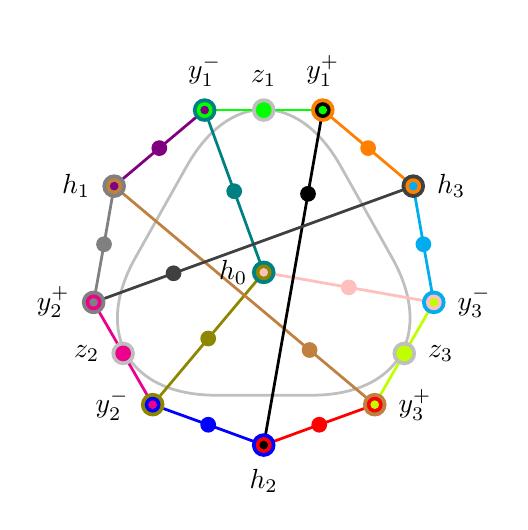
\begin{tikzpicture}  [scale=0.3]

\newdimen\ms
\ms=0.1cm

\tikzstyle{every path}=[line width=1pt]
\tikzstyle{c3}=[circle,inner sep={\ms/8},minimum size=3*\ms]
\tikzstyle{c2}=[circle,inner sep={\ms/8},minimum size=2*\ms]
\tikzstyle{c1}=[circle,inner sep={\ms/8},minimum size=1.1*\ms]



		% Define positions of all observables
		\path
     (-2.50, 6.87    ) coordinate(2)     % $y_1^-
			  (-6.33,   3.65  ) coordinate(4)    % h_1
			  (-7.20, -1.27   ) coordinate(6)       % y_2^+
			  (-4.70, -5.60   ) coordinate(8)       % y_2^-
			  (0, -7.31       ) coordinate(10)       % h_2
			  (4.70, -5.60    ) coordinate(12)        % y_3^+$
     (7.20, -1.27    ) coordinate(14)       % y_3^-
			  (6.33, 3.65     ) coordinate(16)       % h_3
			  (2.50, 6.87     ) coordinate(18)    % y_1^+

			  (0, 6.87        ) coordinate(1)     % z1
			  (-4.42, 5.26    ) coordinate(3)
			  (-6.76, 1.19    ) coordinate(5)
			  (-5.95, -3.43   ) coordinate(7)     % z2
			  (-2.35, -6.45   ) coordinate(9)
     (2.35, -6.45    ) coordinate(11)
			  (5.95,-3.43     ) coordinate(13)    % z3
			  (6.76, 1.19     ) coordinate(15)
		   (4.42, 5.26     ) coordinate(17)

     (0,0) coordinate(19)


(0, 10.3       ) coordinate(20)     % ze1
			  (-8.7, -5.2    ) coordinate(21)     % ze2
			  (8.7,-5.2    ) coordinate(22)    % ze3


     (-1.25, 3.435 ) coordinate(23)
     (3.60, -0.635 ) coordinate(24)
     (-2.35, -2.80 ) coordinate(25)
% h1={-6.33,   3.65  }; h3p={4.70, -5.60    } ; h1d2=  (h1+h3p )/2 ; c1=  (h1d2+h3p )/2
     (1.9425, -3.2875) coordinate(26)
% h2={0, -7.31    }; h1p={2.50, 6.87   } ; h2d2=  (h2+h1p )/2 ; c2=  (h2d2+h1p )/2
     (1.875, 3.325) coordinate(27)
% h3={6.33, 3.65    }; h2p={-7.20, -1.27    } ; h3d2=  (h3+h2p )/2 ; c3=  (h3d2+h2p )/2
     (-3.8175, -0.04) coordinate(28)
;

%(4.70-6.33,   3.65  -5.60   ) coordinate(4)    % h_1

	
		% Draw all the context curves
		
\draw [rounded corners=20mm,color=lightgray]     (20) -- (21) -- (22) --  cycle;


\draw [color=green] (18) -- (1) -- (2);
\draw [color=violet] (2) -- (3) -- (4);
\draw [color=gray] (4) -- (5) -- (6);
\draw [color=magenta] (6) -- (7) -- (8);
\draw [color=blue] (8) -- (9) -- (10);
\draw [color=red] (10) -- (11) -- (12) ;

\draw [color=lime] (12) -- (13) -- (14);
\draw [color=cyan] (14) -- (15) -- (16);
\draw [color=orange] (16) -- (17) -- (18);

\draw [color=teal] (19) -- (2);
\draw [color=olive] (19) -- (8);
\draw [color=pink] (19) -- (14);

\draw [color=brown] (4) -- (12);
\draw [color=black] (10) -- (18);
\draw [color=darkgray] (16) -- (6);





%\draw [color=lightgray](0,0) circle (6.87);



\draw (19) coordinate[c3,fill=teal];
\draw (19) coordinate[c2,fill=olive];
\draw (19) coordinate[c1,fill=pink,label=180:$h_0$];


\draw (1)  coordinate[c3,fill=lightgray,label=90:$z_1$];
\draw (1)  coordinate[c2,fill=green];

\draw (2)  coordinate[c3,fill=teal,label=90:$y_1^-$];
\draw (2)  coordinate[c2,fill=green];
\draw (2)  coordinate[c1,fill=violet];

\draw (3)  coordinate[c2,fill=violet];

\draw (4)  coordinate[c3,fill=gray,label=180:$h_1$];
\draw (4)  coordinate[c2,fill=brown];
\draw (4)  coordinate[c1,fill=violet];

\draw (5)  coordinate[c2,fill=gray,label=0:$ $];

\draw (6)  coordinate[c3,fill=darkgray,fill=gray,label=180:$y_2^+$];
\draw (6)  coordinate[c2,fill=magenta];
\draw (6)  coordinate[c1,fill=gray];

\draw (7)  coordinate[c3,fill=lightgray,label=180:$z_2$];
\draw (7)  coordinate[c2,fill=magenta];

\draw (8)  coordinate[c3,fill=olive,label=180:$y_2^-$];
\draw (8)  coordinate[c2,fill=blue];
\draw (8)  coordinate[c1,fill=magenta];

\draw (9)  coordinate[c2,fill=blue,label=0:$ $];

\draw (10) coordinate[c3,fill=blue,label=270:$h_2$];
\draw (10) coordinate[c2,fill=red];
\draw (10) coordinate[c1,fill=black];

\draw (11) coordinate[c2,fill=red,label=0:$ $];

\draw (12) coordinate[c3,fill=brown,label=0:$y_3^+$];
\draw (12) coordinate[c2,fill=red];
\draw (12) coordinate[c1,fill=lime];

\draw (13) coordinate[c3,fill=lightgray,label=0:$z_3$];
\draw (13) coordinate[c2,fill=lime];

\draw (14) coordinate[c3,fill=cyan,label=0:$y_3^-$];
\draw (14) coordinate[c2,fill=pink];
\draw (14) coordinate[c1,fill=lime];

\draw (15) coordinate[c2,fill=cyan,label=0:$ $];

\draw (16) coordinate[c3,fill=darkgray,label=0:$h_3$];
\draw (16) coordinate[c2,fill=orange];
\draw (16) coordinate[c1,fill=cyan];

\draw (17) coordinate[c2,fill=orange,label=0:$ $];

\draw (18) coordinate[c3,fill=orange,label=90:$y_1^+$];
\draw (18) coordinate[c2,fill=black];
\draw (18) coordinate[c1,fill=green];

\draw (23) coordinate[c2,fill=teal];
\draw (24) coordinate[c2,fill=pink];
\draw (25) coordinate[c2,fill=olive];
\draw (26) coordinate[c2,fill=brown];
\draw (27) coordinate[c2,fill=black];
\draw (28) coordinate[c2,fill=darkgray];


		\end{tikzpicture}
&
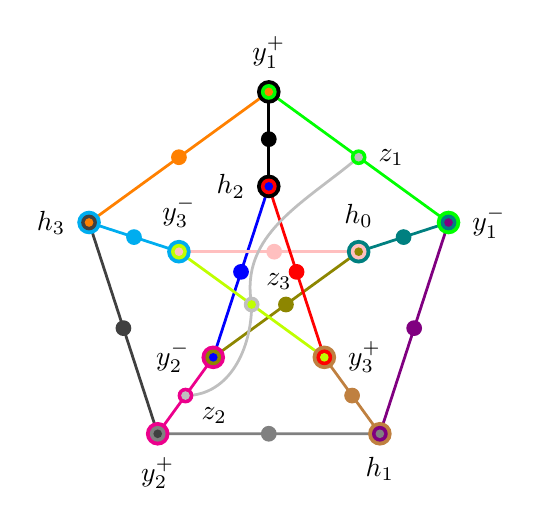
\begin{tikzpicture}  [scale=0.4]
\newdimen\ms
\ms=0.1cm

\tikzstyle{every path}=[line width=1pt]
\tikzstyle{c3}=[circle,inner sep={\ms/8},minimum size=3*\ms]
\tikzstyle{c2}=[circle,inner sep={\ms/8},minimum size=2*\ms]
\tikzstyle{c1}=[circle,inner sep={\ms/8},minimum size=1.1*\ms]

% Radius of regular polygons
\newdimen\R
\R=6cm
%\r= { \R * sqrt(3)/2}
\newdimen\K
\K=3cm

% Define positions of all observables
\path
  ({90 + 0 * 360 /5}:\R      ) coordinate(1)
  ({90 + 360 /10 + 0 * 360/5} : {\R * 0.6881/0.8507} ) coordinate(2)
  ({90 + 1 * 360 /5}:\R   ) coordinate(3)
  ({90 + 360 /10 + 1 * 360/5} : {\R * 0.6881/0.8507} ) coordinate(4)
  ({90 + 2 * 360 /5}:\R  ) coordinate(5)
  ({90 + 360 /10 + 2 * 360/5} : {\R * 0.6881/0.8507} ) coordinate(6)
  ({90 + 3 * 360 /5}:\R  ) coordinate(7)
  ({90 + 360 /10 + 3 * 360/5} : {\R * 0.6881/0.8507} ) coordinate(8)
  ({90 + 4 * 360 /5}:\R     ) coordinate(9)
  ({90 + 360 /10 + 4 * 360/5} : {\R * 0.6881/0.8507} ) coordinate(10)
  ({90 + 0 * 360 /5}:\K      ) coordinate(11)
  ({90 + 360 /10 + 0 * 360/5} : {\K * 0.6881/0.8507} ) coordinate(12)
  ({90 + 1 * 360 /5}:\K   ) coordinate(13)
  ({90 + 360 /10 + 1 * 360/5} : {\K * 0.6881/0.8507} ) coordinate(14)
  ({90 + 2 * 360 /5}:\K  ) coordinate(15)
  ({90 + 360 /10 + 2 * 360/5} : {\K * 0.6881/0.8507} ) coordinate(16)
  ({90 + 3 * 360 /5}:\K  ) coordinate(17)
  ({90 + 360 /10 + 3 * 360/5} : {\R * 0.6881/0.8507} ) coordinate(18)
  ({90 + 4 * 360 /5}:\K     ) coordinate(19)
  ({90 + 360 /10 + 4 * 360/5} : {\K * 0.6881/0.8507} ) coordinate(20)

  ({90 + 2 * 360 /5}:{(\R+\K)/2}) coordinate(21)

;

% draw contexts

\draw [color=orange] (1) -- (2) -- (3);
\draw [color=darkgray] (3) -- (4) -- (5);
\draw [color=gray] (5) -- (6) -- (7);
\draw [color=violet] (7) -- (8) -- (9);
\draw [color=green] (9) -- (10) -- (1);    %

\draw [color=blue] (11) -- (15) ;
\draw [color=olive] (15) -- (19);
\draw [color=pink] (19) -- (13);
\draw [color=lime] (13) -- (17);
\draw [color=red] (17) -- (11);

\draw ($ (11) !.5! (15) $) coordinate[c2,fill=blue];  %
\draw ($ (15) !.5! (19) $) coordinate[c2,fill=olive];  %
\draw ($ (19) !.47! (13) $) coordinate[c2,fill=pink];  %
\draw ($ (17) !.5! (11) $) coordinate[c2,fill=red];  %

\draw [color=black] (1) -- (11);
\draw [color=cyan] (3) -- (13);
\draw [color=magenta] (5) -- (15);
\draw [color=brown] (7) -- (17);
\draw [color=teal] (9) -- (19);

\draw ($ (1) !.5! (11) $) coordinate[c2,fill=black];  %
\draw ($ (3) !.5! (13) $) coordinate[c2,fill=cyan];  %
\draw ($ (7) !.5! (17) $) coordinate[c2,fill=brown];  %
\draw ($ (9) !.5! (19) $) coordinate[c2,fill=teal];  %

\draw [color=lightgray] (10)  to   [out=-140,in=100] ($ (13) !.5! (17) $)  to   [out=-90,in=0] (21);
%
%%
%% draw atoms
%%
%
\draw (1) coordinate[c3,fill=black,label=90:$y_1^+$];  %
\draw (1) coordinate[c2,fill=green];   %
\draw (1) coordinate[c1,fill=orange];  %
%
\draw (2) coordinate[c2,fill=orange];    %
%
\draw (3) coordinate[c3,fill=cyan,label=180:$h_3$];   %
\draw (3) coordinate[c2,fill=darkgray]; %
\draw (3) coordinate[c1,fill=orange];  %
%
\draw (4) coordinate[c2,fill=darkgray];  %
%
\draw (5) coordinate[c3,fill=magenta,label=270:$y_2^+$];  %
\draw (5) coordinate[c2,fill=gray];  %
\draw (5) coordinate[c1,fill=darkgray];  %
%
\draw (6) coordinate[c2,fill=gray];
%
\draw (7) coordinate[c3,fill=brown,label=270:$h_1$];  %
\draw (7) coordinate[c2,fill=violet];  %
\draw (7) coordinate[c1,fill=gray];  %
%
\draw (8) coordinate[c2,fill=violet];  %
%
\draw (9) coordinate[c3,fill=green,label=0:$y_1^-$];
\draw (9) coordinate[c2,fill=teal];
\draw (9) coordinate[c1,fill=violet];  %
%
\draw (10) coordinate[c2,fill=green,label=0:$z_1$];  %
\draw (10) coordinate[c1,fill=lightgray];  %
%
\draw (11) coordinate[c3,fill=black,label=180:$h_2$];  %
\draw (11) coordinate[c2,fill=red];  %
\draw (11) coordinate[c1,fill=blue]; %
%
%
\draw (13) coordinate[c3,fill=cyan,label=90:$y_3^-$]; %
\draw (13) coordinate[c2,fill=lime];  %
\draw (13) coordinate[c1,fill=pink];  %
%
\draw (15) coordinate[c3,fill=magenta,label=180:$y_2^-$]; %
\draw (15) coordinate[c2,fill=olive]; %
\draw (15) coordinate[c1,fill=blue]; %

\draw (17) coordinate[c3,fill=brown,label=0:$y_3^+$];  %
\draw (17) coordinate[c2,fill=red];   %
\draw (17) coordinate[c1,fill=lime]; %

\draw (19) coordinate[c3,fill=teal,label=90:$h_0$]; %
\draw (19) coordinate[c2,fill=pink]; %
\draw (19) coordinate[c1,fill=olive]; %

%
\draw (21) coordinate[c2,fill=magenta];  %
\draw (21) coordinate[c1,fill=lightgray,label=-15:$z_2$];  %

\draw ($ (13) !.5! (17) $) coordinate[c2,fill=lightgray];  %
\draw ($ (13) !.5! (17) $) coordinate[c1,fill=lime,label=45:$z_3$];  %


\end{tikzpicture}
\\
(a)&(b)
\end{tabular}
\end{center}
\caption{\label{2017-b-f-Yu-2012} (Color online) Two equivalent representations of a Petersen graph-like
(with one additional context connecting
$z_1$,
$z_2$, and
$z_3$)
Greechie diagram of the logic considered by Yu and Oh~\cite[Fig.~2]{Yu-2012}.
The set of two-valued states enforces at most one of the four atoms $h_0,h_1,h_2,h_3$ to be 1.
The logic has a (quantum) realization in $\mathbb{R}^3$
consisting of the 25 projections;  associated with the one dimensional subspaces
spanned by  the 13 vectors from the origin $\left(0,0,0\right)^\intercal$ to
$z_1 = \left( 1, 0, 0 \right)^\intercal $,
$z_2 = \left( 0, 1, 0 \right)^\intercal $,
$z_3 = \left( 0, 0, 1 \right)^\intercal $,
$y^-_1 = \left( 0, 1, -1 \right)^\intercal $,
$y^-_2 = \left( 1, 0, -1 \right)^\intercal $,
$y^-_3 = \left( 1, -1, 0 \right)^\intercal $,
$y^+_1 = \left( 0, 1, 1 \right)^\intercal $,
$y^+_2 = \left( 1, 0, 1 \right)^\intercal $,
$y^+_3 = \left( 1, 1, 0 \right)^\intercal $,
$h_0 = \left( 1, 1, 1 \right)^\intercal $,
$h_1 = \left( -1, 1, 1 \right)^\intercal $,
$h_2 = \left( 1, -1, 1 \right)^\intercal $,
$h_3 = \left( 1, 1, -1 \right)^\intercal $,
respectively~\cite{Yu-2012}.
}
\end{figure*}


\subsubsection{Kochen-Specker's $\Gamma_1$ ``true implies true'' logic}
\label{2017-b-s-tit}

A small extension of the Specker bug logic by two contexts extending from $a_1$ and $a_7$, both intertwining at a point $c$ renders a logic which facilitates that,
whenever $a_1$ is true, so must be an atom $b_1$, which is element in the context $\{a_7,c,b_1\}$,
as depicted in Fig.~\ref{2017-b-f-gamma1}.
\begin{figure}
\begin{center}
%%
%%
%%
%%
%%TexCad Options
%%\grade{\off}
%%\emlines{\off}
%%\beziermacro{\off}
%%\reduce{\on}
%%\snapping{\off}
%%\quality{0.20}
%%\graddiff{0.01}
%%\snapasp{1}
%%\zoom{1.00}
%\unitlength 0.45mm
%%%  \allinethickness{1pt} %\thicklines %\linethickness{1pt}
%%  \allinethickness{2pt}
%\begin{picture}(168.00,80.00)
%\put(25.00,7.33){\color{gray}\line(1,0){60.00}}
%\put(25.00,47.33){\color{red}\line(1,0){60.00}}
%\put(55.00,7.33){\color{cyan}\line(0,1){40.00}}
%\put(25.00,7.33){\color{blue}\line(-1,1){20.00}}
%\put(5.00,27.33){\color{green}\line(1,1){20.00}}
%\put(85.00,7.33){\color{magenta}\line(1,1){20.00}}
%\put(105.00,27.33){\color{orange}\line(-1,1){20.00}}
%\put(134.50,27.33){\color{violet}\line(0,-1){20.00}}
%%
%\put(105.00,27.33){\color{pink}\line(1,0){60.00}}
%\put(69, 27.33){\color{violet}\oval(130, 80)[t]}
%%{\color{violet}\qbezier(5,27.33)(32.5,140)(134.76,27.33)}
%%
%\put(134.50,0){\makebox(0,0)[rc]{$b_7$}}
%\put(24.67,55.00){\makebox(0,0)[rc]{$a_3$}}
%\put(55.33,55.00){\makebox(0,0)[cc]{$a_4$}}
%\put(85.33,55.00){\makebox(0,0)[lc]{$a_5$}}
%\put(27.00,37.33){\makebox(0,0)[rc]{$a_2$}}
%\put(99.33,40.00){\makebox(0,0)[lc]{$a_6$}}
%\put(0.00,27.33){\makebox(0,0)[rc]{$a_1$}}
%\put(113.00,32.33){\makebox(0,0)[lc]{$a_7$}}
%\put(60.33,31.33){\makebox(0,0)[lc]{$a_{13}$}}
%\put(9.00,13.33){\makebox(0,0)[rc]{$a_{12}$}}
%\put(99.67,13.33){\makebox(0,0)[lc]{$a_8$}}
%\put(24.67,0){\makebox(0,0)[rc]{$a_{11}$}}
%\put(55.33,0){\makebox(0,0)[cc]{$a_{10}$}}
%\put(85.33,0){\makebox(0,0)[lc]{$a_9$}}
%\put(134.50,7){\color{violet}\circle*{1.00}}
%\put(134.50,7){\color{violet}\circle*{2.00}}
%\put(15.00,17.09){\color{blue}\circle*{1.00}}
%\put(15.00,17.09){\color{blue}\circle*{2.00}}
%\put(25.00,7.33){\color{blue}\circle*{1.00}}
%\put(25.00,7.33){\color{blue}\circle*{2.00}}
%\put(25.00,7.33){\color{gray}\circle*{3.00}}
%\put(55.00,27.33){\color{cyan}\circle*{1.00}}
%\put(55.00,27.33){\color{cyan}\circle*{2.00}}
%\put(85.00,7.33){\color{gray}\circle*{1.00}}
%\put(85.00,7.33){\color{gray}\circle*{2.00}}
%\put(85.00,7.33){\color{magenta}\circle*{3.00}}
%\put(95.00,17.33){\color{magenta}\circle*{1.00}}
%\put(95.00,17.33){\color{magenta}\circle*{2.00}}
%\put(5.00,27.33){\color{green}\circle*{1.00}}
%\put(5.00,27.33){\color{green}\circle*{2.00}}
%\put(5.00,27.33){\color{green}\circle*{3.00}}
%\put(5.00,27.33){\color{blue}\circle*{3.0}}
%\put(5.00,27.33){\color{violet}\circle*{3.00}}
%\put(15.00,37.33){\color{green}\circle*{1.00}}
%\put(15.00,37.33){\color{green}\circle*{2.00}}
%\put(25.00,47.33){\color{green}\circle*{1.00}}
%\put(25.00,47.33){\color{green}\circle*{2.00}}
%\put(25.00,47.33){\color{red}\circle*{3.00}}
%\put(55.00,47.33){\color{red}\circle*{1.00}}
%\put(55.00,47.33){\color{red}\circle*{2.00}}
%\put(55.00,47.33){\color{cyan}\circle*{3.00}}
%\put(85.00,47.33){\color{red}\circle*{1.00}}
%\put(85.00,47.33){\color{red}\circle*{2.00}}
%\put(85.00,47.33){\color{orange}\circle*{3.00}}
%\put(55.00,7.33){\color{gray}\circle*{1.00}}
%\put(55.00,7.33){\color{gray}\circle*{2.00}}
%\put(55.00,7.33){\color{cyan}\circle*{3.00}}
%\put(105,27.33){\color{orange}\circle*{1.00}}
%\put(105,27.33){\color{orange}\circle*{2.00}}
%\put(105,27.33){\color{magenta}\circle*{3.00}}
%\put(105,27.33){\color{pink}\circle*{3.00}}
%\put(95.00,37.33){\color{orange}\circle*{1.00}}
%\put(95.00,37.33){\color{orange}\circle*{2.00}}
%
%\put(165,27.33){\color{pink}\circle*{1.00}}
%\put(165,27.33){\color{pink}\circle*{2.00}}
%\put(135,27.33){\color{pink}\circle*{1.00}}
%\put(134.76,27.33){\color{pink}\circle*{2.00}}
%\put(134.76,27.33){\color{violet}\circle*{3.00}}
%\put(140.00,32.33){\makebox(0,0)[lc]{$c$}}
%\put(168.00,27.33){\makebox(0,0)[lc]{$b_1$}}
%\end{picture}
%
%
% This is a LaTeX picture output by TeXCAD.
% File name: [1.pic].
% Version of TeXCAD: 4.3
% Reference / build: 30-Jun-2012 (rev. 105)
% For new versions, check: http://texcad.sf.net/
% Options on the following lines.
%\grade{\off}
%\emlines{\off}
%\epic{\off}
%\beziermacro{\on}
%\reduce{\on}
%\snapping{\off}
%\quality{0.200}
%\graddiff{0.010}
%\snapasp{1}
%\zoom{8.0000}
%\unitlength 1mm % = 2.845pt
%\linethickness{0.4pt}
\unitlength 0.55mm
%  \allinethickness{2pt}
\ifx\plotpoint\undefined\newsavebox{\plotpoint}\fi % GNUPLOT compatibility
\begin{picture}(152,120)(0,0)
%
\put(15.455,85.051){\color{gray}\line(0,-1){60}}
%\put(144.545,85.051){\color{gray}\line(0,-1){60}}
\put(55.455,85.051){\color{red}\line(0,-1){60}}
%\put(104.545,85.051){\color{red}\line(0,-1){60}}
\put(15.455,55.051){\color{cyan}\line(1,0){40}}
%\put(144.545,55.051){\color{cyan}\line(-1,0){40}}
\put(15.455,85.051){\color{blue}\line(1,1){20}}
%\put(144.545,85.051){\color{blue}\line(-1,1){20}}
\put(35.455,105.051){\color{green}\line(1,-1){20}}
%\put(124.545,105.051){\color{green}\line(-1,-1){20}}
\put(15.455,25.051){\color{magenta}\line(1,-1){20}}
%\put(144.545,25.051){\color{magenta}\line(-1,-1){20}}
\put(35.455,5.051){\color{orange}\line(1,1){20}}
%\put(124.545,5.051){\color{orange}\line(-1,1){20}}
%
%
\color{pink}\qbezier(35.5,5.25)(68,5.625)(80,55)
\color{violet}\qbezier(124.5,5.25)(92,5.625)(80,55)
\color{violet}\qbezier(35.5,104.5)(68,104.125)(80,54.75)
\color{pink}\qbezier(124.5,104.5)(92,104.125)(80,54.75)
{\color{black}
%
\put(62.125,80.381){\makebox(0,0)[b]{$a_3$}}
%\put(98.875,80.381){\makebox(0,0)[b]{$b_3$}}
\put(62.125,54.721){\makebox(0,0)[]{$a_4$}}
%\put(98.875,54.721){\makebox(0,0)[]{$b_4$}}
\put(62.125,26.721){\makebox(0,0)[t]{$a_5$}}
%\put(98.875,26.721){\makebox(0,0)[t]{$b_5$}}
\put(43.125,85.051){\makebox(0,0)[b]{$a_2$}}
%\put(116.875,85.051){\makebox(0,0)[b]{$b_2$}}
\put(43.125,22.721){\makebox(0,0)[t]{$a_6$}}
%\put(116.875,22.721){\makebox(0,0)[t]{$b_6$}}
\put(34.455,110.051){\makebox(0,0)[b]{$a_1$}}
 \put(125.545,110.051){\makebox(0,0)[b]{$b_1$}}
\put(34.455,0){\makebox(0,0)[t]{$a_7$}}
 \put(125.545,0){\makebox(0,0)[t]{$b_7$}}
\put(35,49.721){\makebox(0,0)[t]{$a_{13}$}}
%\put(125,49.721){\makebox(0,0)[t]{$b_{13}$}}
\put(21.455,101.051){\makebox(0,0)[b]{$a_{12}$}}
%\put(138.545,101.051){\makebox(0,0)[b]{$b_{12}$}}
\put(21.455,10.381){\makebox(0,0)[t]{$a_8$}}
%\put(138.545,10.381){\makebox(0,0)[t]{$b_8$}}
\put(8.075,85.381){\makebox(0,0)[b]{$a_{11}$}}
%\put(151.925,85.381){\makebox(0,0)[b]{$b_{11}$}}
\put(8.075,54.721){\makebox(0,0)[]{$a_{10}$}}
%\put(151.925,54.721){\makebox(0,0)[]{$b_{10}$}}
\put(8.075,24.721){\makebox(0,0)[t]{$a_9$}}
%\put(151.925,24.721){\makebox(0,0)[t]{$b_9$}}
\put(85,55){\makebox(0,0)[t]{$c$}}
\put(25.215,95.051){\color{blue}\circle*{3}}
%
%
%
\put(15.455,85.051){\color{gray}\circle*{6}}
\put(15.455,85.051){\color{blue}\circle*{3}}
%
%
%
 \put(35.455,55.051){\color{cyan}\circle*{3}}
%
%
\put(15.455,25.051){\color{magenta}\circle*{6}}
\put(15.455,25.051){\color{gray}\circle*{3}}
%
%
%
\put(25.455,15.051){\color{magenta}\circle*{3}}
%
%
%
\put(35.455,105.051){\color{violet}\circle*{8}}
\put(35.455,105.051){\color{blue}\circle*{6}}
\put(35.455,105.051){\color{green}\circle*{3}}
%
%
%
%
\put(45.455,95.051){\color{green}\circle*{3}}
%
%
\put(55.455,85.051){\color{red}\circle*{6}}
\put(55.455,85.051){\color{green}\circle*{3}}
%
%
%
\put(55.455,55.051){\color{cyan}\circle*{6}}
\put(55.455,55.051){\color{red}\circle*{3}}
%
%
\put(55.455,25.051){\color{orange}\circle*{6}}
\put(55.455,25.051){\color{red}\circle*{3}}
%
%
%
\put(15.455,55.051){\color{gray}\circle*{6}}
\put(15.455,55.051){\color{cyan}\circle*{3}}
%
%
%
\put(35.455,5.291){\color{pink}\circle*{8}}
\put(35.455,5.291){\color{magenta}\circle*{6}}
\put(35.455,5.291){\color{orange}\circle*{3}}
%
%
%
%
%
\put(45.455,15.051){\color{orange}\circle*{3}}
%
\put(80,55){\color{violet}\circle*{6}}
\put(80,55){\color{pink}\circle*{3}}
\put(124.545,5.291){\color{violet}\circle*{3}}
\put(124.545,105){\color{pink}\circle*{3}}
}
\end{picture}
\end{center}
\caption{\label{2017-b-f-gamma1} (Color online) Greechie diagram of the Kochen-Specker $\Gamma_1$ logic~\cite[p.~68]{kochen1},
which is an extension of the Specker bug logic by two intertwining contexts at the bug's extremities.
The logic has a (quantum) realization in $\mathbb{R}^3$
consisting of the 16 projections associated with the one dimensional subspaces
spanned by  the vectors from the origin $\left(0,0,0\right)^\intercal$ to
the 13 points mentioned in Fig.~\ref{2001-cesena-f2}, as well as
%$a_{1}     = \left(    1,\sqrt{2},0     \right)^\intercal $,
%$a_{2}     = \left(\sqrt{2}, -1, -3 \right)^\intercal $,
%$a_{3}     = \left(   \sqrt{2},-1,1     \right)^\intercal $,
%$a_{4}     = \left(    0,1,1     \right)^\intercal $,
%$a_{5}     = \left(   \sqrt{2},1,-1     \right)^\intercal $,
%$a_{6}     = \left(\sqrt{2}, 1, 3 \right)^\intercal $,
%$a_{7}     = \left(    -1,\sqrt{2},0     \right)^\intercal $,
%$a_{8}     = \left(\sqrt{2}, 1, -3 \right)^\intercal $,
%$a_{9}     = \left(   \sqrt{2},1,1     \right)^\intercal $,
%$a_{10}     = \left(    0,1,-1     \right)^\intercal $,
%$a_{11}     = \left(   \sqrt{2},-1,-1     \right)^\intercal $,
%$a_{12}     = \left(\sqrt{2}, -1, 3 \right)^\intercal $,
%$a_{13}     = \left(    1,0,0     \right)^\intercal $,
 $c          = \left(    0,0,1     \right)^\intercal $,
 $b_{1}     = \left(   \sqrt{2},1,0     \right)^\intercal $,
%$b_{2}     = \left(1, -\sqrt{2}, -3 \right)^\intercal $,
%$b_{3}     = \left(    -1,\sqrt{2},-1     \right)^\intercal $,
%$b_{4}     = \left(    1,0,-1     \right)^\intercal $,
%$b_{5}     = \left(    1,\sqrt{2},1     \right)^\intercal $,
%$b_{6}     = \left(1, \sqrt{2}, -3 \right)^\intercal $,
 $b_{7}     = \left(   \sqrt{2},-1,0     \right)^\intercal $,
%$b_{8}     = \left(1, \sqrt{2}, 3 \right)^\intercal $,
%$b_{9}     = \left(    1,\sqrt{2},-1     \right)^\intercal $,
%$b_{10}     = \left(    1,0,1     \right)^\intercal $,
%$b_{11}     = \left(    -1,\sqrt{2},1     \right)^\intercal $,
%$b_{12}     = \left(-1, \sqrt{2}, -3 \right)^\intercal $,
%$b_{13}     = \left(    0,1,0     \right)^\intercal $,
respectively~\cite[p.~206, Fig.~1]{tkadlec-96}.
}
\end{figure}

The reduction of some probabilities of atoms at intertwined contexts yields ($q_1, q_7$ are the probabilities on $b_1, b_7$, respectively),
additionally to Eq.~(\ref{2015-s-e2}),
\begin{equation}
\begin{split}
p_1 - p_7 = q_1 - q_7
,
\end{split}
\label{2017-b-spa2l}
\end{equation}
which, as  can  be derived also explicitly by taking into account admissibility,
implies that, for all the 112 two-valued states, if $p_1=1$, then [from Eq.~(\ref{2015-s-e2})] $p_7=0$,
and $q_1=1$ as well as $q_7 = 1 - q_1 = 0$.

Besides the  quantum mechanical realization of this logic in terms of propositions identified with projection operators
corresponding to vectors in three-dimensional Hilbert space
Tkadlec and this author~\cite[p.~5387, Fig.~4]{svozil-tkadlec}
(see also Tkadlec~\cite[p.~206, Fig.~1]{tkadlec-96}) have given  an explicit collection of such vectors.
As Tkadlec has observed (cf. Ref.~\cite[p.~5390]{svozil-tkadlec}, and Ref.~\cite[p.]{tkadlec-01}),
the original realization suggested by Kochen and Specker~\cite{kochen1} appears to be a little bit ``buggy''
as they did not use the right angle between $a_1$ and $a_7$, but this could be rectified.

Other ``true implies true'' logics have been introduced by Belinfante~\cite[Fig.~C.l. p.~67]{Belinfante-73},
Pitowsky~\cite[p.~394]{Pitowsky-1982-subs},
Clifton~\cite{clifton-93,Johansen-1994,Vermaas-1994},
as well as Cabello and G. Garc{\'{i}}a-Alcaine~\cite[Lemma~1]{Cabello-1996-bks-fd}.


Notice that, if a second Specker bug logic is placed along $b_1$ and $b_7$,
just as in the Kochen-Specker $\Gamma_3$ logic~\cite[p.~70]{kochen1},
this imposes an additional ``true implies false'' condition; together with the
 ``true implies false'' condition of the first logic this
implies the fact that $a_1$ and $a_7$ can no longer be separated by some two-valued state: whenever one is true,
the other one must be true as well, and {\em vice versa}.
This Kochen-Specker logic $\Gamma_3$ will be discussed in the next Section~\ref{2017-b-bugscombino}.

Notice further that if we manage to iterate this process in such a manner that,
with every $i$th iteration we place another Kochen-Specker $\Gamma_3$ logic  along $b_i$,
while at the same time increasing the angle between $b_i$ and $b_1$,
then eventually we shall arrive at a situation in which $b_1$ and $b_i$ are part of a context
(in terms of Hilbert space: they correspond to orthogonal vectors).
But admissibility disallows two-valued measures with more than one, and in particular,
two ``true'' atoms within a single block. As a consequence, if such a configuration is
realizable (say, in 3-dimensional Hilbert space), then it cannot have any two-valued state
satisfying the admissibility criteria.
This is the Kochen-Specker theorem, as exposed in the  Kochen-Specker $\Gamma_3$ logic~\cite[p.~69]{kochen1},
which will be discussed in Section~\ref{2017-b-c-lwtvs}.


\subsubsection{Combo of two linked Specker bug logics inducing non-separability}
\label{2017-b-bugscombino}

As we are heading toward  logics with less and less ``rich'' set of two-valued states we are approaching
a logic   depicted in Fig.~\ref{2017-b-f-twobugs}
which is a combination of two Specker bug logics linked by two external contexts.
It is the $\Gamma_3$-configuration of Kochen-Specker~\cite[p.~70]{kochen1}
with a set of two-valued states which is no longer separating:
In this case one obtains the ``one-one'' and ``zero-zero rules''~\cite{svozil-2006-omni},
stating that  $a_1$ occurs if and only if $b_1$ occurs
(likewise, $a_7$ occurs if and only if $b_7$ occurs):
Suppose $v$ is a two-valued state on the $\Gamma_3$-configuration of Kochen-Specker.
Whenever $v(a_1)=1$, then $v(c)=0$ because it is in the same context $\{a_1,c,b_7\}$ as $a_1$.
Furthermore, because of Eq.~(\ref{2015-s-e2}), whenever $v(a_1)=1$, then $v(a_7)=0$.
Because $b_1$ is in the same context $\{a_7,c,b_1\}$ as $a_7$ and $c$, because of admissibility, $v(b_1)=1$.
Conversely, by symmetry, whenever $v(b_1)=1$, so must be $v(a_1)=1$.
Therefore it can never happen that either one of the two atoms $a_1$ and $b_1$ have different dichotomic values.
(Eq.~\ref{2017-b-spa2l} is compatible with these value assignments.)
The same is true for the pair of atoms  $a_7$ and $b_7$.

Note that one needs two Specker bug logics tied together (at their ``true implies false'' extremities)
to obtain non-separability;
just extending one to the
Kochen-Specker $\Gamma_1$ logic~\cite[p.~68]{kochen1} of Fig.~\ref{2017-b-f-gamma1}
discussed earlier to obtain ``true implies true'' would be insufficient.
Because in this case a consistent two-valued state exists for which $v(b_1)=v(b_7)=1$ and $v(a_1)=v(a_7)=0$,
thereby separating $a_1$ from $b_1$, and {\it vice versa}.
A second Specker bug logic is neded to elimitate this case; in particular, $v(b_1)=v(b_7)=1$.


\begin{figure}
\begin{center}
\begin{tabular}{c}
% This is a LaTeX picture output by TeXCAD.
% File name: [1.pic].
% Version of TeXCAD: 4.3
% Reference / build: 30-Jun-2012 (rev. 105)
% For new versions, check: http://texcad.sf.net/
% Options on the following lines.
%\grade{\off}
%\emlines{\off}
%\epic{\off}
%\beziermacro{\on}
%\reduce{\on}
%\snapping{\off}
%\quality{0.200}
%\graddiff{0.010}
%\snapasp{1}
%\zoom{8.0000}
%\unitlength 1mm % = 2.845pt
%\linethickness{0.4pt}
\unitlength 0.55mm
%  \allinethickness{2pt}
\ifx\plotpoint\undefined\newsavebox{\plotpoint}\fi % GNUPLOT compatibility
\begin{picture}(152,120)(0,0)
%
\put(15.455,85.051){\color{gray}\line(0,-1){60}}
\put(144.545,85.051){\color{gray}\line(0,-1){60}}
\put(55.455,85.051){\color{red}\line(0,-1){60}}
\put(104.545,85.051){\color{red}\line(0,-1){60}}
\put(15.455,55.051){\color{cyan}\line(1,0){40}}
\put(144.545,55.051){\color{cyan}\line(-1,0){40}}
\put(15.455,85.051){\color{blue}\line(1,1){20}}
\put(144.545,85.051){\color{blue}\line(-1,1){20}}
\put(35.455,105.051){\color{green}\line(1,-1){20}}
\put(124.545,105.051){\color{green}\line(-1,-1){20}}
\put(15.455,25.051){\color{magenta}\line(1,-1){20}}
\put(144.545,25.051){\color{magenta}\line(-1,-1){20}}
\put(35.455,5.051){\color{orange}\line(1,1){20}}
\put(124.545,5.051){\color{orange}\line(-1,1){20}}
%
%
\color{pink}\qbezier(35.5,5.25)(68,5.625)(80,55)
\color{violet}\qbezier(124.5,5.25)(92,5.625)(80,55)
\color{violet}\qbezier(35.5,104.5)(68,104.125)(80,54.75)
\color{pink}\qbezier(124.5,104.5)(92,104.125)(80,54.75)
{\color{black}
%
\put(62.125,80.381){\makebox(0,0)[b]{$a_3$}}
\put(98.875,80.381){\makebox(0,0)[b]{$b_3$}}
\put(62.125,54.721){\makebox(0,0)[]{$a_4$}}
\put(98.875,54.721){\makebox(0,0)[]{$b_4$}}
\put(62.125,26.721){\makebox(0,0)[t]{$a_5$}}
\put(98.875,26.721){\makebox(0,0)[t]{$b_5$}}
\put(43.125,85.051){\makebox(0,0)[b]{$a_2$}}
\put(116.875,85.051){\makebox(0,0)[b]{$b_2$}}
\put(43.125,22.721){\makebox(0,0)[t]{$a_6$}}
\put(116.875,22.721){\makebox(0,0)[t]{$b_6$}}
\put(34.455,110.051){\makebox(0,0)[b]{$a_1$}}
\put(125.545,110.051){\makebox(0,0)[b]{$b_1$}}
\put(34.455,0){\makebox(0,0)[t]{$a_7$}}
\put(125.545,0){\makebox(0,0)[t]{$b_7$}}
\put(35,49.721){\makebox(0,0)[t]{$a_{13}$}}
\put(125,49.721){\makebox(0,0)[t]{$b_{13}$}}
\put(21.455,101.051){\makebox(0,0)[b]{$a_{12}$}}
\put(138.545,101.051){\makebox(0,0)[b]{$b_{12}$}}
\put(21.455,10.381){\makebox(0,0)[t]{$a_8$}}
\put(138.545,10.381){\makebox(0,0)[t]{$b_8$}}
\put(8.075,85.381){\makebox(0,0)[b]{$a_{11}$}}
\put(151.925,85.381){\makebox(0,0)[b]{$b_{11}$}}
\put(8.075,54.721){\makebox(0,0)[]{$a_{10}$}}
\put(151.925,54.721){\makebox(0,0)[]{$b_{10}$}}
\put(8.075,24.721){\makebox(0,0)[t]{$a_9$}}
\put(151.925,24.721){\makebox(0,0)[t]{$b_9$}}
\put(85,55){\makebox(0,0)[t]{$c$}}
\put(25.215,95.051){\color{blue}\circle*{3}}
%
%
%
\put(15.455,85.051){\color{gray}\circle*{6}}
\put(15.455,85.051){\color{blue}\circle*{3}}
%
%
%
 \put(35.455,55.051){\color{cyan}\circle*{3}}
%
%
\put(15.455,25.051){\color{magenta}\circle*{6}}
\put(15.455,25.051){\color{gray}\circle*{3}}
%
%
%
\put(25.455,15.051){\color{magenta}\circle*{3}}
%
%
%
\put(35.455,105.051){\color{violet}\circle*{8}}
\put(35.455,105.051){\color{blue}\circle*{6}}
\put(35.455,105.051){\color{green}\circle*{3}}
%
%
%
%
\put(45.455,95.051){\color{green}\circle*{3}}
%
%
\put(55.455,85.051){\color{red}\circle*{6}}
\put(55.455,85.051){\color{green}\circle*{3}}
%
%
%
\put(55.455,55.051){\color{cyan}\circle*{6}}
\put(55.455,55.051){\color{red}\circle*{3}}
%
%
\put(55.455,25.051){\color{orange}\circle*{6}}
\put(55.455,25.051){\color{red}\circle*{3}}
%
%
%
\put(15.455,55.051){\color{gray}\circle*{6}}
\put(15.455,55.051){\color{cyan}\circle*{3}}
%
%
%
\put(35.455,5.291){\color{pink}\circle*{8}}
\put(35.455,5.291){\color{magenta}\circle*{6}}
\put(35.455,5.291){\color{orange}\circle*{3}}
%
\put(45.455,15.051){\color{orange}\circle*{3}}
%
\put(80,55){\color{violet}\circle*{6}}
\put(80,55){\color{pink}\circle*{3}}
\put(124.545,5.291){\color{violet}\circle*{8}}
\put(124.545,105){\color{pink}\circle*{8}}
%
%
%
%
\put(134.785,95.051){\color{blue}\circle*{3}}
\put(144.545,85.051){\color{gray}\circle*{6}}
\put(144.545,85.051){\color{blue}\circle*{3}}
\put(124.545,55.051){\color{cyan}\circle*{3}}
\put(144.545,25.051){\color{magenta}\circle*{6}}
\put(144.545,25.051){\color{gray}\circle*{3}}
\put(124.545,105){\color{green}\circle*{6}}
\put(124.545,105){\color{blue}\circle*{3}}
\put(134.545,15.051){\color{magenta}\circle*{3}}
\put(114.545,95.051){\color{green}\circle*{3}}
\put(104.545,85.051){\color{red}\circle*{6}}
\put(104.545,85.051){\color{green}\circle*{3}}
\put(104.545,55.051){\color{red}\circle*{6}}
\put(104.545,55.051){\color{cyan}\circle*{3}}
\put(104.545,25.051){\color{orange}\circle*{6}}
\put(104.545,25.051){\color{red}\circle*{3}}
\put(144.545,55.051){\color{gray}\circle*{6}}
\put(144.545,55.051){\color{cyan}\circle*{3}}
\put(124.545,5.291){\color{magenta}\circle*{6}}
\put(124.545,5.291){\color{orange}\circle*{3}}
\put(114.545,15.051){\color{orange}\circle*{3}}
}
\end{picture}
\end{tabular}
\end{center}
\caption{\label{2017-b-f-twobugs} (Color online) Greechie diagram of two linked Specker bug (cat's cradle) logics $\Gamma_3$.
The logic has a (quantum) realization in $\mathbb{R}^3$
consisting of the 27 projections associated with the one dimensional subspaces
spanned by  the vectors from the origin $\left(0,0,0\right)^\intercal$ to
the 13 points mentioned in Fig.~\ref{2001-cesena-f2},
the 3 points mentioned in Fig.~\ref{2017-b-f-gamma1}, as well as
%$a_{1}     = \left(    1,\sqrt{2},0     \right)^\intercal $,
%$a_{2}     = \left(\sqrt{2}, -1, -3 \right)^\intercal $,
%$a_{3}     = \left(   \sqrt{2},-1,1     \right)^\intercal $,
%$a_{4}     = \left(    0,1,1     \right)^\intercal $,
%$a_{5}     = \left(   \sqrt{2},1,-1     \right)^\intercal $,
%$a_{6}     = \left(\sqrt{2}, 1, 3 \right)^\intercal $,
%$a_{7}     = \left(    -1,\sqrt{2},0     \right)^\intercal $,
%$a_{8}     = \left(\sqrt{2}, 1, -3 \right)^\intercal $,
%$a_{9}     = \left(   \sqrt{2},1,1     \right)^\intercal $,
%$a_{10}     = \left(    0,1,-1     \right)^\intercal $,
%$a_{11}     = \left(   \sqrt{2},-1,-1     \right)^\intercal $,
%$a_{12}     = \left(\sqrt{2}, -1, 3 \right)^\intercal $,
%$a_{13}     = \left(    1,0,0     \right)^\intercal $,
% $c          = \left(    0,0,1     \right)^\intercal $,
% $b_{1}     = \left(   \sqrt{2},1,0     \right)^\intercal $,
$b_{2}     = \left(1, -\sqrt{2}, -3 \right)^\intercal $,
$b_{3}     = \left(    -1,\sqrt{2},-1     \right)^\intercal $,
$b_{4}     = \left(    1,0,-1     \right)^\intercal $,
$b_{5}     = \left(    1,\sqrt{2},1     \right)^\intercal $,
$b_{6}     = \left(1, \sqrt{2}, -3 \right)^\intercal $,
%$b_{7}     = \left(   \sqrt{2},-1,0     \right)^\intercal $,
$b_{8}     = \left(1, \sqrt{2}, 3 \right)^\intercal $,
$b_{9}     = \left(    1,\sqrt{2},-1     \right)^\intercal $,
$b_{10}     = \left(    1,0,1     \right)^\intercal $,
$b_{11}     = \left(    -1,\sqrt{2},1     \right)^\intercal $,
$b_{12}     = \left(-1, \sqrt{2}, -3 \right)^\intercal $,
$b_{13}     = \left(    0,1,0     \right)^\intercal $,
respectively~\cite[p.~206, Fig.~1]{tkadlec-96}.
Note that, with this realization, there is an additional context $\{ a_{13},c,b_{13}\}$ not drawn here,
which imposes an additional constraint $v(a_{13})+v(c)+v(b_{13})=1$ on any two-valued measure $v$.
(See also the proof of Proposition~7.2 in Ref.~\cite[p.~5392]{svozil-tkadlec}.)
}
\end{figure}

Besides the  quantum mechanical realization of this logic in terms of propositions which are projection operators
corresponding to vectors in three-dimensional Hilbert space suggested by Kochen and Specker~\cite{kochen1},
Tkadlec has given~\cite[p.~206, Fig.~1]{tkadlec-96}  an explicit collection of such vectors
(see also the proof of Proposition~7.2 in Ref.~\cite[p.~5392]{svozil-tkadlec}).


\subsubsection*{Probabilistic criteria against value definiteness from contraints on two-valued measures}
\label{2017-b-ss-pc}

The ``1-1'' or  ``true implies true'' rule can be taken as an operational criterion for quantization:
Suppose that one prepares a system to be in a pure state
corresponding to $a_1$, such that the preparation ensures that $v(a_1)=1$.
If the system is then measured along $b_1$, and the proposition that
the system is in state $b_1$  is found  to be {\em not} true, meaning that $v(b_1)\neq 1$ (the respective detector does not click),
then  one has established that the system is not performing classically,
because classically the set of two-valued states requires non-separability; that is, $v(a_1)=v(b_1)=1$.
With the Tkadlec directions taken from Figs.~\ref{2001-cesena-f2} and~\ref{2017-b-f-gamma1},
$\vert {\bf a}_1\rangle = (1/\sqrt{3}) \left(    1,\sqrt{2},0     \right)^\intercal$ and
$\vert {\bf b}_1\rangle = (1/\sqrt{3})\left(     \sqrt{2},1,0      \right)^\intercal$
so that the probability to find a quantized system prepared along $\vert {\bf a}_1\rangle$
and measured along $\vert {\bf b}_1\rangle$ is
$p_{a_1}(b_1) = \vert \langle {\bf b}_1 \vert {\bf a}_1 \rangle \vert^2=  8/9  $,
and that a violation of classicality should occur with probability $1/9$.
Of course, any other classical prediction, such as the ``1-0'' or ``true implies false'' rule,
or more general  classical predictions such as of Eq.~(\ref{2015-s-e2})
can also be taken as empirical criteria for non-classicality~\cite[Sect.~11.3.2.]{svozil-2016-s}).

Indeed, already Stairs~\cite[p.~588-589]{stairs83} has argued along similar lines for the Specker bug
``true implies false'' logic (a translation into our nomenclature
is:
$m1(1) \equiv a_1$,
$m2(1) \equiv a_3$,
$m2(2) \equiv a_5$,
$m2(3) \equiv a_4$,
$m3(1) \equiv a_{11}$,
$m3(2) \equiv a_9$,
$m3(3) \equiv a_{10}$,
$m4(1) \equiv a_7$).
Independently Clifton (there is a note added in proof to Stairs~\cite[p.~588-589]{stairs83})
presents asimilar argument, based upon (i) another ``true implies true'' logic~\cite[Sects.~II,III, Fig.~1]{clifton-93,Johansen-1994,Vermaas-1994}
inspired by Bell~\cite[Fig.~C.l. p.~67]{Belinfante-73} (cf. also Pitowsky~\cite[p.~394]{Pitowsky-1982-subs}),
as well as (ii) on the Specker bug logic~\cite[Sects.~IV, Fig.~2]{clifton-93}.
More recently Hardy~\cite{Hardy-92,Hardy-93,hardy-97}
as well as Cabello and
Garc{\'{i}}a-Alcaine and
others~\cite{Cabello-1995-ppks,cabello-96,cabello-97-nhvp,Badziag-2011,Cabello-2013-HP,Cabello-2013-Hardylike} discussed such scenarios.
These criteria for non-classicality are benchmarks aside from the Boole-Bell type polytope method,
and also different from the full Kochen-Specker theorem.



\subsubsection*{Imbedability}

As every algebra imbeddable in a Boolean algebra must have a separating set of two valued states,
this logic is no longer ``classical''
in the sense of ``homomorphically (structure-preserving) imbeddable.''
Nevertheless, two-valued states can still exist. It is just that these states can no longer differentiate
between the pairs of atoms $(a_1,b_1)$ as well as $(a_7,b_7)$.
Partition logics and their generalized urn or finite automata models fail to reproduce
two linked Specker bug logics resulting in a Kochen-Specker $\Gamma_3$ logic even at this stage.
Of course, the situation will become more dramatic with the non-existence of any kind of two-valued state
(interpretable as truth assignment) on certain logics associate with quantum propositions.

Complementarity and non-distributivity is not enough to characterize logics which do not have a quasi-classical
(partition logical, set theoretical) interpretation.
While in a certain, graph coloring sense the ``richness/scarcity'' and the {\em ``number''
of two-valued homomorphisms''} yields insights into the old problem of the structural property~\cite{Cooke-1983}
by
separating quasi-classical from quantum logics,
the problem of finding smaller, maybe minimal,
subsets of graphs with a non-separating set of two-valued states  still remains an open challenge.

\subsubsection*{Chromatic inseparability}
The ``true implies true'' rule is associated with
{\em chromatic separability};
\index{chromatic separability}
in particular, with the impossibility to separate two atoms $a_7$ and $b_7$
with less than four colors.
A proof is presented in Fig.~\ref{2017-b-f-twobugschromaticsep}.
That chromatic separability on the unit sphere requires 4 colors  is implicit in Refs.~\cite{godsil-zaks,havlicek-2000}.
\begin{figure}
\begin{center}
\begin{tabular}{c}
% This is a LaTeX picture output by TeXCAD.
% File name: [1.pic].
% Version of TeXCAD: 4.3
% Reference / build: 30-Jun-2012 (rev. 105)
% For new versions, check: http://texcad.sf.net/
% Options on the following lines.
%\grade{\off}
%\emlines{\off}
%\epic{\off}
%\beziermacro{\on}
%\reduce{\on}
%\snapping{\off}
%\quality{0.200}
%\graddiff{0.010}
%\snapasp{1}
%\zoom{8.0000}
%\unitlength 1mm % = 2.845pt
%\linethickness{0.4pt}
\unitlength 0.55mm
%  \allinethickness{2pt}
\ifx\plotpoint\undefined\newsavebox{\plotpoint}\fi % GNUPLOT compatibility
\begin{picture}(152,120)(0,-1)
%
\put(15.455,85.051){\color{gray}\line(0,-1){60}}
\put(144.545,85.051){\color{gray}\line(0,-1){60}}
\put(55.455,85.051){\color{red}\line(0,-1){60}}
\put(104.545,85.051){\color{red}\line(0,-1){60}}
 \put(15.455,55.051){\color{cyan}\line(1,0){40}}
 \put(144.545,55.051){\color{cyan}\line(-1,0){40}}
\put(15.455,85.051){\color{blue}\line(1,1){20}}
\put(144.545,85.051){\color{blue}\line(-1,1){20}}
\put(35.455,105.051){\color{green}\line(1,-1){20}}
\put(124.545,105.051){\color{green}\line(-1,-1){20}}
\put(15.455,25.051){\color{magenta}\line(1,-1){20}}
\put(144.545,25.051){\color{magenta}\line(-1,-1){20}}
\put(35.455,5.051){\color{orange}\line(1,1){20}}
\put(124.545,5.051){\color{orange}\line(-1,1){20}}
%
%
\color{pink}\qbezier(35.5,5.25)(68,5.625)(80,55)
\color{violet}\qbezier(124.5,5.25)(92,5.625)(80,55)
\color{violet}\qbezier(35.5,104.5)(68,104.125)(80,54.75)
\color{pink}\qbezier(124.5,104.5)(92,104.125)(80,54.75)
{\color{black}
%
%\put(62.125,80.381){\makebox(0,0)[b]{$a_3$}}
%\put(98.875,80.381){\makebox(0,0)[b]{$b_3$}}
\put(65.125,54.721){\makebox(0,0)[]{$a_4$}}
\put(95.875,54.721){\makebox(0,0)[]{$b_4$}}
%\put(62.125,26.721){\makebox(0,0)[t]{$a_5$}}
%\put(98.875,26.721){\makebox(0,0)[t]{$b_5$}}
%\put(43.125,85.051){\makebox(0,0)[b]{$a_2$}}
%\put(116.875,85.051){\makebox(0,0)[b]{$b_2$}}
%\put(43.125,22.721){\makebox(0,0)[t]{$a_6$}}
%\put(116.875,22.721){\makebox(0,0)[t]{$b_6$}}
\put(34.455,110.051){\makebox(0,0)[b]{$a_1$}}
\put(125.545,110.051){\makebox(0,0)[b]{$b_1$}}
\put(34.455,-1){\makebox(0,0)[t]{$a_7$}}
\put(125.545,-1){\makebox(0,0)[t]{$b_7$}}
%\put(35,49.721){\makebox(0,0)[t]{$a_{13}$}}
%\put(125,49.721){\makebox(0,0)[t]{$b_{13}$}}
%\put(21.455,101.051){\makebox(0,0)[b]{$a_{12}$}}
%\put(138.545,101.051){\makebox(0,0)[b]{$b_{12}$}}
%\put(21.455,10.381){\makebox(0,0)[t]{$a_8$}}
%\put(138.545,10.381){\makebox(0,0)[t]{$b_8$}}
%\put(8.075,85.381){\makebox(0,0)[b]{$a_{11}$}}
%\put(151.925,85.381){\makebox(0,0)[b]{$b_{11}$}}
\put(5.075,54.721){\makebox(0,0)[]{$a_{10}$}}
\put(155.925,54.721){\makebox(0,0)[]{$b_{10}$}}
%\put(8.075,24.721){\makebox(0,0)[t]{$a_9$}}
%\put(151.925,24.721){\makebox(0,0)[t]{$b_9$}}
\put(88,55){\makebox(0,0)[t]{$c$}}
%\put(25.215,95.051){\color{blue}\circle*{1}}
%\put(134.785,95.051){\color{blue}\circle*{1}}
%\put(25.215,95.051){\color{blue}\circle*{2}}
%\put(134.785,95.051){\color{blue}\circle*{2}}
%\put(15.455,85.051){\color{blue}\circle*{1}}
%\put(144.545,85.051){\color{blue}\circle*{1}}
%\put(15.455,85.051){\color{blue}\circle*{2}}
%\put(144.545,85.051){\color{blue}\circle*{2}}
%\put(15.455,85.051){\color{gray}\circle*{3}}
%\put(144.545,85.051){\color{gray}\circle*{3}}
%\put(35.455,55.051){\color{cyan}\circle*{1}}
%\put(124.545,55.051){\color{cyan}\circle*{1}}
%\put(35.455,55.051){\color{cyan}\circle*{2}}
%\put(124.545,55.051){\color{cyan}\circle*{1}}
%\put(124.545,55.051){\color{cyan}\circle*{2}}
%\put(15.455,25.051){\color{gray}\circle*{1}}
%\put(144.545,25.051){\color{gray}\circle*{1}}
%\put(15.455,25.051){\color{gray}\circle*{2}}
%\put(144.545,25.051){\color{gray}\circle*{2}}
%\put(15.455,25.051){\color{magenta}\circle*{3}}
%\put(144.545,25.051){\color{magenta}\circle*{3}}
%\put(25.455,15.051){\color{magenta}\circle*{1}}
%\put(134.545,15.051){\color{magenta}\circle*{1}}
%\put(25.455,15.051){\color{magenta}\circle*{2}}
%\put(134.545,15.051){\color{magenta}\circle*{2}}
 \put(35.455,105.051){\color{red}\circle*{1}}
 \put(124.545,105.051){\color{green}\circle*{1}}
 \put(35.455,105.051){\color{red}\circle*{2}}
 \put(124.545,105.051){\color{green}\circle*{1}}
 \put(35.455,105.051){\color{red}\circle*{3}}
 \put(124.545,105.051){\color{green}\circle*{3}}
 \put(35.455,105.051){\color{red}\circle*{3}}
 \put(35.455,105.051){\color{red}\circle*{5}}
 \put(124.545,105.051){\color{green}\circle*{3}}
 \put(124.545,105.051){\color{green}\circle*{5}}
%\put(45.455,95.051){\color{green}\circle*{1}}
%\put(114.545,95.051){\color{green}\circle*{1}}
%\put(45.455,95.051){\color{green}\circle*{2}}
%\put(114.545,95.051){\color{green}\circle*{2}}
%\put(55.455,85.051){\color{green}\circle*{1}}
%\put(104.545,85.051){\color{green}\circle*{1}}
%\put(55.455,85.051){\color{green}\circle*{2}}
%\put(104.545,85.051){\color{green}\circle*{2}}
%\put(55.455,85.051){\color{red}\circle*{3}}
%\put(104.545,85.051){\color{red}\circle*{3}}
 \put(55.455,55.051){\color{red}\circle*{1}}
 \put(55.455,55.051){\color{red}\circle*{2}}
 \put(55.455,55.051){\color{red}\circle*{3}}
 \put(55.455,55.051){\color{red}\circle*{3}}
 \put(55.455,55.051){\color{red}\circle*{5}}
 \put(104.545,55.051){\color{green}\circle*{1}}
 \put(104.545,55.051){\color{green}\circle*{2}}
 \put(104.545,55.051){\color{green}\circle*{3}}
 \put(104.545,55.051){\color{green}\circle*{3}}
 \put(104.545,55.051){\color{green}\circle*{5}}
%\put(55.455,25.051){\color{red}\circle*{1}}
%\put(104.545,25.051){\color{red}\circle*{1}}
%\put(55.455,25.051){\color{red}\circle*{2}}
%\put(104.545,25.051){\color{red}\circle*{2}}
%\put(55.455,25.051){\color{orange}\circle*{3}}
%\put(104.545,25.051){\color{orange}\circle*{3}}
 \put(15.455,55.051){\color{red}\circle*{1}}
 \put(15.455,55.051){\color{red}\circle*{2}}
 \put(15.455,55.051){\color{red}\circle*{3}}
 \put(15.455,55.051){\color{red}\circle*{3}}
 \put(15.455,55.051){\color{red}\circle*{5}}
 \put(144.545,55.051){\color{green}\circle*{2}}
  \put(144.545,55.051){\color{green}\circle*{3}}
  \put(144.545,55.051){\color{green}\circle*{3}}
  \put(144.545,55.051){\color{green}\circle*{1}}
  \put(144.545,55.051){\color{green}\circle*{5}}
 \put(35.455,5.291){\color{red}\circle*{1}}
 \put(35.455,5.291){\color{red}\circle*{2}}
 \put(35.455,5.291){\color{red}\circle*{3}}
 \put(35.455,5.291){\color{red}\circle*{3}}
 \put(35.455,5.291){\color{red}\circle*{5}}
 \put(124.545,5.291){\color{green}\circle*{3}}
 \put(124.545,5.291){\color{green}\circle*{2}}
 \put(124.545,5.291){\color{green}\circle*{1}}
 \put(124.545,5.291){\color{green}\circle*{3}}
 \put(124.545,5.291){\color{green}\circle*{5}}
%\put(45.455,15.051){\color{orange}\circle*{1}}
%\put(114.545,15.051){\color{orange}\circle*{1}}
%\put(45.455,15.051){\color{orange}\circle*{2}}
%\put(114.545,15.051){\color{orange}\circle*{2}}
 \put(80,55){\color{blue}\circle*{1}}
 \put(80,55){\color{blue}\circle*{3}}
 \put(80,55){\color{blue}\circle*{3}}
 \put(80,55){\color{blue}\circle*{5}}
}
\end{picture}
\end{tabular}
\end{center}
\caption{\label{2017-b-f-twobugschromaticsep} (Color online) Proof (by contradiction) that chromatic separability
of two linked Specker bug (cat's cradle) logics $\Gamma_3$ cannot be achieved with three colors.
In particular, $a_7$ and $b_7$ cannot be separated, as this would result in the depicted inconsistent coloring:
suppose a red/green/blue coloring  with chromatic admissibility (``all three colors occur only once per context or block orBoolean subalgebra'')
is possible.
Then, if
$a_7$ is colored red
and
$b_7$ is colored green,
$c$ must be colored blue.
Therefore,
$a_1$ must be colored red.
Therefore,
$a_4$ as well as $a_{10}$
must be colored red (similar for green on the second Specker bug),
contradicting admissibility.
}
\end{figure}




\subsubsection{Propositional structures without two-valued states}
\label{2017-b-c-lwtvs}
\label{2011-m-KST}

 %\input 2017-b-ch-pswtvs.tex
% 2017-b-ch-pswtvs


%\subsubsection{Propositional structures without two-valued states}
%\label{2017-b-c-lwtvs}

\subsubsection*{Gleason-type continuity}

Gleason's theorem~\cite{Gleason} was a response to Mackey's
problem to {\em ``determine all measures on the closed subspaces of a Hilbert space''} contained in a review~\cite{ma-57} of
Birkhoff and von Neumann's centennial paper~\cite{birkhoff-36} on the logic of quantum mechanics.
Starting from von Neumann's formalization of quantum mechanics~\cite{v-neumann-49,v-neumann-55},
the quantum mechanical probabilities and expectations
(aka the Born rule)
are essentially derived from (sub)additivity
among the quantum context; that is, from subclassicality:
within any context (Boolean subalgebra, block, maximal observable, orthonormal base)
the quantum probabilities sum up to $1$.

Gleason's finding caused ripples in the community,
at least of those who cared and coped with
it~\cite{ZirlSchl-65,kamber65,bell-66,kochen1,c-k-m,r:dvur-93,pitowsky:218,rich-bridge}.
(I recall having an argument with Van Lambalgen around 1983, who could not believe that anyone in the larger quantum community
had not heard of Gleason's theorem.
As we approached an elevator at Vienna University of Technology's Freihaus building we realized there was also one very prominent
member of Vienna experimental community entering the cabin.
I suggested to stage an example by asking; and {\em voila}$\ldots$)

With the possible exception of Specker who did not explicitly refer to the Gleason's theorem
in independently announcing that two-valued states on quantum logics cannot exist~\cite{specker-60}
-- he must have made up his mind from other arguments and preferred to discuss scholastic philosophy;
at that time the Swiss may have had their own biotope --
Gleason's theorem directly implies the absence of two-valued states.
Indeed, at least for finite dimensions~\cite{Alda,Alda2},
as Zierler and Schlessinger~\cite[p.~259, Example~3.2]{ZirlSchl-65} (even before publication of Bell's review~\cite{bell-66}) noted,
 {\em ``it should also be mentioned that, in fact, the non-existence of two-valued states is an elementary
geometric fact contained quite explicitly in~\cite[Paragraph~2.8]{Gleason}.''}

Now, Gleason's Paragraph~2.8 contains the following main (necessity) theorem~\cite[p.~888]{Gleason}:
{\em ``Every non-negative frame function on the unit sphere $S$ in ${\Bbb R}^3$
ir regular.''}
Whereby~\cite[p.~886]{Gleason}
{\em ``a frame function $f$ [[satisfying additivity]]
is regular if and only if there exists a self-adjoint
operator $\textsf{\textbf{T}}$ defined on [[the separable Hilbert space]] $\mathfrak{H}$ such that
$f( \vert x \rangle ) = \langle \textsf{\textbf{T}}x \vert x\rangle$ for all unit vectors $ \vert x \rangle $.''}
(Of course, Gleason did not use the Dirac notation.)

In what follows we shall consider Hilbert spaces of dimension $n=3$ and higher.
Suppose that the quantum system is prepared to be in a
pure state associated with the unit vector $\vert x \rangle$,
or the projection operator $\vert x \rangle \langle x \vert$.

As all self-adjoint operators have a spectral decomposition~\cite[\S~79]{halmos-vs},
and the scalar product is (anti)linear in its arguments,
let us, instead of $\textsf{\textbf{T}}$, only consider one-dimensional orthogonal projection operators
$\textsf{\textbf{E}}_i^2=\textsf{\textbf{E}}_i = \vert y_i \rangle \langle y_i \vert$
(formed by the unit vector $ \vert y_i \rangle $ which are elements of an orthonormal basis
$\{  \vert y_1 \rangle , \ldots ,  \vert y_n \rangle \}$)
occurring in the spectral sum of
$\textsf{\textbf{T}}=\sum_{i=1}^{n\ge 3} \lambda_i \textsf{\textbf{E}}_i$,
with
${\Bbb I}_n =\sum_{i=1}^{n\ge 3} \textsf{\textbf{E}}_i$.

Thus if $\textsf{\textbf{T}}$ is restricted to some one-dimensional projection operator
$\textsf{\textbf{E}} = \vert y \rangle \langle y \vert$ along $\vert y \rangle $,
then Gleason's main theorem
states that any frame function
reduces to the absolute square of the scalar product;
and in real Hilbert space to the square of the angle between those vectors spanning the linear subspaces corresponding to the two projectors involved;
that is (note that $\textsf{\textbf{E}}$ is self-adjoint),
$f_y( \vert x \rangle ) =
\langle \textsf{\textbf{E}}x \vert x\rangle  =
\langle x \vert \textsf{\textbf{E}} x\rangle  =
\langle x \vert y \rangle \langle y \vert x\rangle  =
\vert \langle x \vert y \rangle
\vert^2 = \cos^2 \angle (x,y)$.
%This frame function is identified with the probability on some propositions encoded by projection operators.

Hence, unless a configuration of contexts is not of the star-shaped Greechie orthogonality diagram form
--
meaning that they all share one common atom; and,
in terms of geometry, meaning that all orthonormal bases share a common vector
--
and the two-valued state has value $1$ on its centre, as depicted in Fig.~\ref{2017-b-c-notvsstar},
there is no way how any two contexts could have a two-valued assignment; even if one context has one: it is just not possible by the continuous, $\cos^2$-form
of the quantum probabilities.
That is (at least in this author's believe) the watered down version of the remark of Zierler and Schlessinger~\cite[p.~259, Example~3.2]{ZirlSchl-65}.
\begin{figure}
\begin{center}
% This is a LaTeX picture output by TeXCAD.
% File name: [2.pic].
% Version of TeXCAD: 4.3
% Reference / build: 30-Jun-2012 (rev. 105)
% For new versions, check: http://texcad.sf.net/
% Options on the following lines.
%\grade{\on}
%\emlines{\off}
%\epic{\off}
%\beziermacro{\on}
%\reduce{\on}
%\snapping{\off}
%\pvinsert{% Your \input, \def, etc. here}
%\quality{8.000}
%\graddiff{0.005}
%\snapasp{1}
%\zoom{8.0000}
\unitlength 0.4mm % = 2.845pt
%  \allinethickness{2pt}
\ifx\plotpoint\undefined\newsavebox{\plotpoint}\fi % GNUPLOT compatibility
\begin{picture}(110,110)(40,40)
\put(100,100){\color{red}\line(-1,0){60}}
\put(100,100){\color{green}\line(0,1){60}}
\put(100,100){\color{blue}\line(1,0){60}}
\put(100,100){\color{orange}\line(0,-1){60}}
%\put(40,100){\circle*{4}}
%\put(100,160){\circle*{4}}
%\put(160,100){\circle*{4}}
%\put(40,100){\circle*{4}}
%\put(100,160){\circle*{4}}
%\put(100,40){\circle*{4}}
%\put(70,100){\circle*{4}}
%\put(100,130){\circle*{4}}
%\put(130,100){\circle*{4}}
%\put(100,70){\circle*{4}}
\put(100,100){\color{magenta}\line(-1,-1){42.5}}
\put(100,100){\color{pink}\line(1,1){42.5}}
\put(100,100){\color{cyan}\line(1,-1){42.5}}
%\emline(100,100)(44.5,77.25)
\multiput(100,100)(-.08222222222,-.0337037037){675}{\color{lightgray}\line(-1,0){.08222222222}}
%\end
%\emline(100,100)(155.5,122.75)
\multiput(100,100)(.08222222222,.0337037037){675}{\color{gray}\line(1,0){.08222222222}}
%\end
%\emline(100,100)(77.25,155.5)
\multiput(100,100)(-.0337037037,.08222222222){675}{\color{brown}\line(0,1){.08222222222}}
%\end
%\emline(100,100)(122.75,44.5)
\multiput(100,100)(.0337037037,-.08222222222){675}{\color{yellow}\line(0,-1){.08222222222}}
%\end
%\emline(100,100)(77,44.5)
\multiput(100,100)(-.03372434018,-.08137829912){682}{\color{red}\line(0,-1){.08137829912}}
%\end
%\emline(100,100)(123,155.5)
\multiput(100,100)(.03372434018,.08137829912){682}{\color{purple}\line(0,1){.08137829912}}
%\end
%\emline(100,100)(155.5,77)
\multiput(100,100)(.08137829912,-.03372434018){682}{\color{violet}\line(1,0){.08137829912}}
%\end
%\put(72.25,88.5){\circle*{4}}
%\put(127.75,111.5){\circle*{4}}
%\put(88.5,127.75){\circle*{4}}
%\put(111.5,72.25){\circle*{4}}
%\put(78.75,78.75){\circle*{4}}
%\put(121.25,121.25){\circle*{4}}
%\put(121.25,78.75){\circle*{4}}
%\put(88.5,72.25){\circle*{4}}
%\put(111.5,127.75){\circle*{4}}
%\put(127.75,88.5){\circle*{4}}
%\put(44.25,76.75){\circle*{4}}
%\put(155.75,123.25){\circle*{4}}
%\put(76.75,155.75){\circle*{4}}
%\put(123.25,44.25){\circle*{4}}
%\put(57.5,57.75){\circle*{4}}
%\put(142.5,142.25){\circle*{4}}
%\put(142.25,57.5){\circle*{4}}
%\put(77,44.5){\circle*{4}}
%\put(123,155.5){\circle*{4}}
%\put(155.5,77){\circle*{4}}
\put(75.25,116.375){\circle*{2}}
\put(79.875,122.125){\circle*{2}}
\put(71.875,109.875){\circle*{2}}
\put(100,100){\circle*{5}}
\end{picture}
\end{center}
\caption{\label{2017-b-c-notvsstar} (Color online) Greechie diagram of a star shaped configuration with a variety of contexts,
all intertwined in a single ``central'' atom; with overlaid two-valued state (bold black filled circle)
which is one on the centre atom and zero everywhere else (see also Refs.~\cite{2012-incomput-proofsCJ,PhysRevA.89.032109,2015-AnalyticKS}).}
\end{figure}


\subsubsection*{Finite logics admitting no two-valued states}

When it comes to the absence of a global two-valued state on quantum logics corresponding to Hilbert
spaces of dimension three and higher -- where contexts or blocks can be intertwined or pasted~\cite{nav:91} to form chains --
Kochen and Specker~\cite{kochen1} pursued a very concrete, ``constructive''
(in the sense of finitary mathematical objects but not in the sense of physical operationalizability~\cite{bridgman})
strategy: they presented finite logics realizable by vectors (from the origin to the unit sphere) spanning one-dimensional subspaces, equivalent
to observable propositions, which allowed for lesser \& lesser two-valued state properties.
For the reason of non-imbedability is is already enough
to consider two linked Specker bugs logics $\Gamma_3$~\cite[p.~70]{kochen1}, as
discussed in Sect.~\ref{2017-b-bugscombino}.

Kochen and Specker went further and presented a  proof by contradiction
of the non-existence of two-valued states on a finite number of propositions,
based on their  $\Gamma_1$ ``true implies true'' logic~\cite[p.~68]{kochen1} discussed in Sect.~\ref{2017-b-f-gamma1},
iterating them until they reached a complete contradiction in their $\Gamma_2$ logic~\cite[p.~69]{kochen1}.
As has been pointed out earlier, their representation as points of the sphere is a little bit ``buggy'' (as could be expected from the formation of so many bugs):
as Tkadlec has observed, Kochen-Specker diagram $\Gamma_2$ it is not a one-to-one representation of the logic, because some different points
at the diagram represent the same element of corresponding orthomodular
poset (cf. Ref.~\cite[p.~5390]{svozil-tkadlec}, and Ref.~\cite[p.]{tkadlec-01}).

The early 1990's saw an ongoing flurry of papers recasting the Kochen-Specker proof with ever smaller numbers of,
or more symmetric, configurations of
observables
(see Refs.~\cite{peres-91,penrose-ks,Peres:1996fk,Kernaghan-1994,mermin-93,bub,svozil-tkadlec,tkadlec-96,cabello-96,Cabello-1996ega,CalHerSvo-tatra,tkadlec-00,tkadlec-01,pavicic:inria-00070615,Smith-2004,Pavicic-2005,Arends2011,Waegell-2011,1751-8121-44-50-505303,Planat2012,PhysRevLett.108.030402,Cabello-2014-PhysRevA.89.042101} for an incomplete list).
Arguably the most compact such logic is one in four-dimensional space suggested by Cabello, Estebaranz and Garc{\'{i}}a-Alcaine~\cite{cabello-96,cabello-99,Pavicic-2005}.
It consists of 9 contexts, with each of the 18 atoms tightly intertwined in two contexts.
Its Greechie orthogonality diagram is drawn in Fig.~\ref{2016-pu-book-chapter-qm-f-kspac}.
\begin{figure}
\begin{center}
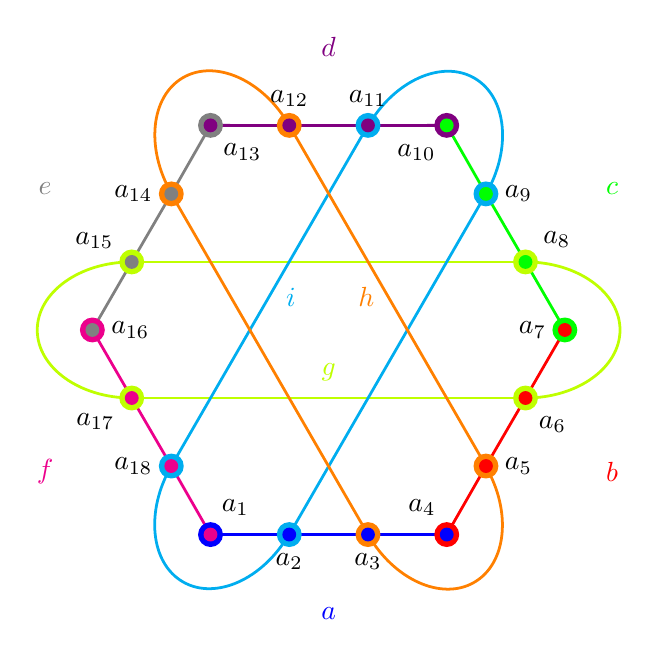
\begin{tikzpicture}  [scale=0.6]

		\tikzstyle{every path}=[line width=1pt]
		\tikzstyle{c2}=[circle,inner sep=3pt,minimum size=9pt]
		\tikzstyle{c1}=[circle,inner sep=0pt,minimum size=5pt]
		%\tikzstyle{s1}=[rectangle,minimum size=9]
		\tikzstyle{l1}=[draw=none,circle,minimum size=35]
		\tikzstyle{l2}=[draw=none,circle,minimum size=12]

		% Define positions of all observables
		\path
			  (240:5) coordinate(1)
			  (-0.833,-4.33) coordinate(2)
			  (0.833,-4.33) coordinate(3)
			  (300:5) coordinate(4)
			  (3.33,-2.88) coordinate(5)
			  (4.167,-1.44) coordinate(6)
     (0:5) coordinate(7)
			  (4.167,1.44) coordinate(8)
			  (3.33,2.88) coordinate(9)
		      (60:5) coordinate(10)
			  (0.833,4.33) coordinate(11)
			  (-0.833,4.33) coordinate(12)
			  (120:5) coordinate(13)
			  (-3.33,2.88) coordinate(14)
			  (-4.167,1.44) coordinate(15)
			  (180:5) coordinate(16)
			  (-4.167,-1.44) coordinate(17)
			  (-3.33,-2.88) coordinate(18);

\node[draw=none,color=blue] at (0,-6) {$a$};
\node[draw=none,color=red] at (6,-3) {$b$};
\node[draw=none,color=green] at (6,3) {$c$};
\node[draw=none,color=violet] at (0,6) {$d$};
\node[draw=none,color=gray] at (-6,3) {$e$};
\node[draw=none,color=magenta] at (-6,-3) {$f$};
\node[draw=none,color=cyan] at (-0.8,0.7) {$i$};
\node[draw=none,color=orange] at (0.8,0.7) {$h$};
\node[draw=none,color=lime] at (0,-0.9) {$g$};


	
		% Draw all the context curves
		\draw [color=green] (7) -- (8) -- (9)-- (10);
\draw [color=violet] (10) -- (11) -- (12) -- (13);
\draw [color=gray] (13) -- (14) -- (15) -- (16);
\draw [color=magenta] (16) -- (17) -- (18) -- (1);
\draw [color=blue] (1) -- (2) -- (3) -- (4);
\draw [color=red] (4) -- (5) -- (6) -- (7);

		\draw [color=lime] (8) -- (15);
		\draw [color=lime](17) -- (6);
		\draw [color=lime] (8) arc (450:270:2 and 1.44);
		\draw [color=lime] (15) arc (90:270:2 and 1.44);

		\draw [color=cyan] (9) -- (2);
		\draw [color=cyan] (11) -- (18);
		\draw [rotate=240,color=cyan] (9) arc (90:270:2 and 1.44);
		\draw[rotate=60,color=cyan] (18) arc (90:270:2 and 1.44);

		\draw [color=orange] (12) -- (5);
		\draw [color=orange] (14) -- (3);
		\draw[rotate=300,color=orange] (12) arc (90:270:2 and 1.44);
		\draw[rotate=120,color=orange] (3) arc (90:270:2 and 1.44);

		% Draw the observables themselves
		\draw (1) coordinate[c2,fill=blue];
		\draw (1) coordinate[c1,fill=magenta,label=85:$a_1$];
		\draw (2) coordinate[c2,fill=cyan];
		\draw (2) coordinate[c1,fill=blue,label=270:$a_2$];
\draw (3) coordinate[c2,fill=orange];
		\draw (3) coordinate[c1,fill=blue,label=270:$a_3$];
		\draw (4) coordinate[c2,fill=red];
		\draw (4) coordinate[c1,fill=blue,label=95:$a_4$];
\draw (5) coordinate[c2,fill=orange];
		\draw (5) coordinate[c1,fill=red,label=0:$a_5$];
\draw (6) coordinate[c2,fill=lime];
		\draw (6) coordinate[c1,fill=red,label=290:$a_6$];
		\draw (7) coordinate[c2,fill=green];
		\draw (7) coordinate[c1,fill=red,label=180:$a_7$];
\draw (8) coordinate[c2,fill=lime];
		\draw (8) coordinate[c1,fill=green,label=30:$a_8$];
\draw (9) coordinate[c2,fill=cyan];
		\draw (9) coordinate[c1,fill=green,label=0:$a_9$];
		\draw (10) coordinate[c2,fill=violet];
		\draw (10) coordinate[c1,fill=green,label=265:$a_{10}$];
\draw (11) coordinate[c2,fill=cyan];
		\draw (11) coordinate[c1,fill=violet,label=91:$a_{11}$];
\draw (12) coordinate[c2,fill=orange];
		\draw (12) coordinate[c1,fill=violet,label=90:$a_{12}$];
		\draw (13) coordinate[c2,fill=gray];
		\draw (13) coordinate[c1,fill=violet,label=285:$a_{13}$];
\draw (14) coordinate[c2,fill=orange];
		\draw (14) coordinate[c1,fill=gray,label=180:$a_{14}$];
\draw (15) coordinate[c2,fill=lime];
		\draw (15) coordinate[c1,fill=gray,label=160:$a_{15}$];
		%%\draw (15) node[c1,fill=none] {\Huge $\times$};
		%\draw (15) coordinate[s1,fill,label=150:$P_c$];
		%\draw (15) coordinate[c1,fill=white];
		%%\draw (15) coordinate[c1,draw];
		\draw (16) coordinate[c2,fill=magenta];
		\draw (16) coordinate[c1,fill=gray,label=0:$a_{16}$];
\draw (17) coordinate[c2,fill=lime];
		\draw (17) coordinate[c1,fill=magenta,label=215:$a_{17}$];
\draw (18) coordinate[c2,fill=cyan];
		\draw (18) coordinate[c1,fill=magenta,label=180:$a_{18}$];

		% Context labels
		%\coordinate[l1,label=260:$C_1$] (c1) at (16);
		%\coordinate[l2,label=25:$C_2$] (c2) at (16);
	\end{tikzpicture}
\end{center}
\caption{(Color online)
The most compact way of deriving the Kochen-Specker theorem in four dimensions has been given by
Cabello, Estebaranz and Garc{\'{i}}a-Alcaine~\cite{cabello-96}.
The configuration consists of 18 biconnected (two contexts intertwine per atom)
atoms $a_1, \ldots , a_{18}$ in 9 contexts.
It has a (quantum) realization in $\mathbb{R}^4$
consisting of the 18 projections associated with the one dimensional subspaces spanned by
the vectors from the origin $(0,0,0,0)^\intercal$ to
$a_1=\left(   0,0,1,-1     \right)^\intercal    $,
$a_2=\left(   1,-1,0,0     \right)^\intercal    $,
$a_3=\left(   1,1,-1,-1    \right)^\intercal   $,
$a_4=\left(   1,1,1,1      \right)^\intercal     $,
$a_5=\left(   1,-1,1,-1    \right)^\intercal  $,
$a_6=\left(   1,0,-1,0     \right)^\intercal   $,
$a_7=\left(   0,1,0,-1   \right)^\intercal   $,
$a_8=\left(   1,0,1,0    \right)^\intercal    $,
$a_9=\left(   1,1,-1,1   \right)^\intercal   $,
$a_{10}=\left(-1,1,1,1   \right)^\intercal    $,
$a_{11}=\left(1,1,1,-1   \right)^\intercal    $,
$a_{12}=\left(1,0,0,1    \right)^\intercal     $,
$a_{13}=\left(0,1,-1,0   \right)^\intercal    $,
$a_{14}=\left(0,1,1,0    \right)^\intercal    $,
$a_{15}=\left(0,0,0,1    \right)^\intercal    $,
$a_{16}=\left(1,0,0,0    \right)^\intercal    $,
$a_{17}=\left(0,1,0,0    \right)^\intercal    $,
$a_{18}=\left(0,0,1,1    \right)^\intercal    $,
 respectively~\cite[Fig.~1]{cabello:210401}
(for alternative realizations see Refs.~\cite{cabello-99,cabello:210401}).
%
\label{2016-pu-book-chapter-qm-f-kspac}
}
\end{figure}

In a parity proof by contradiction
consider the particular subset of real four-dimensional Hilbert space with a ``parity property,''
\index{parity property}
consisting of 18 atoms $a_1, \ldots , a_{18}$ in 9 contexts,
as depicted in Figure~\ref{2016-pu-book-chapter-qm-f-kspac}.
Note that, on the one hand,
each atom/point/vector/projector belongs
to exactly two -- that is, an {\em even} number of -- contexts; that is, it is biconnected.
Therefore,
%in order to obey non-contextuality -- in particular, the independence of any value of a two-valued state on the context it belongs to --
any enumeration of  all the contexts occurring in the graph
depicted in Figure~\ref{2016-pu-book-chapter-qm-f-kspac}
would contain an {\em even} number of $1$s assigned.
Because, due to non-contextuality and biconnectivity,
any atom $a$ with $v(a)=1$ along one context must have the same value 1 along the second context
which is intertwined with the first one -- to the values 1 appear in pairs.

Alas, on the other hand, in such an enumeration
there are nine  -- that is, an {\em odd} number of -- contexts.
Hence,
in order to obey the quantum predictions,
any  two-valued state (interpretable as truth assignment)
would need to have an {\em odd} number of $1$s -- exactly one for each context.
Therefore, there cannot exist any two-valued state on Kochen-Specker type graphs with the  ``parity property.''
%https://arxiv.org/pdf/1702.05215.pdf

More concretely,  note that, within each one of those 9 contexts,
the sum of any state on the atoms of that context must add up to 1.
That is, due to additivity (\ref{2017-ch-pu-qlff}) and (\ref{2017-ch-pu-glff})
one obtains a system of 9 equations
\begin{equation}
\begin{split}
\color{blue}        v(a)= v( a_1 ) + v( a_2 ) + v( a_3 ) + v( a_4 ) = 1 ,                  \\
\color{red}         v(b)= v( a_4 ) + v( a_5 ) + v( a_6 ) + v( a_7 ) = 1 ,                  \\
\color{green}       v(c)= v( a_7 ) + v( a_8 ) + v( a_9 ) + v( a_{10} ) = 1 ,               \\
\color{violet}      v(d)= v( a_{10} ) + v( a_{11} ) + v( a_{12} ) + v( a_{13} ) = 1 ,      \\
\color{gray}        v(e)= v( a_{13} ) + v( a_{14} ) + v( a_{15} ) + v( a_{16} ) = 1 ,      \\
\color{magenta}     v(f)= v( a_{16} ) + v( a_{17} ) + v( a_{18} ) + v( a_1 ) = 1 ,         \\
\color{lime}        v(g)= v( a_6 ) + v( a_8 ) + v( a_{15} ) + v( a_{17} ) = 1 ,            \\
\color{orange}      v(h)= v( a_3 ) + v( a_5 ) + v( a_{12} ) + v( a_{14} ) = 1 ,            \\
\color{cyan}        v(i)= v( a_2 ) + v( a_9 ) + v( a_{11} ) + v( a_{18} ) = 1 .
\label{2017-b-e-cabp-conf}
\end{split}
\end{equation}
By summing up the left hand side and the right hand sides of the equations, and since all atoms are biconnected,
one obtains
\begin{equation}
2 \left[\sum_{i=1}^{18} v(a_i)\right] = 9.
\label{2017-b-e-cabp}
\end{equation}
Because $v(a_i)\in \{0,1\}$ the sum in (\ref{2017-b-e-cabp}) must add up to some natural number $M$.
Therefore, Eq.~(\ref{2017-b-e-cabp}) is impossible to solve in the domain of natural numbers,
as on the left and right hand sides there appear even ($2M$) and odd ($9$) numbers, respectively.

Of course, one could also prove the nonexistence of any  two-valued state (interpretable as truth assignment)
by exhaustive attempts
(possibly exploiting symmetries) to assign values $0$s and $1$s to the atoms/points/vectors/projectors occurring in the graph
in such a way that both the quantum predictions as well as context independence is satisfied.
This latter method needs to be applied in cases with Kochen-Specker type diagrams without the  ``parity property;''
such as in the original Kochen-Specker proof~\cite{kochen1}.
(However, admissibility (IV) is too weak for a proof of this type,
as it allows also a third, value indefinte, state, which spoils the arguments~\cite{2015-AnalyticKS}.)

This result, as well as the original Kochen-Specker theorem,
is {\em state independent} insofar as it applies to an arbitrary quantum state.
One could {\em reduce the size of the proof} by assuming a particular state. Such proofs are called
{\em state-specific} or {\em state dependent.}
By following  Cabello, Estebaranz and Garc{\'{i}}a-Alcaine~\cite[Eqs.~(10)-(19), p.~185]{cabello-96}
their state independent proof utilizing the logic depicted in Fig.~\ref{2016-pu-book-chapter-qm-f-kspac}
can be transferred to a state-specific proof as follows:
suppose that the quantum (or quanta, depending upon the physical realization) is prepared in the state
\begin{equation}
v(a_1) = 1,
\label{2017-b-e-cabp2}
\end{equation}
so that any two-valued state must obey the admissibility rules
\begin{equation}
v(a_2)=v(a_3)=v(a_4)=v(a_{16}) =v(a_{17})=v(a_{18}) =0.
\label{2017-b-e-cabp3}
\end{equation}
The additivity relations~(\ref{2017-b-e-cabp-conf}) reduce to seven equations (two equations encoding contexts
${\color{blue}a}$ and ${\color{magenta}f}$ are satisfied trivially)
\begin{equation}
\begin{split}
\color{red}         v(b')=  v( a_5 ) + v( a_6 ) + v( a_7 ) = 1 ,                  \\
\color{green}       v(c)= v( a_7 ) + v( a_8 ) + v( a_9 ) + v( a_{10} ) = 1 ,               \\
\color{violet}      v(d)= v( a_{10} ) + v( a_{11} ) + v( a_{12} ) + v( a_{13} ) = 1 ,      \\
\color{gray}        v(e')= v( a_{13} ) + v( a_{14} ) + v( a_{15} ) = 1 ,      \\
\color{lime}        v(g')=  v( a_6 ) + v( a_8 ) + v( a_{15} ) = 1 ,            \\
\color{orange}      v(h')=  v( a_5 ) + v( a_{12} ) + v( a_{14} ) = 1 ,            \\
\color{cyan}        v(i')=  v( a_9 ) + v( a_{11} )  = 1 .
\label{2017-b-e-cabp-conf2}
\end{split}
\end{equation}
The configuration is depicted in Fig.~\ref{2016-pu-book-chapter-qm-f-kspac2}.
As all atoms remain to be biconnected and there are 7, that is,  an odd number, of equations, value
indefiniteness can be proven by a similar parity argument as before.
One could argue that the ``primed'' contexts in (\ref{2017-b-e-cabp-conf2}) are not complete
because those contexts are ``truncated.''
However, every completion would result in vectors orthogonal to $a_1$; and therefore their values must again be zero.
\begin{figure}
\begin{center}
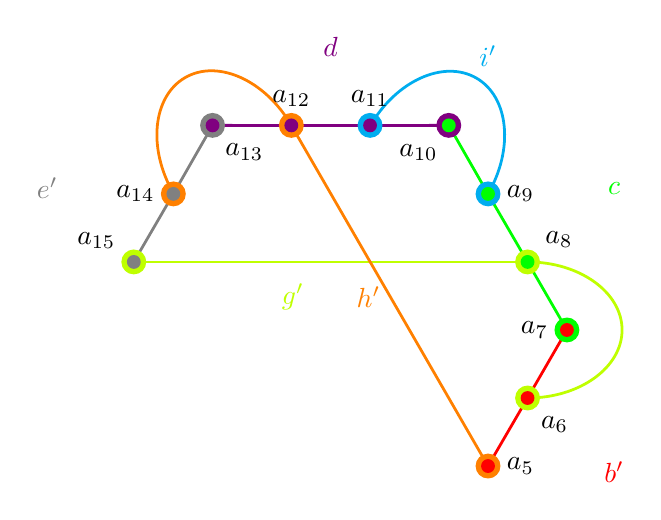
\begin{tikzpicture}  [scale=0.6]

		\tikzstyle{every path}=[line width=1pt]
		\tikzstyle{c2}=[circle,inner sep=3pt,minimum size=9pt]
		\tikzstyle{c1}=[circle,inner sep=0pt,minimum size=5pt]
		%\tikzstyle{s1}=[rectangle,minimum size=9]
		\tikzstyle{l1}=[draw=none,circle,minimum size=35]
		\tikzstyle{l2}=[draw=none,circle,minimum size=12]

		% Define positions of all observables
		\path
			  (3.33,-2.88) coordinate(5)
			  (4.167,-1.44) coordinate(6)
     (0:5) coordinate(7)
			  (4.167,1.44) coordinate(8)
			  (3.33,2.88) coordinate(9)
		      (60:5) coordinate(10)
			  (0.833,4.33) coordinate(11)
			  (-0.833,4.33) coordinate(12)
			  (120:5) coordinate(13)
			  (-3.33,2.88) coordinate(14)
			  (-4.167,1.44) coordinate(15);

%\node[draw=none,color=blue] at (0,-6) {$a$};
\node[draw=none,color=red] at (6,-3) {$b'$};
\node[draw=none,color=green] at (6,3) {$c$};
\node[draw=none,color=violet] at (0,6) {$d$};
\node[draw=none,color=gray] at (-6,3) {$e'$};
%\node[draw=none,color=magenta] at (-6,-3) {$f$};
\node[draw=none,color=cyan] at (3.33,5.8) {$i'$};
\node[draw=none,color=orange] at (0.8,0.7) {$h'$};
\node[draw=none,color=lime] at (-0.8,0.7) {$g'$};


	
		% Draw all the context curves
		\draw [color=green] (7) -- (8) -- (9)-- (10);
\draw [color=violet] (10) -- (11) -- (12) -- (13);
\draw [color=gray] (13) -- (14) -- (15) ;
%\draw [color=magenta] (16) -- (17) -- (18) -- (1);
%\draw [color=blue] (1) -- (2) -- (3) -- (4);
\draw [color=red] (5) -- (6) -- (7);

  \draw [color=lime] (8) -- (15);
%	\draw [color=lime](17) -- (6);
		\draw [color=lime] (8) arc (450:270:2 and 1.44);
%	\draw [color=lime] (15) arc (90:270:2 and 1.44);

%		\draw [color=cyan] (9) -- (2);
%		\draw [color=cyan] (11) -- (18);
  	\draw [rotate=240,color=cyan] (9) arc (90:270:2 and 1.44);
%		\draw[rotate=60,color=cyan] (18) arc (90:270:2 and 1.44);

		\draw [color=orange] (12) -- (5);
%	\draw [color=orange] (14) -- (3);
		\draw[rotate=300,color=orange] (12) arc (90:270:2 and 1.44);
%	\draw[rotate=120,color=orange] (3) arc (90:270:2 and 1.44);

		% Draw the observables themselves
\draw (5) coordinate[c2,fill=orange];
		\draw (5) coordinate[c1,fill=red,label=0:$a_5$];
\draw (6) coordinate[c2,fill=lime];
		\draw (6) coordinate[c1,fill=red,label=290:$a_6$];
		\draw (7) coordinate[c2,fill=green];
		\draw (7) coordinate[c1,fill=red,label=180:$a_7$];
\draw (8) coordinate[c2,fill=lime];
		\draw (8) coordinate[c1,fill=green,label=30:$a_8$];
\draw (9) coordinate[c2,fill=cyan];
		\draw (9) coordinate[c1,fill=green,label=0:$a_9$];
		\draw (10) coordinate[c2,fill=violet];
		\draw (10) coordinate[c1,fill=green,label=265:$a_{10}$];
\draw (11) coordinate[c2,fill=cyan];
		\draw (11) coordinate[c1,fill=violet,label=91:$a_{11}$];
\draw (12) coordinate[c2,fill=orange];
		\draw (12) coordinate[c1,fill=violet,label=90:$a_{12}$];
		\draw (13) coordinate[c2,fill=gray];
		\draw (13) coordinate[c1,fill=violet,label=285:$a_{13}$];
\draw (14) coordinate[c2,fill=orange];
		\draw (14) coordinate[c1,fill=gray,label=180:$a_{14}$];
\draw (15) coordinate[c2,fill=lime];
		\draw (15) coordinate[c1,fill=gray,label=160:$a_{15}$];
		%%\draw (15) node[c1,fill=none] {\Huge $\times$};
		%\draw (15) coordinate[s1,fill,label=150:$P_c$];
		%\draw (15) coordinate[c1,fill=white];
		%%\draw (15) coordinate[c1,draw];

		% Context labels
		%\coordinate[l1,label=260:$C_1$] (c1) at (16);
		%\coordinate[l2,label=25:$C_2$] (c2) at (16);
	\end{tikzpicture}
\end{center}
\caption{(Color online)
Greechie orthogonality diagram of a state-specific proof of the Kochen-Specker theorem
based on the assumption that the physical system is  in state $a_1$, such that $v(a_1)=1$.
The additivity and admissibility constraints  (\ref{2017-b-e-cabp-conf2}) represent different ``reduced'' (or ``truncated'') contexts,
because all states $v(a_2)=v(a_3)=v(a_4)=v(a_{16}) =v(a_{17})=v(a_{18}) =0$ ``orthogonal to'' $a_1$ must vanish.
\label{2016-pu-book-chapter-qm-f-kspac2}
}
\end{figure}



\subsubsection*{Chromatic number of the sphere}

Graph coloring allows another view on value (in)definiteness.
The {\em chromatic number} of a graph
\index{chromatic number}
is defined as the least number of colors needed in any total coloring of a graph;
with the constraint that two adjacent vertices have distinct colors.

Suppose that we are interested in the chromatic number of graphs associated with
both (i) the real and (ii) the rational three-dimensional unit sphere.
%defined by
%$S^3 =
%\big\{ \vert {\bf x} \rangle \big|  \vert {\bf x} \rangle =
%\begin{pmatrix}
%x_1,x_2,x_3
%\end{pmatrix}^\intercal
%, \;
%x_1^2+x_2^2+x_3^2=1, \; x_1,x_2,x_3 \in \mathbb{R}
%\big\}
%$,
%as well as $S^3\cap \mathbb{Q}^3$, respectively.

More generally, we can consider $n$-dimensional unit spheres with the same adjacency property defined by orthogonality.
An orthonormal basis will be called context (block, maximal observable, Boolean subalgebra),
or, in this particular area, a $n$-clique.
Note that for any such graphs involving $n$-cliques the chromatic number of this graph is at least be $n$
(because the chromatic number of a single $n$-clique or context is $n$).

Thereby vertices of the graph are identified with points on the three-dimensional unit sphere;
with adjacency  defined by orthogonality; that is,
two vertices of the graph are adjacent if and only if the unit vectors from the origin
to the respective two points are orthogonal.

The connection to quantum logic is this: any context
(block, maximal observable, Boolean subalgebra, orthonormal basis)
can be represented by a triple of points on the sphere
such that any two unit vectors from the origin
to two distinct points of that triple of points are orthogonal.
Thus graph adjacency in logical terms indicates
``belonging to some common context (block, maximal observable, Boolean subalgebra, orthonormal basis).''

In three dimensions, if the chromatic number of  graphs is four or higher,
there does not globally exist any consistent
coloring obeying the rule that adjacent vertices (orthogonal vectors)
must have different colors: if one allows only three different colors,
then somewhere in that graph of chromatic number higher than three, adjacent vertices must have the same colors
(or else the chromatic number would be three or lower).


By a similar argument, non-separability of two-valued states
--
such as encountered in Section~\ref{2017-b-bugscombino}
with the $\Gamma_3$-configuration of Kochen-Specker~\cite[p.~70]{kochen1}
-- translates into non-differentiability by colorings
with colors less or equal to the number of atoms in a block
(cf. Fig.~\ref{2017-b-f-twobugschromaticsep}).

Godsil and Zaks~\cite{godsil-zaks,havlicek-2000}  proved the following results:
\begin{enumerate}
\item
the chromatic number of the graph based on points of real-valued unit sphere
is four~\cite[Lemma~1.1]{godsil-zaks}.
\item
The chromatic number of rational points on the  unit sphere
$S^3\cap \mathbb{Q}^3$
is three~\cite[Lemma~1.2]{godsil-zaks}.
\end{enumerate}

We shall concentrate on (i) and discuss (ii) later.
As has been pointed out by Godsil in an email conversation from March 13, 2016~\cite{godsil-pc},
{\em ``the fact that the chromatic number of the unit sphere in $\mathbb{R}^3$
is four is a consequence of  Gleason's theorem,
from which the Kochen-Specker theorem follows by compactness.
Gleason's result implies that there is no subset of the sphere that contains exactly one point from each orthonormal basis.''}

Indeed, any coloring can be mapped onto a two-valued state by identifying
a single color with ``$1$'' and all other colors with ``$0$.''
By reduction, all propositions on two-valued states translate into statements about graph coloring.
In particular, if the chromatic number of any logical structure representable as graph consisting of $n$-atomic
contexts
(blocks, maximal observables with $n$ outcomes, Boolean subalgebras $2^n$, orthonormal bases with $n$ elements)
--
for instance, as Greechie orthogonality diagram of quantum logics
--
is larger than $n$,
then there cannot be any globally consistent two-valued state (truth value assignment) obeying adjacency (aka admissibility).
Likewise, if no two-valued states  on a logic
which is a pasting of $n$-atomic contexts
exist, then, by reduction, no global consistent coloring with $n$ different colors exists.
Therefore, the Kochen-Specker theorem proves that the chromatic number of the graph corresponding to
the unit sphere with adjacency defined as orthogonality must be higher than three.




%\subsubsection*{Breaking up intertwines}

Based on Godsil and Zaks finding that the chromatic number of rational points on the  unit sphere
$S^3\cap \mathbb{Q}^3$
is three~\cite[Lemma~1.2]{godsil-zaks} -- thereby constructing a two-valued measure on the rational unit sphere
by identifying one color with ``$1$'' and the two remaining colors with ``$0$'' --
there exist ``exotic'' options to circumvent Kochen-Specker type constructions which have been quite aggressively (Cabello has referred to this
as the {\em second contextuality war} \cite{Cabello-talk-Vajo-2017})
marketed by allegedly ``nullifying''~\cite{meyer:99} the respective theorems
under the umbrella of ``finite precision measurements''~\cite{kent:99,clifton:99,mermin-99iks,Breuer-02a,Breuer-02b,Barrett-2004}:
the support of vectors spanning the one-dimensional subspaces associated with atomic propositions could be ``diluted'' yet dense,
so much so that the intertwines of contexts (blocks, maximal observables, Boolean subalgebras, orthonormal bases) break up;
and the contexts themselves become ``free \& isolated.''
Under such circumstances the logics decay into horizontal sums;
and the Greechie orthogonality diagrams are just disconnected stacks of previously intertwined contexts.
As can be expected, proofs of Gleason- or Kochen-Specker-type theorems do no longer exist,
as the necessary intertwines are missing.

%More concretely,
%one could consider all unit vectors with the
%{\em Pythagorean property}
%$i^2+j^2+k^2=n^2$ for $i,j,k \in \mathbb{Z}, n \in \mathbb{N}$;
%that is,
%\begin{equation}
%\begin{split}
%\Big\{ \vert {\bf x} \rangle \Big|  \vert {\bf x} \rangle =
%\begin{pmatrix}
%\frac{i}{n},\frac{j}{n},\frac{k}{n}
%\end{pmatrix}^\intercal
%,
%i,j,k,n \in \mathbb{Z} \setminus \left\{\left(0,0,0\right)^\intercal \right\}, \\
%i^2+j^2+k^2=n^2
%\Big\}  = S^3\cap \mathbb{Q}^3
%\end{split}
%\end{equation}
%encodes all rational points
%on the unit sphere.
%This can be verified by writing any rational point on the unit sphere as
%$   \vert {\bf r} \rangle =
%\begin{pmatrix}
%\frac{a}{a'},\frac{b}{b'},\frac{c}{c'}
%\end{pmatrix}^\intercal
%$  with
%$a,b,c\in \mathbb{Z}$ and
%$a',b',c'\in \mathbb{Z} \setminus \left\{ 0 \right\}$,
%with
%$
%\left(\frac{a}{a'}\right)^2 + \left(\frac{b}{b'}\right)^2 + \left(\frac{c}{c'}\right)^2 =1
%$.
%Multiplying $\vert {\bf r} \rangle$  with
%with ${a'}{b'}{c'}$
%yields a vector satisfying the Pythagorean property
%$
%({a }{b'}{c'})^2 +
%({a'}{b }{c'})^2 +
%({a'}{b'}{c })^2=
%({a'}{b'}{c'})^2
%$.

The ``nullification'' claim and subsequent ones triggered a lot of papers, some cited in ~\cite{Barrett-2004};
mostly critical -- of course, not to the results of Godsil and Zaks's finding (ii); how could they? -- but to their physical applicability.
Peres even wrote a parody by arguing that  {\em ``finite precision measurement nullifies Euclid's postulates''}~\cite{peres-2003-fpnep},
so that ``nullification'' of the Kochen-Specker theorem might have to be our least concern.
%Rather than presenting a detailed formal discussion I shall mention an anecdote: shortly after
%the publication of ``nullification'' paper~\cite{meyer:99} Specker called me up in Vienna.
%He was quite upset and suggested
%(in German; translated from my memory):
%{\em ``I need not be directly involved in this; but you should write a response to that paper.''}
%
%So I conceived a reply (now partially contained in~\cite{havlicek-2000}) --
%basically criticising that, in such a configuration, every neighborhood of points on the sphere
%would have to be colored with all three colors; and thus, by identification, the resulting probability measure (frame function)
%would be highly discontinuous -- a discontinuity which is not encountered in actual experiment;
%as well as the absence of closedness under fundamental logical processes.
%
%After councellation with Specker we submitted a comment
%which met the highest resistance in the peer review processes of two journals ({\em Physical Review Letters} and {\em Physics Letters A})
%which rejected the manuscript.
%One referee pointed out that {\em ``the usual meaning of the phrase ``Kochen-Specker
%        theorem'' is not quite what the authors state''}
%(thereby basically unknowingly alleging that Specker did not know what his own theorem was about).
%Another, final, referee  remarked that
%{\em ``the authors' first criticism of Meyer seems to me perverse.''}

%Specker's typical reaction in a personal email messages from June 20th, 2000~\cite{Specker-priv-June2000},
%with reference to~\cite{clifton:99},
%was,
%{\em that a dense set $M$ of directions exist in $n$-dimensional space with the property that
%no two directions in $M$ are orthogonal, that is completely evident (assuming some familiarity
%in topology and recursive constructions).
%Of course, for such directions no problems exist with regards to imbedability.
%If that appears too trivial, a dense set of directions can be constructed such that every direction
%belongs to exactly one basis.''}~\footnote{
%{G}erman original:
%{\em ``Dass es eine dichte Menge M von Richtungen
%im n-dimensionalen Raum (oder auch im Hilbertraum) gibt mit der Eigenschaft,
%dass keine zwei Richtungen in M orthogonal sind, das ist nun wirklich ganz
%selbstverst\"andlich (vorausgesetzt nat\"urlich einig Vertrautheit mit Topologie
%und rekursiven Konstruktionen). F\"ur solche Richtungen besteht dann nat\"urich
%\"uberhaupt kein Problem der Einbettbarkeit. Ist das allzu trivial, so kann
%auch eine dichte Menge von Richtungen konstruiert werden, so dass jede
%Richtung zu genau einer Basis geh\"ort.''}}
%Referring to his personal experiences with peer reviews, Specker remarked,
%{\em ``I am sorry that you have so many trouble with your work --
%it might be a little bit consoling for you that I have made the same experiences in this area.

%I am not surprised -- as I have occasionally suggested the area is
%(at least as far as I am concerned) haunted -- and I have convinced myself
%a couple of times that I contribute only ``preachingwise'' --
%that is, it is implicitly settled that one speaks and the others remain silent.
%Under such circumstances publications are almost excluded.''}\footnote{
%{G}erman original:
%{\em ``
%es tut mir leid, dass ihr mit eurer Arbeit soviel \"Arger habt - vielleicht
%tr\"ostet es dich ja eine wenig, dass es mir auf diesem Gebiet auch nicht viel
%anders ergangen ist.
%
%Ueberrascht bin ich nicht - wie ich ja gelegentlich andeute, ist das Gebiet
%(wenigstens was mich betrifft) verhext - und ich habe mir schon mehrmals
%vorgenommen, mich nur noch ``predigenderweise'' zu beteiligen - d.h. es ist
%stillchweigend abgemacht, dass der eine redet und die andern schweigen.
%Publikationen sind da fast ausgeschlossen.''}.}
%One of the reasons for the kind of hauntedness experienced by Specker and
%others~\cite{clauser-talkvie} might be the evangelical furor by
%which some protagonists pursue their visions of (in)determinism.




\subsubsection*{Exploring value indefiniteness}
\label{2017-b-c-eokst}

Maybe one could, with all due respect,
speak of ``extensions'' of the Kochen-Specker theorem by looking at situations
in which a system is prepared in a state
$\vert {\bf x} \rangle \langle {\bf x} \vert$  along direction
$\vert {\bf x} \rangle$
and measured along a non-orthogonal, non-collinear projection
$\vert {\bf y} \rangle \langle {\bf y} \vert$  along direction
$\vert {\bf y} \rangle$.
Those extensions yield what may be called~\cite{pitowsky:218,hru-pit-2003} {\em indeterminacy}.
Indeterminacy may be just another word for {\em contextuality};
but, as has been suggested by the realist Bell,
the latter term implicitly implies that
there ``is something (rather than nothing) out there,'' some ``pre-existing observable''
which, however, needs to depend on the context of the measurement.
To avoid such implicit assumption we shall henceforth use  indeterminacy rather than contextuality.

Pitowsky's  {\em logical indeterminacy principle}~\cite[Theorem~6, p.~226]{pitowsky:218}
states that, given two linearly independent
non-orthogonal unit vectors
$\vert {\bf x} \rangle$
and
$\vert {\bf y} \rangle$
in $\mathbb{R}^3$,
there is a finite set of unit vectors
$\Gamma ( \vert {\bf x} \rangle , \vert {\bf y} \rangle )$ containing
$\vert {\bf x} \rangle$
and
$\vert {\bf y} \rangle$
for which the following statements hold:
\begin{enumerate}
\item
There is no (not necessarily two-valued) state $v$ on $\Gamma ( \vert {\bf x} \rangle , \vert {\bf y} \rangle )$ which
satisfies
$v ( \vert {\bf x} \rangle ) = v ( \vert {\bf y} \rangle ) =1$.
\item
There is no (not necessarily two-valued)  $v$ on $\Gamma ( \vert {\bf x} \rangle , \vert {\bf y} \rangle )$
which satisfies $v ( \vert {\bf x} \rangle ) = 1$ and $ v ( \vert {\bf y} \rangle ) =0$.
\item
There is no (not necessarily two-valued)  state $v$ on $\Gamma ( \vert {\bf x} \rangle , \vert {\bf y} \rangle )$
which satisfies $v ( \vert {\bf x} \rangle ) = 0$ and $ v ( \vert {\bf y} \rangle ) =1$.
\end{enumerate}

Stated differently~\cite[Theorem~2,p~183]{hru-pit-2003},
let $\vert {\bf x} \rangle$
and
$\vert {\bf y} \rangle$
be two non-orthogonal rays in a Hilbert space $\mathfrak{H}$ of finite
dimension $\ge 3$. Then there is a finite set of rays $\Gamma ( \vert {\bf x} \rangle , \vert {\bf y} \rangle )$ containing
$\vert {\bf x} \rangle$
and
$\vert {\bf y} \rangle$
such that a (not necessarily two-valued)
state $v$ on $\Gamma ( \vert {\bf x} \rangle , \vert {\bf y} \rangle )$
satisfies $v ( \vert {\bf x} \rangle ),( \vert {\bf y} \rangle ) \in \{0,1\}$
only if $v ( \vert {\bf x} \rangle ) = v ( \vert {\bf y} \rangle ) =0$.
That is,
if a system of three mutually exclusive outcomes (such as the spin of a spin-$1$ particle in a particular direction)
is prepared in a definite state $\vert {\bf x} \rangle$  corresponding to $v(\vert {\bf x} \rangle )=1$,
then the state $ v ( \vert {\bf y} \rangle ) $ along  some direction $\vert {\bf y} \rangle $ which is neither collinear nor orthogonal
to  $\vert {\bf x} \rangle$
cannot be (pre-)determined,
because, by an argument {\it via} some set of intertwined rays  $\Gamma ( \vert {\bf x} \rangle , \vert {\bf y} \rangle )$,
both cases would lead to a complete contradiction.

The proofs of the logical indeterminacy principle
presented by  Pitowsky and Hrushovski~\cite{pitowsky:218,hru-pit-2003}
is global in the sense that any ray in the
set of intertwining rays $\Gamma ( \vert {\bf x} \rangle , \vert {\bf y} \rangle )$
in-between  $\vert {\bf x} \rangle$
and
$\vert {\bf y} \rangle$  -- and thus not necessarily the ``beginning and end points''
$\vert {\bf x} \rangle$
and
$\vert {\bf y} \rangle$
--
may not have a pre-existing value.
(If you are an omni-realist, substitute ``pre-existing'' by ``non-contextual:''
that is, any ray in the
set of intertwining rays $\Gamma ( \vert {\bf x} \rangle , \vert {\bf y} \rangle )$
may violate the admissibility rules and, in particular, non-contextuality.)
Therefore, one might argue that the cases
(i) as well as (ii); that is,
$v ( \vert {\bf x} \rangle ) = v ( \vert {\bf y} \rangle ) =1$.
as well as
$v ( \vert {\bf x} \rangle ) = 1$ and $ v ( \vert {\bf y} \rangle ) =0$
might still be predefined, whereas at least one ray in $\Gamma ( \vert {\bf x} \rangle , \vert {\bf y} \rangle )$ cannot be pre-defined.
(If you are an omni-realist, substitute ``pre-defined'' by ``non-contextual.'')


This possibility  has been excluded in a series of papers~\cite{Abbott:2010uq,2012-incomput-proofsCJ,PhysRevA.89.032109,2015-AnalyticKS}
{\em localizing value indefiniteness}.
Thereby the strong admissibility rules coinciding with two-valued states which are total function on a logic, have been generalized or extended (if you prefer ``weakened'')
in such away as to allow for value definiteness.
Essentially, by allowing the two-valued state to be a {\em partial} function on the logic,
which need not be defined any longer on all of its elements,
admissability has been defined by two rules (IV) of Section~\ref{2017-b-admissability}:
if $v ( \vert {\bf x} \rangle ) = 1$, then a measurement of all the other observables in a context  containing $\vert {\bf x} \rangle$  must yield
the value  $0$  for the other observables in this
context -- as well as counterfactually, in all contexts including $\vert {\bf x} \rangle$ and in mutually orthogonal rays which are orthogonal to $\vert {\bf x} \rangle$,
such as depicted as the star-shaped configuration in Fig.~\ref{2017-b-c-notvsstar}.
Likewise, if all propositions but one, say the one associated with $\vert {\bf x} \rangle$, in a context have value $0$, then this proposition $\vert {\bf x} \rangle$
is assigned the value $1$; that is,  $v ( \vert {\bf x} \rangle ) = 1$.

However,
as long as the entire context contains more than two atoms,
if  $v ( \vert {\bf x} \rangle ) = 0$ for some proposition associated with $\vert {\bf x} \rangle $,
%even though measurement of $\vert {\bf x} \rangle$ must yield the outcome $0$,  then,
any of the other observables in the context containing $\vert {\bf x} \rangle$ could
still yield the value $1$ or $0$.
Therefore, these other observables need not be  value definite.
In such a formalism, and relative to the assumptions -- in particular,
by the admissibility rules allowing for value indefiniteness
--
sets of intertwined rays  $\Gamma ( \vert {\bf x} \rangle , \vert {\bf y} \rangle )$
can be constructed
which render value indefiniteness of property $\vert {\bf y} \rangle  \langle {\bf y} \vert $
if the system is prepared in state $\vert {\bf x} \rangle$ (and thus $ v( \vert {\bf x} \rangle )=1$).
More specifically,
sets of intertwined rays  $\Gamma ( \vert {\bf x} \rangle , \vert {\bf y} \rangle )$
can be found which demonstrate that, in accord with the ``weak'' admissibility rules (IV)
of Section~\ref{2017-b-admissability},
in Hilbert spaces of dimension greater than two,
in accord with complementarity,
any proposition which is complementary with respect to the state prepared
must be value indefinite ~\cite{Abbott:2010uq,2012-incomput-proofsCJ,PhysRevA.89.032109,2015-AnalyticKS}.


\subsubsection*{How can you measure a contradiction?}

Clifton replied with this (rhetorical) question
%on a bus to Prague's city center,
%where the conference dinner  of the biannual meeting of the second biennial conference of
%{\em International Quantum Structure Association} took place in the late summer of 1994.
after I had asked if he could imagine any possibility to somehow ``operationalize'' the Kochen-Specker theorem.

Indeed, the Kochen-Specker theorem -- in particular, not only non-separability but the total absence of any two-valued state --
has been resilient to attempts to somehow ``measure'' it:
first, as alluded by Clifton, its proof is by contraction --
any assumption or attempt to consistently (in accordance with admissibility)
construct two-valued state on certain finite subsets of quantum logics provably fails.

Second, the very absence of any two-valued state on such logics reveals the futility of any attempt to somehow define classical probabilities;
let alone the derivation of any Boole's conditions of physical experience --
both rely on, or are,  the hull spanned by the vertices derivable from two-valued states (if the latter existed) and the respective correlations.
So, in essence, on logics corresponding to Kochen-Specker configurations, such as
the $\Gamma_2$-configuration of Kochen-Specker~\cite[p.~69]{kochen1}, or
the Cabello, Estebaranz and Garc{\'{i}}a-Alcaine logic~\cite{cabello-96,cabello-99}
depicted in Fig.~\ref{2016-pu-book-chapter-qm-f-kspac}
which (subject to admissibility) have no two-valued states,
classical probability theory breaks down entirely -- that is, in the most fundamental way;
by not allowing any two-valued state.



It is amazing how many papers exist which claim to ``experimentally verify'' the Kochen-Specker theorem.
However, without exception, those experiments either prove some kind of Bell-Boole of inequality
on single-particles (to be fair this is referred to as ``proving contextuality;''
such as, for instance, Refs.~\cite{Hasegawa-2003,hasegawa:230401,cabelloFilipp-2008,Bartosik-09,kirch-09});
or show that the quantum predictions yield complete contradictions if  one ``forces'' or assumes the counterfactual
co-existence of
observables in different contexts (and measured in separate, distinct experiments carried out in different subensembles; e.g.,
Refs.~\cite{ghz,cabello-99,Si-Zu-Wein-Ze-2000,panbdwz,simon-2002};
again these lists of references are incomplete.)

Of course, what one could still do is measuring all contexts, or subsets of compatible observables
(possibly by Einstein-Podolsky-Rosen type~\cite{epr} counterfactual inference) -- one at a time --
 on different subensembles
prepared in the same state by Einstein-Podolsky-Rosen type~\cite{epr} experiments,
and comparing the complete sets of results
with classical predictions~\cite{ghz}.
For instance, multiplying all products  of dichotomic $\pm 1$ observables within contexts,
and summing up the results in
parity proofs such as for the Cabello, Estebaranz and Garc{\'{i}}a-Alcaine logic
depicted in Fig.~ref{2016-pu-book-chapter-qm-f-kspac}
must yield differences between the classical and the quantum predictions --
in this case parity odd and even, respectively.

\subsubsection*{Contextual inequalities}

If one is willing to drop admissibility altogether while at the same time maintaining non-contextuality -- thereby only assuming
that the hidden variable theories assign
values to all the observables~\cite[Sect.~4, p.~375]{Bengtsson-2012},
thereby  only assuming non-contextuality~\cite{cabello:210401},
one arrives at {\em contextual inequalities}~\cite{cabello-2013-ncyclea}.
Of course, these value assignments need to be much more general as the admissibility requirements on
two-valued states; allowing all $2^n$ (instead of just $n$ combinations) of contexts with $n$ atoms;
such as $1-1-1- \ldots -1$, or $0-0-\ldots -0$.
For example, Cabello has suggested~\cite{cabello:210401} to consider fourth order correlations within all the contexts
(blocks; really within single maximal observables)
constituting the logic considered by
Cabello, Estebaranz and Garc{\'{i}}a-Alcaine~\cite{cabello-96,cabello-99},
and depicted as a Greechie orthogonality diagram in Fig.~\ref{2016-pu-book-chapter-qm-f-kspac}.
For the sake of demonstration, consider a Greechie (orthogonality) diagram of a
finite subset of the continuum of blocks or contexts imbeddable in
four-dimensional real Hilbert space without a two-valued probability measure.
More explicitly, the correlations are with  nine tightly interconnected contexts
$\color{blue}a=\{a_1,a_2,a_3,a_4\}$,
$\color{red}b=\{a_4,a_5,a_6,a_7\}$,
$\color{green}c=\{a_7,a_8,a_9,a_{10}\}$,
$\color{violet}d=\{a_{10},a_{11},a_{12},a_{13}\}$,
$\color{gray}e=\{a_{13},a_{14},a_{15},a_{16}\}$,
$\color{magenta}f=\{a_{16},a_{17},a_{18},a_1\}$,
$\color{lime}g=\{a_6,a_8,a_{15},a_{17}\}$
$\color{orange}h=\{a_3,a_5,a_{12},a_{14}\}$,
$\color{cyan}i=\{a_2,a_9,a_{11},a_{18}\}$, respectively.

A hull problem can be defined as follows:
(i) assume that each one of the 18 (partially counterfactual) observables
$a_1,a_2, \ldots ,a_{18}$ independently acquires either the definite value
``$-1$''
or
``$+1$,'' respectively.
There are $2^{18}=262144$ such cases. Note that, essentially, thereby all information on the intertwine structure is eliminated
(the only remains are in the correlations taken in the next step),
as one treats all observables to belong to a large Boolean algebra of 18 atoms  $a_1,a_2, \ldots ,a_{18}$;
(ii) form all the 9 four-order correlations according to the context (block) structure
${\color{blue}a_1 a_2 a_3 a_4}, {\color{red}a_4 a_5 a_6 a_7}, \ldots , {\color{cyan}a_2 a_9 a_{11} a_{18}}$, respectively;
(iii) then evaluate (by multiplication) each one of these nine observables according to the valuations created in (i);
(iv) for each one of the $2^{18}$ valuations form a 9-dimensional vector
$\left( E_1 ={\color{blue}a_1 a_2 a_3 a_4}, E_2={\color{red}a_4 a_5 a_6 a_7}, \ldots , E_9={\color{cyan}a_2 a_9 a_{11} a_{18}}\right)^\intercal$
which contains all the values computed in (iii),
and consider them as vertices (of course, there will be many duplicates which can be eliminated) defining a correlation polytope;
(v) finally, solve the hull problem for this polytope.
The resulting 274 inequalities and 256 vertices (a reverse vertex computation reveals 256 vertices; down from $2^{18}$)
confirms  Cabello's~\cite{cabello:210401}
as well as other bounds~\cite[Eqs.~(8)]{svozil-2016-s}; among them
\begin{equation}
\begin{split}
-1 \leq  E_1 \leq 1, \\
E_1+7\geq E_2+E_3+E_4+E_5+E_6+E_7+E_8+E_9, \\
E_1+E_8+E_9+7\geq E_2+E_3+E_4+E_5+E_6+E_7, \\
E_1+E_6+E_7+E_8+E_9+7\geq E_2+E_3+E_4+E_5, \\
E_1+E_4+E_5+E_6+E_7+E_8+E_9+7\geq E_2+E_3, \\
E_1+E_2+E_3+E_4+E_5+E_6+E_7+E_8+E_9+7\geq 0
.
\end{split}
\label{2015-s-e11}
\end{equation}

Similar calculations for the pentagon and the Specker bug logics,
by ``bundling'' the 3rd order correlations within the contexts (blocks, 3-atomic Boolean subalgebras), yield
$32$
(down from $2^{10}=1024$ partially duplicate)
vertices and 10 ``trivial'' inequalities for the bug logic,
as well as 128
(down from $2^{13}=8192$ partially duplicate)
vertices and 14 ``trivial'' inequalities for the Specker bug logic.


\subsection{Quantum probabilities and expectations}

Since from Hilbert space dimension higher than two there do not exist any two-valued states,
the (quasi-)classical Boolean strategy to find (or define) probabilities {\it via}
the convex sum of two-valued states brakes down entirely.
Therefore, as this happened to be~\cite{Dirac621,dirac,Jordan1927,vonNeumann:1927:WAQ,v-neumann-49,v-neumann-55},
the quantum probabilities have to be ``derived'' or postulated from
entirely new concepts, based upon quantities -- such as vectors or projection operators --
in linear vector spaces equipped with a scalar product.
One guiding principle should be that, among those observables which are simultaneously co-measurable (that is, whose
projection operators commute), the classical probability theory should hold.

Historically, what is often referred to as
{\em Born rule}
\index{Born rule}
for calculating probabilities,
has been a statistical re-interpretation of Schr\"odinger's
wave function~\cite[Footnote 1, Anmerkung bei der Korrektur, p.~865]{born-26-1},
as outlined by Dirac~\cite{Dirac621,dirac}
(a digression: a small piece~\cite{dirac-81} on {\em ``the futility of war''}
by the late Dirac is highly recommended; I had the honour listening to the talk personally), Jordan~\cite{Jordan1927},
von Neumann~\cite{vonNeumann:1927:WAQ,v-neumann-49,v-neumann-55}, and
L\"uders~\cite{Luders-1950,Luders-1950e,Busch2009}.

Rather than stating it as axiom of quantum mechanics,
Gleason~\cite{Gleason}
derived the Born rule from elementary assumptions; in particular from subclassicality: within contexts -- that is,
among mutually commuting and thus simultaneously co-measurable observables -- the
quantum probabilities should reduce to the classical, Kolmogorovian, form.
In particular, the probabilities of propositions corresponding to observables which are (i) mutually exclusive
(in geometric terms: correspond to orthogonal vectors/projectors)
as well as (ii) simultaneously co-measurable observables
are (i) non-negative, (ii) normalized, and (iii) finite additive as in
Eqs.~(\ref{2017-ch-pu-qlff}) and~(\ref{2017-ch-pu-glff}); that is, probabilities
(of atoms within contexts or blocks)
add up to one~\cite[Section~1]{sep-probability-interpret}.

As already mentioned earlier, Gleason's paper made a high impact on those in the community capable
of comprehending it~\cite{ZirlSchl-65,kamber65,bell-66,kochen1,c-k-m,r:dvur-93,pitowsky:218,rich-bridge}.
Nevertheless it might not be unreasonable to state that, while a proof of the Kochen-Specker theorem is straightforward,
Gleason's results are less attainable.
However, in what follows we shall be less concerned with either necessity nor with mixed states,
but shall rather concentrate on sufficiency and pure states.
(This will also rid us of the limitations to Hilbert spaces of dimensions higher that two.)

Recall that pure states~\cite{Dirac621,dirac}
as well as elementary yes-no propositions~\cite{v-neumann-49,v-neumann-55,birkhoff-36} can both
be represented by (normalized) vectors in some Hilbert space.
If one prepares a pure state corresponding to a unit vector
$\vert {\bf x} \rangle$ (associated with the one-dimensional projection operator
$\textsf{\textbf{E}}_{\bf x}=\vert {\bf x} \rangle \langle {\bf x} \vert $)
and measures an elementary yes-no proposition, representable by a one-dimensional projection operator
$\textsf{\textbf{E}}_{\bf y}=\vert {\bf y} \rangle \langle {\bf y} \vert $
(associated with the vector
$\vert {\bf y} \rangle$),
then Gleason notes~\cite[p.~885]{Gleason} in the second paragraph that (in Dirac notation),
{\em  ``it is easy to see that such a [[probability]] measure $\mu$
%[[satisfying subadditivity]]
can be obtained by selecting a vector $\vert {\bf y} \rangle$
and, for each closed subspace $A$, taking $\mu ({A})$ as the square of the norm of the
projection %$\textsf{\textbf{E}}_{\bf y}$
of $\vert {\bf y} \rangle$  on ${A}$.''}

Since in Euclidean space, the
projection $\textsf{\textbf{E}}_{\bf y}$
of $\vert {\bf y} \rangle$  on $\mathfrak{A} = \text{span} (\vert {\bf x} \rangle)$
is the dot product  (both vectors $\vert {\bf x} \rangle , \vert {\bf y} \rangle$
are supposed to be normalized)
$
\vert {\bf x} \rangle  \langle {\bf x} \vert {\bf y} \rangle  =
\vert {\bf x} \rangle  \cos \angle (\vert {\bf x} \rangle , \vert {\bf y} \rangle )
$,
Gleason's observation amounts to the well-known quantum mechanical cosine square probability law
referring to the probability to find a system prepared a in state in another, observed, state.
(Once this is settled, all self-adjoint observables follow by linearity and the spectral theorem.)

In this line of thought, ``measurement'' contexts (orthonormal bases)
allow ``views'' on  ``prepared'' contexts (orthonormal bases)
by the respective projections.
%An interlinked collection of contexts, such as the ones occurring in proofs for

%In what follows spherical coordinates will be used.
%Let $\theta$ be the polar angle in the $x$--$z$-plane from the $z$-axis with $0 \le \theta \le \pi$,
%and $\varphi$  the azimuthal angle in the $x$--$y$-plane from the $x$-axis with $0 \le \varphi < 2 \pi$.


%%%%%%%%%%%%%%%%%%%%%%%%%%%%%%%%%%%%%%%%%%%%%%%%%%%%%%%%%%%%%%%%%%%%%%%%%%%%%%%%%%%%%%%%%%%%%%%%%%%%%%%%
%%%%%%%%%%%%%%%%%%%%%%%%%%%%%%%%%%%%%%%%%%%%%%%%%%%%%%%%%%%%%%%%%%%%%%%%%%%%%%%%%%%%%%%%%%%%%%%%%%%%%%%%%%%%%%%%%%%%
%%%%%%%%%%%%%%%%%%%%%%%%%%%%%%%%%%%%%%%%%%%%%%%%%%%%%%%%%%%%%%%%%%%%%%%%%%%%%%%%%%%%%%%%%%%%%%%%%%%%%%%%%%%%%%%%%%%%
%%%%%%%%%%%%%%%%%%%%%%%%%%%%%%%%%%%%%%%%%%%%%%%%%%%%%%%%%%%%%%%%%%%%%%%%%%%%%%%%%%%%%%%%%%%%%%%%%%%%%%%%%%%%%%%%%%%%

\newif\ifsup
%\suptrue
\ifsup

\subsection{Quantum strategies: probabilities from projective views on vectors}

As the classical strategy to obtain any probability distribution by complex summation over extreme cases (two-valued measures interpretable as truth assignments)
is inapplicable; at least for quantum mechanical models of dimension three or higher,
a more general approach to probabilities is necessary.
This more general approch should, however, diverge not ``too much'' from classical probabilities, which have proven useful for situations of mutually co-measurable entities.


In what follows we shall thus assume that all {\em (probability) measures}
\index{probability measures}
behave quasi-classically on sets of mutually commuting self-adjoint operators,
and, in particular, on orthogonal projections. One could call this property {\em subclassicality}.

This can be formalized as follows.
Consider some set
 $
\{
\vert {\bf x}_1 \rangle ,
\vert {\bf x}_2 \rangle ,
\ldots ,
\vert {\bf x}_k \rangle
\}
$
of mutually orthogonal, normalized vectors,
so that $ \langle {\bf x}_i \vert {\bf x}_j \rangle =\delta_{ij}$;
and associated with it,
the set
 $
\{
\textsf{\textbf{E}}_1,
\textsf{\textbf{E}}_2,
\ldots ,
\textsf{\textbf{E}}_k
\}
$
of mutually orthogonal (and thus commuting) one-dimensional projections
$\textsf{\textbf{E}}_i= \vert {\bf x}_i \rangle \langle {\bf x}_i \vert$
on a finite-dimensional inner product space   ${\frak V}$.

We require that probability measures $\mu$ on such mutually commuting sets of observables behave quasi-classically.
Therefore, they
should be {\em additive}; that is,
\begin{equation}
\mu \left(\sum_{i=1}^k \textsf{\textbf{E}}_i \right)= \sum_{i=1}^k \mu \left(\textsf{\textbf{E}}_i \right)
.
\label{2015-m-fdlvs-ff}
\end{equation}
Such a measure is determined by its values on the one-dimensional projections.

Stated differently, we shall assume that,
for any two orthogonal projections $ \textsf{\textbf{E}}$ and $\textsf{\textbf{F}}$
\index{orthogonal projection}
if
 $ \textsf{\textbf{E}}\textsf{\textbf{F}}= \textsf{\textbf{F}}\textsf{\textbf{E}}=0$,
their sum
 $  \textsf{\textbf{G}} =\textsf{\textbf{E}}+\textsf{\textbf{F}}$
has expectation value
\begin{equation}
\mu ( \textsf{\textbf{G}} ) \equiv
\langle \textsf{\textbf{G}}\rangle =
\langle \textsf{\textbf{E}} \rangle +
\langle \textsf{\textbf{F}} \rangle
\equiv
\mu  ( \textsf{\textbf{E}} ) +
\mu  ( \textsf{\textbf{F}} )
.
\end{equation}

Any such measure $\mu $ satisfying (\ref{2015-m-fdlvs-ff})
can be expressed in terms of a (positive) real valued function $f$ on the unit vectors in  ${\frak V}$
by
\begin{equation}
\mu \left( \textsf{\textbf{E}}_x \right)=
f( \vert {\bf x} \rangle )
,
\label{2015-m-fdlvs-ffmuf}
\end{equation}
(where $\textsf{\textbf{E}}_x= \vert {\bf x}  \rangle \langle {\bf x}  \vert$ for all  unit vectors $\vert {\bf x}  \rangle \in {\frak V}$)
by requiring that,
for every orthonormal basis
${\frak B} =\{
\vert {\bf e}_1 \rangle ,
\vert {\bf e}_2 \rangle ,
\ldots ,
\vert {\bf e}_n \rangle
\}$,  the sum of all basis vectors yields $1$; that is,
\begin{equation}
\sum_{i=1}^n f \left( \vert {\bf e}_i \rangle \right)
=1
.
\label{2015-m-fdlvs-ff2}
\end{equation}
$f$ is called a (positive) {\em frame function} of weight $1$.
\index{frame function}

\section{Gleason's theorem}
\index{Gleason's theorem}
\label{Gleasontheorem}

From now on we shall mostly consider vector spaces of dimension three or greater,
since only in these cases two orthonormal bases can intertwine in a common vector, making possible
\index{intertwine}
some arguments involving multiple intertwining bases  -- in two dimensions,
distinct orthonormal bases contain distinct basis vectors.


{\em Gleason's theorem} \cite{Gleason,r:dvur-93,pitowsky:218,rich-bridge,peres,hamhalter-book}
states that,
for a Hilbert space of dimension three or greater,
every frame function defined in~(\ref{2015-m-fdlvs-ff2})
is of the form  of the inner product
\begin{equation}
f \left(   {\bf x}   \right)
\equiv
f \left( \vert {\bf x} \rangle \right)
=
\langle {\bf x}  \vert \rho {\bf x} \rangle
=
\sum_{i=1}^{k\le n} \rho_i
\langle {\bf x}  \vert \psi_i\rangle \langle \psi_i \vert {\bf x} \rangle
=
\sum_{i=1}^{k\le n} \rho_i
\vert \langle {\bf x}  \vert \psi_i\rangle \vert^2
,
\label{2016-m-fdlvsgleason-f}
\end{equation}
where
(i) $\rho $
is a positive operator (and therefore self-adjoint;
see Section~\ref{2015-m-ch-fdlvs-positive} on page \pageref{2015-m-ch-fdlvs-positive}),
and
(ii) $\rho $ is
of the trace class,
meaning its trace (cf. Section~\ref{2013-ch-fdvs-trace} on page \pageref{2013-ch-fdvs-trace}) is one.
That is, $\rho=
\sum_{i=1}^{k\le n} \rho_i \vert \psi_i \rangle \langle \psi_i \vert$
with $\rho_i \in {\Bbb R}$, $\rho_i \ge 0$, and $\sum_{i=1}^{k\le n} \rho_i =1$.
No proof is given here.

In terms of projections,
(\ref{2016-m-fdlvsgleason-f}) can be written as
\begin{equation}
\mu \left( \textsf{\textbf{E}}_x \right)
=
{\rm Tr}( \rho  \textsf{\textbf{E}}_x )
\label{2016-m-fdlvsgleason-fproj}
\end{equation}



Therefore, for a Hilbert space of dimension three or greater, the  spectral theorem suggests that
the only possible form of the  expectation value
of a self-adjoint operator  $\textsf{\textbf{A}}$
has the form
\begin{equation}
\langle
\textsf{\textbf{A}}
\rangle
=
\textrm{Tr}({  \rho} \textsf{\textbf{A}}).
\label{2016-m-fdlvsgleason-ftc}
\end{equation}
In quantum physical terms, in the formula (\ref{2016-m-fdlvsgleason-ftc}) above
the trace is taken over
the operator product of the  density matrix [which represents a positive (and thus self-adjoint) operator of the trace class]
${  \rho}$
with the observable $\textsf{\textbf{A}}=\sum_{i=1}^k \lambda_i \textsf{\textbf{E}}_i $.

In particular, if $\textsf{\textbf{A}}$ is a projection $\textsf{\textbf{E}}= \vert {\bf e} \rangle \langle {\bf e} \vert$
corresponding to an elementary yes-no proposition
{\it ``the system has property Q,''} then $\langle \textsf{\textbf{E}}\rangle = \textrm{Tr}({  \rho}  \textsf{\textbf{E}})
=
\vert \langle {\bf e}\vert \rho \rangle \vert^2$ corresponds
to the probability of that property $Q$ if the system is in state $\rho= \vert \rho \rangle \langle \rho \vert$.


Indeed, as already observed by Gleason, even for two-dimensional Hilbert spaces, a straightforward {\it Ansatz}
yields a  probability measure satisfying (\ref{2015-m-fdlvs-ff}) as follows.
Suppose some unit vector $\vert \rho \rangle$ corresponding to a pure quantum state (preparation) is selected.
For each one-dimensional closed subspace corresponding
to a one-dimensional orthogonal projection observable (interpretable as an elementary yes-no proposition)
$E=\vert {\bf e}\rangle \langle {\bf e} \vert$
along the unit vector $\vert {\bf e}\rangle$,
define
$w_\rho(\vert {\bf e}\rangle ) =  \vert \langle {\bf e} \vert  \rho \rangle \vert^2$
to be the  square of the length $\vert \langle \rho \vert {\bf e} \rangle \vert$ of the
projection of $\vert \rho \rangle$ onto the subspace spanned by $\vert {\bf e}\rangle$.


\fi

For the sake of demonstration, suppose some unit vector $\vert \rho \rangle$ corresponding to a pure quantum state (preparation) is selected.
For each one-dimensional closed subspace corresponding
to a one-dimensional orthogonal projection observable (interpretable as an elementary yes-no proposition)
$E=\vert {\bf e}\rangle \langle {\bf e} \vert$
along the unit vector $\vert {\bf e}\rangle$,
define
$w_\rho(\vert {\bf e}\rangle ) =  \vert \langle {\bf e} \vert  \rho \rangle \vert^2$
to be the  square of the length $\vert \langle \rho \vert {\bf e} \rangle \vert$ of the
projection of $\vert \rho \rangle$ onto the subspace spanned by $\vert {\bf e}\rangle$.



The reason for this is that an orthonormal
basis $\{  \vert  {\bf e}_i \rangle   \}$ ``induces''
an {\it ad hoc}  probability measure $w_\rho $
on any such context (and thus basis).
To see this,
consider the length  of
the orthogonal (with respect to the basis vectors)
projections of $\vert  \rho \rangle$
onto all the basis vectors $\vert  {\bf e}_i \rangle$,
that is, the norm of the resulting vector projections of $\vert \rho \rangle$ onto the basis vectors,
respectively.
This amounts to computing the absolute value of the Euclidean scalar products
$\langle  {\bf e}_i \vert  \rho \rangle$
of the state vector with all the basis vectors.


In order that all such  absolute values of the scalar products (or the associated norms)
sum up to one and yield a probability measure as required in Eqs.~(\ref{2017-ch-pu-qlff}) and~(\ref{2017-ch-pu-glff}),
recall that $\vert  \rho \rangle$ is a unit vector
and note that, by the Pythagorean theorem,
these  absolute values of the individual scalar products
-- or the associated norms of the vector projections of $\vert \rho \rangle$ onto the basis vectors --
must be squared.
Thus the value $w_\rho(\vert {\bf e}_i\rangle )$
must be the square of the scalar product of $\vert  \rho \rangle$
with $\vert  {\bf e}_i \rangle$,
corresponding to the square of the length (or norm) of
the respective projection vector of $\vert  \rho \rangle$ onto  $\vert  {\bf e}_i \rangle$.
For complex vector spaces one has to take the absolute square of the scalar product;
that is, $f_\rho (  \vert  {\bf e}_i \rangle   ) = \vert \langle  {\bf e}_i \vert  \rho \rangle \vert ^2$.

\begin{figure}
\begin{center}
% This is a LaTeX picture output by TeXCAD.
% File name: [1.pic].
% Version of TeXCAD: 4.3
% Reference / build: 30-Jun-2012 (rev. 105)
% For new versions, check: http://texcad.sf.net/
% Options on the following lines.
%\grade{\on}
%\emlines{\off}
%\epic{\off}
%\beziermacro{\on}
%\reduce{\on}
%\snapping{\off}
%\pvinsert{% Your \input, \def, etc. here}
%\quality{8.000}
%\graddiff{0.005}
%\snapasp{1}
%\zoom{4.0000}
\unitlength 0.25mm
\linethickness{0.4pt}
\ifx\plotpoint\undefined\newsavebox{\plotpoint}\fi % GNUPLOT compatibility
\begin{picture}(178.25,188)(0,0)
\put(71.5,81.25){\color{orange}\vector(1,0){100}}
\put(71.5,81.25){\color{orange}\vector(0,1){100}}
%\vector(71.5,81.25)(167,109.75)
\put(167,109.75){\color{blue}\vector(3,1){.07}}\multiput(71.5,81.25)(.11301775148,.03372781065){845}{\color{blue}\line(1,0){.11301775148}}
%\end
%\vector(71.5,81.25)(142.5,151.25)
\put(142.5,151.25){\vector(1,1){.07}}\multiput(71.5,81.25)(.03421686747,.033734939759){2075}{\line(1,0){.03421686747}}
%\end
%\vector(71.5,81.25)(.5,151.25)
\put(.5,151.25){\vector(-1,1){.07}}\multiput(71.5,81.25)(-.03421686747,.033734939759){2075}{\line(-1,0){.03421686747}}
%\end
%\vector(71.5,81.25)(141.5,10.25)
\put(141.5,10.25){\vector(1,-1){.07}}\multiput(71.5,81.25)(.033734939759,-.03421686747){2075}{\line(0,-1){.03421686747}}
%\end
%\dashline{1}(167.25,110)(167.25,81.5)
\put(167.18,109.93) {\color{orange}\line(0,-1){.9828}}
\put(167.18,107.964){\color{orange}\line(0,-1){.9828}}
\put(167.18,105.999){\color{orange}\line(0,-1){.9828}}
\put(167.18,104.033){\color{orange}\line(0,-1){.9828}}
\put(167.18,102.068){\color{orange}\line(0,-1){.9828}}
\put(167.18,100.102){\color{orange}\line(0,-1){.9828}}
\put(167.18,98.137) {\color{orange}\line(0,-1){.9828}}
\put(167.18,96.171) {\color{orange}\line(0,-1){.9828}}
\put(167.18,94.206) {\color{orange}\line(0,-1){.9828}}
\put(167.18,92.24)  {\color{orange}\line(0,-1){.9828}}
\put(167.18,90.275) {\color{orange}\line(0,-1){.9828}}
\put(167.18,88.309) {\color{orange}\line(0,-1){.9828}}
\put(167.18,86.344) {\color{orange}\line(0,-1){.9828}}
\put(167.18,84.378) {\color{orange}\line(0,-1){.9828}}
\put(167.18,82.412) {\color{orange}\line(0,-1){.9828}}
%\end
%\dashline{1}(167,110)(71.75,110)
\put(166.93,109.93) {\color{orange}\line(-1,0){.9922}}
\put(164.945,109.93){\color{orange}\line(-1,0){.9922}}
\put(162.961,109.93){\color{orange}\line(-1,0){.9922}}
\put(160.977,109.93){\color{orange}\line(-1,0){.9922}}
\put(158.992,109.93){\color{orange}\line(-1,0){.9922}}
\put(157.008,109.93){\color{orange}\line(-1,0){.9922}}
\put(155.023,109.93){\color{orange}\line(-1,0){.9922}}
\put(153.039,109.93){\color{orange}\line(-1,0){.9922}}
\put(151.055,109.93){\color{orange}\line(-1,0){.9922}}
\put(149.07,109.93) {\color{orange}\line(-1,0){.9922}}
\put(147.086,109.93){\color{orange}\line(-1,0){.9922}}
\put(145.102,109.93){\color{orange}\line(-1,0){.9922}}
\put(143.117,109.93){\color{orange}\line(-1,0){.9922}}
\put(141.133,109.93){\color{orange}\line(-1,0){.9922}}
\put(139.148,109.93){\color{orange}\line(-1,0){.9922}}
\put(137.164,109.93){\color{orange}\line(-1,0){.9922}}
\put(135.18,109.93) {\color{orange}\line(-1,0){.9922}}
\put(133.195,109.93){\color{orange}\line(-1,0){.9922}}
\put(131.211,109.93){\color{orange}\line(-1,0){.9922}}
\put(129.227,109.93){\color{orange}\line(-1,0){.9922}}
\put(127.242,109.93){\color{orange}\line(-1,0){.9922}}
\put(125.258,109.93){\color{orange}\line(-1,0){.9922}}
\put(123.273,109.93){\color{orange}\line(-1,0){.9922}}
\put(121.289,109.93){\color{orange}\line(-1,0){.9922}}
\put(119.305,109.93){\color{orange}\line(-1,0){.9922}}
\put(117.32,109.93) {\color{orange}\line(-1,0){.9922}}
\put(115.336,109.93){\color{orange}\line(-1,0){.9922}}
\put(113.352,109.93){\color{orange}\line(-1,0){.9922}}
\put(111.367,109.93){\color{orange}\line(-1,0){.9922}}
\put(109.383,109.93){\color{orange}\line(-1,0){.9922}}
\put(107.398,109.93){\color{orange}\line(-1,0){.9922}}
\put(105.414,109.93){\color{orange}\line(-1,0){.9922}}
\put(103.43,109.93) {\color{orange}\line(-1,0){.9922}}
\put(101.445,109.93){\color{orange}\line(-1,0){.9922}}
\put(99.461,109.93) {\color{orange}\line(-1,0){.9922}}
\put(97.477,109.93) {\color{orange}\line(-1,0){.9922}}
\put(95.492,109.93) {\color{orange}\line(-1,0){.9922}}
\put(93.508,109.93) {\color{orange}\line(-1,0){.9922}}
\put(91.523,109.93) {\color{orange}\line(-1,0){.9922}}
\put(89.539,109.93) {\color{orange}\line(-1,0){.9922}}
\put(87.555,109.93) {\color{orange}\line(-1,0){.9922}}
\put(85.57,109.93)  {\color{orange}\line(-1,0){.9922}}
\put(83.586,109.93) {\color{orange}\line(-1,0){.9922}}
\put(81.602,109.93) {\color{orange}\line(-1,0){.9922}}
\put(79.617,109.93) {\color{orange}\line(-1,0){.9922}}
\put(77.633,109.93) {\color{orange}\line(-1,0){.9922}}
\put(75.648,109.93) {\color{orange}\line(-1,0){.9922}}
\put(73.664,109.93) {\color{orange}\line(-1,0){.9922}}
%\end
%\dashline{1}(167.25,110)(104,48.5)
\multiput(167.18,109.93)(-.034375,-.0334239){20}{\line(-1,0){.034375}}
\multiput(165.805,108.593)(-.034375,-.0334239){20}{\line(-1,0){.034375}}
\multiput(164.43,107.256)(-.034375,-.0334239){20}{\line(-1,0){.034375}}
\multiput(163.055,105.919)(-.034375,-.0334239){20}{\line(-1,0){.034375}}
\multiput(161.68,104.582)(-.034375,-.0334239){20}{\line(-1,0){.034375}}
\multiput(160.305,103.245)(-.034375,-.0334239){20}{\line(-1,0){.034375}}
\multiput(158.93,101.908)(-.034375,-.0334239){20}{\line(-1,0){.034375}}
\multiput(157.555,100.571)(-.034375,-.0334239){20}{\line(-1,0){.034375}}
\multiput(156.18,99.234)(-.034375,-.0334239){20}{\line(-1,0){.034375}}
\multiput(154.805,97.897)(-.034375,-.0334239){20}{\line(-1,0){.034375}}
\multiput(153.43,96.56)(-.034375,-.0334239){20}{\line(-1,0){.034375}}
\multiput(152.055,95.223)(-.034375,-.0334239){20}{\line(-1,0){.034375}}
\multiput(150.68,93.886)(-.034375,-.0334239){20}{\line(-1,0){.034375}}
\multiput(149.305,92.549)(-.034375,-.0334239){20}{\line(-1,0){.034375}}
\multiput(147.93,91.212)(-.034375,-.0334239){20}{\line(-1,0){.034375}}
\multiput(146.555,89.875)(-.034375,-.0334239){20}{\line(-1,0){.034375}}
\multiput(145.18,88.538)(-.034375,-.0334239){20}{\line(-1,0){.034375}}
\multiput(143.805,87.201)(-.034375,-.0334239){20}{\line(-1,0){.034375}}
\multiput(142.43,85.864)(-.034375,-.0334239){20}{\line(-1,0){.034375}}
\multiput(141.055,84.528)(-.034375,-.0334239){20}{\line(-1,0){.034375}}
\multiput(139.68,83.191)(-.034375,-.0334239){20}{\line(-1,0){.034375}}
\multiput(138.305,81.854)(-.034375,-.0334239){20}{\line(-1,0){.034375}}
\multiput(136.93,80.517)(-.034375,-.0334239){20}{\line(-1,0){.034375}}
\multiput(135.555,79.18)(-.034375,-.0334239){20}{\line(-1,0){.034375}}
\multiput(134.18,77.843)(-.034375,-.0334239){20}{\line(-1,0){.034375}}
\multiput(132.805,76.506)(-.034375,-.0334239){20}{\line(-1,0){.034375}}
\multiput(131.43,75.169)(-.034375,-.0334239){20}{\line(-1,0){.034375}}
\multiput(130.055,73.832)(-.034375,-.0334239){20}{\line(-1,0){.034375}}
\multiput(128.68,72.495)(-.034375,-.0334239){20}{\line(-1,0){.034375}}
\multiput(127.305,71.158)(-.034375,-.0334239){20}{\line(-1,0){.034375}}
\multiput(125.93,69.821)(-.034375,-.0334239){20}{\line(-1,0){.034375}}
\multiput(124.555,68.484)(-.034375,-.0334239){20}{\line(-1,0){.034375}}
\multiput(123.18,67.147)(-.034375,-.0334239){20}{\line(-1,0){.034375}}
\multiput(121.805,65.81)(-.034375,-.0334239){20}{\line(-1,0){.034375}}
\multiput(120.43,64.473)(-.034375,-.0334239){20}{\line(-1,0){.034375}}
\multiput(119.055,63.136)(-.034375,-.0334239){20}{\line(-1,0){.034375}}
\multiput(117.68,61.799)(-.034375,-.0334239){20}{\line(-1,0){.034375}}
\multiput(116.305,60.462)(-.034375,-.0334239){20}{\line(-1,0){.034375}}
\multiput(114.93,59.125)(-.034375,-.0334239){20}{\line(-1,0){.034375}}
\multiput(113.555,57.788)(-.034375,-.0334239){20}{\line(-1,0){.034375}}
\multiput(112.18,56.451)(-.034375,-.0334239){20}{\line(-1,0){.034375}}
\multiput(110.805,55.114)(-.034375,-.0334239){20}{\line(-1,0){.034375}}
\multiput(109.43,53.778)(-.034375,-.0334239){20}{\line(-1,0){.034375}}
\multiput(108.055,52.441)(-.034375,-.0334239){20}{\line(-1,0){.034375}}
\multiput(106.68,51.104)(-.034375,-.0334239){20}{\line(-1,0){.034375}}
\multiput(105.305,49.767)(-.034375,-.0334239){20}{\line(-1,0){.034375}}
%\end
%\dashline{1}(167.5,110)(133.75,142.25)
\multiput(167.43,109.93)(-.0344388,.0329082){20}{\line(-1,0){.0344388}}
\multiput(166.052,111.246)(-.0344388,.0329082){20}{\line(-1,0){.0344388}}
\multiput(164.675,112.562)(-.0344388,.0329082){20}{\line(-1,0){.0344388}}
\multiput(163.297,113.879)(-.0344388,.0329082){20}{\line(-1,0){.0344388}}
\multiput(161.92,115.195)(-.0344388,.0329082){20}{\line(-1,0){.0344388}}
\multiput(160.542,116.511)(-.0344388,.0329082){20}{\line(-1,0){.0344388}}
\multiput(159.164,117.828)(-.0344388,.0329082){20}{\line(-1,0){.0344388}}
\multiput(157.787,119.144)(-.0344388,.0329082){20}{\line(-1,0){.0344388}}
\multiput(156.409,120.46)(-.0344388,.0329082){20}{\line(-1,0){.0344388}}
\multiput(155.032,121.777)(-.0344388,.0329082){20}{\line(-1,0){.0344388}}
\multiput(153.654,123.093)(-.0344388,.0329082){20}{\line(-1,0){.0344388}}
\multiput(152.277,124.409)(-.0344388,.0329082){20}{\line(-1,0){.0344388}}
\multiput(150.899,125.726)(-.0344388,.0329082){20}{\line(-1,0){.0344388}}
\multiput(149.522,127.042)(-.0344388,.0329082){20}{\line(-1,0){.0344388}}
\multiput(148.144,128.358)(-.0344388,.0329082){20}{\line(-1,0){.0344388}}
\multiput(146.766,129.675)(-.0344388,.0329082){20}{\line(-1,0){.0344388}}
\multiput(145.389,130.991)(-.0344388,.0329082){20}{\line(-1,0){.0344388}}
\multiput(144.011,132.307)(-.0344388,.0329082){20}{\line(-1,0){.0344388}}
\multiput(142.634,133.624)(-.0344388,.0329082){20}{\line(-1,0){.0344388}}
\multiput(141.256,134.94)(-.0344388,.0329082){20}{\line(-1,0){.0344388}}
\multiput(139.879,136.256)(-.0344388,.0329082){20}{\line(-1,0){.0344388}}
\multiput(138.501,137.573)(-.0344388,.0329082){20}{\line(-1,0){.0344388}}
\multiput(137.124,138.889)(-.0344388,.0329082){20}{\line(-1,0){.0344388}}
\multiput(135.746,140.205)(-.0344388,.0329082){20}{\line(-1,0){.0344388}}
\multiput(134.368,141.522)(-.0344388,.0329082){20}{\line(-1,0){.0344388}}
%\end
\put(175,111.25){\makebox(0,0)[cc]{\color{blue}\tiny $\vert \rho \rangle$}}
\put(185,81.5){\makebox(0,0)[cc]{\color{orange}\tiny $\vert {\bf e}_1 \rangle$}}
\put(147.75,157){\makebox(0,0)[cc]{\tiny $\vert {\bf f}_1 \rangle$}}
\put(71.5,188){\makebox(0,0)[cc]{\color{orange}\tiny $\vert {\bf e}_2 \rangle$}}
\put(0,160){\makebox(0,0)[cc]{\tiny $\vert {\bf f}_2 \rangle$}}
\put(145.5,7.25){\makebox(0,0)[cc]{\tiny $- \vert {\bf f}_2 \rangle$}}
\put(135,120){\makebox(0,0)[cc]
{\color{orange}\tiny $\vert \langle \rho \vert {\bf e}_1 \rangle \vert$}}
\put(185,97){\makebox(0,0)[cc]
{\color{orange}\tiny $\vert \langle \rho \vert {\bf e}_2 \rangle \vert$}}
\put(145,64.5){\makebox(0,0)[cc]
{\tiny $\vert \langle \rho \vert {\bf f}_1 \rangle \vert$}}
\put(170,135){\makebox(0,0)[cc]
{\tiny $\vert \langle \rho \vert {\bf f}_2 \rangle \vert$}}
\end{picture}
\end{center}
\caption{Different orthonormal bases
{\color{orange}
$\{
\vert {\bf e}_1 \rangle ,
\vert {\bf e}_2 \rangle
\}$}
and
$\{
\vert {\bf f}_1 \rangle ,
\vert {\bf f}_2 \rangle
\}$
offer different ``views''
on the pure state {\color{blue} $\vert \rho \rangle$}.
As {\color{blue} $\vert \rho \rangle$} is a unit vector
it follows  from the Pythagorean theorem that
${\color{orange}
\vert \langle \rho \vert {\bf e}_1 \rangle \vert^2
+
\vert \langle \rho \vert {\bf e}_2 \rangle \vert^2}=
\vert \langle \rho \vert {\bf f}_1 \rangle \vert^2
+
\vert \langle \rho \vert {\bf f}_2 \rangle \vert^2
=1
$, thereby
motivating the use of the abolute value (modulus) squared of the amplitude for
quantum probabilities on pure states.}
  \label{2015-m-fdlvs-vv}
\end{figure}

Pointedly stated, from this point of view the probabilities $w_\rho (  \vert  {\bf e}_i \rangle   )$
are just the (absolute) squares of the coordinates
of a unit vector  $\vert \rho \rangle$ with respect to some orthonormal basis $\{  \vert  {\bf e}_i \rangle   \}$,
representable by the square $\vert \langle  {\bf e}_i \vert  \rho \rangle \vert ^2$ of the length of the vector projections of
  $\vert \rho \rangle$ onto the basis vectors   $\vert {\bf e}_i \rangle$
--
one might also say that each orthonormal basis allows ``a view'' on the pure state $\vert  \rho \rangle$.
In two dimensions this is illustrated for two bases in Fig.~\ref{2015-m-fdlvs-vv}.
The squares come in because the absolute values of the individual components do not add up to one; but their squares do.
These considerations apply to Hilbert spaces of any, including two, finite dimensions.
In this non-general, {\it ad hoc} sense the Born rule for a system in a pure state and an elementary proposition observable
(quantum encodable by a one-dimensional projection operator) can be motivated by the requirement of additivity
for arbitrary finite dimensional Hilbert space.


\subsubsection{Comparison of classical and quantum form of correlations}

In what follows quantum configurations corresponding to the logics presented in the earlier sections will be considered.
All of them have quantum realizations in terms of vectors spanning one-dimensional subspaces
corresponding to the respective one-dimensional projection operators.

The Appendix contains a detailed derivation of two-particle correlation functions.
It turns out that, whereas on the singlet state the classical correlation function~(\ref{2009-gtq-eclass})
$
E_{\text{c},2,2}(\theta )  = {2 \over \pi}\theta - 1
$
is linear,
the quantum correlations~(\ref{2009-gtq-edosgc}) and~(\ref{2009-gtq-edosgcjj})  are of the ``stronger'' cosine form
$
E_{\text{q},2j+1,2}(\theta )\propto -\cos (\theta )
$.
A stronger-than-quantum correlation would be a sign function
$
E_{\text{s},2,2}(\theta )= \text{sgn} (\theta-\pi /2 )
$~\cite{svozil-krenn}.

When translated into the most fundamental empirical level
-- to two clicks in $2\times 2 =4$ respective detectors, a single click on each side -- the resulting differences
\begin{equation}
\begin{split}
\Delta E = E_{\text{c},2,2}(\theta ) - E_{\text{q},2j+1,2}(\theta ) \\
= -1 + {2 \over \pi}\theta + \cos \theta
= {2 \over \pi}\theta + \sum_{k=1}^\infty \frac{(-1)^k \theta^{2k}}{(2k)!}
\label{2017-b-ch-diffev}
\end{split}
\end{equation}
signify a critical difference
with regards to the occurrence of joint events:
both classical and quantum systems perform the same at the three points
$\theta \in \{0, \frac{\pi}{2},\pi\}$.
In the region
$0 < \theta <\frac{\pi}{2}$,
$\Delta E $ is strictly positive, indicating that quantum mechanical systems ``outperform''
classical ones with regard to the production of {\em unequal pairs} ``$+-$''  and ``$-+$,''
as compared to equal pairs  ``$++$''  and ``$--$.''
This gets largest at $\theta_{\text{max}}=\text{arcsin}({2}/{\pi}) \approx 0.69$;
at which point the differences amount to 38\%
of all such pairs, as compared to the classical correlations.
Conversely,
in the region
$ \frac{\pi}{2} < \theta <\pi $,
$\Delta E $ is strictly negative, indicating that quantum mechanical systems ``outperform''
classical ones with regard to the production of {\em  equal pairs} ``$++$''  and ``$--$,''
as compared to unequal pairs   ``$+-$''  and ``$-+$.''
This gets largest at $\theta_{\text{min}}= \pi -\text{arcsin}({2}/{\pi}) \approx 2.45$.
Stronger-than-quantum correlations~\cite{popescu-97,popescu-2014} could be of a sign functional form
$
E_{\text{s},2,2}(\theta )= \text{sgn} (\theta-\pi /2 )
$~\cite{svozil-krenn}.
%It is {\em only in these differences} in which Einstein's ``spooky action at a distance''
%(German: ``spukhafte Fernwirkungen'') manifests themselves.
%(I and others~\cite[p.~80]{hummler-2017} often have to listen to statements referring to quantum correlations
%as ``magic;'' thereby implying -- Specker called this ``jesuitisch l\"ugen'' --
%that correlations cannot occur in classical systems;
%which is a gross misrepresentation of the situation.)

In correlation experiments these differences are the reason for violations of Boole's
(classical) conditions of possible experience.
Therefore, it appears not entirely unreasonable to speculate that
the non-classical behaviour already is expressed and reflected at the level of these two-particle correlations,
and not in need of any violations of the resulting inequalities.


\subsection{Min-max principle}

Violation of  Boole's
(classical) conditions of possible experience
by the quantum probabilities, correlations  and expectations
are indications of some sort of non-classicality;
and are often interpreted as certification of
quantum physics, and quantum physical features~\cite{belrand2010,Um-2013}.
Therefore it is important to know the extent of such violations; as well as the experimental configurations
(if they exist~\cite{specker57})
for which such violations reach a maximum.

The basis of the min-max method are two observations~\cite{filipp-svo-04-qpoly-prl}:
\begin{enumerate}
\item
Boole's bounds  are {\em linear}  -- indeed linearity is, according to Pitowsky\cite{Pit-94},
the main finding of Boole with regards to {\em conditions of possible (nowadays classical physical) experience}~\cite{Boole,Boole-62}  --
in the terms entering those bounds, such as probabilities and $n$th order correlations or expectations.
\item
All such terms, in particular, probabilities and $n$th order correlations or expectations,
have a quantum realization as self-adjoint transformations. As coherent superpositions (linear sums and differences) of self-adjoint  transformations are again self-adjoint  transformations (and thus normal operators), they are subject to the spectral theorem. So, effectively, all those terms are ``bundled together'' to give a single ``comprehensive'' (with respect to Boole's conditions of possible experience) observable.
\item
The spectral theorem, when applied to self-adjoint  transformations obtained from substituting the quantum terms for the classical terms, yields an eigensystem consisting of all (pure or non-pure) states, as well as the associated eigenvalues which,
according to the quantum mechanical axioms,  serve as the measurement outcomes corresponding to the combined, bundled, ``comprehensive,'' observables. (In the usual Einstein-Podolsky-Rosen ``explosion type'' setup these quantities will be highly non-local.) The important observation is that this ``comprehensive'' (with respect to Boole's conditions of possible experience) observable encodes or includes all possible one-by-one measurements on each one of the single terms alone,
at least insofar as they pertain to Boole's conditions.
\item
By taking the minimal and the maximal eigenvalue in the spectral sum of this comprehensive observable one therefore obtains the minimal and the maximal measurement outcomes ``reachable'' by quantization.
\end{enumerate}

Thereby, Boole's conditions of possible
experience are taken as given and for granted; and the computational intractability of their hull problem~\cite{Pit-91}
is of no immediate concern, because nothing need to be said of actually finding  those conditions of possible experience, whose
calculation may grow exponential with the number of vertices.
Note also that there might be a possible confusion of the term ``min-max principle''~\cite[\S~90]{halmos-vs} with
the term ``maximal operator'~\cite[\S~84]{halmos-vs}.
And finally, this is no attempt to compute general quantum ranges,
as for instance discussed by Pitowsky~\cite{pitowsky-86,pit:range-2001,Pitowsky-08-ge}
and Tsirelson~\cite{cirelson:80,cirelson:87,cirelson}.

Indeed, functional analysis provides a technique to compute (maximal) violations of Boole-Bell type inequalities~\cite{filipp-svo-04-qpoly,filipp-svo-05}:
the
{\em min-max principle},
\index{min-max principle}
also known as
{\em Courant-Fischer-Weyl min-max principle} for self-adjoint transformations
(cf. Ref.~\cite[\S~90]{halmos-vs},  Ref.~\cite[pp.~75ff]{reed-sim4},
and  Ref.~\cite[Sect.~4.4, pp.~142ff]{Teschl-schr}),
or rather an elementary consequence thereof:
by the spectral theorem any bounded self-adjoint linear operator $\textsf{\textbf{T}}$ has a spectral decomposition
$\textsf{\textbf{T}}=\sum_{i=1}^{n} \lambda_i \textsf{\textbf{E}}_i$, in terms of the sum of products
of bounded eigenvalues times the associated orthogonal projection operators.
Suppose for the sake of demonstration that the spectrum is non-degenerate.
Then we can (re)order the spectral sum so that $\lambda_1 \ge \lambda_2 \ge \ldots \ge \lambda_n$
(in case the eigenvalues are also negative, take their absolute value for the sort),
and consider  the greatest eigenvalue.% $\lambda_{\text{max}}=\lambda_1$.

In quantum mechanics  the maximal eigenvalue of a self-adjoint linear operator can be identified
with the maximal value of an observation.
Thereby, the spectral theorem supplies even the state associated with this maximal eigenvalue $\lambda_1$: it is the
eigenvector (linear subspace)  $\vert {\bf e}_1 \rangle $ associated with the orthogonal projector
 $\textsf{\textbf{E}}_i = \vert {\bf e}_1 \rangle \langle  {\bf e}_1 \vert $ occurring in the (re)ordered
spectral sum  of $\textsf{\textbf{T}}$.

With this in mind, computation of maximal violations of all the Boole-Bell type inequalities associated with
 Boole's  (classical) conditions of possible experience
is straightforward:
\begin{enumerate}

\item   take all terms containing probabilities, correlations or expectations
and the constant real-valued coefficients which are their
multiplicative factors;
thereby excluding single constant numerical values $O(1)$
(which could be written on ``the other'' side of the inequality; resulting if what might look like
``$T(p_1,\ldots,p_n, p_{1,2},\ldots,p_{123}, \ldots) \le O(1)$'' (usually, these inequalities,
for reasons of operationalizability, as discussed earlier, do not include highter than 2rd order correlations),
and thereby define a function $T$;
\item
in the transition ``quantization'' step $T \rightarrow \textsf{\textbf{T}}$
substitute all classical probabilities and correlations or expectations with the respective quantum
self-adjoint operators, such as for two spin-$\frac{1}{2}$ particles enumerated in Eq.~(\ref{2017-qbounds-e2}),
$p_1  \rightarrow  q_1
=
{\frac{1}{2}}\left[\mathbb{I}_2 \pm {\sigma}( \theta_1,\varphi_1)\right]\otimes  \mathbb{I}_2$,
$p_2  \rightarrow  q_2
=
{\frac{1}{2}}\left[\mathbb{I}_2 \pm {\sigma}( \theta_2,\varphi_2)\right]\otimes  \mathbb{I}_2$,
$p_{12} \rightarrow  q_{12}   =
{\frac{1}{2}}\left[\mathbb{I}_2 \pm {\bf \sigma}( \theta_1,\varphi_1)\right]
\otimes
{\frac{1}{2}}\left[\mathbb{I}_2 \pm {\bf \sigma}(  \theta_2,\varphi_2)\right]
$,
$
E_{\text{c}} \rightarrow
\textsf{\textbf{E}}_{\text{q}} =  p_{12++}+ p_{12--}  -p_{12+-} -p_{12-+}
$,
as demanded by the inequality.
Note that, since the coefficients in $\textsf{\textbf{T}}$ are all real-valued, and
because $(A+B)^\dagger =A^\dagger +B^\dagger = (A+B)$ for arbitrary self-adjoint transformations $A,B$,
the real-valued weighted sum $\textsf{\textbf{T}}$ of self-adjoint transformations is again self-adjoint.

\item
Finally, compute the eigensystem of $\textsf{\textbf{T}}$; in particular the
largest eigenvalue  $\lambda_{\text{max}}$ and the associated projector
which, in the non-degenerate case, is the dyadic product of the ``maximal state''
$\vert {\bf e}_{\text{max}} \rangle$, or
$\textsf{\textbf{E}}_{\text{max}} = \vert {\bf e}_{\text{max}} \rangle \langle  {\bf e}_{\text{max}} \vert $.

\item
In a last step, maximize $\lambda_{\text{max}}$
(and find the associated eigenvector $\vert {\bf e}_{\text{max}} \rangle$)
with respect to variations of the parameters incurred in step (ii).
\end{enumerate}

The min-max method yields a feasible, constructive method to explore the quantum bounds on
Boole's (classical) conditions of possible experience.
Its application to other situations is feasible.
A generalization to higher-dimensional cases appears tedious but with the help of automated
formula manipulation straightforward.


\subsubsection{Expectations from quantum bounds}

The quantum expectation can be directly computed from spin state operators.
For spin-$\frac{1}{2}$ particles, the relevant operator, normalized to eigenvalues  $\pm 1$, is
\begin{equation}
\begin{split}
\textsf{\textbf{T}} (\theta_1 ,\varphi_1;\theta_2 ,\varphi_2)
=
\left[2 \textsf{\textbf{S}}_\frac{1}{2} (\theta_1 ,\varphi_1)\right]
\otimes
\left[2 \textsf{\textbf{S}}_\frac{1}{2} (\theta_2 ,\varphi_2)\right]
.
\end{split}
\label{e-2017-b-whatever-e6a}
\end{equation}
The eigenvalues are $-1,-1,1,1$ and $0$; with eigenvectors for   $\varphi_1=\varphi_2=\frac{\pi}{2}$,
\begin{equation}
\begin{split}
\left( -e^{-i (\theta_1+\theta_2)},0,0,1\right)^\intercal  ,  \\
\left( 0,-e^{-i (\theta_1-\theta_2)},1,0\right)^\intercal  ,  \\
\left( e^{-i (\theta_1+\theta_2)},0,0,1\right)^\intercal   ,  \\
\left( 0,e^{-i (\theta_1-\theta_2)},1,0 \right)^\intercal  ,
\end{split}
\label{e-2017-b-whatever-e6b}
\end{equation}
respectively.

If the states are restricted to Bell basis states
\index{Bell basis}
$
\vert \Psi^\mp \rangle = \frac{1}{\sqrt{2}}\left(\vert 0   1 \rangle \mp \vert 1   0 \rangle  \right)
$
and
$\vert \Phi^\mp \rangle = \frac{1}{\sqrt{2}}\left(\vert 0   0 \rangle \mp \vert 1   1 \rangle  \right)
$
and the respective projection operators are
$\textsf{\textbf{E}}_{\Psi^\mp}$ and
$\textsf{\textbf{E}}_{\Phi^\mp}$,
then the correlations, reduced to the projected operators
$\textsf{\textbf{E}}_{\Psi^\mp} \textsf{\textbf{E}} \textsf{\textbf{E}}_{\Psi^\mp} $ and
$\textsf{\textbf{E}}_{\Phi^\mp} \textsf{\textbf{E}} \textsf{\textbf{E}}_{\Phi^\mp} $
on those states,
yield extrema at
$-\cos (\theta_1-\theta_2)$ for $\textsf{\textbf{E}}_{\Psi^-}$,
$\cos (\theta_1-\theta_2)$ for $\textsf{\textbf{E}}_{\Psi^+}$,
$-\cos (\theta_1+\theta_2)$ for $\textsf{\textbf{E}}_{\Phi^-}$, and
$\cos (\theta_1+\theta_2)$ for $\textsf{\textbf{E}}_{\Phi^+}$.


\subsubsection{Quantum bounds on the Clauser-Horne-Shimony-Holt inequalities}

The ease of this method can be demonstrated by (re)deriving the Tsirelson bound~\cite{cirelson:80}
of $2\sqrt{2}$ for the quantum expectations of the Clauser-Horne-Shimony-Holt inequalities (\ref{2017-b-2-2-e-p})
(cf. Sect.~\ref{2017-b-chshc1}), which compare to the classical bound 2.
First note that the two-particle projection operators along directions $\varphi_1=\varphi_2=\frac{\pi}{2}$
and $\theta_1, \theta_2$, as taken  from Eqs.~(\ref{2017-qbounds-e2}) and (\ref{e-2009-gtq-s2}), are
%\begin{widetext}
\begin{equation}
\begin{split}
q_{1, \pm_1 ,2, \pm_2 }( \theta_1,\varphi_1  = \frac{\pi}{2} , \theta_2,\varphi_2=\frac{\pi}{2})
 =   \\ =
 {\frac{1}{2}}\left[{\mathbb I}_2 \pm {\sigma}( \theta_1,\frac{\pi}{2} )\right]
 \otimes
 {\frac{1}{2}}\left[{\mathbb I}_2 \pm {\sigma}( \theta_2,\frac{\pi}{2} )\right]
%=  \\=
%\begin{pmatrix}
%\frac{1}{4} &  \frac{\pm_{2}1}{4} e^{-i \theta_2} & \frac{\pm_{1}1}{4} e^{-i \theta_1}  & \frac{(\pm_{1}1) (\pm_{2}1)}{4} e^{-i (\theta_1+\theta_2)}  \\
%\frac{\pm_{2}1}{4} e^{i \theta_2}  & \frac{1}{4} &  \frac{(\pm_{1}1) (\pm_{2}1)}{4} e^{-i (\theta_1-\theta_2)} & \frac{\pm_{1}1}{4} e^{-i \theta_1}   \\
%\frac{\pm_{1}1}{4} e^{i \theta_1}  &  \frac{(\pm_{1}1) (\pm_{2}1)}{4} e^{i   (\theta_1-\theta_2)} & \frac{1}{4} &  \frac{\pm_{2}1}{4}   e^{-i \theta_2} \\
%  \frac{(\pm_{1}1) (\pm_{2}1)}{4} e^{i (\theta_1+\theta_2)} &  \frac{\pm_{1}1}{4}   e^{i \theta_1}  &  \frac{\pm_{2}1}{4} e^{i \theta_2}  &   \frac{1}{4}
%\end{pmatrix}
.
\end{split}
\label{e-2017-b-whatever-e1}
\end{equation}
%\end{widetext}
Adding these four orthogonal projection operators according to the parity of their signatures $\pm_1  \pm_2$
yields the expectation value
\begin{equation}
\begin{split}
\textsf{\textbf{E}}_{\text{q}} ( \theta_1,\varphi_1=\frac{\pi}{2}; \theta_2,\varphi_2=\frac{\pi}{2} ) =  \\
=\textsf{\textbf{E}}_{\text{q}} ( \theta_1, \theta_2 ) = p_{1+2+}+ p_{1-2-}  -p_{1+2-} -p_{1-2+}
=  \\ =
\begin{pmatrix}
 0 & 0 & 0 & e^{-i (\theta_1 + \theta_2)} \\
 0 & 0 & e^{-i (\theta_1 -\theta_2)} & 0 \\
 0 & e^{i (\theta_1-  \theta_2)} & 0 & 0 \\
 e^{i (\theta_1+  \theta_2)} & 0 & 0 & 0 \\
\end{pmatrix}
.
\end{split}
\label{e-2017-b-whatever-e2}
\end{equation}

Forming the Clauser-Horne-Shimony-Holt operator
\begin{equation}
\begin{split}
\textsf{\textbf{CHSH}}( \theta_1, \theta_2,  \theta_3, \theta_4)=\\=
\textsf{\textbf{E}}_{\text{q}} ( \theta_1, \theta_3) +
\textsf{\textbf{E}}_{\text{q}} ( \theta_1, \theta_4) +
\textsf{\textbf{E}}_{\text{q}} ( \theta_2, \theta_3 ) -
\textsf{\textbf{E}}_{\text{q}} ( \theta_2, \theta_4)
%=
%\\
%=
%\begin{pmatrix}
% 0 & 0 & 0 & e^{-i (\theta_1+\theta_2+\theta_3+\theta_4)} \left(-e^{i (\theta_1+\theta_3)}+e^{i (\theta_2+\theta_3)}+e^{i (\theta_1+\theta_4)}+e^{i (\theta_2+\theta_4)}\right) \\
% 0 & 0 & e^{-i (\theta_1+\theta_2)} \left(e^{i (\theta_1+\theta_3)}+e^{i (\theta_2+\theta_3)}-e^{i (\theta_1+\theta_4)}+e^{i (\theta_2+\theta_4)}\right) & 0 \\
% 0 & e^{-i (\theta_3+\theta_4)} \left(e^{i (\theta_1+\theta_3)}-e^{i (\theta_2+\theta_3)}+e^{i (\theta_1+\theta_4)}+e^{i (\theta_2+\theta_4)}\right) & 0 & 0 \\
% e^{i (\theta_1+\theta_3)}+e^{i (\theta_2+\theta_3)}+e^{i (\theta_1+\theta_4)}-e^{i (\theta_2+\theta_4)} & 0 & 0 & 0
%\end{pmatrix}
.
\end{split}
\label{e-2017-b-whatever-e3}
\end{equation}
The eigenvalues
\begin{equation}
\begin{split}
\lambda_{1,2} = \mp 2 \sqrt{1 - \sin (\theta_1-\theta_2) \sin (\theta_3-\theta_4)},     \\
\lambda_{3,4} = \mp 2 \sqrt{1 + \sin (\theta_1-\theta_2) \sin (\theta_3-\theta_4)}
,
\end{split}
\label{e-2017-b-whatever-e4}
\end{equation}
for $\theta_1-\theta_2= \theta_3-\theta_4 =\pm \frac{\pi}{2}$, yield  the Tsirelson bounds $\pm 2\sqrt{2}$.
In particular, for
$\theta_1=0$,
$\theta_2= \frac{\pi}{2}$,
$\theta_3=\frac{\pi}{4}$,
$\theta_4 = \frac{3\pi}{4}$,
Eq.~(\ref{e-2017-b-whatever-e3})
reduces to
\begin{equation}
\begin{split}
\begin{pmatrix}
0 & 0 & 0 & -2 i \sqrt{2} \\
 0 & 0 & 0 & 0 \\
 0 & 0 & 0 & 0 \\
 2 i \sqrt{2} & 0 & 0 & 0
\end{pmatrix}  ;
\end{split}
\label{e-2017-b-whatever-e5}
\end{equation}
and the eigenvalues are
$\lambda_1 =0$,
$\lambda_2 = 0$,
$\lambda_3 = -2 \sqrt{2}$,
$\lambda_4 = 2 \sqrt{2}$;
with the associated eigenstates
$\left( 0, 0, 1, 0\right)^\intercal$,
$\left( 0, 1, 0, 0\right)^\intercal$,
$\left( i, 0, 0, 1\right)^\intercal$,
$\left( -i, 0, 0, 1\right)^\intercal$,
respectively.
Note that, by comparing the components~\cite[p.~18]{mermin-07} the eigenvectors associated with the eigenvalues reaching Tsirelson's bound are entangled,
as could have been expected.

If one is interested in the measurements ``along'' Bell states, then one has to consider
 the projected operators
$\textsf{\textbf{E}}_{\Psi^\mp} (\textsf{\textbf{CHSH}} ) \textsf{\textbf{E}}_{\Psi^\mp} $ and
$\textsf{\textbf{E}}_{\Phi^\mp} (\textsf{\textbf{CHSH}} )\textsf{\textbf{E}}_{\Phi^\mp} $
on those states which yield extrema at
\begin{equation}
\begin{split}
\lambda_{\Psi^\mp}=
\mp \big[\cos (\theta_1 - \theta_3) +   \cos (\theta_2 - \theta_3) + \\ +\cos (\theta_1 - \theta_4) -  \cos (\theta_2 - \theta_4)\big], \\
\lambda_{\Phi^\mp}=
\cos (\theta_1 + \theta_3) +   \cos (\theta_2 + \theta_3) + \\ +\cos (\theta_1 + \theta_4) -  \cos (\theta_2 + \theta_4)
.
\end{split}
\label{e-2017-b-whatever-e11}
\end{equation}
For
$\theta_1=0$,
$\theta_2= \frac{\pi}{2}$,
$\theta_3=\frac{\pi}{4}$,
$\theta_4 = - \frac{\pi}{4}$,
$\cos (\theta_1 + \theta_3) =   \cos (\theta_2 + \theta_3) = \cos (\theta_1 + \theta_4) = -  \cos (\theta_2 + \theta_4)   =\frac{1}{\sqrt{2}}$,
and Eq.~(\ref{e-2017-b-whatever-e11})
yields the Tsirelson bound
$ \lambda_{\Psi^\mp}=  \mp 2 \sqrt{2}$.
Likewise, for
$\theta_1=0$,
$\theta_2= \frac{\pi}{2}$,
$\theta_3=- \frac{\pi}{4}$,
$\theta_4 = \frac{\pi}{4}$,
$\cos (\theta_1 + \theta_3) =   \cos (\theta_2 + \theta_3) = \cos (\theta_1 + \theta_4) = -  \cos (\theta_2 + \theta_4)   =\frac{1}{\sqrt{2}}$,
and Eq.~(\ref{e-2017-b-whatever-e11})
yields the Tsirelson bound
$\lambda_{\Phi^\mp}=    \mp 2 \sqrt{2}$.

Again it should be stressed that these violations might be seen as a ``build-up;''
resulting from the multiple addition of correlations which they contain.

Note also that, only as single context can be measured on a single system,
because other context contain incompatible, complementary observables.
However, as each observable is supposed to have the same (counterfactual) measurement outcome
in any context,
different contexts can be measured on different subensembles
prepared in the same state such that, with the assumptions made (in particular,
existence and context independence), Boole's conditions of possible
experience should be
valid for the averages over each subsensemble
--
regardless of whether they are co-measurable or incompatible and complementary.
(This is true for instance for models with
partition logics, such as generalized urn or finite automaton models.)

\subsubsection{Quantum bounds on the pentagon}


In a similar way  two-particle correlations of a spin-one system can be defined by the operator $\textsf{\textbf{S}}_1$
introduced in Eq.~(\ref{e-2009-gtq-s3})
\begin{equation}
\begin{split}
\textsf{\textbf{A}} (\theta_1 ,\varphi_1;\theta_2 ,\varphi_2)
=
\textsf{\textbf{S}}_1 (\theta_1 ,\varphi_1) \otimes
\textsf{\textbf{S}}_1 (\theta_2 ,\varphi_2)
.
\end{split}
\label{e-2017-b-whatever-e6}
\end{equation}

Plugging in these correlations into the Klyachko-Can-Biniciogolu-Shumovsky inequality~\cite{Klyachko-2008} in Eq.~(\ref{2017-b-klyacbs})
yields  the Klyachko-Can-Biniciogolu-Shumovsky operator
\begin{equation}
\begin{split}
\textsf{\textbf{KCBS}}( \theta_1, \ldots , \theta_5 ,\varphi_1, \ldots ,\varphi_5)=\\=
\textsf{\textbf{A}}( \theta_1,\varphi_1, \theta_3,\varphi_3) +
\textsf{\textbf{A}} ( \theta_3,\varphi_3, \theta_5,\varphi_5) +
\textsf{\textbf{A}} ( \theta_5,\varphi_5, \theta_7,\varphi_7 ) +   \\
+\textsf{\textbf{A}} ( \theta_7,\varphi_7, \theta_9,\varphi_9)  +
\textsf{\textbf{A}} ( \theta_9,\varphi_9, \theta_1,\varphi_1)
.
\end{split}
\label{e-2017-b-whatever-e7}
\end{equation}

Taking the special values of Tkadlec~\cite{tkadlec-priv-1995},
as enumerated in Cartesian coordinates in Fig.~\ref{2015-s-f6}, which, is spherical coordinates, are
$a_{1} = \left(   1 , \frac{\pi }{2} , 0  \right)^\intercal$,
$a_{2} = \left(   1 , \frac{\pi }{2} , \frac{\pi }{2}  \right)^\intercal$,
$a_{3} = \left(   1 , 0 , \frac{\pi }{2}  \right)^\intercal$,
$a_{4} = \left(   \sqrt{2} , \frac{\pi }{2} , -\frac{\pi }{4}  \right)^\intercal$,
$a_{5} = \left(   \sqrt{2} , \frac{\pi }{2} , \frac{\pi }{4}  \right)^\intercal$,
$a_{6} = \left(   \sqrt{6} , \tan ^{-1}\left(\frac{1}{\sqrt{2}}\right) , -\frac{\pi }{4}  \right)^\intercal$,
$a_{7} = \left(   \sqrt{3} , \tan ^{-1}\left(\sqrt{2}\right) , \frac{3 \pi }{4}  \right)^\intercal$,
$a_{8} = \left(   \sqrt{6} , \tan ^{-1}\left(\sqrt{5}\right) , \tan ^{-1}\left(\frac{1}{2}\right)  \right)^\intercal$,
$a_{9} = \left(   \sqrt{2} , \frac{3 \pi }{4} , \frac{\pi }{2}  \right)^\intercal$,
$a_{10} = \left(  \sqrt{2} , \frac{\pi }{4} , \frac{\pi }{2}  \right)^\intercal$,
 yields  eigenvalues of $\textsf{\textbf{KCBS}}$ in
\begin{equation}
\begin{split}
\big\{-2.49546, 2.2288, -1.93988, 1.93988, -1.33721, \\
1.33721, -0.285881, 0.285881, 0.266666\big\}
\end{split}
\label{e-2017-b-whatever-e7kcbs}
\end{equation}
all violating Eq.~(\ref{2017-b-klyacbs}).


\subsubsection{Quantum bounds on the Cabello, Estebaranz and Garc{\'{i}}a-Alcaine logic}

As a final exercise we shall compute the quantum bounds on the Cabello, Estebaranz and Garc{\'{i}}a-Alcaine logic~\cite{cabello-96,cabello-99}
which can be used in a parity proof of the Kochen-Specker theorem in 4 dimensions,
as depicted in Fig.~\ref{2016-pu-book-chapter-qm-f-kspac} (where also a
representation of the atoms as  vectors in $\mathbb{R}^4$
suggested by Cabello~\cite[Fig.~1]{cabello:210401} is enumerated),
as well as  the dichotomic observables~\cite[Eq.~(2)]{cabello:210401}
$\textsf{\textbf{A}}_i = 2 \vert {\bf a}_i \rangle \langle {\bf a}_i \vert - \mathbb{I}_4$ is used.
The observables are then ``bundled'' into the respective contexts to which they belong; and the context summed
according to the contextual inequalities from the Hull computation~(\ref{2015-s-e11}), and
introduced by Cabello~\cite[Eq.~(1)]{cabello:210401}.
As a result (we use Cabello's notation and not ours),
\begin{equation}
\begin{split}
\textsf{\textbf{T}}=-   \textsf{\textbf{A}}_{12} \otimes  \textsf{\textbf{A}}_{16} \otimes  \textsf{\textbf{A}}_{17} \otimes   \textsf{\textbf{A}}_{18}    \\
   -   \textsf{\textbf{A}}_{34} \otimes  \textsf{\textbf{A}}_{45} \otimes  \textsf{\textbf{A}}_{47} \otimes   \textsf{\textbf{A}}_{48}
   -   \textsf{\textbf{A}}_{17} \otimes  \textsf{\textbf{A}}_{37} \otimes  \textsf{\textbf{A}}_{47} \otimes   \textsf{\textbf{A}}_{67}                      \\
   -   \textsf{\textbf{A}}_{12} \otimes  \textsf{\textbf{A}}_{23} \otimes  \textsf{\textbf{A}}_{28} \otimes   \textsf{\textbf{A}}_{29}
   -   \textsf{\textbf{A}}_{45} \otimes  \textsf{\textbf{A}}_{56} \otimes  \textsf{\textbf{A}}_{58} \otimes   \textsf{\textbf{A}}_{59}                     \\
   -   \textsf{\textbf{A}}_{18} \otimes  \textsf{\textbf{A}}_{28} \otimes  \textsf{\textbf{A}}_{48} \otimes   \textsf{\textbf{A}}_{58}
   -   \textsf{\textbf{A}}_{23} \otimes  \textsf{\textbf{A}}_{34} \otimes  \textsf{\textbf{A}}_{37} \otimes   \textsf{\textbf{A}}_{39}                     \\
   -   \textsf{\textbf{A}}_{16} \otimes  \textsf{\textbf{A}}_{56} \otimes  \textsf{\textbf{A}}_{67} \otimes   \textsf{\textbf{A}}_{69}
   -   \textsf{\textbf{A}}_{29} \otimes  \textsf{\textbf{A}}_{39} \otimes  \textsf{\textbf{A}}_{59} \otimes   \textsf{\textbf{A}}_{69}
\end{split}
\label{e-2017-b-whatever-e7cabnc}
\end{equation}
The resulting $4^4=256$ eigenvalues of $\textsf{\textbf{T}}$
have numerical approximations as ordered numbers
$ -6.94177 \le  -6.67604\le   \ldots \le  5.78503\le  6.023$,
neither of which violates the contextual inequality~(\ref{2015-s-e11}) and Ref.~\cite[Eq.~(1)]{cabello:210401}.


\subsection{What can be learned from these brain teasers?}

When reading the book of Nature, she obviously tries to tell us something very sublime yet simple;
but what exactly is it?
As mentioned earlier it seems that often discussants approach this particular book not with
{\em evenly-suspended attention}~\cite{Freud-1912,Freud-1912-e} but with strong
-- even ideologic~\cite{clauser-talkvie} or evangelical~\cite{zeil-05_nature_ofQuantum}
-- (pre)dispositions.
This might be one of the reasons why Specker called this area ``haunted''~\cite{Specker-priv-Oct2000}.
With these {\em provisos} we shall enter the discussion.


Already in 1935 -- possibly
based to the Born rule for computing quantum probabilities which
differ from classical probabilities on a global scale involving complementary observables,
and yet coincide within contexts --
Schr\"odinger pointed out (cf. also Pitowsky~\cite[footnote~2, p.~96]{Pit-94})
that~\cite[p.~327]{schrodinger-en-10.2307/986572}
{\em ``at no moment does there exist an ensemble of classical states of the model
that squares with the totality of quantum mechanical statements of this moment.''}\footnote{
German original~\cite[p.~811]{schrodinger}:
{\em ``Es gibt in keinem Augenblick ein Kollektiv klassischer Modellzust\"ande,
auf das die Gesamtheit der quantenmechanischen Aussagen dieses Augenblicks zutrifft.''}}
This seems to be the gist of what can be learned from the quantum probabilities:
they cannot be accommodated entirely within a classical framework.

What can be positively said?
There is operational access to a single  context (block, maximal observable, orthonormal basis, Boolean subalgebra);
and for all that operationally matters, all observables forming that context can be simultaneously value definite.
(It could formally be argued that an entire star of contexts intertwined in a ``true'' proposition
must be value definite, as depicted in Fig.~\ref{2017-b-c-notvsstar}.)
A single context represents the maximal information encodable into a quantum system.
This can be done by state preparation.


Beyond this single context
one can get ``views'' on that single state in which the quantized system has been prepared.
But these ``views'' come at a price: value indefiniteness.
(Value indefiniteness is often expressed as ``contextuality,'' but this view is distractive,
as it suggests some existing entity which is changing
its value; depending on how -- that is, along which context -- it is measured.)

This situation might not be taken as a metaphysical conundrum, but perceived rather Socratically:
it should come as no surprise that intrinsic~\cite{svozil-94}, emdedded~\cite{toffoli:79}
observers have no access to
all the information they subjectively desire, but only to a limited amount of properties
their system -- be it a virtual or a physical universe -- is capable to express.
Therefore there is no omniscience in the wider sense of ``all that observers want to know''
but rather than ``all that is operational.''

Anything beyond this narrow ``local omniscience covering a single context''
in which the quantized system has been prepared
appears to be a subjective illusion which is only stochastically  supported by the quantum formalism --
in terms of Gleason's ``projective views'' on that single, value definite context.
Experiments may enquire about such value indefinite observables by ``forcing'' a measurement upon
a system not prepared or encoded to be ``interrogated'' in that way.
However,  these ``measurements'' of non-existing properties,
although seemingly posessing viable outcomes
which might be interpreted as referring to some alleged ``hidden'' properties,
cannot carry any (consistent classical) content pertaining to that system alone.

To paraphrase a {\it dictum} by Peres~\cite{peres222}, unprepared contexts do not exist;
at least not in any operationally meaningful way.
If one nevertheless forces metaphysical existence upon (value) indefinite, non-existing, physical entities
the price, hedged into the quantum formalism, is stochasticity.




%%%%%%%%%%%%%%%%%%%%%%%%%%%%%%%%%%%%%%%%%%%%%%%%%%%%%%%%%%%%%%%%%%%%%%%%%%%%%%%%%%%%%%%%%%%%%%%%%%%%%%%%%%%%%%%%%%%%
%%%%%%%%%%%%%%%%%%%%%%%%%%%%%%%%%%%%%%%%%%%%%%%%%%%%%%%%%%%%%%%%%%%%%%%%%%%%%%%%%%%%%%%%%%%%%%%%%%%%%%%%%%%%%%%%%%%%
%%%%%%%%%%%%%%%%%%%%%%%%%%%%%%%%%%%%%%%%%%%%%%%%%%%%%%%%%%%%%%%%%%%%%%%%%%%%%%%%%%%%%%%%%%%%%%%%%%%%%%%%%%%%%%%%%%%%

\section{Quantum mechanical observer--object theory}
\label{2016-pu-book-chapter-qm-oot}

The quantum measurement problem is at the heart of today's quantum random number generators.
Thus everybody relying on that technology has to be concerned with this seemingly philosophical issues
of observer-object relation.
And anybody denying its existence (aka  Austin Powers' {\em ``if you got an issue here's a tissue''})
is tantamount to building a bridge with a new material whose properties
and construction objectives are largely unknown -- thereby relying on assurances of most experts which are solely based on heuristics.

Presently the quantum mechanical observer---object theory is a ``canvas with many facets and nuances.''
There is no one accepted view of the measurement problem.
The {\em Ans\"atze} proposed include, but are not limited to
\begin{enumerate}[(I)]
\item
collapse models: modification of quantum mechanics by the inclusion of some additional non-linear,
irreversible transformation accounting for von Neumann's process~1,
and possible also for the transformation of pure states into mixed ones~\cite{Ghirardi-GRW-86PhysRevD.34.470,Frigg2009,sep-qm-collapse,Vaidman2014}.

\item
\index{Exner}
\index{Schr\"odinger}
Exner-Schr\"odinger thesis: all laws; in particular, also the unitary time evolution of the quantum state,
have to be understood merely statistically, and are not valid individually~\cite{Exner-1908,schrodinger-1929,Hanley-1979}.

\item
Noncollapse Schr\"odinger-type quantum jellification without observation or measurement:
in Schr\"odinger's own words~\cite[pp.~19,20]{schroedinger-interpretation},
{\em ``He [[the quantum physicist]] thinks that if the laws of nature took this [[von Neumann's Process 2, permutation]] form for, let
me say, a quarter of an hour, we should find our surroundings rapidly
turning into a quagmire, or sort of a featureless jelly or plasma, all contours
becoming blurred, we ourselves probably becoming jelly fish. $\ldots$~nature is prevented from rapid jellification only by our perceiving or
observing it. And I wonder that he is not afraid, when he puts a ten-pound-note \{his wrist-watch\} into his drawer in the evening, he might
find it dissolved in the morning, because he has not kept watching it.''}

\item
Non-collapse Everettian type relative state
formalism~\cite{everett,everett-collw,everett-1956,Barrett-2011,sep-qm-everett,sep-qm-manyworlds,Vaidman2014}:
Everett realized that, due to nesting, there cannot occur any kind of irreversibility, but just the formation of
entanglement.
Entanglement in turn induces relational properties between objects and observers (a the price of individual properties of those parties).
Given a pure state and a measurement not compatible with it, the coherent superposition decomposition  of the state in terms
of the eigenstates of the measurement operator all constitute a valid observer (observing agent)
who subjectively experiences the outcome of the measurement as unique.
Maybe Everett would have even granted observers the capacity of
being in a coherent superposition yet having the illusory subjective experience of
uniqueness; but this is highly speculative; as well as all further interpretations of his writings in terms of
{\em splitting worlds theory}~\cite{everett-thesis}.

\item
Non-collapse and intrinsic incompleteness: already von Neumann mentions
(and immediately discards this as a solution of the measurement problem)
the possibility  that~\cite[Section~VI.2, p~426]{v-neumann-55}
{\em ``$\ldots$~the result of the measurement
is indeterminate, because the state of the observer before
the measurement is not known exactly. It is conceivable
that such a mechanism might function, because the state of
information of the observer regarding his own state could
have absolute limitations, by the laws of nature.''}\footnote{
German original~\cite[Section~VI.3, p~233]{v-neumann-55},
{\em ``~$\ldots$~das Resultat
der Messung ist unbestimmt, weil der Zustand des Beobachters vor
der Messung nicht genau bekannt ist. Es w\"are denkbar, da\ss{} ein solcher
Mechanismus funktioniert, denn die Informiertheit des Beobachters
\"uber den eigenen Zustand k\"onnte naturgesetzliche Schranken haben.''}}
Breuer has discussed this possibility in a series of papers~\cite{Breuer1995,Breuer1996,Breuer1999}.
This is not dissimilar to self-nesting, as discussed in section~\ref{2016-pu-book-refl_nesting}.



\item
Non-collapse entanglement (zero sum scenario, excluding consciousness): the extrinsic state representation of the combined object and observer system is pure and entangled,
\index{extrinsic observers}
while intrinsically both the observer and   the
\index{intrinsic observers}
object, mistakenly perceived individually, are in mixed states.
This line of thought might have been best expressed by London and Bauer~\cite{london-Bauer-1939,london-Bauer-1983}
who base their presentation on von Neumann's treatment of the measurement process~\cite[Chapter~VI]{v-neumann-49}
(echoed also in Everett's~\cite{everett} and Wigner's~\cite{wigner:mb} papers).
Related ideas can be found in Schr\"odinger's accounts on entanglement~\cite{schrodinger,CambridgeJournals:1737068,CambridgeJournals:2027212},
which in turn have been influenced by a (nowadays famous) paper by Einstein, Podolsky and  Rosen~\cite{epr}.


\begin{enumerate}[(i)]
\item
Initial phase: this conceptualization of the measurement process starts with the supposition that initially the entire system consists
of two isolated systems $O$ and $A$, identified with an object and the measurement apparatus, respectively.
Initially, if the respective states are pure and denoted by
$\vert \psi_O\rangle$ as well as
$\vert \psi_A\rangle$,
then  the wave function  of the entire system can be composed from the individual parts by  multiplication;
that is,
$\vert \psi_{O\& A} \rangle = \vert \psi_O\rangle \otimes \vert \psi_A\rangle = \vert \psi_O \psi_A\rangle$.
In this initial phase  the object as well as the measurement apparatus are separated and know nothing about each other,
their joint state $\vert \psi_{O\& A} \rangle$ being non-entangled and without any relational properties.

Suppose further, for the sake of simplicity, that both the object as well as the measurement device
have an equal number $k$ of mutually exclusive states
$\vert \psi_{O,i}\rangle$
as well as
$\vert \psi_{A,j}\rangle$,
with $1 \le i,j \le k$, respectively.
The operator $\textsf{\textbf{A}}$ corresponding to the measurement device
should have a spectral resolution of $\textsf{\textbf{E}} = \sum_{j=1}^k a_j \vert \psi_{A,j}\rangle \langle   \psi_{A,j} \vert$.


\item
Interaction phase:
in order to obtain information about each other, both object and the measurement apparatus have to interact with each other.
This interaction is supposed to be representable by a unitary transformation.
During this interaction, the initial state
$\vert \psi_{O\& A} \rangle$ is transformed into a coherent superposition, a sum of products of individual states of $O$ and $A$, so that
the state after the interaction phase is
$\vert \psi_{O\& A}' \rangle =  \sum_{i,j=1}^k \varphi_{ij} \vert \psi_{O,i}\rangle \otimes \vert \psi_{A,j}\rangle =
\sum_{i,j=1}^k \varphi_{ij} \vert \psi_{O,i} \psi_{A,j}\rangle$.
Preferably, in a measurement, states of the measurement apparatus ``should get aligned'' with states of the object, such that
$\varphi_{ij} \approx \delta_{ij}\varphi_{ii}$ and
$\vert \psi_{O\& A}' \rangle \approx
\sum_{i=1}^k \varphi_{ii} \vert \psi_{O,i} \psi_{A,i}\rangle$.

This state $\vert \psi_{O\& A}' \rangle$ will in generally not be factorizable
as a non-entangled product state of individual states of $O$ and $A$.
Suppose further that it is not the case; that is, suppose that  $\vert \psi_{O\& A} \rangle$ is entangled.

\item interpretation phase:
depending on our viewpoint, conventions and inclinations,
$\vert \psi_{O\& A} \rangle$
will
\begin{enumerate}
\item
on the one hand, either can be perceived
from the outside -- that is, extrinsically -- and thus appear as pure entangled state of the combined system of object and the measurement apparatus,
encoding relational information (that is, statistical correlations) among these subsystems, but
lacking complete information of individual subsystems;
\item
or, on the other hand,
from the intrinsic point of view of individual subsystems,
$\vert \psi_{O\& A} \rangle$ can be analysed in terms of the individual components by forcing some type of
individuality (e.g., by taking the partial trace with respect to one subsystem) upon the subsystems.
In the latter case of {\em individuality forcing},
\index{individuality forcing}
as the wave function lacks complete information about the individual subsystems,
the respective undefined subsystem properties are value indefinite.

As a side effect of individuality forcing, entanglement is destroyed, and $\vert \psi_{O\& A}' \rangle$ undergoes a
change back to an non-entangled state $\vert \psi_{O\& A}'' \rangle$,
subject to the relational information contained in $\vert \psi_{O\& A}' \rangle$.

One may ask how individuality can be enforced upon $\vert \psi_{O\& A}' \rangle$. This can be done by
{\em context translation}~\cite{svozil-2003-garda} (for related ideas see Refs.~\cite{svozil-2013-omelette,Quanta22});
\index{context translation}
that is, by ``translating'' or ``transforming'' a misaligned measurement context
into one which can be analysed, possibly by a third measurement device.
This translation process introduces stochasticity through the (supposedly many) degrees of freedom of the outside measurement apparatus.
Thereby, context translation involves fapp
\index{fapp}
irreversibility~\cite{Ludwig1953} for macroscopic measurement devices~\cite{engrt-sg-I,engrt-sg-II}.
Yet in principle the chaining or nesting of measurements results in a (potentially infinite) regress.

If there is a regress, when does it stop?
This can be answered by considering the smallest isolated system encompassing the original object $O$ as well as the measurement apparatus $A$.
Already Baumann~\cite{Baumann-70} and Zeh~\cite{Zeh1970}
have pointed out that, strictly speaking, because of the high density of energy niveaus in macroscopic systems, the interactions between macroscopic
systems are effective even at astronomical distances.
Therefore
these systems are exceedingly difficult to isolate; and
any system which includes all (nested) observers would encompass the
universe as a whole.




\end{enumerate}
\end{enumerate}

Most importantly, whatever the measurement outcome of measurements on individual parts of the entangled object--measurement apparatus system,
this cannot correspond to some pre-existing, definite value
solely residing within the bounds of the observed object, because the information encoded in the entangled state is (also, and in the extreme case solely and
exclusively) in the relational properties of its constituent parts; and not about the individual states of these constituents.
Therefore, if one forces individuality, one has to add additional information from the environment,
in particular, the measurement apparatus, which is not present in the original state.

The author is inclined to adopt this view on the measurement process -- it is just like zooming in and out of the situation:
if one looks at it
from an extrinsic, outside, disentangled perspective (if one can afford such a view) -- that is, as an isolated holistic system including the observer and the object,
as well as the cut between them,
the system is in a pure, well-defined state.
However, if one ``zooms into'' this system, and takes an embedded, intrinsic point of view, then the individual constituents of the system
-- in particular, the object as well as the observer -- are underdefined and value definite.
``Forcing individuality'' upon these constituents requires additional input from the environment ({\it via} context translation),
thereby introducing auxiliary bits which do not reflect any property of those constituents.

\item
consciousness causes state reduction:
this scenario is identical to the previous one but employs nesting until the level of consciousness of the observer.
At this level, awareness by consciousness is then assumed to be essentially irreversible. That is, it is assumed that one cannot ``unthink''
the perception of a measurement.
This point of view has been suggested by London and Bauer~\cite{london-Bauer-1939,london-Bauer-1983} as well as Wigner~\cite{wigner:mb};
although the latter one may have developed a different stance on this subject later~\cite{Esfeld-1999}.
For a critical discussion, see Ref.~\cite{Yu-Nikoli-2011}.
\end{enumerate}



\section{Observer-objects ``riding'' on the same state vector}

What does it mean ``to ride on a particular section'' of a vector in high dimensional Hilbert space?
Can two such sectors of one and the same vector
constitute an observer-object system?
Where is the cut, the interface between those sections?

We suggest here that indeed it might fapp be possible to make a distinction between observer and object; where both parties ``ride'' the same state.
This distinction is formally specified by Everett's relative states; that is, it involves entangled states.









\section{Metaphysical status of quantum value indefiniteness}
\label{2016-pu-book-chapter-qm} % Always give a unique label
% use \chaptermark{}
% to alter or adjust the chapter heading in the running head




What does it mean that a particular (quantum) entity is value indefinite?
It means that relative to, or with respect to, a particular physical resource or physical means,
the respective entity cannot be entirely, that is, completely and totally, defined.
In short: any proposition about physical value indefiniteness is means relative.

If such an entity is ``observed'' nevertheless, then this ``observation''
must necessarily introduce, add, input, and include, other specifications ``outside'' of the object.


\chapter{Quantum oracles}
\label{2016-pu-book-chapter-qo} % Always give a unique label

There are many accounts and many roots of quantum indeterminism.
Therefore it might appear unjust to cite just a recent review by Vaidman~\cite{Vaidman2014}, leaning toward deterministic ontology.

In any case, in 1926, Born~\cite[p.~54]{wheeler-Zurek:83}  suggested that
{\em ``from the standpoint of our quantum mechanics, there is no quantity
which in any individual case causally fixes the consequence of the collision;
but also experimentally we have so far no reason to believe that there are some inner properties of the atom
which condition a definite outcome for the collision.
Ought we to hope later to discover such properties $\ldots$  and determine them in individual cases?
Or ought we to  believe that the agreement of theory and experiment  --  as to the impossibility
of prescribing conditions? $\ldots$~I myself am inclined  to give up determinism in the world of atoms.''}\footnote{
German original~\cite[p.~866]{born-26-1}: {\em ``Vom
Standpunkt unserer Quantenmeehanik gibt es keine Gr\"o{\ss}le, die im Einzelfalle
den Effekt eines Sto{\ss}es kausal festlegt; aber auch in der Erfahrnng
haben wir bisher keinen Anhaltspunkt daf\"ur, da{\ss} es innere Eigensehaften
der Atome gibt, die einen bestimmten Sto{\ss}erfolg bedingen. Sollen wir
hoffen, sp\"ater solche Eigenschaften (etwa Phasen der inneren Atombewegungen)
zu entdecken und im Einzelfalle zu bestimmen? Oder sollen
wir glauben, ds{\ss} die \"Ubereinstimmung von Theorie und Erfahrung in der
Un\"ahigkeit, Bedingungen f\"ur den kausalen Ablauf anzugeben, eine pr\"astabilierte
Harmonie ist, die auf der Nichtexistenz soleher Bedingungen
beruht? Ich selber neige dazu, die Determiniertheit in der atomaren
Welt aufzugeben.''}
}

A quantum mechanical gap can be realized by a {\em half-silvered mirror}~\cite{svozil-qct,stefanov-2000,zeilinger:qct},
with a 50:50 chance of transmission and reflection,
as depicted in Fig.~\ref{fig:2014-fw-qcointoss}.
A gap certified by quantum value indefiniteness necessarily has to operate with more than two exclusive outcomes~\cite{PhysRevA.89.032109}.
Ref.~\cite{2012-incomput-proofsCJ} presents such a qutrit configuration.
        \begin{figure}
                \begin{center}
%\grade{\on}
%\emlines{\off}
%\epic{\off}
%\beziermacro{\on}
%\reduce{\on}
%\snapping{\off}
%\pvinsert{% Your \input, \def, etc. here}
%\quality{8.000}
%\graddiff{0.005}
%\snapasp{1}
%\zoom{8.0000}
\unitlength 0.7mm % = 2.845pt
\linethickness{0.4pt}
\ifx\plotpoint\undefined\newsavebox{\plotpoint}\fi % GNUPLOT compatibility
\begin{picture}(94.75,44.875)(0,0)

\put(10,10){\circle{10}}
\thinlines
%\emline(6.452,6.452)(13.568,13.523)
\multiput(6.452,6.452)(.033885714,.033671429){210}{\line(1,0){.033885714}}
%\end
%\emline(13.523,6.452)(6.408,13.523)
\multiput(13.523,6.452)(-.033880952,.033671429){210}{\line(-1,0){.033880952}}
%\end

\thicklines
{%\color{blue}
\put(15,10){\line(1,0){44.5}}
%\dottedline(59.75,10)(94.75,10)
\multiput(59.68,9.93)(.972222,0){37}{{\rule{.8pt}{.8pt}}}
%\end
%\dottedline(59.875,9.875)(59.875,44.875)
\multiput(59.805,9.805)(0,.972222){37}{{\rule{.8pt}{.8pt}}}
%\end
}
\put(30,10){\color{black}\circle*{5}}
\put(59.68,39.93){\color{gray}\circle*{5}}
\put(89.68,9.93){\color{gray}\circle*{5}}
\put(59.68,39.93){\color{white}\makebox(0,0)[cc]{$0$}}
\put(89.68,9.93){\color{white}\makebox(0,0)[cc]{$1$}}

\thicklines
{\color{orange}
%\dashline{1}(50,0)(70,20)
\multiput(49.93,-.07)(.0322581,.0322581){20}{\line(1,0){.0322581}}
\multiput(51.22,1.22)(.0322581,.0322581){20}{\line(1,0){.0322581}}
\multiput(52.51,2.51)(.0322581,.0322581){20}{\line(1,0){.0322581}}
\multiput(53.801,3.801)(.0322581,.0322581){20}{\line(0,1){.0322581}}
\multiput(55.091,5.091)(.0322581,.0322581){20}{\line(0,1){.0322581}}
\multiput(56.381,6.381)(.0322581,.0322581){20}{\line(1,0){.0322581}}
\multiput(57.672,7.672)(.0322581,.0322581){20}{\line(1,0){.0322581}}
\multiput(58.962,8.962)(.0322581,.0322581){20}{\line(0,1){.0322581}}
\multiput(60.252,10.252)(.0322581,.0322581){20}{\line(0,1){.0322581}}
\multiput(61.543,11.543)(.0322581,.0322581){20}{\line(0,1){.0322581}}
\multiput(62.833,12.833)(.0322581,.0322581){20}{\line(1,0){.0322581}}
\multiput(64.123,14.123)(.0322581,.0322581){20}{\line(1,0){.0322581}}
\multiput(65.414,15.414)(.0322581,.0322581){20}{\line(0,1){.0322581}}
\multiput(66.704,16.704)(.0322581,.0322581){20}{\line(0,1){.0322581}}
\multiput(67.994,17.994)(.0322581,.0322581){20}{\line(0,1){.0322581}}
\multiput(69.285,19.285)(.0322581,.0322581){20}{\line(0,1){.0322581}}
%\end
}
\end{picture}
                \end{center}
                \caption{(Colour online) A gap created by a quantum coin toss. A single quantum (symbolized by a black circle
from a source (left crossed circle)
impinges on a semi-transparent mirror (dashed line), where it is reflected and transmitted with a 50:50 chance.
The two final states are indicated by grey circles. The exit ports of the mirror can be coded by $0$ and $1$, respectively.}
                \label{fig:2014-fw-qcointoss}
        \end{figure}


One may object to the orthodox view~\cite{zeil-05_nature_ofQuantum} of {\em quantum indeterminism} by pointing out
that it is merely based on a belief without proof.
It is not at all clear where exactly the randomness generated by a half-silvered mirror resides; that is,
where the stochasticity comes from, and what are its origin.
(Often vacuum fluctuations originating from the second, empty, input port are mentioned,
but, pointedly stated~\cite[p.~249]{chau}, these {\em ``mysterious vacuum fluctuations $\ldots$ may be regarded as sugar coating for the bitter pill of
quantum theory.''})

More generally, any irreversible measurement process,
and, in particular,
any associated `collapse,' or, by another denomination, `reduction' of the quantum state (or the wave function) to the post-measurement state
is a postulate which appears to be {\em means relative} in the following sense.

The beam splitter setup is not irreversible at all
because a 50:50 mirror has a quantum mechanical representation as a permutation of the state,
such as a unitary Hadamard transformation;
that is, with regard to the quantum state evolution the beam splitter acts totally deterministic; it can be represented
by a one-to-one function, a permutation.
(Experimentally, this can be demonstrated by serially concatenating two such 50:50 mirrors so that the output ports of the first mirror
are the input ports of the second mirror. The result (modulo an overall phase) is a Mach-Zehnder interferometer reconstructing the original
quantum state.)

Formally -- that is, within quantum theory proper, augmented by the prevalent orthodox `Copenhagen-type' interpretation --
it is not too difficult to locate the origin of randomness at the beam splitter configuration:
it is (i) the possibility that a quantum state can be in a {coherent superposition}
\index{superposition}
\index{coherent superposition}
of classically distinct and mutually exclusive (outcome or scattering) states of a single quantum;
and (ii) the possibility that an {\em irreversible measurement} {\it ad hoc} and {\it ex nihilo} stochastically `chooses' or `selects' one of these
classically mutually exclusive properties, associated with a measurement outcome. This, according to the orthodox interpretation
of quantum mechanics, is an irreducible indeterministic many-to-one process --
it transforms the coherent superposition of a multitude of (classically distinct) properties into a single, classical property.
\index{superposition}
\index{coherent superposition}
This latter assumption (ii) is sometimes referred to as the {\em reduction postulate.}

Already
Schr\"odinger has expressed his dissatisfaction with both assumptions (i) and (ii), and, in particular, with the quantum mechanical concept of
ontological existence of
{\em coherent superposition}, in various forms at various stages of his life:
he polemicized against (i) by quoting the burlesque situation of a cat which is supposed to be in a coherent superposition between death and life~\cite{schrodinger}.
He also noted the curious fact that, as a consequence of (i) and
in the absence of measurement and state reduction (ii), according to quantum mechanics we all (as well as the physical universe in general),
would become quantum jelly~\cite{schroedinger-interpretation}.

What in the orthodox scriptures of quantum mechanics often is referred to as ``irreversible measurement'' remains conceptually unclear,
and is inconsistent with other parts of quantum theory.
Indeed, it is not even clear that, ontologically, an irreversible measurement exists!
Wigner~\cite{wigner:mb} and, in particular, Everett~\cite{everett,everett-collw} put forward ontologic arguments against irreversible measurements
by extending the cut between a quantum object and the classical measurement apparatus to include both object
{\em as well as} the measurement apparatus in a uniform quantum description.
As this latter situation is described by a permutation (i.e. by a unitary transformation),
irreversibility, and what constitutes `measurement' is lost.
Indeed, the reduction postulate (ii) and the uniform unitarity of the quantum evolution cannot both be true, because the former
essentially yields a many-to-one mapping of states, whereas uniform unitarity merely amounts to a one-to-one mapping, that is, a permutation, of states.
In no way can a many-to-one mapping `emerge' from any sort of concatenation of one-to-one mappings!
Stated differently, according to the reduction postulate (ii), information is lost;
whereas, according to the unitary state evolution, no information is ever lost.
So, one of these postulates must be ontologically wrong (they may be epistemically justified {\em for all practical purposes}~\cite{bell:a1}, though).
In view of this situation, I am (to use Born's dictum~\cite[p.~866]{born-26-1})
inclined to give up the reduction postulate disrupting permutativity, and, in particular,
unitarity, in the world of single quantum phenomena, in favour of the latter; that is, in favour of  permutativity, and, in particular,
unitarity.



The effort to do so may be high, as detailed beam recombination analysis of  a Stern--Gerlach device (the spin analogue of a beam splitter in the Mach-Zehnder interferometer)
shows~\cite{engrt-sg-I,engrt-sg-II}.
Nonetheless, experiments (and proposals) to ``undo'' quantum measurements
abound~\cite{PhysRevD.22.879,PhysRevA.25.2208,greenberger2,Nature351,Zajonc-91,PhysRevA.45.7729,PhysRevLett.73.1223,PhysRevLett.75.3783,hkwz}.
Thus we could say that {\em for all practical purposes}~\cite{bell-a},
that is, {relative to the physical means}~\cite{Myrvold2011237} available to resolve the huge number of degrees of freedom involving a
macroscopic measurement apparatus, measurements {\em appear to be} irreversible, but a close inspection reveals that they are not.
So, irreversibility of quantum measurements appears to be epistemic and means relative, subjective and conventional; but not ontic.
(As already argued by Maxwell, this is just the same for the second law of thermodynamics~\cite{Myrvold2011237}.)




\chapter{Vacuum fluctuations}
\label{2016-pu-book-chapter-vf} % Always give a unique label

As stated by Milonni~\cite[p.~xiii]{milonni-book} and others~\cite{einstein-aether,dirac-aether}, {\em ``$\ldots$~there is no vacuum in the ordinary sense of
tranquil nothingness. There is instead a fluctuating quantum vacuum.''}
One of the observable vacuum effects is the {\em spontaneous emission of radiation}~\cite{Weinberg-search}:
{\em ``$\ldots$~the process of spontaneous emission of radiation is one in which ``particles'' are actually created.
Before the event, it consists of an excited atom, whereas after the event, it consists of an atom in a state of lower energy, plus a photon.''}

Recent experiments achieve single photon production by spontaneous emission~\cite{PhysRevLett.39.691,PhysRevLett.85.290,Buckley-12,Stevenson-spontemi,Sanguinetti},
for instance by electroluminescence.
Indeed, most of the visible light emitted by the sun or other sources of blackbody radiation, including incandescent bulbs,
is due to spontaneous emission~\cite[p.~78]{milonni-book}.

Just as in the beam splitter case discussed earlier the quantum (field theoretic) formalism can be used
to compute (scattering) probabilities
--
that is, expectations for occurrences of individual events,
or mean frequencies for large groups of quanta
--
but remains silent for single outcomes.

Alas, also in the quantum field theoretic case,
unitarity, and thus permutations, govern the state evolution.
Thus, for similar reasons mentioned earlier -- mainly the uniformity of
the validity of unitary quantum evolutions
-- the ontological status of indeterminism remains uncertain.


If we follow the quantum canon, any such emission is an irreducible, genuine instance of
creation coming from nothing {\it (ex nihilo)}; more precisely, in theological terms, the spontaneous emission of light
and other particles amounts to an instance of
{\it creatio continua}.
(This is also true for the stimulated emission of a quantum.)



A gap based on vacuum fluctuations is schematically depicted in Fig.~\ref{fig:2014-fw-vacuumfluctuation}.
It consists of an atom in an excited state, which transits into a state of lower energy, thereby producing a photon.
The photon (non-)creation can be coded by the symbols $0$ and $1$, respectively.
        \begin{figure}
                \begin{center}
% This is a LaTeX picture output by TeXCAD.
% File name: [1.pic].
% Version of TeXCAD: 4.3
% Reference / build: 30-Jun-2012 (rev. 105)
% For new versions, check: http://texcad.sf.net/
% Options on the following lines.
%\grade{\on}
%\emlines{\off}
%\epic{\off}
%\beziermacro{\on}
%\reduce{\on}
%\snapping{\off}
%\pvinsert{% Your \input, \def, etc. here}
%\quality{8.000}
%\graddiff{0.005}
%\snapasp{1}
%\zoom{4.0000}
\unitlength 0.6mm % = 2.845pt
\linethickness{0.4pt}
\ifx\plotpoint\undefined\newsavebox{\plotpoint}\fi % GNUPLOT compatibility
\begin{picture}(79.526,40)(0,0)
\thicklines
\put(0,0){\color{blue}\line(1,0){50}}
\put(0,40){\color{orange}\line(1,0){50}}
\put(25,40){\color{gray}\vector(0,-1){39}}
\thinlines
{\color{gray}
\qbezier(30,20)(35,13)(40,20)
\qbezier(70,20)(65,27)(60,20)
\qbezier(50,20)(45,27)(40,20)
\qbezier(50,20)(55,13)(60,20)
\put(70,20){\vector(1,-1){2}}
}
\put(77,20){\color{gray}\circle*{5}}
\put(77,20){\color{white}\makebox(0,0)[cc]{$1$}}
\end{picture}
                \end{center}
                \caption{(Color online) A gap created by the spontaneous creation of a photon.}
                \label{fig:2014-fw-vacuumfluctuation}
        \end{figure}


It might not be too unreasonable to speculate that all gap scenarios,
including spontaneous symmetry breaking and quantum oracles,
are ultimately based on vacuum fluctuations.




\chapter{Radioactivive decay}
\label{2016-pu-book-chapter-radec} % Always give a unique label

Egon von Schweidler, a collegue of Exner at the University of Vienna,
\index{Exner}
\index{Schweidler, Egon}
interpreted Rutherford's (1902)
\index{Ratherford}
decay law  as merely probabilistically -- thereby allowing deviations for small sample sizes~\cite{schweidler-1905}.
Exner, a staunch indeterminist~\cite{Exner-1908}, might have convinced both Schweidler and Schr\"odinger
\index{Schr\"odinger}
that single decay processes occur irreducibly random,
and that they had to give up determinism in the world of atoms (cf. Section~\ref{2016-pu-book-chapterpu-vi}, p.~\pageref{2016-pu-book-chapterpu-vi}).



\cite{Forman-1971,Brush-1976,Hanley-1979,Stoeltzner-1999,Stoeltzner-2000}


\include{2016-pu-book-part4}
%%%%%%%%%%%%%%%%%%%%% chapter.tex %%%%%%%%%%%%%%%%%%%%%%%%%%%%%%%%%
%
% sample chapter
%
% Use this file as a template for your own input.
%
%%%%%%%%%%%%%%%%%%%%%%%% Springer-Verlag %%%%%%%%%%%%%%%%%%%%%%%%%%

\chapter{Classical continua and infinities}
\label{2016-pu-book-chapter-cc} % Always give a unique label
% use \chaptermark{}
% to alter or adjust the chapter heading in the running head

The physical theories of classical mechanics, electrodynamics  and gravitation (relativity theory)
have been developed alongside classical analysis.
Thereby assumptions about the formal mathematical models for theoretical physics
had to be made which were partly (to some degree of accuracy) corroborated empirically;
and partly due to mere convenience.

In particular, classical continuum physics employed mathematical objects
-- the continuum of real and complex numbers --
which, from a logical, recursion theoretic, and algorithmic point of view,
has turned out to be highly nontrivial, to say the least.
For instance,
as is argued in the Appendix~\ref{2016-pu-book-chapter-ranform},
with probability one,
an arbitrary real number turns out to be incomputable,
and even algorithmically incompressible -- that is,
random.
Stated differently, almost all elements of a continuum are
not attainable by any operational physical process.
They require unlimited (in terms of computation space, time {\it et cetera}) resources.

When contemplating the use of nonconstructive means for physical models,
two questions are imminent:
\begin{enumerate}[(i)]
\item
Are these nonconstructive continuum models a faithful representation of the physical systems in the sense that
 they do not {\em underrepresent} --
that is, that they include and comprise essential operational features of these physical systems
-- on the one hand?


\item
On the other hand, are these nonconstructive continuum models a faithful representation of the physical systems in the sense that
they do not overrepresent;
that is,
that they do not introduce entities, properties, capacities and features which have no correspondence in the empirical data?
If they allege and suggest capacities -- such as irreducible randomness and computability beyond the universal Turing-type --
can these capacities be utilized and (technologically) harvested for ``supertasks''~\cite{thom:54,benna:62,en96,ear-nor:93,en96,sep-spacetime-supertasks}
\index{supertask}
which go beyond the finite capacities usually ascribed to physical systems?

\item
What kind of verification, if any at all, can be given for nonconstructive means?
The term ``(non)constructive'' is used here in its metamathical meaning~\cite{bridges-richman,mar2,bishop,bridges1}.
\index{constructive}
\index{nonconstructive}

\end{enumerate}

Pointedly stated, if theory is the {\em double} of physical systems (or {\it vice versa}~\cite{Arthaud})
we have to differentiate between properties of the theory and properties of the physical system.
And we have to make sure that we do not over-represent physical facts by formalisms which contain elements which have no
correspondence to the former.
Because if we are not careful enough we fall pray of Jaynes' {\em Mind Projection Fallacy}
\index{Mind Projection Fallacy} mentioned in Section~\ref{2016-pu-book-chapter-pu-pmboi}
(page~\pageref{2016-pu-book-chapter-pu-pmboi}).


Another issue is the applicability of mathematical models or methods which somehow implicity or explicitly
rely on infinities.
For instance, Cantor's diagonalization technique which is often used
to prove the undenumerability of the real unit interval relies on an infinite process~\cite{bridgman} which is nonoperational.
Again the issue of supertasks mentioned earlier arises.
It may not be totally unjustified to consider the question of whether or not theoretical physics should  allow for such infinities unsettled.
The issue has been raised already by eleatic philosophy~\cite{gruenbaum:68,zeno,salmon-01},
and may be with us forever.


\chapter{Classical (in)determinism}

Rather than giving a detailed account on the origin and varieties of classical determinism
--
which is a fascinating topic of its own~\cite{Hacking-83,Earman-1986,Earman20071369,vanStrien201424,vanStrien2014,sep-determinism-causal,Werndl-DeterminismandIndeterminism}
--
a very brief sketch of some of its concepts will be given.

\section{Principle of sufficient reason and the law of continuity}

The {\em principle of sufficient reason}
\index{principle of sufficient reason}
states that {\em ``a thing cannot come to existence without a
cause which produces it $\ldots $
that for everything that happens there must be
a reason which determines why it is thus and not otherwise''}~\cite{vanStrien201424}.

This principle is related to another one which, in Diderot's {\em Encyclop\'edie ou Dictionnaire raisonn\'e des sciences, des arts et des m\'etiers,}
has been discussed as follows:
{\em ``The {\em law of continuity} \index{law of continuity}
is a principle that we owe to Mr. Leibniz,
which informs us that nothing jumps in nature and that one thing cannot pass from one state to another
without passing through all the other states that can be conceived of between them.
This law issues, according to Mr. Leibniz, from the axiom of sufficient reason.
Here is the deduction.
Every state in which a being finds itself must possess sufficient reason why this body finds itself
in this state rather than in any other state;
 and this reason can only be found in its prior state.
The prior state therefore contained something which gave birth to the actual state which it followed,
and in such a way that these two states are so bound that it is impossible to place another in between them,
for if there was a state between the actual state and that which immediately preceded it,
nature would have left the first state even before it had been determined by the second to abandon the first;
thus there would be no sufficient reason why it would sooner proceed to this state than to another.''}~\cite{Formey-continuity}

Note that irreversible many-to-one evolution is not excluded in this scheme, because in principle it is possible that
many different states may evolve into a single one state; very much like the square function $f(x)=x^2$ maps both, say, $x=\pm 2$ into $4$.
But if we interpret these concepts algorithmically and in terms of an evolution which amounts to a one-to-one permutation,
then we arrive at a sort of hermetic and closed ``clockwork universe'' or virtual reality in which everything
that happens is pre-determined by its past state, and ultimately by its initial state.



\section{Definition}

First of all it should be stated up-front that,
as is always the case in formalizations,
the following definitions and discussions merely apply to
{\em models of physical systems,} and not to the physical systems themselves.
% (Although every system may be a perfect simulacron of itself ;-)
Furthermore, indeterminism is just the {\em absence} or even {\em negation} of determinism.

\section{Unique state evolution}


Determinism
\index{determinism}
can be informally but very generally defined by the property that  {\em ``the fixing of one aspect of the system fixes some other.
$\ldots$ In a (temporally) deterministic physical system,
the present state of the system determines its future states''}~\cite[Chapter on Indeterministic Physical Systems]{Norton-induction}.
Alternatively one may say that the present determines both past and future: {\em ``determinism reigns when the state of the system at one time fixes the past and future
evolution of the system.''}~\cite{Werndl-DeterminismandIndeterminism}.
Here uniqueness plays a crucial role: deterministic systems evolve {\em uniquely.}
If the past is also assumed to be determined by the present, then this amounts to an injective (one-to-one) state evolution;
that is, essentially to a permutation of the state.

In classical continuum physics ordinary differential equations are a means to express the dynamics of a system.
Thus determinism could formally be defined in terms of {\em unique solutions of differential equations}.
In this approach determinism is essentially reduced to the
purely mathematical question regarding the uniqueness of the solution of a  differential equation.


According to the Picard-Lindel\"of theorem %~\cite[Theorem~1.6.2]{nagy-ODE}
\index{Picard-Lindel\"of theorem}
an {\em initial value problem}
\index{initial value problem}
(also called the {\em Cauchy problem})
\index{Cauchy problem}
defined by a first orderordinary differential equation of the form $y'(t)=f(t,y(t))$
and the initial value $y(t_0)=y_0$
has a unique solution if $f$  satisfies the
Lipschitz condition and is continuous as a function of $t$.

A mapping $f$ satisfies (global/local) {\em Lipschitz continuity} (or, used synonymously,   {\em Lipschitz condition})
\index{Lipschitz continuity}
\index{Lipschitz condition}
with finite positive constant $0<k<\infty$ if
it increases the distance between any two points $y_1$ and $y_2$ (of its entire domain/some neighbourhood)
by a factor at most $k$~\cite[Sect.~4.3, p.~272]{Arnold-ode}:
\begin{equation}
\vert f(t,y_2)-f(t,y_1) \vert \le k \vert y_2 - y_1 \vert
.
\end{equation}
That is,
$f$ may be nonlinear as long as it does not separate different points ``too much.''
$f$ must lie within the ``outward cone'' spanned by the two straight lines with slopes $\pm k$.

An  initial value problem
defined by a {\em  second  order} linear ordinary differential equation of the form $y''(t) + a_1(t) y'(t) + a_0(t) y = b(t)$
and the initial values $y(t_0)=y_0$  and $y'(t_0)=y_1$
has a unique solution if the functions $a_1$, $a_0$ and $b$ are continuous.

Systems of higher order  ordinary differential equations  which are normal
are equivalent to first order normal  systems of  ordinary differential equations~\cite[Theorem~4, p.~180]{birkhoff-Rota-48}.
Therefore, uniqueness criteria of such higher order  normal systems  can be reduced to
uniqueness criteria for first-order ordinary differential equations, which is essentially  Lipschitz continuity.


\section{Nonunique evolution without Lipschitz continuity}
\label{2016-pu-book-chapter-eu-nuewlc}


There are other definitions of determinism {\it via} ordinary differential equations
which (mostly implicitly) do not requiring Lipschitz continuity.
As a result (weak) solutions may exist, which may result in nonunique solutions.

The history of determinism abounds in proposals for indeterminism by nonunique solutions to ordinary differential equations.
These proposals,
if they are formalized,
are mostly ``exotic'' in the sense that they do not satisfy the criteria for uniqueness of solutions mentioned earlier.

There are a plethora of such ``examples of indeterminism in classical mechanics;''
in particular, discussed by Poisson in 1806, Duhamel in 1845, Bertrand in 1878,   and Boussinesq in 1879~\cite{Deakin1988,vanStrien2014}.

In 1873, Maxwell
\index{Maxwell}
\label{2017-pu-book-chapter-eu-mociv}
identified a certain kind of {\em instability} at {\em singular points}
\index{singular point}
as rendering a gap in the natural laws~\cite[pp.~440]{Campbell-1882}:
{\em ``$\ldots$~when an infinitely small variation in the present state may bring about a finite difference in the state of the
system in a finite time, the condition of the system is said to be unstable.
It is manifest that the existence of unstable conditions renders impossible the prediction of future events, if our
knowledge of the present state is only approximate, and not accurate.''}

Fig.~\ref{fig:2014-fw-instability} (see also Frank's figure 1 in Chapter~{III}, Section~13)
 depicts a one dimensional gap configuration envisioned by Maxwell~\cite[pp.~443]{Campbell-1882}: a
{\em ``rock loosed by frost and balanced on a singular point of the mountain-side,~$\ldots$~.''}
On top, the rock is in perfect balanced symmetry.
A small perturbation or fluctuation causes this symmetry to be broken,
thereby pushing the rock either to the left or to the right hand side of the potential divide.
This dichotomic alternative can be coded by $0$ and by $1$, respectively.
        \begin{figure}
                \begin{center}
\unitlength 3mm % = 2.845pt
\linethickness{0.4pt}
\ifx\plotpoint\undefined\newsavebox{\plotpoint}\fi % GNUPLOT compatibility
\begin{picture}(9,7)(0,0)
\thicklines
\put(0,0){\color{blue}\line(1,0){3.0}}
\put(9,0){\color{blue}\line(1,0){3.0}}
\put(3,0){\color{orange}\line(1,2){3.0}}
\put(9,0){\color{orange}\line(-1,2){3.0}}
\put(6,6.9){\color{black}\circle*{2}}
\put(1.5,1){\color{gray}\circle*{2}}
\put(10.5,1){\color{gray}\circle*{2}}
\put(1.5,1){\color{white}\makebox(0,0)[cc]{$0$}}
\put(10.5,1){\color{white}\makebox(0,0)[cc]{$1$}}
\end{picture}
                \end{center}
                \caption{(Color online) A gap created by a black particle sitting on top of a potential well.
The two final states are indicated by grey circles. Their positions can be coded by $0$ and $1$, respectively.}
                \label{fig:2014-fw-instability}
        \end{figure}

One may object to this scenario of {\em spontaneous symmetry breaking}
for physical reasons; that is,
by maintaining that, if indeed the symmetry is perfect, there is no movement,
and the particle or rock stays on top of the tip (potential).

However, any slightest movement -- either through a microscopic asymmetry or imbalance of the particle,
or from fluctuations of any form, either in the particle's position due to quantum zero point fluctuations,
or by the surrounding environment of the particle --  might topple the particle over the tip;
thereby spoiling the original symmetry.
For instance, any collision of gas molecules with the rock may push the latter over the edge
by thermal fluctuations.


Maxwell's scenario resembles
Norton's dome~\cite{Norton-dome-2008,Malament-2008,Laraudogoitia2013,Fletcher2012,Werndl-DeterminismandIndeterminism},
and a similar configuration studied already by Boussinesq in 1879~\cite[pp.~176-178]{vanStrien2014}
which violates Lipschitz continuity:
The ordinary differential equation of motion
(for its derivation and motivation, we refer to the literature)
associated with the Norton dome is given by
\begin{equation}
y'' =y^\frac{1}{2}.
\label{2017-pu-book-chapter-eu-nd-e}
\end{equation}
It can be readily verified by insertion that (\ref{2017-pu-book-chapter-eu-nd-e})
has two solutions, namely (i) a trivial one
$y_1(t)=0$ for all times $t$, and (ii) a {\em weak solution}
\index{weak solution} which can be interpreted as distribution:
$y_2(t)= \frac{1}{144} (t-T)^4  H (t-T)$, where $H$ symbolizes the (Heaviside) unit step function.
\index{Heaviside function $H$}
Note that the left hand side of (\ref{2017-pu-book-chapter-eu-nd-e})
needs to be interpreted as a generalized function (or distribution);
that is, as a linear functional integrated over a test function $\varphi$ which in this case could be $1$):
\begin{equation}
\begin{split}
y_2(t)[\varphi]= \left\{ \frac{1}{144} (t-T)^4  H (t-T) \right\}[\varphi],\\
y_2'(t)[\varphi]=
\left\{ \frac{1}{36}  (t-T)^3  H (t-T) \right\}[\varphi]
 +
\left\{ \frac{1}{144} (t-T)^4  \delta (t-T) \right\}[\varphi]  \\
=
\left\{ \frac{1}{36}  (t-T)^3  H (t-T) \right\}[\varphi],
\\
y_2''(t)[\varphi]
=
\left\{ \frac{1}{12}  (t-T)^2  H (t-T) \right\}[\varphi]
+
\left\{ \frac{1}{36}   (t-T)^3  \delta (t-T) \right\}[\varphi] \\
=
\left\{ \frac{1}{12}  (t-T)^2  H (t-T) \right\}[\varphi].
\end{split}
\end{equation}

The right hand side of Eq.~(\ref{2017-pu-book-chapter-eu-nd-e})
contains the square root of this distribution, in particular the square root of the unit step function.
One way of interpretation would be
in terms of theta-sequences such as
$
H (x)= \lim_{\epsilon \rightarrow 0} H_\epsilon (x)=\lim_{\epsilon \rightarrow 0}
\left[ \frac{1 }{2} + \frac{1 }{\pi} \tan^{-1}  \frac{x}{\epsilon } \right]
$.
The square root of the unit step function could also be understood in terms of Colombeau theory~\cite{Colombeau-92};
or
one might just define  $\left\{ \frac{1}{144} (t-T)^4  H (t-T) \right\}^\frac{1}{2}$
to be $\left\{ \frac{1}{12} (t-T)^2  H (t-T) \right\}$.

Colombeau theory provides another rich source of pseudo-indeterminism~\cite{Colombeau1996} as it deals with situations in which ``tiny micro-irregularities''
are ``mollified'' and ``blown up'' to ``macro-scales''~\cite{Balasin-1997,Aichelburg2014}.


% https://sites.math.washington.edu/~marshall/math_135/Existence_Uniqueness.pdf

The Picard-Lindel\"of theorem, which applies
for first-order ordinary differential equations, cannot be directly applied
to this second order ordinary differential equation.
Therefore we have to use the aforementioned method of conversion of a higher order ordinary differential equation
into systems of first order ordinary differential equations~\cite[Sect.~II.D, pp.~94-96]{Choquet-Bruhat-AMP-P1}.
Suppose the initial value (or Cauchy) problem   is
\begin{equation}
y''(t) = f(t,y(t),y'(t)) \textrm{ with } y(t_0)=a_0 \textrm{ and } y'(t_0)=a_1 .
\end{equation}
This equation can be rewritten into a coupled pair of equation, with $v=y'$:
\begin{equation}
%\begin{split}
y' = v, \quad
v' = f(t,y,v) \textrm{ with } y(t_0)=a_0 \textrm{ and } v(t_0)=a_1 .
%\end{split}
\end{equation}
The only modification for the Lipschitz condition is
that insted of the absolute value of the numerical difference
we have to use the
difference in the plane
\begin{equation}
\|
(y,v) - (z,w)
\|
=
\left(
(y-z)^2 + (v-w)^2
\right)^\frac{1}{2} .
\end{equation}
For the rewritten Picard-Lindel\"of theorem we have to assume
that $f(t,y,v)$ is continuous as a function of $t$,
and that the modified Lipschitz condition holds:
for finite positive constant $0<k<\infty$,
\begin{equation}
\vert f(t,y,v)-f(t,z,w) \vert \le k \|
(y,v) - (z,w)
\|
.
\end{equation}
A generalization to higher orders is straightforward.

In the Norton dome case, $ f(t,y,v) $ is identified with $y^\frac{1}{2}$.
This function does not satisfy the Lipschitz condition for $y=0$,
as its slope  is $\frac{d f}{d y} = \frac{1}{2} y^{-\frac{1}{2}}$
which diverges for $y=0$; hence no finite bound $k$ exists at that point:
$f(t,y,v) = y^\frac{1}{2}$ grows ``too fast'' for $y$ approaching $0$.

Similar considerations apply to other
configurations  violating Lipschitz continuity~\cite{Fletcher2012,vanStrien2014}.

There are other instances of classical determinism, all involving
infinities of some sorts~\cite[Chapter on Indeterministic Physical Systems]{Norton-induction}.
Neither shall be mentioned nor discuss here.


\chapter{Deterministic chaos}
\label{2016-pu-book-chapter-chaos} % Always give a unique label
% use \chaptermark{}
% to alter or adjust the chapter heading in the running head

Classical physics, in particular, classical Newtonian mechanics,
can be perceived
as being modelled by systems of simultaneous differential equations of second order, for which the initial values of the variables and their derivatives are known.
It slowly dawned on the mathematical physicists that the solutions, even if they satisfied Lipschitz continuity and thus were unique,
could have a huge variety of solutions; with huge structural differences.
Some of these solutions turned out to be {\em unstable}~\cite{hahn-67}:
\index{stability}
not always {\em ``a small error in the data only
introduces a small error in the result''}~\cite[pp.~442]{Campbell-1882}
(see also~\cite{Deakin1988}).



\section{Sensitivity to changes of initial value}

What is presently known as
{\em deterministic chaos}~\cite{schuster1,Peitgen-J-S}
\index{deterministic chaos}
-- a term which is a {\it contradictio in adjecto}, an oxymoron of sorts --
has a long and intriguing history,
not without twists, raptures and surprises~\cite{Diacu96,Diacu96-ce}.
As has been mentioned earlier
(see Section~\ref{2017-pu-book-chapter-eu-mociv} on page~\pageref{2017-pu-book-chapter-eu-mociv})
already Maxwell hinted on physical situations in which very tiny variations or disturbances of the state
could get attenuated tremendously, resulting in huge variations in the evolution of the system.
In an epistemic sense, this might make prediction and forecasting an extremely difficult, if not impossible task.

The idea is rather simple: the term ``deterministic'' refers to the state evolution
-- often a first-order, nonlinear difference equation~\cite{may1} -- which is
``deterministic'' in the sense that the past state determines the future state uniquely.
This  state evolution is capable of ``unfolding'' the information contained in the initial state.

The second term ``chaos''
or ``chaotic'' refers to a situation in which the algorithmic information of the initial value is ``revealed'' throughout
evolution.
Thereby, ``true'' irreducible chaos rests on the assumption of the continuum,
and the possibility to ``grab'' or take (supposedly random with probability $1$; cf. Sect.~\ref{2016-pu-book-chapter-ranform--s-rr}
on page~\pageref{2016-pu-book-chapter-ranform--s-rr}) one element from the continuum,
and recover the (in the limit algorithmically incompressible) ``information'' contained therein.
That is, if the initial value is computable -- that is neither incomputable nor random
--
then the evolution is not chaotic but merely sensitive to the computable initial value.

The question of whether physical initial values are computable or incomputable or even random
(in the formal sense discussed in the Appendix~\ref{2016-pu-book-chapter-ranform})
is a nonoperational assumption and thus metaphysical.
Very pointedly stated, with regards to the ontology and the type of randomness involved, deterministic chaos is sort of
``garbage-in, garbage-out.''


In what may be considered as the beginning of deterministic chaos theory,
Poincar{\'e} was forced to accept a gradual, that is epistemic
(albeit  not an ontologic in principle), departure from the deterministic position:
sometimes small
variations in the initial state of the bodies could lead to huge variations in their
evolution at later times.
In Poincar{\'e}'s own words~\cite[Chapter~4, Sect.~II, pp.~56-57]{poincare14},
{\em
``If we would know the laws of Nature and the state of the Universe precisely
for a certain time,
we would be able to predict with certainty
the state of the Universe for any later time.
But
[[~$\ldots$~]]
it can be the case that small differences in the initial values
produce great differences in the later phenomena;
a small error in the former may result in a large error in the latter.
The prediction becomes impossible and we have a `random phenomenon.'
''}
See also Maxwell' observation of a metastabile state at singular points discussed
in Sect.~\ref{2017-pu-book-chapter-eu-mociv} earlier.

\section{Symbolic dynamics of the logistic shift map}

 {\em Symbolic dynamics}~\cite{LindMarcus95,Kitchens-sd,bailin-esdcds}
and ergodic theory~\cite{pe-83,eckmann1,Cornfeld-F-S}
\index{symbolic dynamics}
has identified the
 {\em Poincar{\'e} map near a homocyclic orbit},
the {\em horseshoe map}~\cite{smale-hm},
and the {\em shift map}
as equivalent origins of classical deterministic chaotic motion,
which is characterized by a {\em computable evolution law}
and the {\em sensitivity}  and instability with respect to variations of the
{\em initial value}~\cite{shaw,li-83,nld-chaos}.

This scenario can be demonstrated by considering the shift map $\sigma$ as it
pushes up ``dormant'' information residing in the successive bits of the initial state represented by the sequence
$s=0.\text{(bit~1)}\text{(bit~2)}\text{(bit~3)}\cdots$,
thereby truncating the bits before the comma:
\begin{equation}
\begin{split}
\sigma (s)= 0.\text{(bit~2)}\text{(bit~3)}\text{(bit~4)}\cdots,\\
\sigma (\sigma (s))= 0.\text{(bit~3)}\text{(bit~4)}\text{(bit~5)}\cdots,  \\
\sigma (\sigma (\sigma (s)))= 0.\text{(bit~4)}\text{(bit~5)}\text{(bit~6)}\cdots,  \\
 \vdots
\end{split}
\end{equation}
Suppose a measurement device operates with a precision of, say, two bits after the comma,
indicated by a two bit window of measurability;  thus intially
all information beyond the second bit after the comma is hidden to the experimenter.
Consider two initial states
$s=[0.\text{(bit~1)}\text{(bit~2)}] \text{(bit~3)}\cdots$ and
$s'=[0.\text{(bit~1)}\text{(bit~2)}] \text{(bit~3)}'\cdots$,
where the square brackets
indicate the boundaries of the window of measurability (two bits in this case).
Initially, as the representations of both states start with the same two bits after the comma
$[0.\text{(bit~1)}\text{(bit~2)}]$,
these states appear operationally identical and cannot be discriminated experimentally.
Suppose further that, after the second bit, when compared,
the successive bits
$\text{(bit }i\text{)}$ and $\text{(bit }i\text{)}'$
in both state representations at identical positions $i=3,4,\ldots$ are totally
independent and uncorrelated.
After just two iterations of the shift map $\sigma$, $s$ and
$s'$
may result in totally  different, diverging observables
$\sigma (\sigma (s))= [0.\text{(bit~3)}\text{(bit~4)}]\text{(bit~5)}\cdots$
and
$\sigma (\sigma (s'))= [0.\text{(bit~3)}'\text{(bit~4)}']\text{(bit~5)}'\cdots$.

Suppose, as has been mentioned earlier, that the initial values are {\em presumed,}
that is,  {\em hypothesized} as
chosen uniformly from the elements of
a continuum, then almost all (that is, of measure one) of them
are not representable by any algorithmically compressible number;
in short,  they are random (Sect.~\ref{2016-pu-book-chapter-ranform--s-rr}
on page~\pageref{2016-pu-book-chapter-ranform--s-rr}).


Thus in this scenario of classical, deterministic chaos the randomness resides
in the {\em assumption of the continuum};
an assumption which might be considered a convenience (for instance, for the sake of applying the infinitesimal calculus).
Yet no convincing
physically operational evidence supporting the necessity of the full structure of continua can be given.
If the continuum assumption is dropped, then what remains is Maxwell's
and Poincar{\'e}'s observation of the unpredictability
of the behaviour of a deterministic system
due to instabilities and diverging evolutions from almost identical initial states~\cite{Lyapunov-92}.


\section{Algorithmic incomputability of series solutions of the $n$-body problem}

\index{n-body problem}

There exist series solutions of the $n$-body problem~\cite{Sundman12,Wang91,Wang01}.
From deterministic chaos theory -- that is, from the great sensibility to changes in the initial values --
it should be quite clear that the {\em convergence} of these series solutions
could be extremely slow~\cite{Diacu96,Diacu96-ce}.

However, one could go one step further and argue that, at least for systems capable of universal computation,
in general there need not exist any computable criterion of convergence of this series~\cite{Specker49}.
This can be achieved by embedding a model of (ballistic) universal computation into an $n$-body system~\cite{svozil-2007-cestial}.







\chapter{Partition logics, finite automata and generalized urn models}
\label{2016-pu-book-chapter-fagum} % Always give a unique label
% use \chaptermark{}
% to alter or adjust the chapter heading in the running head

\section{Modelling complementarity by finite partitions}

Complementarity was first encountered in quantum mechanics.
It is a phenomenon also understandable in classical terms; and although
{\em ``it's not a complicated idea but
it's an idea that nobody would ever think of''}~\cite{Bennett-IBM-03.05.2016}.
In what follows we shall present finite deterministic models featuring complementarity.
The type of complementarity discussed in this chapter grew out of an attempt to understand quantum complementarity by some finite, deterministic,
quasi-classical (automaton) model~\cite{e-f-moore}.


We shall do this by sets of partitions $L$ of a given set with more than two elements.
Suppose one identifies arbitrary elements $\left\{ x_1, \ldots , x_k \right\}$ of some partition with the proposition
{\em ``The properties $x_1$, or $\ldots$, or $x_k$ are true.''}
Then each partition in $L$ can be associated with a Boolean algebra or, synonymously, with a context, or block.
\index{context}
\index{block}
Arbitrary partitions of $L$ can be intertwined or pasted together~\cite{greechie:71,kalmbach-83,nav:91,harding-navara-subalgebras}
\index{intertwine}
\index{paste}
in their common elements.
This pasting construction yields a
{\em partition logic}.
\index{partition logic}




\section{Generalized urn and automata models}


For the sake of getting a better intuition of partition logic and their relation to complementarity,
two quasi-classical models will be discussed:
(i)
generalized urn models~\cite{wright,wright:pent} or,
equivalently~\cite{svozil-2001-eua,svozil-2008-ql},
(ii)
the (initial) state identification problem
of finite deterministic automata~\cite{e-f-moore,svozil-93,schaller-96,dvur-pul-svo,cal-sv-yu}
which are in an unknown initial state.

Both quasi-classic examples mimic complementarity to the extent that even quasi-quantum cryptography
can be performed with them~\cite{svozil-2005-ln1e} as long as one sticks to the rules (limiting measurements to certain types),
and as long as value indefiniteness is not a feature of the protocol~\cite{PhysRevLett.85.3313,2010-qchocolate},
that is, for instance,
the Bennett and  Brassard 1984 protocol~\cite{benn-92} can be implemented with generalized urn models,
whereas the Ekert protocol~\cite{ekert91} cannot.


\subsection{Automaton models}

A (Mealy type) automaton
${\cal A}=\langle S,I,O,\delta ,\lambda \rangle$ is characterized
by the set of states $S$,
by the set of input symbols $I$,
and by the set of output symbols $O$.
$\delta (s,i)=s'$ and
$\lambda (s,i)=o$,
$s,s'\in S$,
$i\in I$
and $o\in O$
represent the transition and the output functions, respectively.
The restriction to Mealy automata is for convenience only.


The {\em (initial) state identification problem}
\index{initial state identification problem}
for finite deterministic (Mealy) automata is the following:
suppose one is presented with a (blackbox containing a) {\em single copy}
of a finite deterministic automaton whose specifications are completely given
with the exception of the state it is initially in: find that initial state by the input/output analysis of experiments with that automaton.

Then, as already pointed out by Moore,
{\em ``there exists a [[finite and deterministic]] machine such that any pair of its states are
distinguishable, but there is no simple experiment which can determine
what state the machine was in at the beginning of the experiment''}~\cite[Theorem~1, p.~138]{e-f-moore}.


\subsection{Generalized urn models}

Wright's generalized urn model can be sketched by considering black balls with symbols in different colours drawn simultaneously on it.
Perception of these colours are all ``exclusive'' or ``complementary'' by assuming that one looks at the ball with (coloured) glasses
which are capable of transmitting only a single colour. Therefore, only the symbol in the respective colour is visible; all the symbols in different colours
merge with the black background and are therefore unrecognizable.
Suppose there are a lot of balls of many types (with various colours and an equal number of symbols per colour)
in an urn. The question or task is this:
Suppose one single ball is drawn from that urn; what is this particular type of ball or ``ball state?''

Formally, a generalized urn model
${\cal U}=\langle U,C,L,\Lambda \rangle $ is
characterized as follows.
Consider an ensemble of balls with black background colour.
Printed on these balls are some colour symbols from a symbolic alphabet $L$.
The colours are elements of a set of colours $C$.
A particular ball type is associated with a unique combination of mono-spectrally
(no mixture of wavelength) coloured symbols
printed on the black ball background.
Let $U$ be the set of ball types.
We shall assume that every ball contains
just one single symbol per colour.
(Not all conceivable types of balls; i.e., not all colour/symbol combinations, may be present in
this ensemble, though.)

Let
$\vert U\vert $ be the number of different types of balls,
$\vert C\vert $ be the number of different mono-spectral colours,
$\vert L\vert $ be the number of different output symbols.

Consider the deterministic ``output'' or ``lookup''
function $\Lambda (u,c)=v$,
$u\in U$,
$c\in C$,
$v\in L$,
which returns one symbol per ball type and colour.
One interpretation of this lookup function $\Lambda$ is as follows.
Consider a set of $\vert C\vert $ eyeglasses build from filters for the
$\vert C\vert $ different colours.
Let us assume that these mono-spectral filters are
``perfect'' in that they totally absorb light of all other colours
but a particular single one.
In that way, every colour can be associated with a particular eyeglass and vice versa.


\subsection{Logical equivalence for concrete partition logics}


The following considerations (largely based on~\cite{svozil-2001-eua,svozil-2008-ql})  apply only to partition logics
which  have ``enough'' -- that is, a {\em separating} set of -- two-valued states.
\index{separating set of states}
A logic $L$ has a separating
set of two-valued states if for every $a,b\in L$ with $a \neq b$ there is a two-valued state
$s$ such that $s(a) \neq s(b)$;
that is,  different propositions are distinguishable by some state~\cite{svozil-tkadlec}.


The connection between those toy models and partition logics
can be achieved by ``inverting'' the set of two-valued states as follows.
\begin{enumerate}
\item
In the first step, every atom of this lattice is indexed or labelled by some natural number,
starting from ``$1$'' to ``$n$'', where $n$  stands for the number of lattice atoms.
The set of atoms is denoted by $A=\{1,2,\ldots , n\}$.

\item
Then, all two-valued states of this lattice are labelled consecutively
by natural numbers, starting from ``$v_1$'' to ``$v_r$'', where $r$  stands for the number of
two-valued states.
The set of states is denoted by $V=\{v_1,v_2,\ldots , v_r\}$.

\item
Now  partitions are defined as follows.
For every atom, a set is created whose members are the index numbers or ``labels'' of
the two-valued states which are ``true'' or take on the value ``1'' on this atom.
More precisely,
the elements $p_i(a)$ of the partition ${\cal P}_j$ corresponding to
some atom $a\in A$ are defined by
$$p_i (a) =
\left\{
k \mid v_k(a)=1, \; v_k\in V
\right\}
.
$$
The partitions are obtained by taking the unions of all $p_i$ which belong to the same
subalgebra ${\cal P}_j$.
That the corresponding sets are indeed partitions follows from the properties of
two-valued states: two-valued states (are ``true'' or) take on the value ``$1$'' on just one atom
per subalgebra and (``false'' or) take on the value ``$0$'' on all other atoms of this subalgebra.

\item
Let there be $t$ partitions labelled by ``1'' through ``$t$''.
The partition logic is obtained by a pasting of all partitions
${\cal P}_j$, $1\le j \le t$.


\item  In the following step, a corresponding  generalized urn model  or automaton model is
obtained from the partition logic just constructed.

\begin{enumerate}
\item  A  generalized urn model  is obtained by the following identifications
(see also \cite[p. 271]{wright:pent}).
\begin{enumerate}
\item
Take as many ball types as there are two-valued states; i.e.,
$r$ types of balls.
\item
Take as many colours as there are subalgebras or partitions; i.e., $t$ colours.
\item
Take as many symbols as there are elements in the partition(s) with the maximal number of elements;
i.e., $\max_{1\le j\le t}\vert {\cal P}_j\vert \le n$.
To make the construction easier, we may just take as many symbols as there are atoms; i.e., $n$ symbols.
(In most cases, much less symbols will suffice).
Label the symbols by $s_l$.
Finally, take $r$ ``generic'' balls with black background.
Now associate with every measure a different ball type.
(There are $r$ two-valued states, so there will be $r$ ball types.)
\item
The $i$th ball type is painted by coloured
symbols  as follows:
Find the atoms  for which the $i$th two-valued state $v_i$ is $1$.
Then paint the symbol corresponding to every such lattice atom on the ball, thereby choosing
the colour associated with the subalgebra or partition
the atom belongs to.
If the atom belongs to more than one subalgebra,
then paint the same symbol in as many colours as there are partitions or subalgebras
the atom belongs to (one symbol per subalgebra).
\end{enumerate}
This completes the construction.



\item  A Mealy automaton is obtained by the following identifications
(see also \cite[pp. 154--155]{svozil-93}).
\begin{enumerate}
\item
Take as many automaton states as there are two-valued states; that is,
$r$  automaton states.
\item
Take as many input symbols as there are subalgebras or partitions; i.e., $t$ symbols.
\item
Take as many output symbols as there are elements in the partition(s) with the maximal number of elements
(plus one additional auxiliary output symbol ``$\ast$'', see below);
i.e., $\max_{1\le j\le t}\vert {\cal P}_j\vert \le n+1$.
\item
The output function is chosen to match the elements of the state partition corresponding
to some input symbol.
Alternatively, let the lattice atom $a_q\in A$
must be an atom of the subalgebra corresponding to the input $i_l$.
Then one may choose an output function such as
$$
\lambda (v_k,i_l)= \left\{
\begin{array}{l}
a_q \quad{\rm if }\;v_k (a_q)= 1\\
\ast \; \quad {\rm if }\;v_k (a_q)= 0\\
\end{array}
\right.
$$
with
$1\le k \le r$
and
$1\le l \le t$.
Here, the additional output symbol ``$\ast$'' is needed.

\item
The transition function is $r$--to--1 (e.g., by $\delta (s,i)=s_1$, $s,s_1\in S$,
$i\in I$), i.e., after one input the information about the
initial state is completely lost.
\end{enumerate}
This completes the construction.
\end{enumerate}
\end{enumerate}



\section{Some examples}

The universe of possible partition logics~\cite{svozil-93,dvur-pul-svo,schaller-96,svozil-2008-ql} is huge;
and so are the conceivable probability measures~\cite{svozil-2016-s} on them.
In what follows we shall restrict our attention to partition logics containing partitions with equal numbers of elements.


\subsection{Logics of the ``Chinese lantern type''}

Let us, for the sake of illustration, just mention as an example a set of partitions of the set $\{1,2,3\}$:
\begin{equation}
L=
\left\{
\{ \{ 1\}, \{2,3\}\},
\{\{1,3\} , \{ 2\}\},
\{\{1,2\} , \{ 3\}\}
\right\} .
\end{equation}
The term
``$\{ 1\}$''
corresponds to the proposition ``$1$ is true.''
Every partition forms a $2$-atomic Boolean subalgebra.
It results in three Boolean algebras
``spanned'' by the atoms
$\{ 1\}$, $\textrm{not}(\{ 1\}) = \{2,3\}$,
$\{ 2\}$, $\textrm{not}(\{ 2\}) = \{1,3\}$, and
$\{ 3\}$, $\textrm{not}(\{ 3\}) = \{1,2\}$,
which are not intertwined and thus form a
{\em horizontal sum}
\index{horizontal sum} of three Boolean subalgebras $2^3$.
This is equivalent to a quantum logic of, say, spin-$\frac{1}{2}$
particles whose spin is measured along three distinct directions~\cite{svozil-ql}.

Complementarity is obtained by realizing that one has to make choices: each choice of a particular partition corresponds to a type of measurement made.
The set of (intertwined) partitions represents the ``universe of conceivable measurements.''

\subsection{(Counter-)Examples of triangular logics}


The propositional structure depicted in Fig.~\ref{2015-s-f2}(i) has no two-valued
(admissible~\cite{2012-incomput-proofsCJ,PhysRevA.89.032109,2015-AnalyticKS}) state:
The supposition that one element is ``1'' forces the remaining two to be ``0,''
thus leaving the ``adjacent'' block without a ``1'' (there cannot be only zeroes in a context).
This means that it has no representation as a quasi-classical partition logic.

The logic depicted in Fig.~\ref{2015-s-f2}(ii) has sufficiently many (indeed four)
two-valued measures
to be representable by a partition logic~\cite{2010-qchocolate}.
Indeed, a concrete partition logic obtained by the earlier construction based on the inversion of the $4$ two-valued states is
\begin{equation}
L=
\left\{
\{ \{ 1\}, \{2,4\}, \{3\}\},
\{ \{ 2\}, \{3,4\}, \{1\}\},
\{ \{ 3\}, \{1,4\}, \{2\}\}
\right\} .
\end{equation}
The propositional structure depicted in Fig.~\ref{2015-s-f2}(iii)
is too tightly interlinked to be representable by a partition logic -- it allows only one two-valued state
and thus has no separating set of two-valued states.

\begin{figure}
\begin{center}
\begin{tabular}{ccccc}
% This is a LaTeX picture output by TeXCAD.
% File name: [1.pic].
% Version of TeXCAD: 4.3
% Reference / build: 30-Jun-2012 (rev. 105)
% For new versions, check: http://texcad.sf.net/
% Options on the following lines.
%\grade{\on}
%\emlines{\off}
%\epic{\off}
%\beziermacro{\on}
%\reduce{\on}
%\snapping{\off}
%\pvinsert{% Your \input, \def, etc. here}
%\quality{8.000}
%\graddiff{0.005}
%\snapasp{1}
%\zoom{4.0000}
\unitlength 1mm % = 2.845pt
%\allinethickness{2.1pt}%
\linethickness{0.4pt}
\ifx\plotpoint\undefined\newsavebox{\plotpoint}\fi % GNUPLOT compatibility
\begin{picture}(21,25)(0,0)
\put(0,0){\color{blue}\line(1,0){20}}
\put(0,0){\color{red}\line(3,5){10}}
\put(20,0){\color{green}\line(-3,5){10}}
%
\put(0,0){\color{red}\circle*{3}}
\put(0,0){\color{blue}\circle*{1.5}}
\put(20,0){\color{blue}\circle*{3}}
\put(20,0){\color{green}\circle*{1.5}}
\put(10,16.5){\color{green}\circle*{3}}
\put(10,16.5){\color{red}\circle*{1.5}}
\end{picture}
&&
%%%%%%%%%%%%%%%%%%%%%%%%%%%%%%%%%%%%%%%%%%%%%%%%%%%%%%%%%%%%%%%%%%%%%%%%%%%
% This is a LaTeX picture output by TeXCAD.
% File name: [1.pic].
% Version of TeXCAD: 4.3
% Reference / build: 30-Jun-2012 (rev. 105)
% For new versions, check: http://texcad.sf.net/
% Options on the following lines.
%\grade{\on}
%\emlines{\off}
%\epic{\off}
%\beziermacro{\on}
%\reduce{\on}
%\snapping{\off}
%\pvinsert{% Your \input, \def, etc. here}
%\quality{8.000}
%\graddiff{0.005}
%\snapasp{1}
%\zoom{4.0000}
\unitlength 1mm % = 2.845pt
%\allinethickness{2.1pt}%
\linethickness{0.4pt}
\ifx\plotpoint\undefined\newsavebox{\plotpoint}\fi % GNUPLOT compatibility
\begin{picture}(21,25)(0,0)
\put(0,0){\color{blue}\line(1,0){20}}
\put(0,0){\color{red}\line(3,5){10}}
\put(20,0){\color{green}\line(-3,5){10}}
%
\put(0,0){\color{red}\circle*{3}}
\put(0,0){\color{blue}\circle*{1.5}}
\put(20,0){\color{blue}\circle*{3}}
\put(20,0){\color{green}\circle*{1.5}}
\put(10,16.5){\color{green}\circle*{3}}
\put(10,16.5){\color{red}\circle*{1.5}}
\put(5,8.25){\color{red}\circle*{1.5}}
\put(15,8.25){\color{green}\circle*{1.5}}
\put(10,0){\color{blue}\circle*{1.5}}
\end{picture}
&&
%%%%%%%%%%%%%%%%%%%%%%%%%%%%%%%%%%%%%%%%%%%%%%%%%%%%%%%%%%%%%%%%%%%%%%%%%%%
% This is a LaTeX picture output by TeXCAD.
% File name: [1.pic].
% Version of TeXCAD: 4.3
% Reference / build: 30-Jun-2012 (rev. 105)
% For new versions, check: http://texcad.sf.net/
% Options on the following lines.
%\grade{\on}
%\emlines{\off}
%\epic{\off}
%\beziermacro{\on}
%\reduce{\on}
%\snapping{\off}
%\pvinsert{% Your \input, \def, etc. here}
%\quality{8.000}
%\graddiff{0.005}
%\snapasp{1}
%\zoom{4.0000}
\unitlength 1mm % = 2.845pt
%\allinethickness{2.2pt}%
\linethickness{0.4pt}
\ifx\plotpoint\undefined\newsavebox{\plotpoint}\fi % GNUPLOT compatibility
\begin{picture}(21,25)(0,0)
\put(0,0){\color{blue}\line(1,0){20}}
\put(0,0){\color{red}\line(3,5){10}}
\put(20,0){\color{green}\line(-3,5){10}}
\put(10,0){\color{cyan}\line(0,1){16.5}}
\put(5.3,8.75){\color{orange}\line(5,-3){15}}
\put(14.7,8.75){\color{magenta}\line(-5,-3){15}}
%
\put(0,0){\color{magenta}\circle*{5}}
\put(0,0){\color{blue}\circle*{3}}
\put(0,0){\color{red}\circle*{1.5}}
\put(20,0){\color{orange}\circle*{5}}
\put(20,0){\color{blue}\circle*{3}}
\put(20,0){\color{green}\circle*{1.5}}
\put(10,16.5){\color{cyan}\circle*{5}}
\put(10,16.5){\color{green}\circle*{3}}
\put(10,16.5){\color{red}\circle*{1.5}}
\put(5,8.75){\color{orange}\circle*{3}}
\put(5,8.75){\color{red}\circle*{1.5}}
\put(15,8.75){\color{magenta}\circle*{3}}
\put(15,8.75){\color{green}\circle*{1.5}}
\put(10,0){\color{cyan}\circle*{3}}
\put(10,0){\color{blue}\circle*{1.5}}
\put(10,5.9){\color{orange}\circle*{5}}
\put(10,5.9){\color{magenta}\circle*{3}}
\put(10,5.9){\color{cyan}\circle*{1.5}}
\end{picture}
\\
$\;$\\
(i)&$\qquad$&(ii)&$\qquad$&(iii)
\end{tabular}
\end{center}
\caption{(Color online) Orthogonality diagrams representing tight triangular pastings of two- and three-atomic contexts.
\label{2015-s-f2}}
\end{figure}



\subsection{Generalized urn model of the Kochen-Specker ``bug'' logic}

Another example~\cite{svozil-2001-eua,svozil-2004-vax,svozil-2008-ql} is a logic which is already mentioned by Kochen
and Specker~\cite{kochen1} (this is a subgraph of their $\Gamma_1$ discussed in Sect.~\ref{2017-b-speckerbug})
whose automaton partition logic is depicted in Fig.~\ref{2001-cesena-f2-p}.
\begin{figure}
\begin{center}
%TexCad Options
%\grade{\off}
%\emlines{\off}
%\beziermacro{\off}
%\reduce{\on}
%\snapping{\off}
%\quality{0.20}
%\graddiff{0.01}
%\snapasp{1}
%\zoom{1.00}
\unitlength 0.65mm
%\allinethickness{2pt}
\linethickness{0.4pt}
\begin{picture}(108.00,55.00)(-2,0)
\put(25.00,7.33){\color{gray}\line(1,0){60.00}}
\put(25.00,47.33){\color{red}\line(1,0){60.00}}
\put(55.00,7.33){\color{cyan}\line(0,1){40.00}}
\put(25.00,7.33){\color{blue}\line(-1,1){20.00}}
\put(5.00,27.33){\color{green}\line(1,1){20.00}}
\put(85.00,7.33){\color{magenta}\line(1,1){20.00}}
\put(105.00,27.33){\color{orange}\line(-1,1){20.00}}
\put(24.67,55.00){\makebox(0,0)[rc]{$a_3=\{10,11,12,13,14\}$}}
\put(55.33,55.00){\makebox(0,0)[cc]{$a_4=\{2,6,7,8\}$}}
\put(85.33,55.00){\makebox(0,0)[lc]{$a_5=\{1,3,4,5,9\}$}}
\put(9.00,40.00){\makebox(0,0)[rc]{$a_2=\{4,5,6,7,8,9\}$}}
\put(99.33,40.00){\makebox(0,0)[lc]{$a_6=\{2,6,8,11,12,14\}$}}
\put(0.00,26.33){\makebox(0,0)[rc]{$a_1=\{1,2,3\}$}}
\put(110.00,26.33){\makebox(0,0)[lc]{$a_7=\{7,10,13\}$}}
\put(60.33,31.33){\makebox(0,0)[lc]{$a_{13}=$}}
\put(60.33,26.33){\makebox(0,0)[lc]{$\{1,4,5,10,11,12\}$}}
\put(14.00,13.33){\makebox(0,0)[rc]{$a_{12}=\{4,6,9,12,13,14\}$}}
\put(99.67,13.33){\makebox(0,0)[lc]{$a_8=\{3,5,8,9,11,14\}$}}
\put(24.67,-0.05){\makebox(0,0)[rc]{$a_{11}=\{5,7,8,10,11\}$}}
\put(55.33,-0.05){\makebox(0,0)[cc]{$a_{10}=\{3,9,13,14\}$}}
\put(85.33,-0.05){\makebox(0,0)[lc]{$a_9=\{1,2,4,6,12\}$}}
\put(15.00,17.09){\color{blue}\circle*{1.00}}
\put(15.00,17.09){\color{blue}\circle*{3.00}}
\put(25.00,7.33){\color{gray}\circle*{5.50}}
\put(25.00,7.33){\color{blue}\circle*{1.00}}
\put(25.00,7.33){\color{blue}\circle*{3.00}}
\put(55.00,27.33){\color{cyan}\circle*{1.00}}
\put(55.00,27.33){\color{cyan}\circle*{3.00}}
\put(85.00,7.33){\color{magenta}\circle*{5.50}}
\put(85.00,7.33){\color{gray}\circle*{1.00}}
\put(85.00,7.33){\color{gray}\circle*{3.00}}
\put(95.00,17.33){\color{magenta}\circle*{1.00}}
\put(95.00,17.33){\color{magenta}\circle*{3.00}}
\put(5.00,27.33){\color{blue}\circle*{5.5}}
\put(5.00,27.33){\color{green}\circle*{1.00}}
\put(5.00,27.33){\color{green}\circle*{3.00}}
\put(15.00,37.33){\color{green}\circle*{1.00}}
\put(15.00,37.33){\color{green}\circle*{3.00}}
\put(25.00,47.33){\color{red}\circle*{5.50}}
\put(25.00,47.33){\color{green}\circle*{1.00}}
\put(25.00,47.33){\color{green}\circle*{3.00}}
\put(55.00,47.33){\color{cyan}\circle*{5.50}}
\put(55.00,47.33){\color{red}\circle*{1.00}}
\put(55.00,47.33){\color{red}\circle*{3.00}}
\put(85.00,47.33){\color{orange}\circle*{5.50}}
\put(85.00,47.33){\color{red}\circle*{1.00}}
\put(85.00,47.33){\color{red}\circle*{3.00}}
\put(55.00,7.33){\color{cyan}\circle*{5.50}}
\put(55.00,7.33){\color{gray}\circle*{1.00}}
\put(55.00,7.33){\color{gray}\circle*{3.00}}
\put(104.76,27.33){\color{magenta}\circle*{5.50}}
\put(104.76,27.33){\color{orange}\circle*{1.00}}
\put(104.76,27.33){\color{orange}\circle*{3.00}}
\put(95.00,37.33){\color{orange}\circle*{1.00}}
\put(95.00,37.33){\color{orange}\circle*{3.00}}
\end{picture}
\end{center}
\caption{\label{2001-cesena-f2-p} Greechie diagram of automaton partition logic
with a nonfull set of dispersion-free measures.}
\end{figure}
There are 14 dispersion-free states which are listed in Table \ref{2001-cesena-t2}.
The associated generalized urn model is listed in Table \ref{2001-cesena-t2-p}.
\begin{table}
{\footnotesize
\begin{center}
{ {\footnotesize
\setlength{\tabcolsep}{3pt}
\begin{tabular}{ c ccccccccccccc ccccccc }
%\begin{tabular}{|c|c@{}c@{}c@{}c@{}c@{}c@{}c@{}c@{}c@{}c@{}c@{}c@{}c||c@{}c@{}c@{}c@{}c@{}c@{}c|}
\hline\hline
&\multicolumn{13}{c}{(a) lattice atoms}&\multicolumn{7}{c}{(b) colors}\\
%\cline{2-14}
\raisebox{1.5ex}[0cm][0cm]{\# $v_r$ and}&$a_1$&$a_2$&$a_3$&$a_4$&$a_5$&$a_6$&$a_7$&$a_8$&$a_9$&$a_{10}$&$a_{11}$&$a_{12}$&$a_{13}$&\color{green}$c_1$&\color{red}$c_2$&\color{orange}$c_3$&\color{magenta}$c_4$&$\color{gray}c_5$&$\color{blue}c_6$&$\color{cyan}c_7$\\
\raisebox{1.5ex}[0cm][0cm]{ball type}&&&&&&&&&&&&&&&&&&&&\\
\hline
1  &1&0&0&0&1&0&0&0&1&0&0&0&1&  \color{green}1&\color{red}1&\color{orange} 1&\color{magenta} 1&\color{gray} 1&\color{blue} 1&\color{cyan}1          \\
2  &1&0&0&1&0&1&0&0&1&0&0&0&0&  \color{green}1&\color{red}2&\color{orange} 2&\color{magenta} 1&\color{gray} 1&\color{blue} 1&\color{cyan}2           \\
3  &1&0&0&0&1&0&0&1&0&1&0&0&0&  \color{green}1&\color{red}1&\color{orange} 1&\color{magenta} 2&\color{gray} 2&\color{blue} 1&\color{cyan}3          \\
4  &0&1&0&0&1&0&0&0&1&0&0&1&1&  \color{green}2&\color{red}1&\color{orange} 1&\color{magenta} 1&\color{gray} 1&\color{blue} 2&\color{cyan}1          \\
5  &0&1&0&0&1&0&0&1&0&0&1&0&1&  \color{green}2&\color{red}1&\color{orange} 1&\color{magenta} 2&\color{gray} 3&\color{blue} 3&\color{cyan}1          \\
6  &0&1&0&1&0&1&0&0&1&0&0&1&0&  \color{green}2&\color{red}2&\color{orange} 2&\color{magenta} 1&\color{gray} 1&\color{blue} 2&\color{cyan}2           \\
7  &0&1&0&1&0&0&1&0&0&0&1&0&0&  \color{green}2&\color{red}2&\color{orange} 3&\color{magenta} 3&\color{gray} 3&\color{blue} 3&\color{cyan}2           \\
8  &0&1&0&1&0&1&0&1&0&0&1&0&0&  \color{green}2&\color{red}2&\color{orange} 2&\color{magenta} 2&\color{gray} 3&\color{blue} 3&\color{cyan}2           \\
9  &0&1&0&0&1&0&0&1&0&1&0&1&0&  \color{green}2&\color{red}1&\color{orange} 1&\color{magenta} 2&\color{gray} 2&\color{blue} 2&\color{cyan}3          \\
10 &0&0&1&0&0&0&1&0&0&0&1&0&1&  \color{green}3&\color{red}3&\color{orange} 3&\color{magenta} 3&\color{gray} 3&\color{blue} 3&\color{cyan}1          \\
11 &0&0&1&0&0&1&0&1&0&0&1&0&1&  \color{green}3&\color{red}3&\color{orange} 2&\color{magenta} 2&\color{gray} 3&\color{blue} 3&\color{cyan}1          \\
12 &0&0&1&0&0&1&0&0&1&0&0&1&1&  \color{green}3&\color{red}3&\color{orange} 2&\color{magenta} 1&\color{gray} 1&\color{blue} 2&\color{cyan}1          \\
13 &0&0&1&0&0&0&1&0&0&1&0&1&0&  \color{green}3&\color{red}3&\color{orange} 3&\color{magenta} 3&\color{gray} 2&\color{blue} 2&\color{cyan}3          \\
14 &0&0&1&0&0&1&0&1&0&1&0&1&0&  \color{green}3&\color{red}3&\color{orange} 2&\color{magenta} 2&\color{gray} 2&\color{blue} 2&\color{cyan}3          \\
\hline\hline
\end{tabular}
} }
\end{center}
}
\caption{(Color online) (a) Dispersion-free states  of the Kochen-Specker ``bug'' logic with 14 dispersion-free states
and  (b) the associated generalized urn model (all blank entries ``$\ast$''have been omitted).
\label{2001-cesena-t2-p}}
\end{table}



\subsection{Kochen-Specker type logics}

With regards to quantum logic,
partition logics share some common features but lack others.
For instance, not all partition logics can be represented as sublogics of some quantum logic:
as a counterexample take the partition logic depicted in Fig.~\ref{2015-s-f2}(b), which has no representation in ${\Bbb R}^3$.
The central concern here is representability: since atoms in quantum logics can be identified with nonzero vectors or their associated projectors,
the partition logic needs to have a geometric interpretation (embedding in vector space) preserving or rather representing the partition logical structure.
Nevertheless, all finite sublogics
of quantum logics with a separating set of two-valued states are equivalent to partition logics~\cite{cheval-or}.

On the other hand, the Kochen-Specker theorem (cf. Section~\ref{2011-m-KST} on page~\pageref{2011-m-KST};
in particular, the quantum sublattice depicted in Figure~\ref{2016-pu-book-chapter-qm-f-kspac})
asserts that there exist sublogics of quantum logics which have no two-valued state at all.
As has already been noted earlier, in a very precise and formal way, this can be identified with
either contextuality~\cite{svozil-2011-enough,svozil_2010-pc09}
or with value indefiniteness~\cite{pitowsky:218,hru-pit-2003}.

This is all ``bad news for partition logics'' because although these
quantum mechanical sublogics
can be embedded in some (even low-dimensional) vector space,
they have no two-valued state at all -- alas, a separating set of two-valued state would be needed for a construction
or characterization of any partition logics.
Indeed it is even possible to show that, with reasonable side assumptions such as noncontextuality, there exist
constructive proofs demonstrating that there is no value definiteness -- that is,
no two-valued state -- beyond {\em a single proposition}
and its negation~\cite{2012-incomput-proofsCJ,PhysRevA.89.032109,2015-AnalyticKS}
(cf. Sect.~\ref{2017-b-c-eokst} on page~\pageref{2017-b-c-eokst}).


\include{2016-pu-book-part5}
%%%%%%%%%%%%%%%%%%%%% chapter.tex %%%%%%%%%%%%%%%%%%%%%%%%%%%%%%%%%
%
% sample chapter
%
% Use this file as a template for your own input.
%
%%%%%%%%%%%%%%%%%%%%%%%% Springer-Verlag %%%%%%%%%%%%%%%%%%%%%%%%%%

\chapter{Miracles}
\label{2016-pu-book-chapter-miracle} % Always give a unique label
% use \chaptermark{}
% to alter or adjust the chapter heading in the running head


Since theological nomenclature hardly belongs to the standard repertoire of physicists but will be used later,
some {\it termini technici} will be mentioned upfront.
Thereby we will mainly follow Philipp Frank's (informal) definitions of {\em gaps} and {\em miracles}~\cite{frank,franke}.

In the theological context,  {\it creatio ex nihilo} often refers to the `initial boot up of the universe;'
whereas {\it creatio continua} stands for the permanent intervention of the divine throughout past, present, and future.
Alas, as we will be mainly interested with physical events, we shall refer to
{\it creatio ex nihilo}, or just {\it ex nihilo,} as something coming from nothing; in particular, from no intrinsic~\cite{svozil-94} causation
(and thus rather consider the theological {\it creatio continua}; apologies for this potential confusion).
{\it Ex nihilo} denies, and is in contradiction, to the {\em principle of sufficient reason}, stating that nothing is without intrinsic causation, and {\it vice versa}.

According to Frank~\cite[Sect.~II,~12]{frank,franke}, a {\em gap} stands for the {\em incompleteness} of the laws of nature,
which allow for the occurrence of events without any unique natural (immanent, intrinsic) cause, and for the possible intervention of higher powers~\cite[Sect.~II,~9]{frank,franke}: {\em ``Under
certain circumstances they do not say what definitely has to happen
but allow for several possibilities; which of these possibilities comes
about depends on that higher power which therefore can intervene
without violating laws of nature.''}

Many scientists, among them Poisson, Duhamel, Bertrand,   and Boussinesq~\cite{Deakin1988,vanStrien2014},
have considered such gaps as a possibility of free will
even before the advent of quantum mechanics.
Maxwell may have anticipated a scenario related to
{\em deterministic chaos}
\index{deterministic chaos} (cf. Chapter~\ref{2016-pu-book-chapter-chaos})
by considering
{\em singular points}
\index{singular point}
and {\em instability}
\index{stability} of motion with respect to very small variations of initial states,
whereas Boussinesq seemed to have stressed rather the nonuniqueness of solutions of certain ordinary differential equations~\cite{Lotka-24,Deakin1988,vanStrien2014}.

This is different from a direct breach or `rapture' of the laws of nature~\cite[Sect.~II,~10]{frank,franke};
also referred to as {\em ontological gap} by a forced {\em intervention} in the otherwise uniformly causal connection of events~\cite[Sect.~3.C.3, Type~II]{Russel-nioda-1}.
An example for an ontological gap would be the sudden {\it ad hoc} turn of a celestial object which
would otherwise have proceeded along a trajectory governed by the laws of inertia and gravitation.

Sometimes, certain correlations are subjectively and semantically experienced as {\em synchronicity},
that is, with a {\em purpose} -- the events are not causally connected but {\em ``stand to one
another in a meaningful relationship of simultaneity''}~\cite{jung1,jung1e}.
A more personal example is Jung's experience of a solid oak table suddenly split right across,
soon followed by a strong steel knife breaking in pieces for no apparent reason~\cite[pp.~111-2, 104-5]{jung-memories,jung-memories-e}.

In what follows we shall adopt Frank's conceptualization of a {\em miracle}~\cite[Sect.~II,~15]{frank,franke}
as a {\em gap} (in Frank's sense cited above) which is exploited according to a {\em plan}  or purpose;
so a `higher power' interacts {\it via} the incompleteness (lack of determinacy) of the laws of nature to pursue an intention.

Note that this notion of miracle is different from the common acceptation quoted by Voltaire,
according to which a miracle is the violation of divine and eternal laws~\cite[Sect.~330]{voltaire-dict}.

An {\em oracle} is an agent capable of a {\em decision} or an {\em emanation} (such as a random number) which cannot be produced by a universal computer.
Again, we take up Frank's conception of a gap.



\chapter{Dualistic interfaces}
\label{2016-pu-book-chapter-di} % Always give a unique label

In what follows the term transcendence refers to an entity or agent beyond
all physical laws.
(It is not used in the Kantian sense.)
In contrast, {\em immanence} refers to all operational, intrinsic physical
means available to embedded observers~\cite{toffoli:79,svozil-94} from within some universe.

Suppose that transcendent agents, interact with a(n) (in)deterministic universe
via suitable interfaces. In what follows we shall refer to the transcendental
universe as the beyond.

\section{Gaming metaphor}
\label{2016-pu-book-chapter-di-section-gm} % Always give a unique label

For the sake of  metaphorical models,
take Eccles' mind-brain model~\cite{eccles:papal},
or consider a virtual reality, and, more particular, {\em a computer game.} In such a gaming universe, various human players are represented
by avatars.
There, the universe is identified with the game world created by an algorithm (essentially, some computer program),
and the transcendental agent is identified with the human gamer.
The interface consists of any kind of device and method connecting a human gamer with the avatar.
Like the god {\em Janus} in the Roman mythology, an interface possesses two faces or handles: one into the universe, and a second one into the beyond.

Human players constantly input or inject choices through the interface, and {\it vice versa.}
In this {\em hierarchical, dualistic} scenario, such choices need not solely (or even entirely) be determined
by any conditions of the game world:
human players are transcendental with respect to the context of the game world,
and are subject to their own universe they live in (including the interface).
Alas the game world itself is totally deterministic in a very specific way:
it allows the player's input from beyond; but other than that it is created by a computation.
One may think of a player as a specific sort of indeterministic (with respect to intrinsic means)
{\em oracle}, or subprogram, or functional library.

Another algorithmic metaphor is an {\em operating system},
or a {\em real-time computer system}, serving as context.
(This is different from a classical Turing machine, whose emphasis is not on interaction with some user-agent.
The user is identified with the agent.
Any user not embedded within the context is thus transcendent with respect to this computation context.
In all these cases the  real-time computer system acts deterministically on any input received from the agent.
It observes and obeys commands of the agent handed over to it {\em via} some interface.
An interface could be anything allowing communication between the real-time computer system and the (human) agent;
say a touch screen, a typewriter(/display), or any brain-computer interface.

\section{How to acknowledge intentionality?}
\label{2016-pu-book-chapter-di-section-intent}

The mere existence of gaps in the causal fabric cannot be interpreted as sufficient evidence
for the existence of providence or free will,
because these gaps may be completely supplied by {\em creatio continua.}


As has already been observed by Frank~\cite[Kapitel~{III}, Sects.~14,~15]{frank},
in order for any {\em miracle} or free will to manifest itself
through any such gap in the natural laws, it needs to be {\em systematic,}
{\em according to a plan}
and
{\em intentional} (German {\it planm\"a\ss ig}).
If there were no possibilities to inject information or other matter or content
into the universe from beyond through such gaps, there would be no possibility to manipulate the universe,
and therefore no substantial choice.


Alas, intentionality may turn out to be difficult or even impossible to prove.
How can one intrinsically decide between chance on the one hand, and providence, or some agent executing free will through the gap interface, on the other hand?
The interface must in both cases employ gaps in the intrinsic laws of the universe,
thereby allowing steering and communicating with it in a feasible, consistent manner.
That excludes any kind of immanent predictability of the signals emanating from it.
(Otherwise, the behaviour across the interface would be predictable and deterministic.)
Hence, for an embedded observer~\cite{toffoli:79} employing intrinsic  means
which are operationally available in his universe~\cite{svozil-94},
no definite criterion can exist to either prove or falsify claims regarding mere
chance (by {\it creatio continua}) {\it versus} the free choice of an agent.
Both cases
--
free will of some agent as well as complete chance
--
express themselves by irreducible intrinsic indeterminism.

Suppose an agent or gamer is immersed in such dualistic environment and experiences ``both of its sides'' through the interface
but has no knowledge thereof.
(C.f the metaphors  ``we are the dead on vacation'' by Godard~\cite{godard-aa},
or of the ``brain in the vat'' employed by Descartes~\cite[Second meditation, 26-29]{descartes-meditation}
and Putnam~\cite[Chapter~1]{putnam:81}, among others.)
Then the agent's knowledge of the beyond amounts to ineffability~\cite{Jonas-ineffability}.
However, ineffability is neither necessary nor sufficient for dualism; and could  also be a mere subjective illusion,
constructed by the agent in a deparate attempt to make sense and create meaning from his sensory perceptions,
very much in the sense in which a brain halucinates~\cite{Powers596}.
And yet, ineffability might present some hint on metaphysics.


For the sake of an example, suppose for a moment that
we would possess a sort of {\em `Ark of the Covenant,'}
an oracle which communicates to us the will of the beyond, and, in particular, of divinity.
How could we be sure of that?  (Sarfatti, in order to investigate the paranormal, attempted to build what he called an  {\em  Eccles telegraph} by connecting a
radioactive source to a typewriter.)
This situation is not dissimilar to problems in recognizing hypercomputation, that is,
computational capacities beyond universal computation~\cite{2007-hc};
in particular also to zero knowledge proofs~\cite{blum-86,Quisquater1990}.



\include{2016-pu-book-part6}
%%%%%%%%%%%%%%%%%%%%% chapter.tex %%%%%%%%%%%%%%%%%%%%%%%%%%%%%%%%%
%
% sample chapter
%
% Use this file as a template for your own input.
%
%%%%%%%%%%%%%%%%%%%%%%%% Springer-Verlag %%%%%%%%%%%%%%%%%%%%%%%%%%

\chapter{(De)briefing}
\label{2016-pu-book-chapter-es} % Always give a unique label
% use \chaptermark{}
% to alter or adjust the chapter heading in the running head

This chapter is for those who neither want to bother with details nor have time
for the expositions and the explanatory rants of previous parts;
or as a teaser to get deeper into the subject and to want to know more.

\section{Provable unknowables}

First and foremost, from the rational, scientific point of view, there is and never will be anything like ``absolute randomness.''
Knowledge of absolute randomness, if it ``exists'' in some platonic realm of ideas,
is ineffable and thus stricly metaphysical and metamathematical,  as it is blocked  by various theorems
about the impossibility of induction (cf. Section~\ref{2016-pu-book-chapter-ri}, p.~\pageref{2016-pu-book-chapter-ri}ff),
forecasting (cf. Section~\ref{2016-pu-book-chapter-up}, p.~\pageref{2016-pu-book-chapter-up}ff),
and representation (cf. Section~\ref{2016-pu-book-chapter-ranform-itlfs}, p.~\pageref{2016-pu-book-chapter-ranform-itlfs}ff).
Any proof of such theorems, and thus their validity, is only relative to the assumptions made.

Claims regarding ``absolute randomness'' -- and, for the same reasons, `` absolute determinism'' --
in physics should therefore be met with utmost skepticism.
Such postures might serve as a heuristic principle, a sign-post, but they do not signify anything beyond the
contemporary, most likely transient (some might even say spurious), worldview, as well as the
personal and subjective preferences of the individual issuing them.
Like all constructions of the mind and society, physical theories are suspended in free thought
--  an  echo chamber of sorts.

Whoever trusts a physical random number generator has to trust the assurances of the physical authorities that it indeed
performs as claimed --
in this case, that it produces random numbers.
The authorities in turn base their judgement
on personal inclinations~\cite[p.~866]{born-26-1}
and in metaphysical assertions~\cite{zeil-05_nature_ofQuantum}; as well as on
their trust on the  theories and models of functioning of such  devices.
Theories and models are considered trustworthy if they satisfy a ``reasonable'' and ``meaningful'' catalogue of criteria;
but never more than that.


One such reasonable criterion is the requirement that it
should at least in principle be possible to {\em locate the (re)source} for randomness or indeterminism.
Unfortunately both in quantum mechanics, as well as for classical systems,
there is no such consolidated agreement about the physical resources of randomness.
Therefore, whenever a physical random number generator is employed,
one has to bear in mind the insecure, and means relative, performance of this device.
It is not that, pragmatically and for all practical purposes, it would not be usable.
But it could fail in particular circumstances one has little idea about, and control of.

\section{Quantum (in)determinism}

There are three classes or types of quantum indeterminism: complementarity
(cf. Sections~\ref{2016-pu-book-chapter-qm-ros} {\&} \ref{2016-pu-book-chapter-fagum}),
value indefiniteness
(often, referred to as contextuality after the realist Bell; cf. Section~\ref{2011-m-KST}, p.~\pageref{2011-m-KST}ff),
as well as single measurement outcomes and events;
all of them  tied to the quantum measurement problem (cf. Section~\ref{2016-pu-book-chapter-qm-oot}, p.~\pageref{2016-pu-book-chapter-qm-oot}ff).
Thus quantum random number generators are subject to some form of the quantum measurement problem,
which lies at the heart of an ongoing debate -- a debate which has been declared (re)solved or superfluous
by various self-proclaimed authorities for a variety of conflicting reasons.
Alas, quantum mechanics,
despite being immensely useful for the prediction and comprehension of certain phenomena,
formally operates with an inconsistent set of rules; in particular, pertaining to measurement.
As has already been pointed out by von Neumann,
the assumption of  irreversible measurements contradicts the unitary deterministic evolution of the quantum state.
(Inconsistencies, even in the core of mathemics, such as in Cantor's set theory, should be rather a reason for consideration
and prudence but not cause
too much panic -- after all, as noted earlier, those constructions of our mind are suspended in our free thought.)

%In particular, Everett's critical perception on quantum mechanics, as outlined on the first page of his condensed and censured
%Princeton Ph.D. thesis under Wheeler~\cite{everett},
%set aside the ``solution'' he suggests,  is valid.
%The following nesting argument is, as Everett honestly states, due to von Neumann~\cite{v-neumann-49}.
%According to the standard ``gospel'' of quantum mechanics two types of evolutions of the quantum state are postulated:
%Process 1 is disruptive, indeterministic, many-to-one and thus irreversible, occurring during measurement.
%Process 2 is deterministic, one-to-one, and essentially a permutation (additionally preserving the length of the vector representing a pure state).
%
%Now, unfortunately, these two axioms, when bundled together, are inconsistent: because by a nesting argument,
%if one considers the  entire measurement arrangement (which supposedly, according to process 1, should be indeterministic \& irreversible \& many-to-one)
%-- thereby including the measurement device as well as the object of measurement -- as a quantized system,
%then, according to the postulated process 2, that entire system must be subject to an evolution which is totally deterministic, one-to-one; essentially a permutation.
%So process 1 \& process 2, by nesting, yield a complete contradiction. Therefore, for purely formal reasons quantum
%mechanics, with regards to measurement, is problematic.
%
%Because either quantum mechanics, in particular, process 2, is not universally valid;
%or ``measurements,'' according to process 1, are purely fapp (that is, ``for all practical purposes'') and epistemic, but not ontic;
%that is, measurements  ``do not really take place.''
%
%There is no easy way out of this conundrum.
%
%If one goes with the latter solution,
%then one gets into trouble with what Schr\"odinger called ``quantum jellification''~\cite{schroedinger-interpretation}:
%the simultaneous co-existence of classically mutually exclusive states. (Cf. also Schr\"odinger's cat dilemma~\cite{schrodinger}.)
%
%Maybe one could say that the quantum rules uniquely determine when to apply process 1  and  2, and that thus there is no problem after all.
%
%Unfortunately, at least in a certain sense, this could not resolve the dilemma; mainly because of the nesting argument mentioned earlier:
%for these sorts of quantum rules would, depending on the viewpoint of the experimenter,
%result in either irreversibility and indeterminism, or in reversibility and determinism --
%thereby effectively yielding a purely means relative, conventionalized form of (ir)reversibility as well as  (in)determinism.
%
%In principle there is nothing wrong with conventionalizing measurement, as long as one is aware of the issues (and, to quote Austin Powers, takes a tissue ;-).

Some supposedly ``active'' elements such as beam splitters are represented
by perfectly deterministic (unitary, that is, distance preserving permutations, such as the Hadamard gate) evolutions
(cf. Sections~\ref{2016-pu-book-chapter-ebp}{\&}\ref{2016-pu-book-chapter-qm-dlisp}).
Therefore they cannot be directly identified as quantum resource for indeterminism.


The measurement process in quantum mechanics appears to be related to entanglement and individuation:
in order to be able to know from each other, the measurement apparatus has to acquire knowledge
about the object; and  in order to do so, the former has to interact with the latter.
Thereby entanglement in the form of relational properties of object and apparatus is created.
Because of the permutativity (one-to-one-ness) of the entire process (resulting in a sort of zero-sum game)  \index{zero-sum game} \index{measurement}
these relationally definite properties (or, by another term, statistical correlations)
come at the price of the indefiniteness of  the individual, constituent parts -- the original object as well as the measurement device are in no definite individual state any longer.
If one forces individuality upon them (by some later measurement on the individual parts),
then the outcome cannot be totally (but may be partly) pre-determined by the state of the constituent parts
before that measurement.
Thereby it may be justified to say that ``the measurement creates the outcome which is indeterminate before.''
But this is a rather trivial statement expressing the fact that the outside environment
with its supposedly huge number of degrees of freedom, in particular also the measurement device,
has contributed to the outcome.

The author's impression is that Bohr and his followers may never have understood the true reason for value indefiniteness:
the scarcity and constancy of information encoded into the quantum state; and the entanglement across the Heisenberg cut between object \& measurement device.
This scarcity also shows up in ``static'' Kochen-Specker type theorems~\cite{kochen1,pitowsky:218,2015-AnalyticKS}
expressing the fact that only a single maximal observable or context is defined at any time.

\section{Classical (in)determinism}

Classical (in)determinism depends on its definition, and on the assumptions made.
One of these assumptions is the existence of the continuum -- not only as formal convenience but as a physical entity.
Almost all entities of the continuum are random
(cf. Section~\ref{2016-pu-book-chapter-ranform--s-rr}, p.~\pageref{2016-pu-book-chapter-ranform--s-rr}ff).
Any computable form of evolution ``revealing'' the algorithmic information content ``buried'' in a single
supposedly  random real physical entity (eg, initial values)
corresponds to a form of deterministic  chaos (cf. Section~\ref{2016-pu-book-chapter-chaos}, p.~\pageref{2016-pu-book-chapter-chaos}ff).
If the assumption of the physical existence of the continuum is dropped in favour of constructive, computable entities,
then what remains from these indeterministic scenarios is the high sensitivity of the system behaviour on variations of initial states.


Another form of model-induced classical indeterminism is due to representation and formalization of
classical physical systems in terms of differential equations.
In such cases the question of uniqueness of its solutions arises.
Nonunique solutions indicate indeterminism.
However, the requirement of
Lipschitz continuity
\index{Lipschitz continuity}
guarantees uniqueness in many cases which appear to
be indeterministic (due to the possibility of weak solutions) without this property
(cf. Section~\ref{2016-pu-book-chapter-eu-nuewlc}, p.~\pageref{2016-pu-book-chapter-eu-nuewlc}ff).


\section{Comparison with pseudo-randomness}


Should one prefer physical (re)sources of randomness over mathematical pseudo-random?  Of course,
{\em ``anyone who considers arithmetical methods of producing random digits is $\ldots$ in a state of sin''}~\cite[p.~768]{von-neumann1}.
And yet, some desired features of randomness can be formally certified even for such computable entities.

For instance, take Borel normality;
that is, the property that every subsequence of length $n$ occurs in a ``large'' b-ary sequence with
frequency $b^{-n}$.
Almost all real numbers are normal to a given base $b$; in particular,
all random  sequences are Borel normal~\cite{DBLP:conf/dlt/Calude93}.
Yet, individual (even computable) numbers are hard to ``pin down''
as being  normal; and no well-known mathematical
constant, such as $e$ or $\log 2$, is known to be normal to any integer base.
Also the normality of $\pi$, the ratio of the circumference to the diameter of a ``perfect'' (platonic) circle,
remains conjectural~\cite{Bailey-pi-2012}, although particular digits are directly computable~\cite{bailey97}.
Von Neumann's paper~\cite{von-neumann1}  quoted earlier
contains a way to eliminate bias (and thus establish Borel normality up to lenth $1$) of a binary sequence
(essentially a partitioning of the sequence into subsequences of length $2$, followed by a mapping of
$00,11 \mapsto \emptyset$,
$01 \mapsto 0$,
$10 \mapsto 1$); but only if this  sequence is generated by independent physical events.
Physical independence may be easy to obtain for all practical purposes, but difficult in principle.

On the other hand, Champernowne's number
0.12345678910$\ldots$,
obtained by concatenating the decimal representations of the natural numbers in order, as well as
the Copeland--Erdos constant
0.2357111317192329$\ldots$,
obtained by concatenating the prime numbers in order, are both Borel normal in base 10.
So, if Borel normality suffices for the particular task,
then it might be better to consider such carefully chosen pseudo-random numbers
(cf. Ref.~\cite{PhysRevA.82.022102} for comparisons with certain quantum random sources).


There exist situations which are perplexing yet not very helpful for practical purposes:
Chaitin's $\Omega$
(cf. Section~\ref{2016-pu-book-chapter-ranform-Omega}, p.~\pageref{2016-pu-book-chapter-ranform-Omega}ff)
\index{Omega}
is also Borel normal in any base,
and additionally it is provable random.
Algorithms for computing the very first couple of digits of $\Omega$~\cite{2002-glimpseofran,calude-dinneen06} exist;
alas the rate of convergence of the sum yielding $\Omega$ is so bad
(in terms of time and other computational capacities worse than any computable function of the $d$-ary place) it is incomputable.

\section{Perception and forward tactics toward unknowns}

Whatever one's personal inclinations toward (in)determinism may be --
one might characterize our situation either as
an ocean of unknowns with a few islands of preliminary predictables;
or, conversely, as a sea of determinism with the occasional islands or gaps of
an otherwise lawful behaviour
--
every such inclination remains strictly means relative, metaphysical and subjective.
Maybe such preferences says more about the person than the situation;
because a person's stance is often determined by the subconscious desires, hopes and fears driving that individual.
Choose one, and choose wisely for your needs; or even better, {\em ``if you can possibly
avoid it~\cite[p.~129]{feynman-law},''}
choose none,
and remain conscious about the impossibility to know.



Let me finally quote the late Planck~\cite{Planck:1932:KPGb} concluding that~\cite[p.~539]{Planck-32-coc}
(see also Earman~\cite[p-1372]{Earman20071369})
{\em ``$\ldots$~the law of causality is neither right nor
wrong, it can be neither generally proved nor generally disproved. It is rather a
heuristic principle, a sign-post (and to my mind the most valuable sign-post we
possess) to guide us in the motley confusion of events and to show us the direction
in which scientific research must advance in order to attain fruitful results. As the
law of causality immediately seizes the awakening soul of the child and causes him
indefatigably to ask ``Why?'' so it accompanies the investigator through his whole
life and incessantly sets him new problems. For science does not mean contemplative
rest in possession of sure knowledge, it means untiring work and steadily
advancing development.''}\footnote{In German~\cite[p.~26]{Planck:1932:KPGb}:
{\em
``$\ldots$~das Kausalgesetz
ist weder richtig noch falsch, es ist vielmehr ein heuristisches Prinzip, ein Wegweiser, und zwar nach meiner
Meinung der wertvollste Wegweiser, den wir besitzen,
um uns in dem bunten Wirrwarr der Ereignisse zurechtzufinden
und die Richtung anzuzeigen, in der die wissenschaftliche
Forschung vorangehen muss, um zu fruchtbaren
Ergebnissen zu gelangen.
Wie das Kausalgesetz schon
die erwachende Seele des Kindes sogleich in Beschlag nimmt
und ihm die unerm\"udliche Frage ``warum ?'' in den Mund
legt, so begleitet es den Forscher durch sein ganzes Leben
und stellt ihm unaufh\"orlich neue Probleme. Denn die Wissenschaft
bedeutet nicht beschauliches Ausruhen im Besitz
gewonnener sicherer Erkenntnis, sondern sie bedeutet rastlose
Arbeit und stets vorw\"artsschreitende Entwicklung, nach
einem Ziel, das wir wohl dichterisch zu ahnen, aber niemals
verstandesm\"a{\ss}ig voll zu erfassen verm\"ogen.''}
}


Planck also emphasized the joy of and the motivation from the unknown~\cite{planck-1942}:
{\em
``We will never come to a completion, to the final.
Scientific work will never cease.
It would be bad if it stopped.
For if there were no more problems  one would put his hands in his lap and his head to rest,
and would not work anymore.
And rest is stagnation, and rest is death -- in a scientific sense.
The fortune of the investigator is not to have the truth, but to gain the truth.
And in this progressive successful search for truth,
lies the real satisfaction. Of course, the search for itself is not satisfactory.
It must be successful.
And this successful research is the source of every effort, and also the source of every spiritual enjoyment.
When the source dries up, when the truth is found,
then it is over, then one can fall asleep mentally and physically.
But that is taken care of, that we don't experience this, and therein persists our happiness.''}\footnote{German original:
{\em
``$\ldots$~zum Abschluss, zum Endg\"ultigen, werden wir nie kommen.
Das wissenschaftliche Arbeiten wird nie aufh\"oren --
es w\"are schlimm, wenn es aufh\"oren w\"urde.
Denn wenn es keine Probleme mehr g\"abe, dann w\"urde man die H\"ande in den Scho\ss~legen und den Kopf zur Ruhe und w\"urde
nicht mehr arbeiten. Und Ruhe ist Stillstand, und Ruhe ist Tod -- in
wissenschaftlicher Beziehung.

Das Gl\"uck des Forschers besteht nicht darin,
eine Wahrheit zu besitzen, sondern die Wahrheit zu erringen.
Und in diesem fortschreitenden erfolgreichen Suchen nach der Wahrheit,
da liegt die eigentliche Befriedigung. Das Suchen an sich befriedigt nat\"urlich noch nicht.
Es muss erfolgreich sein.
Aber dieses erfolgreiche Arbeiten, das ist dasjenige,
was den Quell jeder Anstrengung und auch den Quell eines jeden geistigen Genusses darstellt.
Wenn der Quell versiegt, wenn die Wahrheit gefunden ist,
dann ist es zu Ende, dann kann man sich geistig und k\"orperlich schlafen legen.
Aber daf\"ur ist gesorgt, dass wir das nicht erleben, und darin besteht unser Gl\"uck.''}
}


%\include{chapter}
\appendix

%%%%%%%%%%%%%%%%%%%%%%%% part.tex %%%%%%%%%%%%%%%%%%%%%%%%%%%%%%%%%%
%
% sample part title
%
% Use this file as a template for your own input.
%
%%%%%%%%%%%%%%%%%%%%%%%% Springer-Verlag %%%%%%%%%%%%%%%%%%%%%%%%%%


\addcontentsline{toc}{part}{Appendix}
\part*{Appendix}


\include{appendix}

\chapter{Formal (in)computability and randomness}
\label{2016-pu-book-chapter-ranform}

Hilbert's dream in particular, and the formalistic axiomatic program in general, was to ground mathematics
by a finite formal system --
a set of axioms and deterministic rules of derivation, the latter (by the Curry-Howard correspondence)
\index{Curry-Howard correspondence}
operating like an algorithm on the former like an input, which
would proof all true theorems of mathematics.
G\"odel and Turing, among others, put an end to this formalistic dream~\cite{Heijenoort-fftg,davis}, as vividly
expressed by G\"odel   in a {\em postscript,} dated from  June 3, 1964~\cite[p.~369-370]{godel-ges1}:
 {\em ``due to A. M. Turing's work,
 a precise and unquestionably
 adequate definition of the general concept of formal system can now be
 given, the existence of undecidable arithmetical propositions and the
 non-demonstrability of the consistency of a system in the same system
 can now be proved rigorously for {\em every} consistent formal system
 containing a certain amount of finitary number theory.

 Turing's work gives an analysis of the
 concept of ``mechanical
 procedure'' (alias ``algorithm'' or ``computation procedure'' or
 ``finite combinatorial procedure''). This concept is shown to be
 equivalent with that of a ``Turing machine.'' A formal system can
 simply be defined to be any mechanical procedure for producing
 formulas, called provable formulas.''
}


We shall present a very brief survey of the consequences of these findings,
and first hint on the fact that almost all elements of the continuum, and, in particular, almost all reals, are incomputable.
That is, they are inaccessibly to any computation.

Then we head on to modern, algorithmic, definitions of randomness, and , in particular, of random reals.
That is, random reals are algorithmically incompressible, and cannot
be produced by any program whose code has much smaller length (as the original phenotype or number).

Thereby we shall mention quantitative incompleteness theorems and introduce the busy beaver function. In a certain sense,
those constructions give a glimpse on how fast a computation may diverge, and how difficult it is to compute or represent certain objects.
We shall also speculate how primordial chaos may give rise to unbounded complexities.


Finally we consider Chaitin's halting probability Omega,
which serves as a sort of Rosetta stone for comprehending at least mild forms of random reals in perplexing ways.

\section{Abundance of incomputable reals}

For the sake of an orientation for the reader a very brief expose of formal definitions related to indeterminism and randomness is offered.
Mostly the concepts will be presented without proofs.

Let us start with the set ${\Bbb R}$ of real numbers [see for instance, Refs.~\cite{drobot,Stillwell-2013,ehrlich-1994}, or Ref.~\cite{Hlawka-zz} (in German)].
Reals will be coded by, or written as, infinite decimals.
\index{real number}
\index{set of reals}


By Cantor's theorem using diagonalization~\cite[Section~3.5.1, p.~70-71]{Stillwell-2013}
the set of real numbers ${\Bbb R}$  (or, say, the real unit interval $[0,1]$) is nondenumerable.
More generally
--
because one needs not proceed along the diagonal and process the entries therein to produce a
real which does not occur in any type of enumeration of reals
--
the same result can be obtained by applying
self-reference and the existence of some map without any fixed points~\cite[p.~368]{Yanofsky-BSL:9051621},
As a result ${\Bbb R}$  cannot be brought into a one-to-one correspondence with the natural numbers ${\Bbb N}$  (such as, for instance,
the integers ${\Bbb Z}$  or the rationals ${\Bbb Q}$).
Sets of this ${\Bbb R}$ type will be called {\em continua}.
\index{continua}
Sets of type ${\Bbb N}$ will be called {\em denumerable}.
\index{denumerable}



But we can go quantitatively further than that: we can show that, from the point of view of
measure theory, denumerable sets are ``meagre;'' that is, almost all reals are not in any such set of denumerable numbers~\cite[Section~3.5.2, p.~71-72]{Stillwell-2013}.
For a sketch of a proof suppose  that we are ``covering'' the $i$'th element of the denumerable set with an interval $\delta^{-i}\varepsilon$, with $1 <\ delta <\infty$
and $\varepsilon$ a tiny number.
Summing over all such cover intervals can be readily performed, as the respective set is denumerable. By the geometric series summation formula, the entire
length covered is at most (for nonoverlapping intervals) $\varepsilon /(1-\delta^{-1})= r\varepsilon$ . We can make this covering length arbitrary small by making
either $\delta$ larger or $\epsilon$ smaller.
That is, in this measure theoretic, quantitative, sense, ``almost all'' reals are not in any particular denumerable set.

Next we define a computable real by the property that it is produced -- that is, it is the output of -- some algorithm ``running'' on a (supposedly universal) computer.
The set of computable reals is denumerable because we can find ways to enumerate all of them:
for a sketch of the idea how to perform this task, imagine
the numbers produced by successively generated
(by their code lengths in lexicographic order) algorithms at successive times.

As a consequence we find that ``almost all'' reals are incomputable.
That is, if one considers the real unit interval as a ``continuum urn''
--
one needs the axiom of choice in order to ``draw'' a general element of this urn,
as no computable ``handle'' exists to fetch it
--
then with probability $1$ it will be incomputable.

It may appear amazing that all denumerable sets are so ``meagre,'' and its members so ``thinly distributed and embedded''  in the real continuum.
In particular, such sets -- such as the rational numbers and also the computable ones which include ``many more'' irrational numbers --
are dense
\index{dense set}
in the sense that in-between two arbitrary numbers $a$ and $b$ with $a < b$ of a dense set there always lies another number $c$ in that set, such that $c$ is
larger than $a$ but smaller than $b$; that is, $a < c < b$.


\section{Random reals}
\label{2016-pu-book-chapter-ranform--s-rr}

A real can be defined to be random if its (decimal) expansion cannot be algorithmically
compressed~\cite{kolmogorov1,chaitin-66c,Kolmogorov-1968,chaitin-ait-82-handbook,lambalgen-89,lambalgen4,calude:02,li-vitanyi-2008,DH}.
In particular, {\em ``it may perhaps not appear entirely arbitrary
to define a patternless or random finite binary sequence as a sequence which, in
order to be calculated, requires, roughly speaking, at least as long a program as any
other binary sequence of the same length.''}~\cite{chaitin-66c}.

Randomness {\it via} algorithmic incompressibility implies that the respective random sequences  or random reals
{\em ``possess all conceivable computable statistical properties of randomness''}~\cite{MartinLoef1966602};
that is, they pass all conceivable computable  statistical tests of randomness.
What is such a ``conceivable computable  statistical test?''
It is based on all conceivable computable laws -- that is,
all algorithms. More precisely,
a single conceivable computable  statistical test is based on a single algorithm: it is the hypothesis that the random sequences  or random real
{\em cannot} be generated by this algorithm. Because if it were, it would be algorithmically compressible by that algorithm.
Herein lies the connection between statistical test and algorithm: that any algorithm constitutes an algorithmic test against nonrandomness
(algorithmic compressibility); and {\it vice versa}, every computable statistical test is representable by an algorithm.


\section{Algorithmic information}

\subsection{Definition}

Let us be more precise and, for the sake of avoiding difficulties related to subadditivity~\cite{chaitin-ait-82-handbook},
restrict ourselves to {\em prefix} or {\em instantaneous} program codes~\cite{levin,ch:75}
\index{prefix codes}
\index{instantaneous codes}
which have the ``prefix (free) property.''
This property requires that there is no whole code word in the system that is a prefix (initial segment) of any other code word in that same system.

Define the
{\em algorithmic information (content)},
\index{algorithmic information}
or, used synonymously, the (Kolmogorov)  program-size complexity,
\index{program-size complexity}
or the {\em information-theoretic complexity}
\index{information-theoretic complexity}
of an {\em individual}
object is a measure or criterion how difficult it is to {\em algorithmically specify} (but not in terms of time it takes to  produce) that object~\cite{chaitin-ait-82-handbook}.
In particular,
the algorithmic information content $I(x)$ of
binary string $x$
as the size/length (encoded in bits, that is, binary digits) of the
{\em shortest/smallest program} running on some (Turing-type) universal computer $U$ to calculate $x$, plus the information content
$ I( \vert s \vert )$ of the length $\vert s \vert $ of this sequence (since this also contributes); that is, if $\vert s \vert$ stands
for the length of the binary sequence $s_n$ in bits, and the order
$O(f)$ of $f$ stands for a function whose absolute value is bounded by a constant times $f$ [and thus $O(1)$ just stands for a constant], then
\begin{equation}
I(x) =\vert s \vert + I( \vert s \vert ) + O(1)  =  \vert s \vert + O( \log_2 \vert s\vert ).
\end{equation}


\subsection{Algorithmic information of a single random sequence}

Instead of delving into joint and mutual information content
we head straight to a formal definition of randomness.
A finite {\em random} binary sequence
\index{random sequence}
$s_n$ of length $n$ is defined to be (nearly) algorithmically incompressible; that is, its algorithmic information content
$I(s_n)$ is not (much) less than $n$.
An infinite binary sequence $s$ is random if its initial segments $s_n$ are random finite binary sequences.
That is, $s$ is random if and only if there exists some constant $c$,
such that, for all $n \in {\Bbb N}$,
 the algorithmic information content of its initial segments $s_n$ is bounded from below by $n-c$; that is,
\begin{equation}
s \textrm{ is random } \Leftrightarrow \exists c \forall n \left[ I(s_n) > n-c \right].
\end{equation}
A random real (in arbitrary base notation) is one whose base~$2$ expansion of its fractional part (forgetting the integer part as long as it is finite)
is a random infinite binary sequence.

\subsection{Bounds from above}

Let us go a little further and mention a bound from above on the algorithmic information content
of a string of length $n$: it must be less than $n+O(1)$.
Because, to paraphrase Chaitin~\cite[p.~11]{Chaitin-1974}, {\em ``the algorithmic information content
of a string of length $n$ must be less than $n+O(1)$,
because any string of length $n$ can be calculated by putting it directly into a program as a table.
This requires $n$ bits, to which must be added $O(1)$ bits of instructions for printing the table.
In other words, if nothing betters occurs to us, the string itself can be used as its definition,
and this requires only a few more bits than its length.''}

\subsection{Abundance of random reals}

Almost all reals of the continuum are not only incomputable, as we have argued previously by a measure theoretic argument,
but they are also random. Rather than rephrasing the argument,  Chaitin's argument~\cite[p.~11]{Chaitin-1974}
can be paraphrased as follows:
{\em ``the algorithmic information content of the great majority of strings of length $n$ is approximately $n$,
and very few strings of length $n$ are of algorithmic information content much less than $n$.
The reason is simply that there are much fewer programs of length appreciably less than $n$ than strings of length $n$.
More exactly, there are $2^n$ binary strings of length $n$, and less than $2^{n-k}$ binary encoded programs of length less than $n-k$.
Thus the number of strings of length $n$ and algorithmic information content less than $n-k$ decreases exponentially as $k$ increases,
and increases exponentially as $n$ increases.''}

As a consequence, most of the sequences of length $n$ are of algorithmic information content close to $n$, and,
according to the definition earlier, appear random.
Therefore, if one chooses some nonalgorithmic method generating such sequences --
if they are operational, that is, they can be produced by some physically process;
say, by tossing a fair coin and hoping for the best that this process is
not deterministic or biased as alleged in Ref.~\cite{diaconis:211})
--
then chances are high that the algorithmic information content of such a string will be as long as the length of that sequence.
Pointedly stated: ``grabbing and picking'' a random real from the continuum with nonalgorithmic means,
facilitated by the axiom of choice,
\index{axiom of choice}
will almost always yield a random real.


\section{Information-theoretic limitations of formal systems}
\label{2016-pu-book-chapter-ranform-itlfs}

By reduction to the halting problem it can be argued that the algorithmic information content $I$  in general is incomputable.
Because computability of  the algorithmic information content $I(s_n)$ would require that it would be possible to compute
whether or not particular programs of length up to $n+O(n)$  halt (after output of $s_n$). But this is clearly impossible for large enough
(and even for small) $n$; see also the busy beaver function discussed later.

It is therefore impossible that in general it is possible to prove (non)randomness or (in)computability of a particular individual infinite sequence.
(Any particular finite sequence is provable computable, as by the earlier mentioned tabulation technique,
an algorithm outputting it can be constructed by putting it directly into a program as a table.
This is no contradiction to the earlier definition of randomness of a finite sequence because this is means relative and not absolute.)
That is, all statements (e.g., Ref.~\cite{zeil-05_nature_ofQuantum})
such as ``this string is irreducibly random,'' at least as far as they relate to ontology, are
provably unprovable hypotheses. Epistemically they are inclinations at best, as expressed by Born's statement~\cite[p.~866]{born-26-1}
(English translation in \cite[p.~54]{wheeler-Zurek:83})
{\em ``I myself am inclined  to give up determinism in the world of atoms.''}
At worst they are ideologies which remain unfalsifiable.

In a quantitative sense one could go beyond the G\"odel-Turing reduction.
Let us follow Chaitin~\cite{Chaitin-1974} and employing Berry's paradox,
as reported by Russell~\cite[p.~153, contradiction~(4), footnote~3]{Heijenoort-fftg}:
{\em  ``But `the least
integer not nameable in fewer than nineteen syllables' is itself a name consisting of
eighteen syllables; hence the least integer not nameable in fewer than nineteen
syllables can be named in eighteen syllables, which is a contradiction.''}

Chaitin's paradoxical construction which is based upon the Berry paradox can be expressed by the following sentence~\cite{Chaitin-1974,chaitin-ait-82-handbook}
which cannot be valid:
{\em ``the program which yields the shortest proof that its algorithmic information content is much greater than its length, say, 1 billion bits.''}

Because such a program, if it existed, purports to prove that its algorithmic information content is much greater than its length, say, 1 billion bits.
And yet, this statement is quite short, and certainly less than a billion bits.
This is contradictory; and as a consequence no such program can exist.
Stated differently:
For every formal system deriving statements of the form $I(s) > n$, there is a number $k$
such that no such statement is provable using the given rules of that formal system  for any $n > k$~\cite[p~265,266]{Davis1978}.
$k$ can be called the ``strength'' of such a formal system.
This strength is a limiting measure for the capacity of the formal system to prove statements about the algorithmic information content of sequences.

One way of interpreting this result is in terms of {\em independence:}
\index{independence}
because more axioms specify more theorems, different axioms specify different theorems.
That is, it is the choice of the formalist which deductive mathematical universe is created by the assumptions~\cite[p.~38]{Hazewinkel-e5}.

\section{Abundance of true yet unprovable statements}
\label{2016-pu-book-chapter-ranform-rp}

In view of the aforementioned incompleteness and independence result
one may ask~\cite[p.~148]{chaitin:92}: {\em ``How common is incompleteness and unprovability? Is
it a very bizarre pathological case, or is it pervasive and quite common?''}

Indeed, just as the set of computable reals is ``meagre'' in the set of reals,
so is the set of provable (by constructive, algorithmic methods)
theorems ``meagre'' with respect to all true theorems of mathematics.
This has been proven in a topological sense of ``meagre'' in the context of G\"odel-Turing type incompleteness~\cite{calude:94b}
(and not in the sense of independence of, say, the continuum hypothesis).

{\em Rice's theorem}~\cite{Rice-1953}
\index{Rice's theorem}
asserts that all non-trivial, (semantic) functional properties of programs are undecidable.
A functional property
is one  (i) describing how some functions performs in terms of its input/output behavior, and
(ii) which is non-trivial in the sense that some (of all perceivable) programs which have this input/output behavior,
and other programs which don't.
Rice's theorem can be algorithmically proven by reduction to the halting problem:
Suppose there is an algorithm $A$ deciding whether or not any given function
or algorithm $B$ has any functional property.
Then we can define another program $C$ which first solves the halting problem for some other arbitrary function $D$,
clears the memory, and consecutively executes a program $E$ with has the respective functional property decided by $A$.
As long as  $D$ halts, all may go well.
But if $D$ does not halt, the program $C$ never clears the memory,
and can never execute a program $E$ with the respective functional property.
Now, if one inserts $C$ into $A$,
in order to be able to decide (positively) about the functional property of $E$ -- and thus of $C$ --
$A$ would have to be able to solve the halting problem for $D$ first;
a task which is provable impossible by algorithmic means.

%https://www.youtube.com/watch?v=xbr9K-u0wmE
%https://www.youtube.com/watch?v=F5tQ7DlkNf8


As Yanofsky observes this bears some similarity to the
{\em downward L\"owenheim-Skolem},
\index{L\"owenheim-Skolem}
{\em ``stating that if there is a
consistent way of using a language [[statements in mathematics $\ldots$ written with a
finite set of symbols]] to talk about such a system [[with an uncountably infinite number
of elements]], then that language
might very well be talking about a system with only a countably infinite number
of elements. That is, the axioms might be intended for discussing something
uncountably infinite, but we really cannot show that it is has more than a countably
infinite number of elements''}~\cite[footnote~20, p.~375]{Yanofsky-ol}.




\section{Halting probability $\Omega$}
\label{2016-pu-book-chapter-ranform-Omega}
\index{Omega}

The program lengths $\vert p_i \vert$ of $q$ algorithms $p_i$, $i=1,\ldots , q$ encoded by binary prefix free codes on a universal computer satisfies the
{\em Kraft inequality}
\index{Kraft inequality}
\begin{equation}
0 \le \sum_{i=1}^q 2^{ - \vert p_i \vert } \le 1.
\end{equation}

These bounds are motivation to define Chaitin's {\em halting probability}~\cite{ch:75,s00032-006-0064-2,chaitin-04}
$\Omega$
by the sum of the weighted length of all binary prefix free encoded programs $p$ on a given universal computer  which halt:
\begin{equation}
\Omega = \sum_{ p\textrm{ halt} } 2^{ - \vert p \vert }.
\end{equation}

$\Omega$ is
Borel normal in any base~\cite{chaitin:89},
and
``highly incomputable'' as it requires the solution to all halting problems. Conversely, knowledge of $\Omega$,
at least up to some degree, entails the solution of decision problems associated with halting problems:
for instance, the Goldbach conjecture
\index{Goldbach conjecture}
(``every even number greater than $2$ can be represented as the sum of two primes'')
can be rephrased as a halting problem by parsing through all cases and halting if one of them fails.

Despite this obvious computational hardness, the initial bits of $\Omega$
can be computed, or at least estimated up to some small degree~\cite{chaitin3,chaitin:01,2002-glimpseofran}.
This is related to the fact that very small-size programs still ``converge fast'' --
that is, they soon halt -- if ever; and, because of the exponentially decreasing weight with length,
those programs contribute more to $\Omega$ as longer ones.
But because of the recursive unsolvability of the halting problem there exists no computable rate of convergence.
In particular, as we shall see next, halting times grow faster than every computable function of program length.

\section{Busy beaver function and maximal execution and recurrence time}
\label{2016-pu-book-chapter-ranform-s-bb}

Suppose one considers all  programs (on a particular computer)
up to length  $n$.
The busy beaver function  $\Sigma (n)$  of $n$
is the {\em largest number} producible by such a programs of length $n$ before halting~\cite{rado,dewdney,brady}.
(Note that non-halting programs, possibly producing infinite numbers, for example by a non-terminating loop, do not apply.)

Alternatively,  in terms of algorithmic information content,
the busy beaver function $\Sigma (n)$
\index{busy beaver function}
can be defined as the largest number (of bits) whose algorithmic information content is less than or equal to $n$~\cite{chaitin-ACM,chaitin-bb};
that is, $\Sigma (n) = \max_{I(k)\le n} k$~\cite[Definition~5.3, p.~414]{chaitin-ACM}.
%From this definition follows
%$
%I(\Sigma (n)) \le  n \le \Sigma (I(n))
%$~\cite[Theorem~5.1(a,d), p.~414]{chaitin-ACM}.

$\Sigma (n)$ {\em grows faster} than any computable function of $n$ and therefore is incomputable.
Let us follow Chaitin~\cite{chaitin-bb}
and suppose that $n$ is greater than $I(f)+O(1)$, the algorithmic information content of $f$ (in terms of its binary code) plus a positive constant.

For the computation of $f(n)+1$ it suffices to know a minimal-size program to compute $f$, as well as the value of $n$,
or, even more economically, the value of $n - I(f)$.
Thus,
$
I(f(n)+1)
\le
I(f) +  I( \log_2 \vert n- I(f)\vert )
\le
I(f) +  I( \log_2 \vert I(f) + O(1)- I(f)\vert )
=
I(f) +  I( \log_2   O(1) )
<
I(f) +  I(  O(1) )
<
I(f) +   O(1)
< n
$.
Therefore, by the definition of  $\Sigma (n)$,  $f(n)+1$ is included  in $\Sigma (n)$; that is, $\Sigma (n) \ge f(n)+1$  if  $n > I(f)+O(1)$.


A related question is about the maximal execution or run-time of a halting algorithm of length smaller than or equal to $n$:
what is minimum time $S(n)$  --  or,
alternatively, recurrence time  --  such that all programs of length at most $n$ bits which halt
have done so; that is, have
terminated  or, alternatively, are recurring?

An answer to this question will explain just how long it may take for the most time-consuming program of length $n$ bits to
halt. That, of course, is a worst-case scenario. Many programs of
length $n$ bits will have halted long  before this maximal halting time~\cite{CALUDE2008295}.
$S(n)$ can be estimated in terms of $\Sigma (n)$
by two bounds; one from below and one from above.
The bound from below is rather straightforward:
Since the printout of any symbol requires at least a unit time step,
$\Sigma (n)$ can be interpreted as a sort of counter variable.
Thus a first estimate is $S(n )\ge \Sigma (n)$;
that is, $S(n)$ grows faster than any computable function of $n$.

A bound from above can be conceptualized in terms of an ``inner dialogue'' of an algorithm  which can be
{\em published} -- that is, printed -- with little
algorithmic overhead.
Stated differently, every ``algorithmic contemplation'' or ``symbolic computation'' could,
with a little overhead [symbolized by ``of the order of'' $O(\cdot )$],
be transformed into a ``printout'' of this ``monologue'' directed towards the outside world,
whose size in turn cannot exceed  $\Sigma (n+O(1))$~\cite{chaitin-ACM}.
This yields a bound from above $S(n )\le O\left(\Sigma (n+O(1))\right)$~\cite{calude:pr}.
Thus the busy beaver function can serve as some sort of measure of what some algorithm  can(not) do before it halts.
In this sense ``expressing something to the world'' can be equated to ``contemplating internally.''


A {\em simulation} of the original computation yields bounds
$\Sigma (3n+O(1))$~\cite{Ben-Amram1996,Ben-Amram2002} for
any program of size $n$ bits to either halt,  or else never to halt.



Knowledge of the maximal halting time -- in particular, some computable upper bound on $\Sigma$ -- would solve the halting
problem quantitatively
because if the maximal halting time were known
and bounded by any computable function of the program size of $n$ bits,
one would have to wait
just a little longer than the maximal halting time to make sure
that every program of length $n$  --  also this particular program, if it is destined for termination  --
has terminated.
Otherwise, the program would run forever.
Hence, because of the recursive unsolvability of the halting problem
the maximal halting time cannot be a computable function.



As a consequence, the upper bounds for the recurrence of any kind of physical behaviour can be expressed
in terms of the busy beaver function~\cite{svozil-93}.
In particular,
for deterministic systems representable by $n$ bits
the maximal recurrence time grows faster than any computable number
of $n$.
This maximal estimate related to possible behaviours may be interpreted quite generally
as a measure
of the impossibility to predict and forecast such behaviours by algorithmic means.

Just as for  $\Omega$,   knowledge of busy beaver function and thus the maximal halting time
at least up to some degree, entails the solution of decision problems associated with halting problems.
But these capacities, at least with computable means, are forever blocked by recursion theoretic incomputability.


\section{Some speculations on primordial chaos and unlimited information content}



Chaitin's independence theorem discussed earlier  imposes quantitative bounds on formal  expressability:
essentially [that is, up to $O(1)$] it is impossible to ``squeeze out''
(in terms of proofs of theorems, and with a {\it caveat}~\cite{lambalgen-89})
of a formal system much more than one has put in.
If one wants more provable theorems one has to assume more. There appears to be no ``pay once eat all scenario'' envisaged by Hilbert.
This, flamboyantly speaking, ``garbage in, garbage out'' situation fits well with {\em means relativity}
\index{means relativity} and intrinsic perception of embedded observers: as there is no external
point of view from which to execute omniscience the only possibility is to perform relative to the (intrinsic) means available.

There is, however, another option not excluded by Chaitin's limiting theorems:
the possibility to obtain a system of arbitrary algorithmic information content
by considering subsequences of infinite sequences interpreted as formal systems, or as axioms thereof.
There are two extreme scenarios which could be imagined: in the first scenario, a ``primordial chaos'' is taken as a resource.
In the second scenario, the continuum of all infinite binary sequences $2^\omega$ is approximated by a nonterminating process of generating it.

In both cases partial sequences could in principle be taken as a basis representation for axiomatic systems.
And in both cases the encoded axiomatic systems are potentially infinite, with an unlimited algorithmic information content.

\chapter{Two particle correlations and expectations}

\section{Two two-state particle correlations and expectations}
\label{2017-b-ch-appe-cts}

 %\input 2017-b-ch-appe-cts.tex
% 2017-b-ch-appe-cts

% \section{Two particle correlations and expectations}
% \label{2017-b-ch-appe-cts}

% ~~~~~~~~~~~~~~~   2 x 2 classical
% ~~~~~~~~~~~~~~~   2 x 2 classical
% ~~~~~~~~~~~~~~~   2 x 2 classical
% ~~~~~~~~~~~~~~~   2 x 2 classical
% ~~~~~~~~~~~~~~~   2 x 2 classical
% ~~~~~~~~~~~~~~~   2 x 2 classical
% ~~~~~~~~~~~~~~~   2 x 2 classical
% ~~~~~~~~~~~~~~~   2 x 2 classical

As has already been pointed out earlier, due to the Einstein-Podolsky-Rosen explosion type setup~\cite{epr}
in certain (singlet) states allowing for uniqueness~\cite{svozil-2006-uniquenessprinciple,svozil:040102,schimpf-svozil}
through counterfactual reasoning,
second order correlations appear feasible (subject to counterfactual existence).

\subsection{Classical correlations with dichotomic observables in a ``singlet'' state}
\label{2017-b-ch-appe-cts-class}


For dichotomic observables with two outcomes $\{0,1\}$
the {\em classical} expectations
in the plane perpendicular to the direction connecting the two particles is a
{\em linear} function of the  measurement angle~\cite{peres222}.
Assume the uniform  distribution of (opposite but otherwise)
identical ``angular momenta'' shared by the two particles and lying on the circumference
of the unit circle,
as depicted in Fig.~\ref{f-2009-gtq-f2};
and consider only the sign of these angular momenta.
%
\begin{figure}
\begin{center}
%
%TeXCAD Picture [2.pic]. Options:
%\grade{\on}
%\emlines{\off}
%\epic{\off}
%\beziermacro{\on}
%\reduce{\on}
%\snapping{\off}
%\quality{8.000}
%\graddiff{0.010}
%\snapasp{1}
%\zoom{5.7082}
\unitlength .35mm % = 1.138pt
%\allinethickness{2pt} %\thicklines %\linethickness{0.4pt}
\ifx\plotpoint\undefined\newsavebox{\plotpoint}\fi % GNUPLOT compatibility
%\begin{picture}(220.345,235.75)(0,0)
\begin{picture}(220.345,70)(0,0)
{\color{blue}
\put(30.00,68.5){\makebox(0,0)[cc]{$\theta_1$}}
\put(30.25,30.25){\color{blue!15}\line(0,1){30.5}}
\put(-.091,29.825){\line(1,0){61}}
\put(30.25,29.75){\circle{61.53}}
%\dottedline(1.75,235.75)(2,235.25)
%\multiput(1.574,235.574)(.125,-.25){3}{{\rule{.4pt}{.4pt}}}
%\end
\put(21.89,42.78){\makebox(0,0)[cc]{$+$}}
\put(29.44,12.22){\makebox(0,0)[cc]{$-$}}
}
{\color{red}
%
%\emline(110,30)(128.33,54)
\multiput(110,30)(.084082569,.110091743){218}{\color{red!15}\line(0,1){.110091743}}
%\end
%\emline(85.59,48.466)(134.056,11.196)
\multiput(85.59,48.466)(.1096526165,-.0843225288){442}{\line(1,0){.1096526165}}
%\end
\put(133.61,62.94){\makebox(0,0)[cc]{$\theta_2$}}
\put(110.56,46.67){\makebox(0,0)[cc]{$-$}}
\put(105.44,17.22){\makebox(0,0)[cc]{$+$}}
}
%
\put(165.08,38){\makebox(0,0)[cc]{$+$}}
\put(170.83,10.5){\makebox(0,0)[cc]{$-$}}
\put(217.5,40){\makebox(0,0)[cc]{$-$}}
\put(217.58,21.25){\makebox(0,0)[cc]{$+$}}
{\color{blue}
\put(189.58,30.25){\color{blue!15}\line(0,1){30.5}}
\put(159.33,30){\line(1,0){61}}
\put(189.58,68.5){\makebox(0,0)[cc]{$\theta_1$}}
}
%\emline(189.44,30)(207.78,54)
\multiput(189.44,30)(.08412844,.110091743){218}{\color{red!15}\line(0,1){.110091743}}
%\end
%\emline(165.125,48.642)(213.591,11.371)
\multiput(165.125,48.642)(.1096526165,-.0843225288){442}{\color{red}\line(1,0){.1096526165}}
%\end
%
\put(109.92,29.75){\color{red}\circle{61.53}}
\put(189.58,29.75){\circle{61.53}}
%
{\color{red} \put(213.28,62.94){\makebox(0,0)[cc]{$\theta_2$}}}
\put(193.00,42.00){\makebox(0,0)[cc]{\footnotesize $\theta$}}
\put(201.00,26.00){\makebox(0,0)[lc]{\footnotesize $\theta$}}
\put(178.00,34.00){\makebox(0,0)[rc]{\footnotesize $\theta$}}
%\bezier{44}(189.44,45)(195,46.11)(198.89,42.22)
%\bezier{106}(172.209,29.957)(171.946,35.651)(175.538,40.293)
%\bezier{94}(204.794,29.782)(204.444,24.526)(201.29,20.672)
\end{picture}
\end{center}
\caption{(Color online) Planar geometry demonstrating the classical two two-state particles correlation.
The left circle represents the positions on the unit circle which correspond to positive or negative measurement
results $O(\theta_1) \in \{0,1\}$ ``along'' direction $\theta_1$, respectively.
The second circle  represents the positions on the unit circle which correspond to positive or negative measurement
results  $O(\theta_2) \in \{0,1\}$ ``along'' direction $\theta_2$, respectively.
The right circle represents the positions on the unit circle which correspond to positive or negative
products $O(\theta_1)O(\theta_2) \in \{0,1\}$ of
joint measurements ``along'' directions $\theta_1$ and $\theta_2$.
As only the absolute value of the difference of the two angles $\theta_1$ and $\theta_2$ enters, one may set
$\vert \theta_1-\theta_2\vert=\theta$.}
\label{f-2009-gtq-f2}
\end{figure}

The arc lengths on the unit circle $A_+(\theta_1,\theta_2)$ and $A_-(\theta_1,\theta_2)$,
normalized by the circumference of the unit circle,
correspond to the frequency of occurrence of even (``$++$'' and ``$--$'') and odd (``$+-$'' and (``$-+$'')
parity pairs of events, respectively.
Thus,  $A_+(\theta_1,\theta_2)$ and $A_-(\theta_1,\theta_2)$ are proportional to the positive and negative contributions
to the correlation coefficient.
One obtains for
$0\le \theta=\vert \theta_1-\theta_2\vert \le \pi$; i.e.,
\begin{equation}
\begin{split}
E_{\text{c},2,2}(\theta ) =E_{\text{c},2,2}(\theta_1,\theta_2)
= \frac{1}{2\pi} \left[A_+(\theta_1,\theta_2)-A_-(\theta_1,\theta_2)\right]
\\
 =
\frac{1}{2\pi} \left[2A_+(\theta_1,\theta_2) -2\pi \right]=
{2\over \pi}\vert \theta_1-\theta_2\vert - 1 = {2 \over \pi}\theta - 1,
\label{2009-gtq-eclass}
\end{split}
\end{equation}
where the subscripts stand for the number of mutually exclusive measurement outcomes per particle, and
for the number of particles, respectively.
Note that $A_+(\theta_1,\theta_2)+A_-(\theta_1,\theta_2)=2\pi$.




% ~~~~~~~~~~~~~~~   2 x 2
% ~~~~~~~~~~~~~~~   2 x 2
% ~~~~~~~~~~~~~~~   2 x 2
% ~~~~~~~~~~~~~~~   2 x 2
% ~~~~~~~~~~~~~~~   2 x 2
% ~~~~~~~~~~~~~~~   2 x 2


\subsection{Quantum dichotomic case}

The two spin one-half particle case is one of the standard quantum mechanical exercises, although
it is seldom computed explicitly.
For the sake of completeness and with the prospect to generalize the results to more particles of higher spin,
this case will be enumerated explicitly.
In what follows, we shall use the following notation:
Let
$
\vert +\rangle
$
denote the pure state corresponding to
$\left(1,0\right)^\intercal
$,
and
$
\vert -\rangle $ denote the orthogonal pure state
corresponding to
$\left(0,1\right)^\intercal
$.



\subsubsection{Single particle observables and projection operators}

Let us start with the spin one-half angular momentum observables of {\em a single} particle along an arbitrary direction
in spherical co-ordinates $\theta$ and $\varphi$
in units of $\hbar$~\cite{schiff-55};
that is,
\begin{equation}
\textsf{\textbf{M}}_x=
\frac{1}{2}
\begin{pmatrix}
0&1\\
1&0
\end{pmatrix},
\textsf{\textbf{M}}_y=
\frac{1}{2}
\begin{pmatrix}
0&-i\\
i&0
\end{pmatrix},
\textsf{\textbf{M}}_z=
\frac{1}{2}
\begin{pmatrix}
1&0\\
0&-1
\end{pmatrix}.
\end{equation}
The angular momentum operator in some direction specified by $\theta$, $\varphi$ is given by the spectral decomposition
\begin{equation}
\begin{split}
\textsf{\textbf{S}}_\frac{1}{2} (\theta ,\varphi)=
x \textsf{\textbf{M}}_x
+
y \textsf{\textbf{M}}_y
+
z \textsf{\textbf{M}}_z
\\
=
 \textsf{\textbf{M}}_x   \sin \theta \cos \varphi
+
   \textsf{\textbf{M}}_y    \sin \theta \sin \varphi
+
  \textsf{\textbf{M}}_z   \cos \theta
\\
=   \frac{1}{2}\sigma (\theta ,\varphi)=
{1\over 2}
\begin{pmatrix}
\cos \theta &  e^{-i \varphi }\sin \theta \\
e^{i \varphi }\sin \theta & - \cos \theta
\end{pmatrix}\\
=
-
\frac{1}{2}
\begin{pmatrix}
 \sin ^2 \frac{\theta }{2} & -\frac{1}{2} e^{-i \varphi } \sin \theta  \\
 -\frac{1}{2} e^{i \varphi } \sin \theta  & \cos ^2\frac{\theta  }{2}
\end{pmatrix}
+\\
+
\frac{1}{2}
\begin{pmatrix}
 \cos ^2 \frac{\theta }{2} & \frac{1}{2} e^{-i \varphi } \sin \theta  \\
 \frac{1}{2} e^{i \varphi } \sin \theta  & \sin ^2 \frac{\theta }{2}
\end{pmatrix}\\
=
\frac{1}{2}
\left\{
\frac{1}{2}
\left[
{\Bbb I}_2 + \sigma (\theta ,\varphi)
\right]
-
\frac{1}{2}
\left[
{\Bbb I}_2 - \sigma (\theta ,\varphi)
\right]
\right\} \\
=
\frac{1}{2}
\left[
\textsf{\textbf{F}}_+ (\theta ,\varphi )
-
\textsf{\textbf{F}}_- (\theta ,\varphi )
\right]
.
\end{split}
\label{e-2009-gtq-s2}
\end{equation}

The  orthonormal eigenstates (eigenvectors)  associated with the eigenvalues $-\frac{1}{2}$ and $+\frac{1}{2}$ of
$\textsf{\textbf{S}}_\frac{1}{2}(\theta , \varphi )$ in Eq.~(\ref{e-2009-gtq-s2})
are
\begin{equation}
\label{e-2009-gtq-s2ev}
\begin{split}
\vert +\rangle_{\theta ,\varphi}
%\equiv {\bf x}_{+\frac{1}{2}}(\theta ,\varphi)
=e^{i\delta_{-}} \begin{pmatrix}
e^{-\frac{i\varphi}{2}} \cos{\theta \over 2}, e^{\frac{i\varphi}{2}}\sin{\theta \over 2}
\end{pmatrix}^\intercal ,   \\
\vert -\rangle_{\theta ,\varphi}
%\equiv {\bf x}_{-\frac{1}{2}}(\theta ,\varphi)
=e^{i\delta_{+}}  \begin{pmatrix} -
e^{-\frac{i\varphi}{2}} \sin{\theta \over 2} ,e^{\frac{i\varphi}{2}}  \cos{\theta \over 2}
\end{pmatrix}^\intercal ,
\end{split}
\end{equation}
respectively. $\delta_{+}$ and $\delta_{-}$ are arbitrary phases.
These orthogonal unit vectors correspond to the two orthogonal projectors
\begin{equation}
\label{e-2009-gtq-s2evproj}
\textsf{\textbf{F}}_\pm (\theta ,\varphi ) =  \vert \pm \rangle_{\theta ,\varphi} \langle  \pm \vert_{\theta ,\varphi}
=
\frac{1}{2}
\left[
{\Bbb I}_2 \pm \sigma (\theta ,\varphi)
\right]
\end{equation}
for the ``$+$''   and ``$-$'' states along $\theta $ and $\varphi$, respectively.
By setting all the phases and angles to zero, one obtains the original
orthonormalized basis $\{\vert -\rangle,\vert +\rangle\}$.

\subsubsection{Substitution rules for probabilities and correlations}

In order to evaluate Boole's
classical conditions of possible
experience, and check for quantum violations of them,
the classical probabilities and correlations entering those classical conditions of possible
experience
have to be compared to, and substituted by,
quantum probabilities and correlations derived earlier.
For example, for $n$ spin-$\frac{1}{2}$ particles
in states (subscript $i$ refers to the $i$th particle) ``$+_i$'' or``$-_i$'' along the  directions
$\theta_{1},\varphi_{1} , \theta_{2},\varphi_{2} , \ldots ,\theta_n,\varphi_n$,
the classical-to-quantum substitutions are~\cite{filipp-svo-04-qpoly-prl,schimpf-svozil,svozil-2009-bogoliubov09-b}:

%\begin{widetext}
\begin{equation}
\begin{split}
p_{1,\pm_1 }  \rightarrow  q_{1,\pm_1 }
%( \theta_1,\varphi_1 )
=
{\frac{1}{2}}\left[{\mathbb I}_2 \pm {\sigma}( \theta_1,\varphi_1 )\right] \otimes
\underbrace{\mathbb{I}_2\otimes  \cdots \otimes  \mathbb{I}_2}_{\text{$n-1$ factors}},
\\
p_{2,\pm_2 }  \rightarrow  q_{2,\pm_2 }
%( \theta_2,\varphi_2 )
 =
\mathbb{I}_2 \otimes  {\frac{1}{2}}\left[{\mathbb I}_2 \pm {\sigma}( \theta_2,\varphi_2 )\right] \otimes
\underbrace{\mathbb{I}_2\otimes  \cdots \otimes  \mathbb{I}_2}_{\text{$n-2$ factors}},
\\
\vdots
\\
%p_n  \rightarrow  q_{n} ( \theta_{n},\varphi_{n} ) =
%\underbrace{\mathbb{I}_2\otimes  \cdots \otimes  \mathbb{I}_2}_{\text{$n-1$ factors}}  \otimes
% {\frac{1}{2}}\left[{\mathbb I}_2 \pm {\sigma}( \theta_{n},\varphi_{n} )\right],
%\\
p_{1, \pm_1 ,2, \pm_2 } \rightarrow  q_{1, \pm_1 ,2, \pm_2 }
%( \theta_1,\varphi_1 , \theta_2,\varphi_2)
=  \\=
{\frac{1}{2}}\left[{\mathbb I}_2 \pm {\sigma}( \theta_1,\varphi_1 )\right]
\otimes
{\frac{1}{2}}\left[{\mathbb I}_2 \pm {\sigma}( \theta_2,\varphi_2 )\right] \otimes
\underbrace{\mathbb{I}_2\otimes  \cdots \otimes  \mathbb{I}_2}_{\text{$n-2$ factors}},
\\
\vdots
\\
%p_{(n-1)n} \rightarrow  q_{(n-1)n} ( \theta_{n-1},\varphi_{n-1} , \theta_n,\varphi_n) =  \\=
%\underbrace{\mathbb{I}_2\otimes  \cdots \otimes  \mathbb{I}_2}_{\text{$n-2$ factors}}  \otimes
%{\frac{1}{2}}\left[{\mathbb I}_2 \pm {\sigma}( \theta_{n-1},\varphi_{n-1} )\right]
%\otimes
%{\frac{1}{2}}\left[{\mathbb I}_2 \pm {\sigma}( \theta_n,\varphi_n )\right],
%\\
%\vdots
%\\
p_{1,\pm_1 ,2,\pm_2 ,\ldots, (n-1),\pm_{n-1} ,n,\pm_n } \rightarrow
\\ \rightarrow  q_{1,\pm_1 ,2,\pm_2 ,\ldots, (n-1),\pm_{n-1} ,n,\pm_n }
%( \theta_{1},\varphi_{1} ,  \ldots,  \theta_n,\varphi_n)
= \\
=
{\frac{1}{2}}\left[{\mathbb I}_2 \pm {\sigma}( \theta_{1},\varphi_{1} )\right]
\otimes
{\frac{1}{2}}\left[{\mathbb I}_2 \pm {\sigma}( \theta_{2},\varphi_{2} )\right]
\otimes
\cdots
\\
\cdots  \otimes
{\frac{1}{2}}\left[{\mathbb I}_2 \pm {\sigma}( \theta_n,\varphi_n )\right];
\end{split}
\label{2017-qbounds-e2}
\end{equation}
with $\sigma ( \theta ,\varphi  )$
defined in Eq.(\ref{e-2009-gtq-s2}).
%\end{widetext}
%with
%$
%{\sigma}( \theta ,\varphi )=
%\left(
%\begin{array}{cc} \cos \theta  &e^{-i\varphi} \sin \theta   \\
%  e^{i\varphi}\sin \theta  & -\cos \theta
%  \end{array}
%\right)
%$.

\subsubsection{Quantum correlations for the singlet state}

The two-partite quantum expectations corresponding to the classical expectation value
$E_{\text{c},2,2}$ in Eq.~(\ref{2009-gtq-eclass})
can be defined to be the difference between the probabilities to
find the two particles in identical spin states (along arbitrary directions)
minus
the probabilities to
find the two particles in different spin states (along those directions);
that is,
$E_{\text{q},2,2}= q_{++} +q_{--} - (q_{+-} +q_{-+})$, or
$ q_{=} q_{++} +q_{--} =
{1\over2}\left(1 + E_{\text{q},2,2}  \right)
$
and
$
q_{\neq} =q_{+-} +q_{-+} =
{1\over2}\left(1 - E_{\text{q},2,2}  \right)
$.


In what follows, singlet states $\vert \Psi_{d,n,i} \rangle$ will be labelled by three numbers $d$, $n$ and $i$,
denoting
the number $d$ of outcomes associated with the dimension of Hilbert space per particle,
the number $n$ of participating particles,
and the state count $i$ in an enumeration of all possible singlet states of $n$ particles of spin $j=(d-1)/2$, respectively.
For $n=2$, there is only one singlet state
(see Ref.~\cite{schimpf-svozil} for more general cases).

Consider the {\em singlet} ``Bell'' state of two spin-${1\over 2}$
particles
\begin{equation}
\begin{split}
\vert \Psi_{2,2,1} \rangle
=
 {1\over \sqrt{2}}
\left(
\vert +- \rangle -
\vert -+ \rangle
\right)    \\
= {1\over \sqrt{2}}\left[ \left(1,0\right)^\intercal \otimes \left(0,1\right)^\intercal
- \left(0,1\right)^\intercal  \otimes \left(1,0\right)^\intercal \right]  \\
=\left( 0,\frac{1}{\sqrt{2}},- \frac{1}{\sqrt{2}} ,  0 \right)^\intercal
.
\end{split}  \label{2009-gtq-s1s21}
\end{equation}
The density operator $\rho_{\Psi_{2,2,1}} = \vert \Psi_{2,2,1} \rangle  \langle  \Psi_{2,2,1} \vert$
is just the projector of the dyadic product of this vector.


Singlet states are form invariant with respect to arbitrary unitary
transformations in the single-particle Hilbert spaces and thus
also rotationally invariant in configuration space,
in particular under the rotations~\cite[Eq.~(7--49)]{ba-89}
$
\vert + \rangle =
e^{ i{\frac{\varphi}{2}} }
\begin{pmatrix}
\cos \frac{\theta}{2} \vert +'  \rangle
-
\sin \frac{\theta}{2} \vert -'   \rangle
\end{pmatrix}
$
and
$
\vert - \rangle =
e^{ -i{\frac{\varphi}{2}} }
\begin{pmatrix}
\sin \frac{\theta}{2} \vert +'   \rangle
+
\cos \frac{\theta}{2} \vert -'  \rangle
\end{pmatrix}
$.

The Bell singlet state satisfies the {\em uniqueness property}~\cite{svozil-2006-uniquenessprinciple}
\index{uniqueness property}
in the sense that the outcome of a spin state measurement
along a particular direction on one particle ``fixes'' also the opposite outcome of a spin state measurement
along {\em the same} direction on its ``partner'' particle: (assuming lossless devices)
whenever a ``plus'' or a ``minus'' is recorded on one side,
a ``minus'' or a ``plus'' is recorded on the other side, and {\it vice versa.}




\subsubsection{Quantum predictions}

We now turn to the calculation of quantum predictions.
The joint probability to register the spins of the two particles
in state $\rho_{\Psi_{2,2,1}}$
aligned or anti-aligned along the directions defined by
($\theta_1$, $\varphi_1 $) and
($\theta_2$, $\varphi_2 $)
can be evaluated by a straightforward calculation of
\begin{equation}
\begin{split}
q_{{ \Psi_{2,2,1}}\,\pm_1 \pm_2 } \left(\theta_1, \varphi_1 ; \theta_2,\varphi_2 \right)\\
=
{\rm Tr}\left\{\rho_{ \Psi_{2,2,1}} \cdot
\left[\textsf{\textbf{F}}_{\pm_1} \left(\theta_1, \varphi_1\right) \otimes
\textsf{\textbf{F}}_{\pm_2 }\left(\theta_2,\varphi_2 \right)
\right]\right\} \\
=\frac{1}{4}
\Big\{ 1-(\pm_1 1)( \pm_2 1) \big[\cos \theta_1 \cos \theta_2 + \\
+\sin \theta_1 \sin \theta_2 \cos (\varphi_1-\varphi_2) \big]\Big\}
.
\end{split}
\end{equation}

Since $q_= + q_{\neq} = 1$ and $E_{\text{q},2,2}= q_= - q_{\neq}$, the joint probabilities to find the two particles
in an even or in an odd number of
spin-``$-\frac{1}{2}$''-states when measured along
($\theta_1$, $\varphi_1 $) and
($\theta_2$, $\varphi_2 $)
are in terms of the correlation coefficient given by
\begin{equation}
\begin{split}
q_= = q_{++}+q_{--} =
{1\over2}\left(1 + E_{\text{q},2,2}  \right)  \\
=\frac{1}{2} \left\{ 1- \left[\cos \theta_1 \cos \theta_2 - \sin \theta_1 \sin \theta_2 \cos (\varphi_1-\varphi_2) \right]\right\}
,
\\
q_{\neq} = q_{+-}+q_{-+} =
{1\over2}\left(1 - E_{\text{q},2,2} \right)   \\
=\frac{1}{2} \left\{ 1+ \left[\cos \theta_1 \cos \theta_2 + \sin \theta_1 \sin \theta_2 \cos (\varphi_1-\varphi_2) \right]\right\}
.
\end{split}
\end{equation}

Finally, the quantum mechanical correlation is obtained by  the difference $q_= -q_{\neq }$; i.e.,
\begin{equation}
\begin{split}
E_{\text{q},2,2}\left(\theta_1, \varphi_1 ,\theta_2,\varphi_2 \right)= \\
= -\left[\cos \theta_1 \cos \theta_2 + \cos (\varphi_1 - \varphi_2) \sin \theta_1 \sin \theta_2\right]
.
\end{split}
\label{2009-gtq-gme22}
\end{equation}
By setting either the azimuthal angle differences equal to zero,
or by assuming measurements in the plane perpendicular to the direction of particle propagation,
i.e., with $\theta_1=\theta_2 =\frac{\pi}{2}$,
one obtains
\begin{equation}
\label{2009-gtq-edosgc}
\begin{split}
E_{\text{q},2,2}(\theta_1,\theta_2)= -\cos (\theta_1 - \theta_2),\\
E_{\text{q},2,2}(\frac{\pi}{2},\frac{\pi}{2},\varphi_1 , \varphi_2) = - \cos (\varphi_1 - \varphi_2).
\end{split}
\end{equation}




% ~~~~~~~~~~~~~~~   2 x 3
% ~~~~~~~~~~~~~~~   2 x 3
% ~~~~~~~~~~~~~~~   2 x 3
% ~~~~~~~~~~~~~~~   2 x 3
% ~~~~~~~~~~~~~~~   2 x 3
% ~~~~~~~~~~~~~~~   2 x 3
% ~~~~~~~~~~~~~~~   2 x 3
% ~~~~~~~~~~~~~~~   2 x 3

\section{Two three-state particles}

\subsection{Observables}
The single particle  spin one angular momentum observables in units of $\hbar$ are given by~\cite{schiff-55}
\begin{equation}
\begin{split}
\textsf{\textbf{M}}_x=
\frac{1}{\sqrt{2}}
\begin{pmatrix}
0&1&0\\
1&0&1\\
0&1&0
\end{pmatrix}  ,
\textsf{\textbf{M}}_y=
\frac{1}{\sqrt{2}}
\begin{pmatrix}
0&-i&0\\
i&0&-i\\
0&i&0
\end{pmatrix}  ,
\\
\textsf{\textbf{M}}_z=
\begin{pmatrix}
1&0&0\\
0&0&0\\
0&0&-1
\end{pmatrix}
.
\end{split}
\end{equation}


Again, the angular momentum operator in arbitrary direction $\theta$, $\varphi$ is given by its spectral decomposition
\begin{equation}
\begin{split}
\textsf{\textbf{S}}_1 (\theta ,\varphi) =
x\textsf{\textbf{M}}_x
+
y\textsf{\textbf{M}}_y
+
z\textsf{\textbf{M}}_z  \\
=
 \textsf{\textbf{M}}_x  \sin \theta \cos \varphi
+
\textsf{\textbf{M}}_y   \sin \theta \sin \varphi
+
\textsf{\textbf{M}}_z   \cos \theta
\\
=   \begin{pmatrix}
\cos \theta & {e^{-i\varphi}\sin \theta \over \sqrt{2}}& 0      \\
{e^{i\varphi}\sin \theta \over \sqrt{2}}& 0
& {e^{-i\varphi}\sin \theta \over \sqrt{2}}      \\
0& {e^{i\varphi}\sin \theta \over \sqrt{2}}& -\cos \theta
\end{pmatrix}     \\
= -F_{-}(\theta ,\varphi)+0\cdot F_0(\theta ,\varphi) +F_{+}(\theta ,\varphi),
\end{split}
\label{e-2009-gtq-s3}
\end{equation}
where the orthogonal projectors associated with the eigenstates of $\textsf{\textbf{S}}_1 (\theta ,\varphi)$ are
\begin{equation}
\begin{split}
\textsf{\textbf{F}}_{-}
%(\theta ,\varphi)
=
\begin{pmatrix}
\frac{\sin ^2\theta }{2} & -\frac{e^{-i \varphi } \cos \theta  \sin \theta }{\sqrt{2}} & -\frac{1}{2} e^{-2 i \varphi } \sin ^2\theta  \\
 -\frac{e^{i \varphi } \cos \theta  \sin \theta }{\sqrt{2}} & \cos ^2\theta  & \frac{e^{-i \varphi } \cos \theta  \sin \theta }{\sqrt{2}} \\
 -\frac{1}{2} e^{2 i \varphi } \sin ^2\theta  & \frac{e^{i \varphi } \cos \theta  \sin \theta }{\sqrt{2}} & \frac{\sin ^2\theta }{2}
\end{pmatrix}  ,
\\
\textsf{\textbf{F}}_{0}
%(\theta ,\varphi)
=
\begin{pmatrix}
\cos ^4\frac{\theta }{2} & \frac{e^{-i \varphi } \cos^2 \frac{\theta}{2} \sin \theta }{ \sqrt{2}} & \frac{1}{4} e^{-2 i \varphi } \sin ^2\theta  \\
 \frac{e^{i \varphi } \cos^2 \frac{\theta}{2} \sin \theta }{ \sqrt{2}} & \frac{\sin ^2\theta }{2} & \frac{e^{-i \varphi } \sin ^2\frac{\theta }{2} \sin \theta }{\sqrt{2}} \\
 \frac{1}{4} e^{2 i \varphi } \sin ^2\theta  & \frac{e^{i \varphi } \sin ^2\frac{\theta }{2} \sin \theta }{\sqrt{2}} & \sin ^4\frac{\theta }{2}
\end{pmatrix}
   \\
\textsf{\textbf{F}}_{+}
%(\theta ,\varphi)
=
\begin{pmatrix}
\sin ^4\frac{\theta }{2} & -\frac{e^{-i \varphi } \sin ^2\frac{\theta }{2} \sin \theta }{\sqrt{2}} & \frac{1}{4} e^{-2 i \varphi } \sin ^2\theta  \\
 -\frac{e^{i \varphi } \sin ^2\frac{\theta }{2} \sin \theta }{\sqrt{2}} & \frac{\sin ^2\theta }{2} & -\frac{e^{-i \varphi } \cos^2 \frac{\theta}{2} \sin \theta }{\sqrt{2}} \\
 \frac{1}{4} e^{2 i \varphi } \sin ^2\theta  & -\frac{e^{i \varphi } \cos^2 \frac{\theta}{2} \sin \theta }{ \sqrt{2}} & \cos ^4\frac{\theta }{2}
\end{pmatrix}  ,
.
\end{split}
\label{e-2009-gtq-s2f}
\end{equation}

The orthonormal eigenstates associated with the eigenvalues $+1$, $0$, $-1$ of
$\textsf{\textbf{S}}_1(\theta , \varphi )$ in Eq.~(\ref{e-2009-gtq-s3})
are
\begin{equation}
\label{l-soksp-ev}
\begin{split}
\vert -\rangle_{\theta ,\varphi} =e^{i\delta_0}\begin{pmatrix}
-{1\over \sqrt{2}} e^{-i\varphi} \sin \theta , \cos \theta , {1\over \sqrt{2}} e^{i\varphi}\sin \theta
\end{pmatrix}^\intercal ,\\
\vert 0\rangle_{\theta ,\varphi} =e^{i\delta_{+1}}\begin{pmatrix}
e^{-i\varphi} \cos^2{\theta \over 2}, {1\over \sqrt{2}}   \sin \theta ,e^{i\varphi}  \sin^2{\theta \over 2}
\end{pmatrix}^\intercal ,\\
\vert +\rangle_{\theta ,\varphi} =e^{i\delta_{-1}}\begin{pmatrix}
e^{-i\varphi} \sin^2{\theta \over 2}, - {1\over \sqrt{2}}     \sin \theta , e^{i\varphi}\cos^2{\theta \over 2}
\end{pmatrix}^\intercal ,
\end{split}
\end{equation}
respectively.
For vanishing angles $\theta =\varphi =0$,
$\vert -\rangle = \left( 0,1,0\right)^\intercal$,
$\vert 0\rangle = \left( 1,0,0\right)^\intercal$,  and
$\vert +\rangle = \left( 0,0,1\right)^\intercal$, respectively.



\subsection{Singlet state}

Consider the two spin-one particle singlet state
\begin{equation}
\label{2009-gtq-s1}
\vert \Psi_{3,2,1} \rangle  =  \frac{1}{\sqrt{3}}\left(-|00\rangle + |-+\rangle + |+-\rangle \right)
.
\end{equation}
Its vector space representation can be explicitly enumerated by taking the direction $\theta =\varphi =0$ and recalling that
$\vert +\rangle = \left(1,0,0\right)^\intercal$,
$\vert 0\rangle = \left(0,1,0\right)^\intercal$, and
$\vert -\rangle = \left(0,0,1\right)^\intercal$; i.e.,
\begin{equation}
\label{2009-gtq-s1ef}
\vert \Psi_{3,2,1} \rangle  =  \frac{1}{\sqrt{3}}  \left(0,0,1,0,-1,0,1,0,0 \right)^\intercal
.
\end{equation}




% ~~~~~~~~~~~~~~~   2 x 4
% ~~~~~~~~~~~~~~~   2 x 4
% ~~~~~~~~~~~~~~~   2 x 4
% ~~~~~~~~~~~~~~~   2 x 4
% ~~~~~~~~~~~~~~~   2 x 4
% ~~~~~~~~~~~~~~~   2 x 4
% ~~~~~~~~~~~~~~~   2 x 4
% ~~~~~~~~~~~~~~~   2 x 4


\section{Two four-state particles}


\subsection{Observables}
The spin three-half angular momentum observables in units of $\hbar$ are given by~\cite{schiff-55}
\begin{equation}
\begin{split}
\textsf{\textbf{M}}_x=
\frac{1}{2}
\begin{pmatrix}
0&\sqrt{3}&0&0\\
\sqrt{3}&0&2&0\\
0&2&0&\sqrt{3}\\
0&0&\sqrt{3}&0
\end{pmatrix}  , \\
\textsf{\textbf{M}}_y=
\frac{1}{2}
\begin{pmatrix}
0&-\sqrt{3}i&0&0\\
\sqrt{3}i&0&-2i&0\\
0&2i&0&-\sqrt{3}i\\
0&0&\sqrt{3}i&0
\end{pmatrix}   ,    \\
\textsf{\textbf{M}}_z=
\frac{1}{2}
\begin{pmatrix}
3&0&0&0\\
0&1&0&0\\
0&0&-1&0\\
0&0&0&-3
\end{pmatrix}  .
\end{split}
\end{equation}

Again, the angular momentum operator in arbitrary direction $\theta$, $\varphi$ can be written in its spectral form
\begin{equation}
\begin{split}
\textsf{\textbf{S}}_\frac{3}{2} (\theta ,\varphi) =
x\textsf{\textbf{M}}_x
+
y\textsf{\textbf{M}}_y
+
z\textsf{\textbf{M}}_z  \\
=
 \textsf{\textbf{M}}_x  \sin \theta \cos \varphi
+
\textsf{\textbf{M}}_y   \sin \theta \sin \varphi
+
\textsf{\textbf{M}}_z   \cos \theta
\\
=\begin{pmatrix}
 \frac{3 \cos \theta }{2} & \frac{\sqrt{3}}{2}  e^{-i \varphi } \sin \theta  & 0 & 0 \\
 \frac{\sqrt{3}}{2}  e^{i \varphi } \sin \theta  & \frac{\cos \theta }{2} & e^{-i \varphi } \sin \theta  & 0 \\
 0 & e^{i \varphi } \sin \theta  & -\frac{\cos \theta }{2} & \frac{\sqrt{3}}{2}  e^{-i \varphi } \sin \theta  \\
 0 & 0 & \frac{ \sqrt{3}}{2} e^{i \varphi } \sin \theta  & -\frac{3 \cos \theta }{2}
\end{pmatrix}
 \\
= -\frac{3}{2}\textsf{\textbf{F}}_{-\frac{3}{2}}  - \frac{1}{2} \textsf{\textbf{F}}_{-\frac{1}{2}} +
%\\ +
\frac{1}{2}\textsf{\textbf{F}}_{+\frac{1}{2}} + \frac{3}{2}\textsf{\textbf{F}}_{+\frac{3}{2}}.
\end{split}
\label{e-2009-gtq-s444}
\end{equation}



\subsection{Singlet state}

The singlet state of two spin-$3/2$ observables
can be found by the general methods developed in Ref.~\cite{schimpf-svozil}.
In this case, this amounts to summing all possible two-partite states yielding zero angular momentum,
multiplied with the corresponding  Clebsch-Gordan coefficients
\begin{equation}
\langle j_1m_1j_2m_2\vert 00\rangle = \delta_{j_1,j_2}  \delta_{m_1,-m_2} \frac{(-1)^{j_1-m_1}}{\sqrt{2j_1+1}}
\label{2009-gtq-cgordon0}
\end{equation}
of mutually negative single particle states resulting in total angular momentum zero.
More explicitly,  for $j_1=j_2=\frac{3}{2}$,
$\vert \psi_{4,2,1} \rangle  $ can be written as
\begin{equation}
\begin{split}
%\vert \psi_{4,2,1} \rangle   \\  =
\frac{1}{2} \left(
\left| \left. \frac{3}{2}, -\frac{3}{2}\right\rangle \right.
 - \left| \left.  -\frac{3}{2}, \frac{3}{2}\right\rangle    \right.
- \left| \left.  \frac{1}{2}, -\frac{1}{2}\right\rangle  \right.
+ \left| \left.  -\frac{1}{2}, \frac{1}{2}\right\rangle   \right.
\right).
\end{split}
\end{equation}
Again, this two-partite singlet state satisfies the uniqueness property.
The four different spin states can be identified with the Cartesian basis of 4-dimensional Hilbert space
$\left| \left. \frac{3}{2}\right\rangle \right. =
\left( 1,0,0,0\right)^\intercal$,
$\left| \left. \frac{1}{2}\right\rangle \right. = \left(0,1,0,0\right)^\intercal$,
$\left| \left. -\frac{1}{2}\right\rangle \right. = \left(0,0,1,0\right)^\intercal$,
and
$\left| \left. -\frac{3}{2}\right\rangle \right. = \left(0,0,0,1\right)^\intercal$,
respectively, so that
\begin{equation}
\begin{split}
\vert \psi_{4,2,1} \rangle
=
\left( 0,0,0,1,0,0,-1,0,0,0,1,0,-1,0,0,0\right)^\intercal
.
\end{split}
\end{equation}


\section{General case of two spin $j$ particles in a singlet state}

The general case of spin correlation values of two particles with arbitrary spin $j$
(see the Appendix of Ref.~\cite{svozil-krenn} for a group theoretic derivation) can be directly
calculated in an analogous way, yielding
\begin{equation}
\begin{split}
E_{{ \Psi_{2,2j+1,1}}} (\theta_1,\varphi_1;\theta_2,\varphi_2 )
\propto
\\   \propto
{\rm Tr}\left\{ \rho_{ \Psi_{2,2j+1,1}}   \left[ \textsf{\textbf{S}}_{j}(\theta_1,\varphi_1) \otimes \textsf{\textbf{S}}_{j}(\theta_2,\varphi_2)\right]\right\} \\
= -\frac{j(1+j)}{3} \left[\cos \theta_1 \cos \theta_2 + \cos (\varphi_1 - \varphi_2) \sin \theta_1 \sin \theta_2\right]  .
\end{split}
\label{2009-gtq-edosgcjj}
\end{equation}

Thus, the functional form of the two-particle correlation coefficients based on spin state observables is {\em
independent} of the absolute spin value.


\backmatter%%%%%%%%%%%%%%%%%%%%%%%%%%%%%%%%%%%%%%%%%%%%%%%%%%%%%%%
%\include{solutions}
%%%%%%%%%%%%%%%%%%%%%%%% referenc.tex %%%%%%%%%%%%%%%%%%%%%%%%%%%%%%
% sample references
% "computer science"
%
% Use this file as a template for your own input.
%
%%%%%%%%%%%%%%%%%%%%%%%% Springer-Verlag %%%%%%%%%%%%%%%%%%%%%%%%%%

%
% BibTeX users please use
  %\bibliographystyle{spphys}


  \bibliographystyle{spmpsci}
  \bibliography{svozil}
%


\printindex

%%%%%%%%%%%%%%%%%%%%%%%%%%%%%%%%%%%%%%%%%%%%%%%%%%%%%%%%%%%%%%%%%%%%%%

\end{document}


 And yet, these unknowns open quest can also be perceived as the source of mental joy and meaning,
as so vividly expressed by Planck's 1942 Berlin recording~\cite{planck-1942}:
\footnote{German original:
Ich glaube, dass die Arbeit noch weiter,
viel weiter laufen muss,
ehe wir zu einem solchen Abschluss gelangen.
Das ist ja in
einem gewissen Sinne etwas unbefriedigend,
aber andererseits
ist es auch im Grunde sehr
sachgem{\"a}{\ss} und erfreulich denn zum Abschluss, zum Endg{\"u}ltigen  werden wir
nie kommen.

Das wissenschaftliche Arbeiten wird nie aufh{\"o}ren;
es w�re schlimm wenn es
aufh{\"o}ren w{\"u}rde.
Denn wenn es keine Probleme mehr g{\"a}be,
dann w{\"u}rde man die H{\"a}nde in den Scho{\ss} legen
und den Kopf zur Ruhe und w{\"u}rde nicht mehr arbeiten.
Und Ruhe ist Stillstand
und Ruhe ist Tod
in wissenschaftlicher Beziehung.

Das Gl{\"u}ck des Forschers besteht nicht darin
eine Wahrheit zu besitzen
sondern die Wahrheit zu erringen.
Und in diesem fortschreitenden erfolgreichen Suchen nach der Wahrheit,
da liegt die eigentliche Befriedigung.
Das Suchen an sich befriedigt nat{\"u}rlich noch nicht.
Es muss erfolgreich sein.
Aber dieses erfolgreiche Arbeiten, das ist dasjenige,
was den Quell jeder Anstrengung
und auch den Quell eines jeden geistigen Genusses darstellt.
Wenn der Quell versiegt, wenn die Wahrheit gefunden ist,
dann ist es zu Ende, dann kann man sich geistig und k{\"o}rperlich schlafen legen.
Aber daf{\"u}r ist gesorgt, dass wir das nicht erleben,
und darin besteht unser Gl{\"u}ck.
}
\begin{quote}
``I believe that the work must continue even further,
much further,
before we arrive at [[such]] a conclusion.
That's somewhat unsatisfactory,
but on the other hand
it is very much to the point and enjoyable; we will never arrive at a final conclusion.

The scientific work will never stop;
it would be bad if it
would stop.
Because if there be no more problems one would place one's hands in the lap {\ ss}
and the head to rest, and would no longer work.
And, in scientific regards, rest is standstill
and rest is death.

The happyness of the researcher is not to
to possess a truth but to achieve the truth.
And in this progressive successful search for truth lies the real satisfaction.
The search itself is not satisfactory yet, of course.
It must be successful.
But this successful work that is the source of any effort,
and also represents the source of every spiritual enjoyment.
If the source dries up, when the truth is found,
then it is finished, then one can put oneself mentally and physically to sleep.
But it is being taken care of that we do not experience this,
and this constitutes our happiness.
\end{quote}


